\documentclass[11pt]{article}
\pdftrailerid{}
\usepackage[T1]{fontenc}
\usepackage[utf8]{inputenc}
\usepackage{lmodern}
\usepackage{amsmath,amssymb,amsthm,mathtools,mathrsfs}
\usepackage[margin=1in]{geometry}
\usepackage{booktabs,longtable,array}
\usepackage{graphicx,tikz}
\usepackage{microtype}
\usepackage{needspace}
\usepackage[colorlinks=true,linkcolor=blue!50!black,citecolor=blue!50!black,urlcolor=blue!50!black]{hyperref}
\usepackage{bookmark}
\bookmarksetup{depth=2}
\makeatletter
\renewcommand*\l@subsection{\@dottedtocline{2}{1.5em}{3.6em}}
\renewcommand*\l@subsubsection{\@dottedtocline{3}{3.8em}{4.6em}}
\makeatother
\hypersetup{pdfauthor={OpenAI},pdftitle={Radial transfer estimates and polygon length laws for honeycomb walks}}
\allowdisplaybreaks[2]
\setcounter{tocdepth}{1}
\numberwithin{equation}{section}
\newtheorem{theorem}{Theorem}[section]
\newtheorem{lemma}[theorem]{Lemma}
\newtheorem{proposition}[theorem]{Proposition}
\newtheorem{corollary}[theorem]{Corollary}
\newtheorem{claim}[theorem]{Claim}
\theoremstyle{definition}
\newtheorem{definition}[theorem]{Definition}
\theoremstyle{remark}
\newtheorem{remark}[theorem]{Remark}
\DeclareMathOperator{\Pf}{Pf}
\DeclareMathOperator{\Tr}{Tr}
\DeclareMathOperator{\Res}{Res}
\DeclareMathOperator{\diam}{diam}
\DeclareMathOperator{\dist}{dist}
\DeclareMathOperator{\supp}{supp}
\DeclareMathOperator{\rank}{rank}
\DeclareMathOperator{\Span}{span}
\title{Radial transfer estimates and polygon length laws\\for honeycomb walks}
\author{OpenAI}
\date{September 26, 2026}
\begin{document}
\maketitle
\begin{abstract}
We prove critical diameter-tail exponents $-2$ for unrooted honeycomb polygons and $-2/3$ for length-weighted polygons, together with a truncated second-length-moment bound of exponent $2/3$. Consequently, polygons conditioned to have length at least $n$ have diameter $n^{3/4+o(1)}$ in probability under either weight.
\end{abstract}
\tableofcontents
\section{Polygon size and the role of a marked edge}\label{sec:introduction}

A large self-avoiding polygon can have many more edges than its diameter.
The question is how these two sizes are related when each polygon receives
its critical weight.  We answer it for the regular honeycomb lattice by
estimating three positive sums: the mass of large polygons, the mass seen
from one marked edge, and the mass seen from two marked edges.

Use the unit-edge lattice with vertices
\[
 P_{ij}=ih+jv,\qquad R_{ij}=P_{ij}+(h+v)/3,\qquad
 h=(\sqrt3,0),\quad v=(\sqrt3/2,3/2),\quad i,j\in\mathbb Z.
\]
The neighbours of $P_{ij}$ are $R_{ij},R_{i-1,j},R_{i,j-1}$.
A polygon is a finite simple unoriented cycle.  We identify polygons that
differ by a translation in $\mathbb Zh+\mathbb Zv$, and count each resulting
class once.  For such a class $\gamma$, write $L(\gamma)$ for its number of
edges and $D(\gamma)$ for its Euclidean diameter.  Its critical weight is
\[
 w(\gamma)=x_*^{L(\gamma)},\qquad x_*=(2+\sqrt2)^{-1/2}.
\]
The value of $x_*$ is the inverse honeycomb connective constant proved by
Duminil-Copin and Smirnov~\cite{DuminilCopinSmirnov2012}.

\begin{theorem}[Diameter tails and the second length moment]\label{thm:polygon-tails}
\label{thm:polygon-second-moment}
For the polygon classes and weights just defined, put
\[
 A(r)=\sum_{D(\gamma)\ge r}w(\gamma),\qquad
 P(r)=\sum_{D(\gamma)\ge r}L(\gamma)w(\gamma),\qquad
 M_2(r)=\sum_{D(\gamma)\le r}L(\gamma)^2w(\gamma).
\]
Then, as $r\to\infty$,
\begin{equation}\label{eq:main-polygon}
 A(r)=r^{-2+o(1)},\qquad P(r)=r^{-2/3+o(1)},\qquad
 M_2(r)\le r^{2/3+o(1)}.
\end{equation}
Every sum in this statement is finite.  Here $f(r)=r^{a+o(1)}$ means
that for every $\varepsilon>0$, $r^{a-\varepsilon}\le f(r)\le
r^{a+\varepsilon}$ for all sufficiently large $r$; the one-sided notation
has the analogous meaning.
\end{theorem}

The ratio $P(r)/A(r)$ is the mean length under the unrooted critical law
conditioned on diameter at least $r$.  Thus this mean has exponent $4/3$.
The second moment in \eqref{eq:main-polygon} gives additional information:
it prevents too much critical mass from being carried by very long
polygons of small diameter.  Combining it with the two tails proves the
following laws for positive cutoff ensembles.

\begin{corollary}[Length cutoffs]\label{cor:length-cutoffs}
The length tails satisfy
\[
 \sum_{L(\gamma)\ge n}w(\gamma)=n^{-3/2+o(1)},\qquad
 \sum_{L(\gamma)\ge n}L(\gamma)w(\gamma)=n^{-1/2+o(1)}.
\]
Under either normalized weight $w(\gamma)$ or $L(\gamma)w(\gamma)$,
conditioned on $L(\gamma)\ge n$, one has
$D(\gamma)=n^{3/4+o(1)}$ in probability.  The same conclusion holds
with the length restriction $n\le L(\gamma)<n^{1+\delta}$ for any
fixed $\delta>0$.  Under the length-weighted law conditioned on
$D(\gamma)\ge r$, one has $L(\gamma)=r^{4/3+o(1)}$ in probability.
An assertion $X_t=t^{a+o(1)}$ in probability means that its value lies
between $t^{a-\varepsilon}$ and $t^{a+\varepsilon}$ with probability
tending to one for every $\varepsilon>0$.
\end{corollary}

The choice of weight matters: the mean statement for unrooted polygons
conditioned on large diameter and the typical-length statement for
length-weighted polygons have different normalizations.

There are also open-path consequences.  Deleting a prescribed edge from a
polygon yields a walk between its two endpoints; the resulting fixed-edge
law is a constant multiple of the length-weighted polygon law for
symmetry-invariant restrictions. A bounded modification at a lowest
vertex transfers the unrooted estimates to half-plane walks between two
prescribed boundary vertices at fixed separation. Their diameter-conditioned
mean is stated in Corollary~\ref{cor:boundary-neighbor-mean};
Section~\ref{sec:open-cutoffs} gives the length-cutoff consequences.

The final part of the paper proves a separate family of boundary
estimates. Its paths have endpoints at edge midpoints, called ports,
and their weights count visited vertices, so concatenation at a port
multiplies weights exactly. Theorem~\ref{thm:boundary-arches} shows that
the critical mass of half-plane arches between ports at separation $n$
is comparable to $n^{-5/4}$, with a comparable mass confined to diameter
$O(n)$. Theorem~\ref{thm:slab-corridors} shows that the crossing mass
from a fixed lower port to a free upper port of a strip of height $H$
is comparable to $H^{-1/4}$. The same order of mass remains inside any
prescribed piecewise linear guide corridor of fixed positive relative
width. The precise domains and confinement conditions are given with
those theorems.

A further confinement consequence concerns the convergence radius $x_{\rm strip}(W)$ of walks restricted to a vertical strip of half-width $W$:
\[
 0\le x_{\rm strip}(W)-x_*\le W^{-4/3+o(1)}.
\]
Proposition~\ref{prop:strip-radius} proves this one-sided estimate by stacking polygons with recoverable joins.

\subsection{History and the main difficulty}

Nienhuis's analysis of the dilute $O(n)$ model predicted the critical
point and planar self-avoiding-walk exponents, including the size
exponent $3/4$~\cite{Nienhuis1982}. Lawler, Schramm and Werner later
formulated scaling-limit conjectures for walks and polygons and recovered
this exponent from the conjectural connection with
$\mathrm{SLE}_{8/3}$~\cite{LawlerSchrammWerner2004}.
Corollary~\ref{cor:length-cutoffs} establishes this size relation for the
critical polygon cutoff ensembles defined above. The passage from
positive tail sums to typical size requires no scaling-limit assumption;
conditioning on one exact length requires additional local control.

Duminil-Copin and Smirnov established the honeycomb connective constant
using a parafermionic observable whose local identity has a positive
boundary consequence~\cite{DuminilCopinSmirnov2012}. For boundary paths,
Beaton, Bousquet-M\'elou, de Gier, Duminil-Copin and Guttmann proved that
the critical mass of bridges crossing a strip tends to zero with its
height~\cite{BeatonEtAl2014}. Krachun and Panagiotis proved a polynomial
upper bound for this mass and an $O(n/\log n)$ radius bound with high
probability for the uniform $n$-step honeycomb
walk~\cite{KrachunPanagiotis2026}. Their geometric estimate concerns a
fixed-length walk law. Our boundary results give matching constant-factor
bounds with the predicted bridge exponent $-1/4$, including confinement
to prescribed corridors.

The local Yang--Baxter weights used here belong to the dilute-loop
integrable setting. The bulk analysis of Zhou and Batchelor and the
rhombic self-avoiding-walk work of Glazman and Manolescu provide the
relevant local-weight and transport
framework~\cite{ZhouBatchelor1997,GlazmanManolescu2017}.
Garbali and Nienhuis study polynomial exchange equations and fusion
recurrences for dilute $O(1)$ ground states, with determinant formulas
for associated sum rules~\cite{GarbaliNienhuis2017Ground,GarbaliNienhuis2017Sum}.
We construct the two zero-loop-weight vectors needed here by
interpolation and identify their physical normalization. The angular
construction uses the classical lattice vertex-operator
method~\cite{FrenkelKac1980,Segal1981,Frenkel1985}. The bilinear form in
our construction is indefinite, so we first work coefficientwise before
establishing analytic continuation. The radial estimates use a separate
positive Hilbert-space realization.

The main analytic obstacle is that the useful transformed expressions
are complex.  Their terms are neither probabilities nor positive
weights.  A formal leading exponent therefore does not determine the
physical polygon sum: its coefficient might vanish.  We resolve this by
combining exact identities with positive geometric information obtained
before the transformed asymptotic analysis.  The compact operators used
later act on positive Hilbert spaces, but their kernels remain complex;
their spectral information comes from exact trace identities.

\subsection{From finite cylinders to positive polygons}

Project the lattice to a cylinder of circumference $N|h|$.  A planar
polygon either remains simple after projection or suffers a collision
with a translate.  The first class corresponds to contractible cylinder
polygons.  Cylinder polygons winding around the circumference supply a
second positive observable.  The proof compares these two classes using
finite transfer matrices before taking any limit.

The cylinder calculation also gives positive leading constants: the winding mass per class modulo translation along the cylinder axis is asymptotic to $c/N$ with $c>0$, and the unrooted mass lost under planar projection is asymptotic to a positive constant times $N^{-2}$. Its transverse-span estimate, measuring extent along the cylinder axis, permits arbitrary polynomial suppression, with any fixed length weight, for both winding and contractible polygons (Proposition~\ref{prop:thin-cylinder-span}). These estimates retain information beyond the tail exponents.

The finite calculation uses two polynomial fixed vectors, with seam
twists $\eta=-i$ and $\eta=i$. At physical weights their marked
contractions have a simple interpretation: the first counts winding
plus contractible polygons through the marked edge, and the second
counts winding minus contractible polygons. Adding them therefore
isolates winding mass. Let $E_N$ be the critical winding mass through
three sampled edges, one of each honeycomb edge type, counted once for
each sampled edge used. Proposition~\ref{a:finite-polygons} gives
\[
                 E_N\tau_N=(2-\sqrt2)\tau^v_{N-1}.
\]
Here $\tau_N$ and $\tau^v_{N-1}$ are the homogeneous continued values of
two finite color sums. Their individual terms need not be positive.
The determinant calculation below proves that $\tau_N$ is nonzero, so
the identity expresses the positive mass $E_N$ as their ratio.

Sections~\ref{c4:angular}--\ref{c4:plateau} estimate that ratio. The
angular expansion records the algebra and phases of labeled
insertions; the radial form places the insertions at real positions.
A radial configuration also carries a piecewise constant slope in a
specified lattice. The slope changes by a prescribed amount at each
insertion, and its squared size gives an exponential cost along the
radial coordinate. The central marked charge suppresses certain
insertion types over a region of logarithmic width. A coercive estimate
controls the absolute sum despite the complex phases and gives compact
transfer operators for consecutive intervals. The required jump
between the allowed slopes on the two sides determines the marked
decay relative to the unmarked determinant. The positive winding bound
from Section~\ref{c4:pressure} prevents the leading coefficient from
vanishing. The ratio has exponent $-2/3$, and
Section~\ref{c4:tails} converts it and the unrooted projection loss into
the two planar diameter tails.

For two marks, let $k-1$ be the shorter site block between the marked
columns and let $N$ be the total number of sites. Under the hypotheses
of Theorem~\ref{c4:thm-two-mark}, the central comparison region has
width of order $\log k$. When the two block sizes differ, an
intermediate region remains in which only the larger charge sector is
suppressed. Sections~\ref{c4:two-mark}--\ref{c4:hierarchical} derive the
two-mark finite identity and Pfaffian normalization, prove coercivity
for the doubled charge system, and bound the trace in that intermediate
region. The three contributions combine as
\[
       k^{-9/8}(N/k)^{5/24}N^{-5/24}=k^{-4/3}.
\]
Section~\ref{c4:metric-consequences} realizes the permitted arrays by
tilted cylinders, identifies the scalar with the positive mass through
two prescribed edges, and sums over their displacement. Short
displacements and three lattice directions are handled directly by the
first length moment. This proves the truncated second moment.
Section~\ref{sec:cutoff-laws} then derives the cutoff laws using only
the three positive polygon estimates.

The boundary arguments use the finite vacuum with twist $\eta=-i$ and
its even Pfaffian normalization. A three-root identity controls the mass
of pairs of arches that intersect. Combined with the cylinder arch loss,
it gives the flat-boundary pointwise and spatial bounds. The slab
construction then retains positive mass in prescribed guide corridors,
controlling the multiplicity of intermediate cuts before removing those
marks.

Throughout, constants in power bounds may depend on a fixed exponent
slack and on fixed geometric parameters.  Algebraic notation is local
to its section; in particular the auxiliary bilinear spaces introduced
for the angular calculation are distinct from the physical plane.

\section{Finite transfer identities}\label{sec:finite}
\subsection{Local weights and the identities they satisfy}\label{c4:local-tensors}

We begin with finite matrices. Their purpose is to encode paths on a
honeycomb cylinder in a form that permits us to exchange two column
parameters, remove a pair of columns, or fuse them into one. These operations
will determine the cylinder states by polynomial interpolation. The
parametrization comes from the dilute-loop Yang--Baxter weights
\cite{ZhouBatchelor1997,GlazmanManolescu2017}; we prove the identities needed
here, including their dependence on the loop-weight parameter.

The spin value $0$ records a vacant edge. The two values $+1,-1$ record the
two orientations of an occupied edge. These spins are algebraic labels:
scalar products below are bilinear and the transpose never conjugates a
coefficient.

Use a parameter \(\lambda\) near \(d_*=\pi/8\), and set
\[
 Q_\lambda=e^{i\lambda},\quad \chi=i e^{-2i\lambda},\quad n=\chi^2+\chi^{-2}=-2\cos(4\lambda),
 \qquad X_\lambda=\sin\lambda/\sin(2\lambda).
\]
At \(\lambda=d_*\) abbreviate \(Q=Q_{d_*},\ q=Q^2=\chi,\ x_*=X_{d_*}=1/(Q+Q^{-1})\); there \(n=0\).
Let $\mathcal H=\mathbb C^3$ with basis
\(\{|a\rangle:a=0,1,-1\}\). Tensor products carry the corresponding
product basis. Write \(c=\sum_{a=\pm1}\chi^a|a,-a\rangle,\ C=|00\rangle+c\); use \(c,C\) also as column maps from the trivial space. Define \(A|0\rangle=|00\rangle+X_\lambda c,\ A|a\rangle=X_\lambda(|a,0\rangle+|0,a\rangle)\) for \(a=\pm1\).

With spectral argument \(r=e^{ix}\) put
\[
 s_j=\sin(j\lambda),\quad a_j=\sin(j\lambda+x),\quad b_j=\sin(j\lambda-x),
 \quad p_0=s_2 s_3,\quad g(x)=a_2 a_3.
\]
Let $\operatorname{Swap}|a,b\rangle=|b,a\rangle$. The matrix
$B(r)$ acts on $\mathcal H\otimes\mathcal H$; when three factors are
present, $B_{12}$ and $B_{23}$ act on the indicated adjacent factors and
as the identity on the remaining factor. It has block \(uI+v\,{\rm Swap}\) when just one spin is occupied (nonzero), and on the remaining space in order (vacuum pair, both occupied) block
\[
 \begin{pmatrix} t & Uc^{\,t}\\ Uc & w I+W c c^{\,t}\end{pmatrix},
 \qquad
 (t,u,v,U,w,W)=(p_0+a_0 b_3,\ s_2 b_3,\ a_0 b_3,\ s_2 a_0,\ b_2 b_3,\ -a_0 b_1)/g(x).
\]
Here \(c\) in the block is restricted to both occupied, and \(t\) denotes the empty-cell weight (not a site variable). The identities below are meromorphic. \(B\) preserves total spin (charge), is transpose-symmetric and also invariant by simultaneous order reversal and charge negation. Under \(r\mapsto-r\) its entry \(B_{s,b;a,k}\) gains \((-1)^{|b|-|a|}=(-1)^{|s|-|k|}\) when nonzero. It is finite at \(0,\infty\); its other poles can only be at \(r^2=Q_\lambda^{-4},Q_\lambda^{-6}\), simple. At \(d_*\), \(a_5=b_3,a_6=b_2\), so \(t=1\) identically using \(a_2a_3=p_0+a_0a_5\). At \(r=Q_\lambda\) the weights divided by \(t\) in the indicated order are \(1,X_\lambda,X_\lambda^2,X_\lambda^2,X_\lambda^2,0\); at \(r=Q_\lambda^2\) they are \(1,X_\lambda^2,X_\lambda^2,X_\lambda,0,X_\lambda^2\). \cite{GlazmanManolescu2017,ZhouBatchelor1997}

The dilute braid--monoid setting is developed by Grimm and Pearce~\cite{GrimmPearce1993}. Their boundary-gauge distinctions are relevant here: the following scalar factors and cap conventions are part of the identities we prove.

\subsubsection{Crossing and inverse transport}

The two special ranks of $B$ are the reason for introducing $A$ and $C$.
Direct substitution gives \(B(1)=I,\ B(Q_\lambda^3)\propto C C^t,\ B(Q_\lambda^2)\propto A A^t\) (both proportionalities are equalities at \(d_*\)). Crossing reads
\[
 g(3\lambda-x)B_{23}(Q_\lambda^3/r)(C\otimes I)
   =g(x) B_{12}(r)(I\otimes C).
\]
Indeed at numerator level \(u\leftrightarrow U,\ w\leftrightarrow W\), while \(t,v\) stay. In entries one multiplies \(B(r)_{b,-k;-s,a}\) by \(\chi^{a-b}g(x)/g(3\lambda-x)\) to get \(B(Q_\lambda^3/r)_{s,b;a,k}\). This follows from the two blocks (e.g. a doubly occupied no-swap output with charges \(p,-p\) interchanges the numerators of \(w+W\chi^{2p}\) and \(W+w\chi^{2p}\); like charges interchange \(w\) and \(W\)).

Also \(B(r)B(r^{-1})=I\): the single block uses \(a_j b_j=s_j^2-a_0^2\), and \(w(r)w(r^{-1})=1\). On the cup/vacuum sector \(g(x)(w+nW)=p_0-a_0 a_3\) is the opposite \(t\) numerator since \(b_2b_3=p_0-a_0 b_5,\ b_5+n b_1=a_3\); the \(U\) numerators reverse sign. Here \(c^tc=n\), and
\((p_0+a_0b_3)(p_0-a_0a_3)-n s_2^2a_0^2=g(x)g(-x)\) by \(\sin(6\lambda)=(1-n)s_2\). For \(n\ne0\) split off the complementary doubly occupied space orthogonal to \(c\), then continue to \(n=0\). In particular
\[
\begin{gathered}
 B_{12}(r)B_{23}(Q_\lambda^3 r)(C\otimes I)=D(x)(I\otimes C),\\
 B_{23}(r)B_{12}(Q_\lambda^3 r)(I\otimes C)=D(x)(C\otimes I),\\
 D(x)=g(-x)/g(3\lambda+x).
\end{gathered}
\]

\subsubsection{Exchanging three adjacent columns}

The next identity ensures that moving a column past two others gives a
consistent result. For arbitrary spectral parameters $r,z$, as an identity
of meromorphic matrices on $\mathcal H^{\otimes3}$, it reads
\[
 B_{12}(z) B_{23}(rz) B_{12}(r)= B_{23}(r)B_{12}(rz)B_{23}(z).
\]
Equality at \(z=1,1/r\) follows by identity and unitarity. At \(z=Q_\lambda^3\) it follows by the two displayed \(C\)-transports and transpose, and at \(z=Q_\lambda^3/r\) by crossing on the range and on the transposed range of the middle rank-one insertion (the crossing scalars agree on the two sides). In more detail at the latter point the products up to common scalar read
\(B_{12}(Q_\lambda^3/r)(I\otimes C)(I\otimes C^t)B_{12}(r)\) and
\(B_{23}(r)(C\otimes I)(C^t\otimes I)B_{23}(Q_\lambda^3/r)\).
There is also equality at \(z\to0\). Indeed after a common scalar \(-e^{8i\lambda}\) the limiting \(B(z)\) is
\[
 |p,k\rangle\ \mapsto\ \xi^{pk}|k,p\rangle+(\xi-\xi^{-3})[p=1,\ k=-1]|1,-1\rangle,\qquad \xi=-e^{2i\lambda}
\]
by substitution. Two such leading transports move the initial third spin \(k\) to the first slot, with factor \(\xi^{k(S_1+S_2)}\) on the passed pair (\(S|p\rangle=p|p\rangle\)), plus for \(k=-1\) a term moving \(+1\) there instead and applying \((\xi-\xi^{-3})(L\otimes \xi^{-S}+\xi^S\otimes L)\), where \(L|1\rangle=|-1\rangle\), \(L=0\) on the other basis elements. These pair operators commute with \(B(r)\): the second is symmetric about vacancies, preserves occupancy and kills \(c,c^t\) on contraction by \(\chi\xi+(\chi\xi)^{-1}=0\). This verifies the claimed equality at zero. (At \(z\to\infty\) there is analogously a scalar \(-e^{-8i\lambda}\), weighted swap with \(\xi^{-1}\), and the opposite one-way flip.)

Now multiply the braid relation by \(z^4 g(y)g(x+y)\), \(z=e^{iy}\). Entries become polynomial of degree at most eight, of fixed parity by the sign rule (track the initial third site ending first). For generic \(r,\lambda\) the four finite nonzero test points and their negatives, together with zero, suffice, proving the identity.

\subsubsection{Fusion to a single spin}

The cup $C$ removes a pair of sites. The map $A$ instead replaces two sites
by one. The precise transport identities for this second operation are
\[
 \begin{aligned}
 B_{12}(r)B_{23}(Q_\lambda^2 r)(A\otimes I)&=d_f(x)(I\otimes A)B(Q_\lambda r),\\
 B_{23}(r)B_{12}(Q_\lambda^2 r)(I\otimes A)&=d_f(x)(A\otimes I)B(Q_\lambda r),\qquad d_f(x)=b_3/a_5.
 \end{aligned}
\]
Here \(D(x)=d_f(x)d_f(x+\lambda)\), both transport scalars being 1 at \(d_*\). The second equality follows from the first by unitarity (\(d_f(-x-2\lambda)=1/d_f(x)\)).

To verify the first, the braid identity places the output already in range \(I\otimes A\), using range \(B(Q_\lambda^2)={\rm im}\, A\). Read the components on slots \((s,0,b)\) there. Write primes and tildes on normalized weights for shifts \(+2\lambda,+\lambda\), respectively, \(X=X_\lambda\), \(d_f=d_f(x)\). The required scalar equalities are
\[
 \begin{aligned}
 d_f\tilde t&=t t'+n X U u',\\
 d_f\tilde u&=X(u t'+v u')=t u'/X+U(n w'+W'),\\
 d_f\tilde U&=u v'+v U'/X=X(t U'+U v'),\\
 d_f\tilde v&=v v'+X u U'=t v'+U U',\\
 d_f\tilde w&=u u'+v w',\qquad d_f\tilde W=v W'.
 \end{aligned}
\]
Indeed the last applied \(B\) contributes on rows \((0,0)\) as \(t\) or \(U\chi^p\) from \((p,-p)\), and on \((s,0)\), \(s\ne0\), as \(u,v\) from a single \(s\). Thus vacuum input, expanded first as \(|000\rangle+X\sum_p\chi^p|p,-p,0\rangle\), gives \(tt'+n X Uu'\) and the cup term with \(u v'+v U'/X\) after extracting the output \(A\). Double input expanded from \((p,k)\) as \(X(|p,0,k\rangle+|0,p,k\rangle)\) gives \(X(t U'+U v')\) on cup annihilation and \(u u'+v w',v W'\) on double propagation. The two single inputs similarly give respectively \(X(u t'+v u'),t v'+U U'\) from spin on slot one and \(t u'/X+U(n w'+W'),v v'+X u U'\) from spin on slot two.

For substitution drop normalizing denominators, replacing \(d_f\) by \(a_2 b_3\). The numerator lists at prime and tilde arguments in order \(t,u,v,U,w,W\) are
\[
 (p_0+a_2b_1,s_2b_1,a_2b_1,s_2a_2,-a_0b_1,a_2a_1),\quad
 (p_0+a_1b_2,s_2b_2,a_1b_2,s_2a_1,b_1b_2,a_1a_0).
\]
The \(U\) formulas use \(b_1+a_0/X=a_1\) and \(X[p_0+a_0(b_3+b_1)]=s_1s_3+a_0b_2=a_1b_3\); the \(v\) formulas use \(a_1b_2=s_1s_2+a_0 b_1\), \(s_3b_1+s_2 a_0=s_1 b_3\).

For \(u\) use \(X[p_0+(a_2+a_0)b_1]=a_2b_2\); the second expression with \(b_1/X=b_2-a_0\) uses \(-p_0-s_1s_2+b_2b_3-n a_0b_1+a_2a_1=0\). Finally for \(t\), use \(a_2 b_3=p_0+a_0 b_1\) and \(a_2 b_1=s_2s_1-a_0a_1\), reducing to \(s_3(b_3-a_1-b_1)=(1-n)s_1 b_1\). These all follow by elementary sine addition, and \(w,W\) immediately by \(a_2 b_2=s_2^2-a_0^2\). This finishes the tensor checks.

\subsection{Cylinder states and the physical transfer limit}\label{c4:cylinder}

We now place these matrices around a cylinder. There are two points to
establish before using a stationary state: the row operations must respect
noncrossing paths, and the stationary state at the positive honeycomb
weights must exist with a fixed normalization. We first define the row
algebra, then prove convergence through its path interpretation.

\subsubsection{Rows, twists, and fusion}

Take \(N\) spatial slots \(1,\ldots,N\) periodically, seam between last and first, twist \(\eta\ne 0\). With site parameters \(z=(z_1,\ldots,z_N)\), \(t_i=z_i^2\), define the open row \(M_{p,k}(z;u)\) by fixing \(s_0=p,s_N=k\) and summing over intermediate spins in
\[
 (M_{p,k})_{b;a}=\sum \prod_{i=1}^N B(z_i/u)_{s_{i-1},b_i;a_i,s_i}.
\]
(The \(u\) here is a spectral parameter.) Put \(T_\eta(z;u)=\sum_s\eta^s M_{s,s}(z;u)\), also \(T_\eta(\varnothing;u)=1+\eta+\eta^{-1}\). These closed transfers operate on total spatial charge zero and are rational in \(y=u^2\) by parity. Ordinary adjacent exchanges of the site list \(z\) intertwine \(T_\eta\), even each \(M_{p,k}\), via \(B_{i,i+1}(z_i/z_{i+1})\) from old to new order, by the braid relation. Rotation of \(z\) one slot left likewise intertwines \(T_\eta\) by
\(\Omega |a_1,\ldots,a_N\rangle=\eta^{a_1}|a_2,\ldots,a_N,a_1\rangle\)
by charge conservation. \(T_\eta(z;u)\)'s commute as \(u\) varies. Indeed for two auxiliaries (lower row \(u_1\), upper \(u_2\)) the site factor from ordered slots (spatial input, two incoming auxiliaries) to (two outgoing auxiliaries, spatial output) is \(K_i=B_{23}(z_i/u_2)B_{12}(z_i/u_1)\). The braid identity interchanges the auxiliary parameters by \(B(u_1/u_2)\), generically invertible and commuting with their combined twist, so their combined twisted trace is unchanged.

There are product identities at any site \(j\), writing \(e^{ix_{ij}}=z_i/z_j\):
\[
 \begin{aligned}
 T_\eta(z;z_j)T_\eta(z;Q_\lambda^{-2}z_j)
   &=\Big(\prod_i d_f(x_{ij})\Big)T_\eta(z;Q_\lambda^{-1}z_j),\\
 T_\eta(z;z_j)T_\eta(z;Q_\lambda^{-3}z_j)&=\Big(\prod_i D(x_{ij})\Big) I .
 \end{aligned}
\]
Indeed in the first case each \(K_i\) transports the auxiliary subspace \({\rm im}\,A\) by the second \(A\)-identity above, and \(K_j\) has output only into this subspace. Thus the trace restricts to it, with exactly the fused twist by charge, giving the first formula. Similarly use \(C\) for the second. At \(\lambda=d_*\), crossing gives on total charge zero
\[
 T_\eta(z;u)^t=T_{\eta^{-1}}(z^{-1};Q^{-3}/u)
\]
with site inverses in original order: cross at each \(B\), transpose the two-spin matrix (it is symmetric), and negate auxiliary spins; powers across sites cancel by total charge.

\subsubsection{Noncrossing pairings and loop weights}

The spin representation alone does not express self-avoidance. For that
purpose we keep the pairing of the occupied boundary slots. A
\emph{link state} is a noncrossing partial matching drawn below the cut of
the cylinder, with the winding class of every arc recorded. Slots not
matched are vacant. The following description makes the resulting
finite state space and its spin representation explicit. Lift the cylinder
to its periodic covering strip. Each lifted arc cuts off an interval \([i,j]\) with \(i<j<i+N\) on the cut: any larger separation would interlace with a translate. All translates of all intervals have noninterlaced endpoints. Include unpaired slots as vacancies and include the empty state. This is a finite formal basis. It maps linearly into spin tensors of charge zero by giving each arc independently spins \(s,-s\), \(s=\pm1\), at the indicated ends, summing with factor
\[
 \chi^s \eta^{k s},\qquad k=[\text{interval crosses the seam}].
\]
Call the range the link image (no injectivity assumed); the empty coefficient passes through unchanged. It transforms by \(\Omega\) for the above rotation. Ordinary projections testing vacancy or total occupancy at any given slots preserve the image.

The transfer rows \(T_\eta\) intertwine this map with spinless diagrammatic transfers, loop weights \(n\) for a contractible loop and \(\eta+\eta^{-1}\) for a winding one. To see the local choices, put \((a,k;s,b)\) at the
(bottom,right;left,top) ports of a square. Positive arrows point upward on
vertical edges and leftward on horizontal edges. The six unoriented local
weights are shown in Figure~\ref{a:local-cells}. Empty has weight \(t\); a bottom-left or right-top connection weight \(u\); a vertical or horizontal straight connection \(v\); a bottom-right or left-top connection \(U\); double connections of the first turn type have weight \(w\), of the second \(W\). The matrix sums these with an extra oriented factor along each strand
\(\chi^{-T/2+m_{\rm out}-m_{\rm in}}\), where \(T\) is signed turning in units of a quarter turn (round the diagrams), \(m_{\rm hor}-m_{\rm vert}=1/2\). Indeed bottom to left and right to top, and their reversals, have exponent zero, bottom to right and top to left exponent \(+1\), inverses \(-1\), as in the cup factors.

A lower boundary arc between vertical stubs has turn \(-2s\) by closing along its interval. Seam factors count signed left crossings. Both kinds of phases thus concatenate.

Contractible simple loops have turn \(\pm4\), essentials turn 0 and signed crossing number \(\pm1\). For the latter crossing count view the cylinder as a punctured plane and use the index of a Jordan loop; for turning concatenate arbitrarily many lifted periods starting at a highest point and close simply above their height by three segments, bounding the total turn independently of the number of periods. Summing free orientations gives the claimed loop weights, leaving again a link state.

\begin{figure}[tbp]
\centering
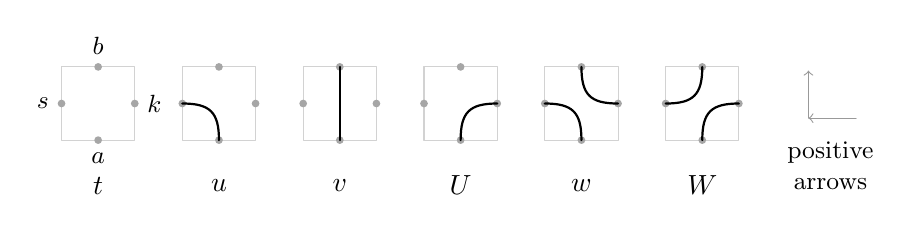
\begin{tikzpicture}[scale=.93,line cap=round,line join=round]
\foreach \j/\lab in {0/t,1/u,2/v,3/U,4/w,5/W} {
  \begin{scope}[shift={(1.65*\j,0)}]
  \draw[gray!35] (-.5,-.5) rectangle (.5,.5);
  \foreach \x/\y in {0/-.5,.5/0,0/.5,-.5/0}
    \fill[gray!70] (\x,\y) circle (1.5pt);
  \node at (0,-1.12) {$\lab$};
  \ifnum\j=0
    \node[below,font=\small] at (0,-.54) {$a$};
    \node[right,font=\small] at (.54,0) {$k$};
    \node[left,font=\small] at (-.54,0) {$s$};
    \node[above,font=\small] at (0,.54) {$b$};
  \fi
  \ifnum\j=1 \draw[thick] (0,-.5) .. controls (0,-.12) and (-.12,0) .. (-.5,0);\fi
  \ifnum\j=2 \draw[thick] (0,-.5)--(0,.5);\fi
  \ifnum\j=3 \draw[thick] (0,-.5) .. controls (0,-.12) and (.12,0) .. (.5,0);\fi
  \ifnum\j=4
    \draw[thick] (0,-.5) .. controls (0,-.12) and (-.12,0) .. (-.5,0);
    \draw[thick] (.5,0) .. controls (.12,0) and (0,.12) .. (0,.5);
  \fi
  \ifnum\j=5
    \draw[thick] (0,-.5) .. controls (0,-.12) and (.12,0) .. (.5,0);
    \draw[thick] (-.5,0) .. controls (-.12,0) and (0,.12) .. (0,.5);
  \fi
  \end{scope}
}
\begin{scope}[shift={(10,0)}]
  \draw[->,gray!80] (-.3,-.2)--(-.3,.45);
  \draw[->,gray!80] (.35,-.2)--(-.3,-.2);
  \node[font=\small,align=center] at (0,-.85) {positive\\arrows};
\end{scope}
\end{tikzpicture}
\caption{The six local connection weights in the row convention
\(B_{s,b;a,k}\). The first cell labels the bottom/right input ports
\(a,k\) and left/top output ports \(s,b\); positive arrows point upward
and leftward. A dot is a port; an unused port is vacant. For each
single-strand cell, its complementary pair of
ports has the same unoriented weight. Each strand may be oriented either
way, with the phase specified in the text. The two double-strand cells
are noncrossing.}
\label{a:local-cells}
\end{figure}


Local adjacent \(B\) acting on spatial slots also preserves the link image by the same diagram calculus drawn now with two bottom, two top vertical stubs and all other stubs propagating. Here \(u\) propagates a single occupied straight, \(v\) slides it past a vacancy, \(w\) propagates both, while \(U,W\) are cup/cap choices with factors \(c,c^t\) by the signed half-turns. Similarly \(C,A\) in insertion order across no seam and their transposes into the shorter spaces preserve link images (short cups/caps or vacant and single-spin propagation). In particular at \(\lambda=d_*,\eta=\pm i\), all loops have zero spinless weight and an exchange \(B\) preserves the all-empty coefficient on this image (also \(t=1\)).

\subsubsection{The honeycomb weights}

We have identified the loop weights in a finite row. We next identify the
positive physical specialization, where every occupied vertex has weight
$x_*$. At homogeneous \(z_i=1,\lambda=d_*,u=Q^{-1}\), diagram rows split each square into two trivalent vertices sharing an edge, carrying respectively the bottom-left and right-top ports. Each visited vertex contributes precisely \(x_*\) by the local weights, with at most one strand visiting it; these are honeycomb diagrams. More explicitly take \(h=(\sqrt3,0), v=(\sqrt3/2,3/2)\), vertices
\[
 P_{ij}=ih+jv,\qquad R_{ij}=P_{ij}+(h+v)/3
\]
(modulo horizontal period \(Nh\) on the cylinder); \(P_{ij}\) neighbors \(R_{ij},R_{i-1,j},R_{i,j-1}\). At \(u=Q^{-2}\) instead group bottom-right and top-left; the bases are \(h,v'=v-h\), and the pair displacement \(P'\to R'\) now \((v'-h)/3\), so the same honeycomb cylinder with a different grouping. The line between rows is a horizontal cut through perpendicular edges at their midpoints. Also at general nearby \(\lambda,u=Q_\lambda^{-1},z_i=1\), divide each cell by its empty weight to give the first honeycomb geometry with \(X_\lambda\) per visited vertex.

\subsubsection{A finite bound for boundary paths}

To pass from a finite-height cylinder to its stationary state, we require
an upper bound on the weight of each boundary arc. We derive it from the
honeycomb parafermionic identity of Duminil-Copin and Smirnov
\cite{DuminilCopinSmirnov2012}, with spin $5/8$. The same estimate also
controls crossings of a strip.

Take a bounded convex domain cut out along row-cut lines of the lattice and their rotated counterparts (by honeycomb symmetries); the boundary stubs are perpendicular edges ending at midpoints, never at corners. Fix a starting boundary midpoint \(o\). Sum over walks to edge midpoints \(p\), each walk visiting interior vertices self-avoidingly, changing edge at every vertex, depositing
\(x_*^{\#\mathrm{vertices}}\exp(-i\sigma\,{\rm wind})\), \(\sigma=5/8\), to \(F(p)\). Winding is the signed total turn in radians; include the trivial walk. At every vertex \(V\) inside, with neighboring midpoints as complex coordinates, we have
\[
 \sum_p(p-V)F(p)=0.
\]
Indeed an arrival without prior \(V\) from the edge side opposite \(V\) (including the trivial arrival if appropriate) groups with its two extensions through \(V\), by \(1+2x_*\cos((2+\sigma)\pi/3)=0\). The remaining arrivals from outside \(V\) to \(p\) have passed via \(q\to V\to r\) for the other two midpoints; pair with using \(q\to V\to p\) and the reversed excursion now ending at \(r\). The loop via \(r\) returning \(p\) closed back at \(V\) is simple with \(q\) outside (prefix from the boundary). For instance arrange \(q,r,p\) round \(V\) at angles \(0,2\pi/3,-2\pi/3\): that loop is positive and winding after the prefix adds \(5\pi/3-\pi/3=4\pi/3\), versus its negative for the partner. Their contributions cancel since \(\cos((2+4\sigma)\pi/3)=0\); reflection is identical.

Summing leaves only the boundary. Each path to another boundary midpoint has \(|{\rm wind}|\le\pi\) by closing from exit to entrance along the positively directed convex boundary (corner turns \(+\pi/2\) at each endpoint and intermediate boundary turn in \([0,2\pi]\)). Relative to the initial inward step the real parts thus contribute at least \(\cos((1-\sigma)\pi)\) times masses after dividing by half-edge length, while the \(o\) term contributes \(-1\). Exhausting a half-plane or strip by such convex polygons now bounds, by an absolute constant, the total \(x_*\)-mass of boundary arches from a given boundary midpoint in that half-plane, or bridges from a boundary midpoint reaching the parallel other boundary in the strip.


The honeycomb connective-constant theorem
\cite[Theorem~1]{DuminilCopinSmirnov2012} gives, for the number $c_m$ of
$m$-edge walks from a fixed vertex,
\[
 \mu=\lim_{m\to\infty}c_m^{1/m}=\sqrt{2+\sqrt2},\qquad x_*=\mu^{-1}.
\]
Consequently $x_*$ is the convergence radius for these edge-counted walks.
The boundary estimate also yields a quantitative upper bound by the
successive-extrema unfolding principle~\cite{HammersleyWelsh1962}; we give
the argument, including its lattice endpoint conventions.

For completeness, the boundary estimate itself implies that $x_*$ cannot
exceed the plane convergence radius. The endpoint conversion is also
needed in the quantitative estimate, so we give its details. Put \(Y=2\,({\rm vertical\ height})\); increments are nonzero integers of magnitude at most 2. For walks from a given vertex at one \(Y\)-extremum to their other extremum of specified \(Y\), confined between them (strictness not needed, span nonzero), the total \(x_*^{\#\mathrm{edges}}\) is uniformly bounded: extend to perpendicular cut midpoints just below and above the two extreme rows. At the minimum attach first a neighboring lower \(P\) if at an \(R\), and at the maximum a neighboring higher \(R\) if at a \(P\), by fixed conventions. Added vertices lie strictly outside the old heights, and the bridge bound applies with only bounded length adjustment. An arbitrary \(m\)-step walk splits at a lowest vertex. Along each arm going away, cut at the last highest vertex, then last lowest of the remainder, alternately until the end. The positive spans are decreasing strictly after a possible initial equality, and sum to at most \(2m\). Thus the original chronology is a concatenation of \(O(\sqrt{m})\) extremum-to-extremum bridges, some reversed back, with at most \((C m)^{O(\sqrt{m})}\) possible signed span lists. Multiplying the uniform bounds gives subexponential total \(m\)-step mass at \(x_*\). The matching opposite radius bound will also follow from the winding masses below.

In the notation just introduced, the quantitative conclusion is
\begin{equation}
 c_mx_*^m\le \exp\!\bigl(C\sqrt m\log(m+1)\bigr)
 \qquad(m\ge1),                                      \label{c4:unfolding}
\end{equation}
for an absolute constant $C$.  For each extremum-to-extremum bridge in
this decomposition, the extension adds $a,b\in\{0,1\}$ vertices at its
lower and upper ends.  An $l$-edge bridge therefore has port weight
$x_*^{l+1+a+b}$; the exterior half-edges add no visited vertices, and
inverse multiplicity is bounded.  These conversions preserve the uniform
piece bound used in the unfolding count.

\subsubsection{Existence and uniqueness of the normalized stationary state}

Return to a cylinder of fixed circumference $N$. The boundary-path bound
now proves convergence of the row iteration, rather than merely bounding
its matrix entries. At either homogeneous physical transfer,
\(\eta=\pm i\), consider the formal matching matrix at \(d_*\). It is nonnegative, loops killed. Its powers on the empty state increase coefficientwise since all-empty propagation is available. They are bounded: each remaining arc lifts to a planar arch in the lower half-plane from a given slot; a product of the just-proved bounds dominates each coefficient. Every nonempty matching \(J\) is reachable with positive coefficient: build one periodic arc at a time in decreasing interval length, extending already present ends vertically. No already occupied slot lies in the new intervals by noninterlacing. In one row a top-to-top arc can run horizontally between its two slots with positive allowed turns, simultaneously with the required vertical passes outside. Writing $T$ for the matching transfer, for each $J\ne\varnothing$
there are $m\ge1$ and $\epsilon>0$ such that
$T^m e_\varnothing\ge e_\varnothing+\epsilon e_J$ coefficientwise.
Consequently
\[
 0\le \epsilon T^n e_J
 \le T^{n+m}e_\varnothing-T^n e_\varnothing\longrightarrow0.
\]
Thus every nonempty basis vector is sent to zero in the limit. This gives a rank-one projection limit on the formal space (eigenvalue \(1\) simple, all others of modulus less than 1). Hence also on its spin image, with unique fixed vector normalized to empty coefficient 1 and obtained from vacuum by the transfer limit. At fixed \(\lambda=d_*,\eta=\pm i\), varying sites near homogeneous and fixing the auxiliary at a physical value, that simple normalized link eigenvector continues regularly with eigenvalue 1 (the empty coefficient of transfer is unchanged on this image). In particular uniqueness there also implies generic uniqueness if supplied with a rational normalized eigenvector.

\subsection{Polynomial formulas for the two stationary states}\label{c4:vacua}

The stationary states just obtained by a positive transfer limit have
rational continuations in the column parameters. We construct those
continuations explicitly. The two twists $i$ and $-i$ require different
polynomial degrees; both will be needed because adding their marked
observables retains winding polygons and cancels contractible polygons.

Throughout this subsection \(\lambda=d_*\). We use \(p=2,\eta=i=q^2\)
and \(p=1,\eta=-i=q^{-2}\), respectively. Put \(P=2+\sqrt2,\ K_2=P q^3,\ K_1=1+q^3\). For each choice we construct a polynomial vector $V_N(z)$ in the link
image, with \(V_0=1\) and \(V_1=|0\rangle\). When both constructions occur
in one formula, their choice is specified by $p$ or by the twist $\eta$.
The defining requirements are as follows:

\par\noindent\textbullet\quad Homogeneous \(z\)-degree \(p N(N-1)\). Each component on spins \(s_l\), divided by \(\prod_l z_l^{|s_l|}\) (called stripping), is polynomial in the \(t_l=z_l^2\), of degree per \(t_l\) at most \(p(N-1)-|s_l|\).
\par\noindent\textbullet\quad Exchange of adjacent arguments \(z_i,z_j\) (in order before exchange) acts by \(B_{ij}(z_i/z_j)\); rotation left acts by \(\Omega\).
\par\noindent\textbullet\quad For spin 0 at \(l\), the value at zero and the leading scale at infinity in \(t_l\) are respectively \(\prod_{k\ne l}t_k^p\) and \(t_l^{p(N-1)}\) times \(V_{N-1}\) with \(l\) removed.

Polynomial exchange equations and special-parameter reductions have
counterparts in other loop models. Garbali and Nienhuis study polynomial
exchange equations and fusion recurrences for dilute $O(1)$ ground states,
with determinant formulas for the associated sum
rules~\cite{GarbaliNienhuis2017Ground,GarbaliNienhuis2017Sum}. Here the loop
weight is zero, and both normalized vectors are constructed by the
interpolation argument below.

\subsubsection{Pair values and the two-site initial condition}

The degree and endpoint requirements do not by themselves determine
$V_N$. We prescribe its values when two column parameters have the cup
ratio. We impose pair prescriptions at \(z_j=Q^3 z_i\). For \(p=2\) prescribe one for every directed pair \(i\to j\) in the cyclic list. For \(p=1\) only require \(i<j\). First for an order \((\ldots,i,k_1,\ldots,k_r,j,\ldots)\), insert \(C\) at \(i,j\) made adjacent (just before the intermediate list) on \(V_{N-2}\) of the other sites, then transport \(j\) right to its specified position over the intermediate list by successive exchanges \(B(z_j/z_{k_l})\). Multiply by
\[
 \Pi_{ij}=K_p u^p\!\!\prod_{k\ne i,j}[(t_k-q^{-3}u)(t_k-q^6 u)]^p,\qquad u=t_i.
\]
Call the result \(W_{ij}\). For a cyclic prescription in construction \(p=2\), rotate to this situation (cut outside the directed interval) and rotate the result back by the inverse powers of \(\Omega\). The choice of linearizing cut does not matter using cyclicity of the smaller tensor: a block rotated over the cut when comparing two choices either misses this operation or contains the entire affected block, which conserves the total spin of its spectators; also \(\Omega^N=I\) on charge zero. These prescriptions respect site parity under stripping (including simultaneous signs at paired endpoints); this follows by the sign rule for exchanges and equal starting occupancies at the two ends of \(C\).

At \(N=2\) write \(V_2=D|00\rangle+H c\). Use
\[
 \begin{array}{c|cc}
 &D&H\\\hline
 p=2&t_1^2+(2+2\sqrt2)t_1t_2+t_2^2&P Q^3 z_1 z_2(t_1-t_2)/(1-q^3)\\
 p=1&t_1+t_2&(Q^3+Q^{-3})z_1 z_2 .
 \end{array}
\]
Indeed \(c^tc=0\); exchange sends \(H\) to \(U D+wH\), equal to \(-H,H\) respectively. By the weights at \(z_1/z_2=e^{ix}\), the ratios needed are
\(-U/(1+w)=-s_2\sin x/(\cos d_*+\cos(3d_*)\cos(2x))\) and \(U/(1-w)=s_2/(2s_3\cos x)\), giving the table. Rotation of \(c\) contributes scalar \(-1,1\) respectively. The prescribed adjacent pair values and other constraints now follow directly.

\begin{proposition}[The two polynomial vacua]\label{prop:polynomial-vacua}
For each of the choices \((p,\eta)=(1,-i),(2,i)\), there is a unique
polynomial family \(V_N\), \(N\ge0\), satisfying the degree, exchange,
rotation, deletion, and pair requirements above. It lies in the link
image, its empty coefficient \(D_p=V_N^{\rm empty}\) is not identically
zero, and
\[
                     T_\eta(z;u)V_N(z)=V_N(z)
\]
as a rational identity for every auxiliary parameter \(u\).
The normalized rational vector \(V_N/D_p\) extends regularly to
homogeneous sites and there equals the empty-normalized stationary state
obtained from either physical transfer limit.
\end{proposition}

\subsubsection{Compatibility of the pair prescriptions}

We prove Proposition~\ref{prop:polynomial-vacua} by induction in \(N\),
starting with the displayed initial vectors. The first step is to check
that the prescribed values agree wherever two pair slices meet.
All parameters not constrained by those slices are first taken
generic. Meromorphic continuation will then cover every regular
specialization. Each \(W_{ij}\) is covariant by ordinary adjacent swaps not swapping its two endpoints together. For endpoint \(j\) this follows by its transport definition and unitarity; for \(i\) moving past a slot \(k\) use
\(B_{12}(z_k/z_i)(I\otimes C)=B_{23}(z_j/z_k)(C\otimes I)\), or reverse by unitarity. For spectator swaps use smaller-tensor exchanges and the braid relation if both spectators lie on the transport route. For a cyclic interval one can linearize across a cut outside the route not splitting the swap (moving a cut past a whole swapping block is compatible by charge); the prescriptions are also covariant by rotation for \(p=2\).

It follows that evaluations from two disjoint prescribed pairs at their intersection agree: place both pairs positive-adjacent without swapping the endpoints of either together, and apply smaller-tensor prescriptions and commuting insertions. In the cyclic case one may migrate an end around over other labels up to adjacency (the second pair can cross the whole first block this way) and rotate both away from the seam. The products of prefactors agree: for start parameters \(u,v\) the extra cross factor before power \(p\) is \(q^6\prod_{k=\pm2,\pm3}(v-q^k u)\), symmetric. All swaps of unrelated labels here are generically invertible.

At two pairs with common start (so equal ends), arrange the triple consecutively preserving the orientations; transporting one equal end past the other uses \(B(1)=I\). For common end, similarly use \(B_{23}(Q^3)(C\otimes I)=I\otimes C\); again values agree. At a chain intersection \(i\to j\to k\) both evaluations vanish: \(\Pi\) has an order-\(p\) zero at the third parameter, with at most one exchange pole there; when \(p=1\), \(i<j<k\) and the third parameter in either prescription is outside its transport route, so not a pole at all.

\subsubsection{Interpolation and polynomial degree bounds}

Assume that the smaller tensors have been constructed. We now construct
$V_N$, check that the apparent interpolation poles cancel, and prove its
bounds in every parameter. For \(N\ge3\), interpolate after stripping in
\(t_N\). Use nonzero nodes
\[
 r_{i\epsilon}=q^{3\epsilon}t_i,\qquad i<N,\quad
 \epsilon\in J_p,\qquad J_1=\{1\},\ J_2=\{1,-1\}
\]
by those prescriptions (\(z_N=Q^{3\epsilon}z_i\)), and also zero with the required deletion input if \(s_N=0\). With \(\rho=[s_N=0]\), the Lagrange factors for nonzero nodes are
\[
 L_{i\epsilon}=(t_N/r_{i\epsilon})^\rho
       \prod_{(a,\gamma)\ne(i,\epsilon)}\frac{t_N-r_{a\gamma}}{r_{i\epsilon}-r_{a\gamma}} .
\]
Use \(L_0=\prod_{a,\gamma}(1-t_N/r_{a\gamma})\) when needed. Homogeneity and charge zero hold, and the result unstripped stays in the link image since the extra scaling and interpolation weights depend only on occupancy at \(N\). Each prescribed input \(W\) is polynomial on the paired slice after stripping: every transport pole divisor involving the paired parameter and a spectator is canceled by \(\Pi\); at spectator zero the matrices stay bounded and parity suffices to strip, at simultaneous endpoint zero even the \(u^p\) supplies divisibility. Its stripped spectator degree has the desired bound since \(\Pi\) adds \(2p\) there, the raw smaller tensor grows by at most degree \(p(N-3)\), and bounded exchange and stripping then give the bound by parity (rounding down to integral degree).

Potential interpolation poles at coincident nonzero nodes from \(t_i=t_l\) cancel between the corresponding simple Lagrange poles by common start/end compatibility, and at \(t_i=q^{\pm6}t_l\) for \(p=2\) by chain vanishing. At \(t_l\to0,\infty\) for \(l<N\), the special terms \(i=l\), including stripping and Lagrange factor, grow respectively at worst as
\[
 O(t_l^{\,1-(|s_l|+|s_N|)/2-\rho}),\qquad
 O(t_l^{\,p(N-1)-(|s_l|+|s_N|)/2-\rho});
\]
indeed the raw paired input has bounds from \(\Pi\) of powers \(p,\ p(2N-3)\), and the other factors of \(L_{l\epsilon}\) beyond \((t_N/r)^\rho\) contribute at worst powers \(-(p-1),-p(N-2)\). These bounds have no pole and give the required degree (round by parity), subleading at infinity for vacant \(l\). In other terms use the spectator bounds and the zero input factor \(t_l^p\) canceling the \(L_0\) pole. Thus all coefficients are polynomial after stripping with the claimed degrees.

\subsubsection{Deleting a vacant spectator}

We have a polynomial vector with the required degrees. To complete the
induction, its deletion limits must agree with the smaller tensors in
every variable, not just in the interpolation variable. Fix a spectator
\(l<N\) with \(s_l=0\). At infinity, in nonspecial pairs only the smaller-tensor vacant \(l\) can contribute to the leading scale; if crossed it is passed exactly by the extreme swap. Thus these give \(t_l^{p(N-1)}\) times smaller interpolation terms (power \(2p\) from \(\Pi\) and \(p(N-3)\) from the smaller-tensor deletion, removed Lagrange factors tending to 1); the zero term likewise, special terms subleading as above.

At zero the nonspecial inputs scale to smaller inputs times \((\prod_{k\ne l,N}t_k^p)r_{i\epsilon}^p\), since the dropped spectator factors in \(\Pi\) give \(q^{3p}u^{2p}\); their extra Lagrange factors tend to \((t_N/r_{i\epsilon})^p\). These yield the nonzero-node terms needed after deletion. Special terms vanish if \(s_N\ne0\). Suppose \(s_N=0\) and write \(L'_0\) for the smaller zero basis. For \(p=2\) the special raw inputs before stripping at leading order are
\[
 P q^{3\epsilon} t_l^2 \!\!\prod_{k\ne l,N}t_k^4\, V_{N-2},
\]
as both endpoints remain vacant and the traveling end swaps exactly at leading order. Rotations if needed here and for spectator deletion do not pick up a phase from crossed vacancies. Multiplication by \(L_{l\epsilon}\sim t_N^2L'_0/[q^{3\epsilon}(q^{3\epsilon}-q^{-3\epsilon})t_l^2]\) gives cancellation. The ordinary zero input then yields the required zero term using the smaller-tensor deletion \((L_0\sim (t_N/t_l)^2L'_0)\). For \(p=1\) the special raw input is similarly at leading order
\((1+q^3)t_l\prod_{k\ne l,N}t_k^2 V_{N-2}\), with \(L_{l+}\sim t_N L'_0/(q^3 t_l)\), while the zero input has leading raw \(t_l\prod_{k\ne l,N}t_k^2 V_{N-2}\), with \(L_0\sim-t_N L'_0/(q^3t_l)\). These combine to exactly the desired zero term. Stripping spectator factors is common to all of these comparisons. This proves both deletion limits for \(l<N\); vacant \(t_N=0\) is already a node.

\subsubsection{All pair values, exchanges, and rotation}

The degree bounds and spectator deletions now let us test the remaining
identities by interpolation. First impose every required pair
\(i\to j\) not involving \(N\) by comparing as polynomials in spectator \(t_N\) on the slice. At the same nonzero interpolation nodes (still distinct generically), compatibility gives equality, and at zero if vacant use spectator deletion in \(W_{ij}\) by the same \(\Pi\), smaller-tensor and extreme-swap rules. Degree in \(t_N\) after stripping then proves the prescription.

For \(p=1\) deduce now the vacant infinity deletion at \(N\) as well: the difference in the leading coefficient from the required one, stripped, has all factors \(t_j-q^3t_i,\ i<j<N\), by the pair prescriptions and smaller-tensor infinity limit. Its total degree is at most \((N-1)(N-2)/2\), strictly less for any nonvacuum spin list. For the all-vacant component use also \(t_l=0\) for some \(l<N\) (the deletion limit there with smaller-tensor infinity gives agreement). Thus the difference vanishes.

Exchanges for either construction follow by testing a third label's parameter (\(N\ge3\)). At all pair nodes involving that label the pair covariances apply (its order relative to the partner is unchanged if \(p=1\)); at zero for a vacant spin use deletion. These suffice by degree since the exchanged sites are external to the variable being tested. Similarly for \(p=2\) test any label's parameter to show rotation using the cyclic covariances of the prescriptions and zero deletion. This also gives the remaining infinity deletion at \(N\) for \(p=2\).

Only rotation for \(p=1\) remains. Its pair prescriptions were imposed in
linear order, so cyclic covariance is not already available.
Consider the difference between \(V_N\) at the left-rotated list and
\(\Omega V_N\). All ordered pair specializations among labels
\(2,\ldots,N\) vanish by smaller-tensor cyclicity (the pair transport
misses slot 1); the vacant deletion limits for these labels vanish too
(difference at the specified leading scales). Thus any component vacant
at one of \(2,\ldots,N\) vanishes identically using \(N-2\) pair roots
there, zero and the infinity coefficient. The difference is supported on
that tail all occupied, and exchanges by \(B\) on the tail by what was
just proved. Projecting an exchanged adjacent pair to \(00\) forces
\(c^t\) annihilation there; hence the exchange acts by scalar
\(w(z_i/z_j)\) alone. Its poles now force both factors
\(t_j-q^2t_i,\ t_j-q^3t_i\) in the stripped polynomial for every
\(2\le i<j\le N\), by bringing these arguments adjacent (other generic
swaps nonsingular); the \(w\) numerator is nonzero generically there.
This exceeds the degree \(N-2\) per occupied variable since \(N\ge3\).
Hence rotation holds. We have finished the induction for both
constructions. Uniqueness follows from the same interpolation nodes and
degree bounds at each induction step.

\subsubsection{The empty component and the transfer fixed vector}

It remains to normalize the constructed vector and identify it with the
physical stationary state. Write \(D_p=V_N^{\rm empty}\), the coefficient
of the all-vacant spin tensor. It is symmetric by exchanges and link loop killing. In fact with \(X=(t_i)\)
\[\begin{gathered}
 D_2(X)=P^N\!\prod_{i<j}\left[\frac{p_K(t_i,t_j)}{t_i-t_j}\right]^2 \det[k(t_i,t_j)],\\
 p_K(x,y)=x^2+\sqrt2xy+y^2,\quad k(x,y)=xy/p_K(x,y).
\end{gathered}\]
Indeed this expression is polynomial (all \(p_K\) poles canceled and a Vandermonde zero in each of rows and columns). It has both required endpoint limits by inspection (in particular correct maximum degree). At \(t_j=q^3u,\ u=t_i\), the double pole term \(-k(u,t_j)^2\det k_{\rm red}\) in the determinant gives exactly \(\Pi_{ij}\) times the smaller formula: \(-P^2 q^6/(1-q^3)^2=P q^3\) and the extra spectator factors reduce by factoring \(p_K\). These and the vacant zero input suffice by interpolation since the constructions of \(W\) preserve the inserted empty coefficient apart from \(\Pi\). The inversion formula \(D_2(X^{-1})=\prod_i t_i^{-2(N-1)} D_2(X)\) follows. We do not need an analogous determinant here for \(D_1\). Both denominators are generically nonzero, also on slices of a pair at ratios \(q^{\pm1,\pm2,\pm3}\) (meaning either sign in any of the three powers), by deletion down to the displayed two-site components.

We next prove the fixed-vector identity
$T_\eta(z;u)V_N(z)=V_N(z)$ for every auxiliary parameter $u$, as a rational
identity. This is the step connecting the interpolation construction to
the transfer limit. Induct using one site variable \(t_l\); clear its two transfer pole factors and strip its output-spin parity. The difference has degree at most \(p(N-1)+2-|b_l|\) at output spin \(b_l\), by bounded extremes and rounding as before. It vanishes at the \(p(N-1)\) prescribed pair nodes involving \(l\), by \(W\), placing the pair adjacent and using \(C\)-transparency and smaller transfer (intertwining the swaps/rotations). At zero if \(b_l=0\) use deletion and extreme swap. It also vanishes at \(t_l=u^2\) and \(t_l=q^3u^2\) for auxiliary \(u\). Indeed put the site last in the first case \(z_l=u\): \(B(1)\) identifies \(s_{N-1}=a_N,\ s_0=s_N=b_N\) in row notation. The exchanges in the remaining row move the last argument left through all to the first position; the twist factor \(\eta^{b_N}\) undoes this rotation.

In the second case put the site first with \(z_1=Q^3u\); \(CC^t\) forces \(s_0=-b_1,\ s_1=-a_1\) with factor \(q^{a_1-b_1}\). Cross the remaining
\(B(z_i/u)_{s_{i-1},b_i;a_i,s_i}=q^{a_i-b_i}B(z_1/z_i)_{b_i,-s_i;-s_{i-1},a_i}\).
Phases cancel by charge, and this braid moves the first argument right to last while the twist again undoes rotation. The node count is sufficient (start the induction at \(N=0\)).

Set \(\Psi_\eta=V_N/D_p\); we call this normalized stationary vector the
\emph{vacuum}. These normalized rational vectors are regular by continuation at homogeneous sites and give exactly the physical transfer limits: even if a denominator representation vanishes there, generic uniqueness near those sites identifies the rational function locally with the regular link eigenvector already established. All exchanges/rotation, endpoint deletions with vacuum normalization (nonvacant outputs vanishing by the degree bounds), spin parities and transfer fixed identities thus hold in the stated limits or as rational identities.
This completes the proof of Proposition~\ref{prop:polynomial-vacua}.

\subsection{A marked row and its polygon interpretation}\label{c4:marked-row}

A closed transfer kills every loop when $\eta=\pm i$. To retain one loop,
we fix the orientation of a single auxiliary edge instead of summing it.
The resulting scalar has opposite signs on contractible polygons for the
two twists. We will first establish its finite algebraic properties and
then compute those signs geometrically.

Set \(\lambda=d_*\) and \(\eta=\pm i\). For an operator $H$ on the
$N$-site spin space, use the normalized rational vectors just constructed
to define the bilinear bracket
\[
 \langle H\rangle=\Psi_\eta(z^{-1})^t H\Psi_\eta(z),\qquad
 Z_\eta(y)=\langle M_{-,-}(z;\sqrt y)\rangle.
\]
Here $z^{-1}=(z_1^{-1},\ldots,z_N^{-1})$, and the symbols $-$ in
$M_{-,-}$ mean the auxiliary spin $-1$ at both ends of the open row.
Write \(P_{l,s}\) for the projector to spin \(s\) at site $l$.

\subsubsection{Normalization and pair reductions}
 One has \(\langle I\rangle=1,\ \langle P_{l,+}+P_{l,-}\rangle=0\): gluing two link states, read the bra as arcs \emph{above} with inverse twist (the arc turning and factors in its coefficients then have exactly the indicated signs). For a loop with signed left seam crossings \(N_L,N_U\) below and above respectively, the twist factor is \(\eta^{N_L-N_U}\), real (\(\pm1\)) if contractible and imaginary (\(\pm i\)) if essential, since \(N_L+N_U=0,\pm1\) respectively. The free orientations thus sum to zero by the turning phases. Occupancy restriction does not interfere, and the all-vacant coefficients are normalized.

By exchanges, transpose symmetry, unitarity and row intertwining, \(Z_\eta\) is symmetric in the site labels, rational in the \(t_i\) and \(y\) by the sign rule and site parity. In \(y\) poles can only come from \(\prod_i(y-q^2t_i)(y-q^3t_i)\), and both endpoints \(0,\infty\) give 1 since the weighted extreme swaps have total spatial charge zero, the scalar on each is 1 and one-way flips cannot restore the fixed auxiliary. Also sending a spectator \(t_k\) alone to either endpoint decouples that site, by the vacant leading limits of the vectors in both factors of the brackets and the extreme swap past a vacancy. At \(a=t_l\) one has the crossing value
\[
                         Z_\eta(a)=Z_\eta(q^{-3}a).
\]
Indeed put \(l\) last at \(y=a\); \(B(1)=I\) forces its output spin equal to the traced seam spin. Thus \(M_{-,-}\Psi_\eta=\eta P_{\rm last,-}\Psi_\eta\) by projecting \(T_\eta\Psi_\eta=\Psi_\eta\). At \(y=q^{-3}a\) put \(l\) first and \(B(Q^3)=CC^t\) similarly gives \(\eta P_{\rm first,+}\Psi_\eta\). Rotating both ket and bra from first to last multiplies the charged projector contractions by \(\eta^{2(\pm1)}=-1\); use the projector-sum vanishing.

Pair reductions hold rationally for otherwise generic variables, including generic \(y\): two site parameters \(t,q^2t\) replace by the single \(qt\), and \(t,q^3t\) delete. Arrange them ordered adjacent (across no seam) and use positive root ratios \(z_j/z_i=Q^2,Q^3\) respectively. The vacuum denominators in either order and either set of inverse arguments are nonzero generically on these slices by the decoupling limits down to the size-two vacua. In positive order the exchange \(B(Q^2)=A A^t\) or \(B(Q^3)=C C^t\) from reverse order places \(\Psi_\eta\) in the inserted image. Extract \(A\) or \(C\) by its left inverse. The result stays in the link image (\(A^t A\) diagonal \(1,2x_*^2,2x_*^2\), inverse just occupancy scaling, \(C^t C=1\)), has empty coefficient 1, and is a transfer fixed vector on the fused/deleted list by the spatial \(A,C\) transports, hence the corresponding shorter vacuum by generic uniqueness there.

In inverse-site arguments the order is opposite: exchange to positive order uses \(A A^t\) or \(C C^t\) on \(\Psi_\eta(z^{-1})\). By the result for positive order and injectivity, applying the transposed insertion alone thus yields exactly the shorter inverse vacuum. The same spatial transport identities hold in the open row, proving the pair reductions after contraction.

\subsubsection{The sign of a marked polygon}

We can now interpret the marked scalar at physical weights. The algebraic
states are complex, but the $-i$ marked observable will be a sum of
positive polygon weights. At homogeneous sites interpret
\(Z_\eta(q^{-k})\), \(k=1,2\), by surrounding the open row with the same physical rows (\(u=Q^{-k}\)) but twist \(\eta\) below and inverse twist above, vacuum on the two outer cuts, taking height limits. This gives the brackets by the transfer convergence and the crossed transpose identity. Draw first in oriented square topology as before, seam vertical. The right arrow fixed by the mark at its seam edge singles out a loop. All others sum to zero as before. Twist crossings of the marked loop now exclude the single marked crossing, and still use \(\eta^{N_L-N_U}\).

If contractible positive (counterclockwise), just before that right arrow on the seam upwards one is outside the loop, and just after one is inside; \(N_L=0,N_U=1\). For the negative loop \(N_L=1,N_U=0\). The two possible full phases are \(q^{-2}\eta^{-1}\) and \(q^2\eta\), both \(-1\) at \(\eta=i\), \(+1\) at \(-i\).

For net rightward essential, the point just before is in the bottom component and \(N_L=N_U=0\); for net left it is in the upper component and \(N_L=N_U=1\). Indeed crossings toggle sides, right arrows entering the left side of the oriented strand, and the net sign over the full seam records which component is which. Both essential phases are 1.

Similarly \(Z_\eta(1)=\eta\langle P_{\rm last,-}\rangle\) can use \(u=Q^{-1}\) on both sides, marking a downward arrow and a seam just to its right (the point on the cut there is thus on the left side of the arrow). For counterclockwise contractible \(N_L=-1,N_U=1\); for clockwise both 0, giving the same signs with the extra \(\eta\). For net right essential \(N_L=-1,N_U=0\); for net left \(N_L=0,N_U=1\), again total phase 1 including \(\eta\).

Consequently each marked value at minus twist counts both essential and contractible self-avoiding polygons through its edge with weight \(x_*^{|\gamma|}\) (\(|\gamma|\) the length), and at plus twist essential minus contractible. These statements pass to the limit since the minus sign choice of \emph{twist} made both sums positive and their limiting bracket finite. The orientation of the marked loop is uniquely fixed. The three edges for \(1,q^{-1},q^{-2}\) sample exactly one of each honeycomb edge type up to lattice translations, on the same cylinder: the first two are across vertical and horizontal diagram ports of the first grouping (\(h,v\)); the third is across a horizontal port of the second (\(h,v-h\)), hence an internal pair edge of the first.

\subsection{Finite identities for marked polygon masses}\label{c4:color-sum}

The marked-row interpretation reduces the winding mass to two finite
scalar calculations. The first computes the sum of all polygon masses
through one edge of each type. The second expresses the winding part as
a ratio of finite color sums. All identities are proved with generic
column parameters and then continued to the homogeneous cylinder.

Write \(d=q+q^{-1}=\sqrt2,\ P=2+d,\ c_*=2-d=2/P\). Use site list \(X=(t_i)\) and \(a\in X\) a distinguished parameter. Set
\[
 S'_{\eta,a}= Z_\eta(a)+ Z_\eta(q^{-1}a)+ Z_\eta(q^{-2}a),\qquad S_a=c_*+S'_{i,a}
\]
(where \(i\) in the twist denotes \(\sqrt{-1}\)). All unspecialized parameters in residue arguments are otherwise generic.

For a spectator \(b\), possible row poles of \(S'\) beyond vacuum denominators are \(b/a=q^{3,4,5,6}\). At \(q^3,q^5\) those collisions do not give poles: on the slice, the colliding \(y\)-residue of \(Z(y)\) vanishes by pair deletion, with that pole branch simple and disjoint from other \(y\)-poles and vacua regular generically. This gives boundedness when approaching in \(b\) with \(y\) fixed. At \(b=q^2 a\) there is no collision, and \(S'\) takes the shorter value at the fused mark \(q a\) by pair reduction and crossing there. At \(b=q^{-2}a\) the same holds with fused mark \(q^{-1}a\) by replacing \(Z(a)\) by \(Z(q^{-3}a)\) via crossing \emph{before} specializing. Also \(S'_a=S'_b\) (at fixed twist) for \(b=q^{\pm1}a\) by crossing.

\subsubsection{The sum of all polygon masses}

We first prove the rational identity
\begin{equation}\label{a:minus-scalar}
                              S'_{-i,a}=c_*.
\end{equation}
This is true for \(N=1\), whose three terms are \(0,x_*^2,x_*^2\). Write \(D_-=D_1\) and \(D_+=D_2\) for the two vacuum polynomials (minus and plus twist). Multiply the inductive error by \((b+a)D_-(X)b^{N-1}D_-(X^{-1})\). This clears all non-monomial poles in \(b\) (at \(-a\) row poles before vacuum division are at most simple). Both endpoints of the error vanish by spectator decoupling and induction. Thus the product is polynomial of degree \(\le2N-2\) and has a zero at 0. Other zeros are at \(b=q^{\pm2}a\) and \(b=q^j a'\) for every other spectator \(a'\ne b\), \(j=\pm2,\pm3\), by pair reductions. For $N\ge2$ these are
$1+2+4(N-2)=4N-5$ distinct zeros at generic parameters, more than the
degree bound $2N-2$. The polynomial therefore vanishes.

\subsubsection{An unmarked determinant and a finite color sum}

For the winding mass we need a second scalar representation. Set
\[
 \begin{gathered}
 p_K(x,y)=x^2+dxy+y^2,\qquad \delta(x,y)=p_K(x,y)(x^2+y^2),\\
 R_X=\frac{D_+(X)^2}{\prod_{x,y\ {\rm pair\ in}\ X}\delta(x,y)}
   =P^{2|X|}(\det k_X)^2\prod_{x,y\ {\rm pair\ in}\ X}
           f(x,y),\\ f(x,y)=\frac{p_K(x,y)^3}{(x-y)^4(x^2+y^2)} ,
 \end{gathered}
\]
using unordered pairs and \(k=xy/p_K\). Define colors \(-,0,+\) with weights \(\ell_-=(-1-d+i)/2,\ \ell_0=P,\ \ell_+=q\ell_-\). Put \(G(r)=(1+r)^2/[(r-q)(r-q^{-1})]\), \(\beta=G(1)=2P\), so \(\sum\ell=1,\ \ell_-\ell_+=P^2/\beta\). For sites \(x,y\) of colors \(s,t\) multiply a pair factor \(g_{st}(y/x)\), with table
\[
 g(r)=\begin{pmatrix}
 1&G(r/q)&G(r/q)G(r/q^2)\\
 G(rq)&G(r)&G(r/q)\\
 G(rq)G(rq^2)&G(rq)&1
 \end{pmatrix}.
\]
For a color assignment $\sigma:\{1,\ldots,N\}\to\{-,0,+\}$
define its weight to be
\[
 \prod_{j=1}^N\ell_{\sigma(j)}
 \prod_{1\le j<k\le N}g_{\sigma(j),\sigma(k)}(t_k/t_j).
\]
The relation $g_{st}(r)=g_{ts}(1/r)$ makes the sum invariant under
reordering the sites. Let $\tau_X$ be the sum of these weights over all
$3^N$ assignments. Let $F_X(y)$ be the same sum with the additional factor
$\prod_{j=1}^N L_{\sigma(j)}(t_j/y)$. To define these factors, put
\(f_j(r)=1-q^j r\) and
\[
 L_-=L=\frac{f_5 f_6 f_7}{f_2 f_3 f_4},\qquad
 L_0(r)=\frac{L(r/q)}{L(r/q^2)},\qquad L_+(r)=1/L(r/q^3).
\]
The sums do not depend on site order.

\subsubsection{Residues and the determinant identity}

We prove $R_X=\tau_X$ by showing that both rational functions have the
same residues and the same limits when one parameter tends to zero or
infinity. The decorated sum has the same reduction rules, which we will
need for the marked identity.

Here are the residues in either color sum between sites \(a',b\), using coordinate \(b/(q^j a')-1\). At \(b=q^2a'\) (\(j=2\)) one gets factor \(\alpha P\), \(\alpha=P/(q-q^{-1})\), times \(\prod_{z\ne b,a'} G(z/(q a'))\) times the same sum on the list fused to \(q a'\). Indeed pairs \((-,0),(0,+),(-,+)\) contribute, fusing to \(-,+,0\) respectively, by the simple \(G\)-residue \(\alpha\) and the color weights above. Their spectator table products with a spin \(s\) reduce by
\(g_{i,s}(r)g_{j,s}(r/q^2)=G(r/q)g_{k,s}(r/q)\)
for each fusion \(ij\to k\), \(r=z/a'\); \(L_i(t)L_j(q^2t)=L_k(qt)\). At \(b=q^3 a'\) only \((-,+)\) contributes, with factor \(\alpha G(q^2)P^2/\beta\), spectator factors \(G(r/q)G(r/q^2)\), and the pair deleted (decoration cancels). At \(b=q a'\), \((0,0)\) and \((-,+)\) residues cancel by the table and common decoration \(L(t)/L(q^{-2}t)\). Equal-site simple poles cancel by symmetry, and inverse ratios are treated by exchange. These checks for \(F_X\) hold at generic \(y\) and regularly for decorations away from their poles.

Then \(R_X=\tau_X\). Indeed \(R_X\) has only the simple pole loci above with \(j=\pm2,\pm3\). At \(b=q^3a'\), the empty-component pair prefactor in \(D_+\), squared over the \(\delta\) cross factors, yields exactly \(G(r/q)G(r/q^2)\) per spectator (remaining numerator roots \(q^5,q^6\) double, denominator roots \(1,q,q^2,q^3\)). At \(b=q^2a'\) use kernel Schur complements. For an ordered list $Y$ for which the
matrix $k(Y,Y)$ is invertible, define
\[
 k_Y^\perp(s,t)=k(s,t)-k(s,Y)k(Y,Y)^{-1}k(Y,t).
\]
The required identity, with \(Y=(a',q^2a')\) and \(Y'=(qa')\), is
\[
 k_Y^\perp(s,t)=H(s/a')H(t/a') k_{Y'}^\perp(s,t),\qquad H(s)=(s^4-1)/(s^4+1).
\]
To see this scale \(a'=1\). The kernel \((1-H(s)H(t))k=2st(s^2-dst+t^2)/[(s^4+1)(t^4+1)]\) has rank three and agrees with \(k\) on the conditioning rows/columns at \(Y\) (the index matrix has diagonal \(1/P\), off diagonal \(1/d\)). Subtracting the \(Y\)-projector \(k(\cdot,Y)k(Y,Y)^{-1}k(Y,\cdot)\) leaves rank one in the same polynomial span vanishing at \(1,i\), hence proportional to \(H(s)k(s,q)H(t)k(t,q)\). At \(s=q\) comparing the \(H\)-pole gives multiplier \(-P\), as required.

Thus the squared determinant gains $H(r)^4$ per spectator relative to
fusion. Factoring the remaining pair terms gives
\[
 H(r)^4\frac{f(r,1)f(r,q^2)}{f(r,q)}=G(r/q).
\]
Only the two residue constants remain. At $N=2$ one has
\[
 R_{(1,b)}=\frac{(v+2+2d)^2}{(v+d)v},\qquad v=b+b^{-1},
\]
whose residues are exactly $\alpha P$ and
$\alpha G(q^2)P^2/\beta$. The cases $N=0,1$ start the induction.
For larger $N$, the reduction formulas now show that all residues of
$R_X$ and $\tau_X$ agree. Both functions have the same decoupling limits
at zero and infinity, so their difference is zero.

\subsubsection{Decorating the distinguished site}

The three edges in the marked observable correspond to three equal
specializations of the decorated color sum. More precisely, the quantities
\(F_X(a),F_X(q^{-1}a),F_X(q^{-2}a)\) coincide; denote their common value by
$F_a(X)$. They all equal one half the color sum on spectators with extra factors \(H_s^v(z/a)\) given in order by
\[
                 L,\quad 1,\quad f_1 f_2 f_3/(f_4 f_5 f_6)=q^{-1}L(1/r).
\]
Here the last expression uses argument \(r\) (as do the \(f_j\)'s). Indeed the surviving color \(k\) at \(a\) for these arguments \(y\) is \(-,0,+\) respectively, with \(\ell_k L_k(a/y)=1/2\), and \(g_{k,s}(r)L_s(ra/y)=H_s^v(r)\) by substitution (use \(G=f_4^2/(f_1f_7)\)). Denote the spectator sum without half by \(\tau^v\).

\subsubsection{The marked scalar identity}

We now prove the final finite algebraic identity:
\begin{equation}\label{a:marked-scalar}
                               S_a R_X=4c_* F_a .
\end{equation}
The pair reductions determine all residues except three simple pole
locations relative to the marked parameter. Symmetry then reduces the
possible error to a small polynomial ambiguity, which is removed by the
explicit one-, two-, and three-site calculations below.
Write \(J_a\) for left minus right. Inductively this vanishes as any spectator \(b\to0,\infty\) by decoupling (at infinity \(\ell_- q+P+\ell_+q^{-1}=1\)).

Vacuum denominators beyond those of \(R_X\) cancel by the \(D_+\) inversion formula. Residues at \(b=q^j a'\), \(j=\pm2,\pm3\), for another spectator match by pair reductions and the common \(F_X,R_X\) factors, all decorations regular at generic such points taking \(y=a\).

At \(b=q^{\pm2}a\) residues match similarly by reduction to the fused mark; take the specialization \(y=a,q^{-2}a\) respectively for \(F_X\), decorations regular there and at the fused site. At \(b=q^{\pm3}a\), \(S_a\) is bounded as noted above and \(F_a\) has at most simple poles by \(H^v\).

Thus the only poles left for \(J_a\) can be simple at \(b/a=q^{\pm3},-1\). Also at \(b=q^{\pm1}a\), \(J_a=J_b\) by the crossing consequence above and taking a common specialization for \(F_X\) (all decorations regular in a neighborhood, the pair pole removable by the cancellation already shown). Hence for \(m=N-1\) spectator ratios \(r_j=t_j/a\), \(t_j\in X\setminus\{a\}\), by symmetry and homogeneity,
\[
 J_a=\left(\prod_j B_0(r_j)\right)\sum_{j=0}^m c_j e_j(r),\qquad
 B_0(r)=\frac{r}{(r-q^3)(r+1)(r-q^{-3})},
\]
with \(e_j\) elementary symmetric: after factoring out the poles and endpoint zeros only degree \(\le1\) per ratio remains. The constants are label-independent. At \(b=q^\epsilon a\), \(\epsilon=\pm1\), a further ratio \(q^{3\epsilon}\) cannot be a pole, by the equality with \(J_b\), so
\[
                  c_j+\epsilon i d\,c_{j+1}-c_{j+2}=0\quad(0\le j\le m-2).
\]
Subtracting the two relations with $\epsilon=\pm1$ gives
$c_1=\cdots=c_{m-1}=0$. If $m\ge3$, either relation then also gives
$c_0=c_m=0$. For \(m=2\) remains \(c_0=c_2,c_1=0\); for \(m=1\) use \(B_0(1/r)=rB_0(r)\) in the same equality to give \(c_0=c_1\).

\paragraph{The three initial evaluations.}
The preceding reduction proves the induction once the remaining
ambiguities at \(N\le3\) have been removed. We compute them explicitly. For \(N=1\), \(S=2c_*,R=1,F=1/2\). For \(N=2\) take \(b=a\); the normalized plus vacua have vanishing occupied part, so \(S=c_*+2/P^2\), \(R=2P\), \(2F=1+P\) (each charged contribution \(1/2\)); equality holds.

For \(N=3\), the remaining error is
\(c_0B_0(r_1)B_0(r_2)(1+r_1r_2)\). Take site \emph{root} parameters
\(z=(1,\rho,\rho^2)\), \(\rho=e^{2\pi i/3}\), and \(a=1\). Their
squared spectator ratios are \(r_1=\rho^2,r_2=\rho\), so
\(r_1r_2=1\) and the factor multiplying \(c_0\) is finite and nonzero.
It therefore suffices to verify the identity at this triple. We first
compute \(R\) and \(F\), and then \(S\). Directly
\[
 R=P^6[(1/P+2/(d-1))(1/P-1/(d-1))^2]^2[-(d-1)^3/9]^3=1-d
\]
using the cubic ratios in \(k,f\). Also \(2F=1-d\): let \(r=\rho^2\), so spectator sites are \(r,1/r\) with ratio \(r\), and put \(A(r)=\ell_- L(r)\); the weights including \(H^v\) at \(r\) are \(A(r),P,A(1/r)\). For details, multiplying the displayed rational factors using \(r^2=-1-r,\ q=(1+i)/d\) gives
\[
 \begin{aligned}
 A(r)&=-(29+21d)/2-q^2(12d+17)(r+1/2),\\
 A(r)G(r/q)&=1/2+(q^3+q^2+q)(2r+1)/6,\\
 A(r)^2G(r/q)G(r/q^2)&=3/2+d+(4q^3+5q^2+4q)(2r+1)/6 .
 \end{aligned}
\]
The two like-charge contributions each give \(A(r)A(1/r)=-2-3d/2\); each unordered mixed-vacancy type gives \(P\), the opposite-charge type \(3+2d\), and the \(00\) term \(P^2G(r)=-2-2d\). This yields the stated value.

By rotation and common scaling, the two normalized plus vacua at this triple and its inverse (regular by the determinant) are vacuum plus pair terms with amplitudes \(h_{12}=h_{23}=-h_{13}=h\) and similarly \(h'\) respectively (in the link image each ordered nonwrapping pair has spin weights \(q^s\), the complementary wrap just gains scalar \(-1\)). Swapping sites 2 and 3 takes the triple to its inverse via \(B(\rho^2)\), so
\[
 h'=U+wh=(u-v)h,\qquad h h'=(u-v)U^2/(u-v-w)^2=-P.
\]
Indeed with \(a_j=\sin(j\pi/8-2\pi/3), s_2=\sin(\pi/4)\) the last quotient is
\[
 \frac{(s_2 a_0)^2(s_2-a_0)}{a_2a_3a_5(s_2-a_0-a_6)^2}
 =\frac{-48(d+\sqrt3)}{(\sqrt6+d)(d-1)(3d+2\sqrt3-\sqrt6)^2}.
\]
At twist \(i\), the regular marked projector formula gives \(Z(1)=i(2q^2 hh')=2P\) (put parameter 1 last cyclically, just rescaling the triple). By scaling and symmetry \(Z(y)\) here is invariant by \(y\mapsto \rho y\), has endpoints 1 and two simple pole orbits. Thus \(Z(y)=1+(2P-1)g(y^3)/g(1)\) with \(g(t)=t/[(t-q^6)(t-q)]\). Since \(g(q^5)=g(q^2)=-d g(1)/2\), \(S=c_*+3+(2P-1)(1-d)=2c_*\) as needed. This removes the last \(m=2\) ambiguity and completes the induction.

\subsubsection{Winding and contractible polygon masses}

The identities just proved give regular analytic continuations of the
summed color expressions near homogeneous sites through $R_X$ and $S_a$.
Let $\tau_N$ be the homogeneous value of $\tau_X$ with $N$ sites. In the
spectator sum $\tau^v$, fix the distinguished parameter at $a=1$ and let
all $N-1$ spectators tend to $1$; write the resulting value as
$\tau^v_{N-1}$. Thus $2F_a=\tau^v_{N-1}$ at homogeneous sites.

Let $e_1,e_2,e_3$ be the three cylinder edges identified in
Section~\ref{c4:marked-row}, one of each honeycomb edge type. A polygon
through more than one of them is counted once for each sampled edge it
uses. Let $E_N$ be the sum of $x_*^{|\gamma|}$ over winding polygons through
these three edges, with this multiplicity.

\begin{proposition}[Finite polygon identity]\label{a:finite-polygons}
For the honeycomb cylinder of horizontal period $Nh$, the winding mass
and the continued color sums satisfy
\begin{equation}\label{a:finite-winding}
 E_N\tau_N=c_*\tau^v_{N-1},\qquad c_*=2-\sqrt2.
\end{equation}
Moreover, the sum of the masses of all self-avoiding polygons through the
three sampled edges, including both winding and contractible polygons,
is exactly $c_*$.
\end{proposition}

\begin{proof}
By the marked-row interpretation, $S'_{-i,a}$ counts the sum of winding
and contractible polygon masses, whereas $S'_{i,a}$ counts their
difference. Equation~\eqref{a:minus-scalar} therefore gives the asserted
all-polygon sum. It also gives
\[
 S_a=c_*+S'_{i,a}=S'_{-i,a}+S'_{i,a}=2E_N.
\]
Substitute this equality, $R_X=\tau_N$, and
$F_a=\tau^v_{N-1}/2$ into Equation~\eqref{a:marked-scalar}. Dividing by $2$
gives Equation~\eqref{a:finite-winding}.
\end{proof}

This identity supplies the finite quantity whose asymptotics we study
next. The determinant positivity proved below shows that $\tau_N$ is
nonzero, so the identity then expresses $E_N$ as a ratio of the two
continued color sums.

\section{Two pressures on the cylinder}\label{c4:pressure}

The finite marked identity will determine a positive winding-polygon mass
only after we know that its leading coefficient does not vanish. We obtain
an independent lower bound from a derivative of the cylinder partition
function, and use another parameter derivative to measure the unrooted planar mass
lost under projection to the cylinder.

Use the physical vectors \(h,v\) and cells \(P_{ij},R_{ij}\) of
Section~\ref{c4:cylinder}. For sufficiently large \(N\), on the cylinder
of period \(Nh\), count
unoriented polygons modulo axial translation by \(v\) only, with weight
\(w(\gamma)=x_*^{|\gamma|}\). Write \(/v\) for these axial classes and set
\[
 A_N=\sum_{\mathrm{winding}\ \gamma/v}w(\gamma),\qquad
 A_N^0=\sum_{\mathrm{contractible}\ \gamma/v}w(\gamma).
\]
These are initially nonnegative sums; the fixed-\(N\) argument below
proves their finiteness. Our first target is \(A_N\sim c/N\), with
\(c>0\). The finite-size correction to \(A_N^0/N\) will then give a
positive planar projection loss of order \(N^{-2}\). Both calculations
use the same fusion relation, but different boundary data. The final
subsection derives transverse-span bounds that turn these cylinder
estimates into planar tail estimates.

In this section set \(d=d_*=\pi/8\), \(q_\lambda=e^{2i\lambda}\); thus
\(q=q_d\). Write \(y=u^2\) for the squared auxiliary parameter, as before
\(t_i=z_i^2\) for squared spatial parameters. Angle letters and kernels
below are section-local notation.

\subsection{Finite responses and their physical meaning}

On the diagram matching space of the cylinder the closed transfer has the two loop weights \(n=-2\cos(4\lambda)\) and \(s=\eta+\eta^{-1}\). Use the analytic twist branch near \(\eta=i\) at \(s=0\). For each fixed \(N\), fixing the auxiliary initially at \(u=Q^{-1}\), the physical rank-one convergence on matchings proved in Section~\ref{c4:cylinder} gives a simple isolated eigenbranch near \(1\), analytic for sites near all \(1\), \(\lambda\) near \(d\), and \(s\) near zero, with diagram eigenvector normalized by empty coefficient \(1\). Its spin image is nonzero, and the corresponding eigenspace \emph{in the link image} is one-dimensional (it is a quotient representation for each fixed choice of parameters). By link-image invariance and transfer commutation, this spin vector is a common eigenvector for all auxiliaries. Call its eigenvalue \(\Lambda(y)\). This is rational in \(y\) by parity, with denominator dividing \(\prod_i(y-q_\lambda^2t_i)(y-q_\lambda^3t_i)\), bounded at \(0,\infty\); after that common denominator is used, the coefficients are analytic in the data under variation here. Near physical \(y\) it still gives the leading simple analytic diagram eigenvalue: the diagram eigenvalue there has nonzero spin image near the base point, and the branches agree by isolation on the quotient (or by joint commutation on spin images and separation from the other diagram eigenvalues). More explicitly, \(\Lambda(y)\) varies continuously near the value \(1\) there and as an image eigenvalue belongs to the diagram spectrum. At \(\lambda=d,s=0\) in fact \(\Lambda(y)=1\) identically, including at nearby lists of sites: the empty coefficient is fixed by transfer on the link image for every \(y\).

We use the twist responses
\(J_m(y)=[s^m]\Lambda(y)|_{\lambda=d}\), \(m\ge1\), and the
contractible response
\(J(y)=\partial_\lambda\Lambda(y)|_{\lambda=d,s=0}\).
At homogeneous sites their physical evaluations are
\[
 J_1(q^{-1})=A_N,\qquad
 J(q^{-1})=N(\log t_{\rm phys})'(d)+8A_N^0,
\]
where \(t_{\rm phys}(\lambda)\) is the empty-cell weight at
\(u=Q_\lambda^{-1}\).

To prove these identities, keep \(N\) fixed and place vacuum boundaries
on a finite-height cylinder. Its partition function is exactly the gas
of vertex-disjoint polygons with step weight \(X_\lambda\), loop weights
\(n,s\), and the empty scalar \(t_{\rm phys}\) per cell. The log
partition function per row has derivatives tending, as the height grows,
to those of the leading log eigenvalue. Indeed the vacuum matrix element
of its leading projection is analytic and nonzero nearby (it equals 1
at the base point), while the remaining powers divided by the leading
one decay exponentially on a small parameter disc, by the fixed-\(N\)
spectral gap and resolvent contours. At the base point \(\Lambda=1\), so
the first derivatives of \(\log\Lambda\) and \(\Lambda\) agree. The
motion of the physical spectral parameter in the \(\lambda\)-derivative
contributes zero because \(\Lambda(y)=1\) for every \(y\) there.
Differentiating at vanishing loop weights selects one polygon, with
\(n'(d)=8\); the empty cells contribute
\(N(\log t_{\rm phys})'(d)\). After division by height, each axial
orbit has a placement fraction increasing to 1. Monotone convergence of
these positive single-polygon sums proves both identities and their
finiteness. The subsequent analysis concerns their behavior as
\(N\to\infty\).

\subsection{Fusion constraints and convolution operators}

At \(y=\infty,0\) respectively,
\[
             \Lambda(y)=(1+s)(-e^{\pm 8i\lambda})^N.
\]
Indeed one can only use the limiting weighted swaps in the twisted trace (the other one-way flip of the auxiliary cannot close), then spatial total charge is zero. The two product identities give
\[
 \Lambda(t_j)\Lambda(q_\lambda^{-2}t_j)
    =\Big(\prod_i d_f(x_{ij})\Big)\Lambda(q_\lambda^{-1}t_j),\qquad
 \Lambda(t_j)\Lambda(q_\lambda^{-3}t_j)=\prod_i D(x_{ij})
\]
in the earlier tensor notation. All the sampled arguments here are away from poles near the base point. We need two types of responses:
\par\noindent\textbullet\quad For the twist responses, \(d_f,D\) are
\(1\), so \(\Lambda(qy)\Lambda(q^{-1}y)-\Lambda(y)\) has zeros at both
\(q^{-1}t_j,q^{-2}t_j\).
\par\noindent\textbullet\quad For the contractible response \(J\), the denominator needs no extra orders from pole motions since \(\Lambda-1=0\) identically at \(d\). Differentiating the products, argument motions in \(\Lambda\) likewise drop out. Now
\[
          J(qy)+J(q^{-1}y)-J(y)- S_X(y),\qquad
          S_X(y)=8i\sum_l (y-t_l)/(y+t_l)
\]
has the same zeros. Indeed \(\partial_\lambda d_f(x)|_d=8\cot(3d-x)\), and \(D(x)=d_f(x)d_f(x+\lambda)\). Writing \(z_l=e^{i\ell_l}, y=e^{2i\nu}\), the first product derivative gives \(8\sum_l\cot(3d-\ell_l+\ell_j)\) at \(\nu=\ell_j-d\). Subtract it from the second derivative to get \(8\sum_l\cot(2d-\ell_l+\ell_j)\) at \(\nu=\ell_j-2d\). Both are the indicated \(S_X\).

In particular at homogeneous sites these are order-\(N\) zeros at each of the two arguments (for the first assertion also coefficientwise), by separating the sites and analytic confluence.

Hereafter use homogeneous sites in this section, and put
\[
        y=e^{-3id}e^w,\qquad h_0=3d,\qquad \alpha=\pi/(6d)=4/3 .
\]
View the responses as functions of \(w\), so that the physical evaluation
\(y=q^{-1}\) is now \(w=id\). They have poles only at
\(w=\pm id+i\pi\) modulo \(2\pi i\), of order at most \(N\), and
endpoints as \(\Re w\to\pm\infty\) given by the extreme swaps. We first
give the convolution construction common to both responses. Its
accretivity will control their boundary norms; its supported factors will
later determine the signs of the two limiting constants.

Write \(H_0(w)=e^w/(1+e^w)\). Each such function \(V(w)\) (a \(J_m\) or
\(J\)) expands as a constant plus a sum of
\(\partial_w^k H_0(w\pm id)\), \(0\le k<N\), with scalar coefficients,
by ordinary rational partial fractions. Form \(v(w)\) from the expansion
by replacing \(H_0(w\pm id)\) by \(H_0(\alpha(w\pm id))\) under the
derivatives (same endpoints as \(V\)). Then on horizontal lines
\(|\Im w|\le h_0\)
\begin{equation}
 V(w+2id)+V(w-2id)-V(w)=\mathsf T*v,\qquad
 \widehat{\mathsf T}(k)=\alpha(2\cosh(2dk)-1)\frac{\sinh(6dk)}{\sinh(8dk)},\quad
 \widehat{\mathsf T}(0)=1,                                                 \label{c4:Press-1}
\end{equation}
where convolution is real translation, transform convention \(e^{-ikx}\). Indeed the transform of \(H_0'\) is \(\pi k/\sinh(\pi k)\) (e.g. shift a contour by \(2\pi i\) past the double pole), so this holds first on derivatives, with constants then fixed by endpoints. The symbol can also be written
\[
 \widehat{\mathsf T}(k)/\alpha
       =1-\big(\sinh(3\pi k/4)-\sinh(\pi k/2)\big)/\sinh(\pi k).
\]
Thus \(\mathsf T\) is a real even measure with point mass \(\alpha\) at 0 plus a kernel integrable with exponential weights of any rate \(<1\) (shift Fourier lines for the exponentially decaying analytic correction). In each norm
\[
 \|b\|_\pm^2=\sum_{\phi=\pm h_0}\int_{\mathbb R}|b(x+i\phi)|^2\alpha e^{\pm\alpha x}dx
\]
(the norm sign chosen independently of the summation), \(\mathsf T\) is bounded and strictly accretive: \(\Re\langle b,\mathsf T*b\rangle_\pm\ge c_T\|b\|_\pm^2\) for some \(c_T>0\). Indeed Plancherel after weighting uses symbol lines \(k\pm i\alpha/2\) for real \(k\). The fraction subtracted in the last display has modulus uniformly less than 1 there: squared denominator modulus minus squared numerator modulus is, with \(l=\pi k\),
\[
 \cosh^2 l-\cosh^2(3l/4)+\cosh(l/2)(\sqrt3\cosh(3l/4)-\cosh(l/2))>0,
\]
and the ratio decays at infinity.

We also use two convolution facts. First
\(\mathsf T=\mathsf T_+*\mathsf T_-\), with real measures supported
respectively on \([0,\infty),(-\infty,0]\), having inverses likewise
supported, all with exponential moments at some rate \(>\alpha/2\)
(in total variation). In fact the symbol is nonzero on \(|\Im k|<1\)
by \eqref{c4:Press-1}, positive on the real line. Its analytic logarithm,
real there, differs from \(\log\alpha\) by an exponentially decaying term
on smaller closed strips. Thus the logarithm is itself a transform of a
real measure with the required moments; split it by sign of position and
exponentiate in the convolution algebra. The resulting measures may be
signed. Their masses, however, are strictly positive, as are their real
Laplace moments whenever the corresponding exponential weight is bounded
on the support; these numbers are exponentials of real numbers in the
same construction. Second, writing
\(F=V(\cdot+2id)+V(\cdot-2id)-V\), one recovers
\[
       V=L*F,\qquad \widehat L(k)=(2\cosh(2dk)-1)^{-1}.
\]
This again follows first on derivatives and then by endpoints. The kernel shifts \(L(x+ip)\), \(|p|\le 2d-\epsilon\), are \(O_\epsilon(e^{-\alpha|x|})\); more precisely
\[
 L(\pm x+ip)=c_L e^{-\alpha x}e^{\mp i\alpha p}+O_\epsilon(e^{-2\alpha x}),\quad x\to+\infty,\qquad
 c_L=1/(2\sqrt3 d),
\]
by passing the first simple Fourier poles. One can shift \(L*F\) using lines of \(F\) interior to the strip of half-width \(h_0\) and shifting \(L\) by less than \(2d\) (boundedness on intermediate lines at fixed data, or analytic continuation).

\subsection{Essential twist response}\label{c4:essential-pressure}

The first response determines \(A_N\). Higher responses will control the
weight of tall winding polygons through the connected coefficients of the
finite gas. We first bound every fixed order, and then identify the
positive leading constant at first order.

Write \(f_m\) for \(v\) from \eqref{c4:Press-1} with \(V=J_m\), and set
\[
 F_m=\mathsf T*f_m,\qquad
 P_m=\sum_{0<j<m}J_j(w+2id)J_{m-j}(w-2id),\qquad G_m=F_m+P_m.
\]
The limits at either end are \(c_m=[m=1]\) for \(J_m,f_m,F_m\),
\(p_m=[m=2]\) for \(P_m\), and \(d_m=c_m+p_m\) for \(G_m\).
Fusion gives \(G_m\) the order-\(N\) zeros at \(w=\pm id\).
Use
\[
          z=e^{\alpha w},\qquad
          B_N(z)=\left[\frac{(z-a)(z-\bar a)}{(z+a)(z+\bar a)}\right]^N,\qquad a=e^{i\pi/6}.
\]
Then \(B_N\) is inner on the right half-plane and invariant by \(z\mapsto1/z\). The two norms are ordinary \(L^2\) on the imaginary boundary in \(z,1/z\) respectively. There is an orthogonality in either:
\[
                 \langle f_m-c_m B_N,\ G_m-d_m B_N\rangle_\pm=0 .
\]
Indeed \(f_m/B_N-c_m\) is rational analytic left, poles there canceled by scaling the partial fraction basis exactly as above, while \(G_m/B_N-d_m\) is analytic right by fusion (take the principal log). In either chosen coordinate both are bounded at zero and decay at infinity at least \(O(|z_{\rm coord}|^{-1/\alpha})\); thus divide both factors by the boundary phase \(B_N\), conjugate-reflect the left function and close a right semicircle. Also \(\|B_N-1\|_\pm=O(\sqrt N)\) by the boundary pointwise bound \(\min(2,CN\min(|z|,|z|^{-1}))\).

For fixed \(m\) we claim, inductively,
\begin{equation}
 \|f_m-c_m\|_\pm+\|G_m/B_N-d_m\|_\pm\le C_m\sqrt N,\qquad
 |J_m(x+i\phi)|\le C_{m,\epsilon}\min(1,e^{\alpha|x|}/N)\quad (|\phi|\le 5d-\epsilon).
                                                                            \label{c4:Press-2}
\end{equation}
Given the earlier bounds, \(\|P_m-p_m\|_\pm\le C_m\sqrt N\) (zero for \(m=1\)): of the two shifted arguments at each boundary one is safe pointwise by induction \((\phi=\pm d)\), and both have \(J_j-c_j\) norm \(O_j(\sqrt N)\) on their respective shifts. For the latter, transport \(f_j-c_j\) at the boundary to \(J_j-c_j\) at displacement \(ip\), \(|p|\le2d\), using the bounded weighted Fourier multiplier
\[
                e^{-p k}\alpha\sinh(6dk)/\sinh(8dk)
                 \quad\text{at }k\in\mathbb R\pm i\alpha/2.
\]
This follows from the same derivative transforms by contour shift (the endpoint-subtracted functions and derivatives decay faster than the weights require). Now \(G_m-d_m B_N\) equals \(\mathsf T*(f_m-c_m B_N)\) plus errors \(P_m-p_m, c_m(\mathsf T-I)*(B_N-1), -p_m(B_N-1)\). Accretivity and orthogonality yield the two norm bounds. By Cauchy interior evaluation of \(G_m/B_N-d_m\) in \(z,1/z\), the correction to \(d_m\) there is bounded by \(C_{m,\epsilon}\sqrt{N e^{-\alpha|x|}}\) for \(|\phi|\le h_0-\epsilon\). Restoring \(B_N\) suppresses this exponentially, giving
\[
           |G_m(x+i\phi)|\le C_{m,\epsilon}\exp(-c_\epsilon N e^{-\alpha|x|}) .
\]
As \(P_m\) there is bounded by \(C_{m,\epsilon}\min(1,e^{2\alpha|x|}/N^2)\), so is \(F_m\). Recover \(J_m=L*F_m\) with the indicated line shifts to reach \(5d-\epsilon\). Convolution with the exponential kernel bound gives \eqref{c4:Press-2} (for \(e^{\alpha|x|}<N\) split translations at absolute distance \(\alpha^{-1}\log N-|x|\)). This closes the induction. In particular every fixed positive order coefficient of \(\log\Lambda(q^{-1})\) is \(O_m(N^{-1})\).

\paragraph{The first response at the two edges.}
We now sharpen the first coefficient, for which \(F_1=G_1\). In each
edge coordinate \(u_e=N/z\) (right edge in \(x\)) or \(Nz\) (left edge),
put \(b_N(u_e)=B_1(u_e/N)^N\to b_\infty(u_e)=e^{-b u_e}\),
\(b=2\sqrt3\). Thus \(B_N(z)=b_N(u_e)\). Form
\[
             g_N=(f_1-b_N)/u_e,\qquad h_N=(F_1/b_N-1)/u_e.
\]
They are analytic in the right half-plane with uniformly bounded boundary
\(L^2(du_e)\) norms by \eqref{c4:Press-2} and the orthogonality estimates
after change of variables. Also \(g_N/b_N\) is analytic in the left
half-plane. For each right function its boundary values on \(u_e=i y'\)
have Fourier inverse supported on \([0,\infty)\), and interior values
are the Laplace transform of that density. Indeed one may close contours
(the functions are \(O_N(|u_e|^{-1-1/\alpha})\) at infinity and
\(O_N(|u_e|^{-1+1/\alpha})\) at zero), or use the Cauchy integral with
denominator \(v'-u_e\) for evaluation at \(v'\) on the right, which by
Plancherel picks out the nonnegative half-density. Similarly
\(g_N/b_N\) has density supported on the negative half-line.

Take weak \(L^2\) subsequences for \(g_N,h_N\). The support conditions
are weakly closed, and Cauchy evaluation is a bounded functional, so their
interior values converge. Division by the inner phases
\(b_N\to b_\infty\) converges strongly as a boundary multiplier.
Consequently the limit \(g\) still has nonnegative density support,
while \(g/b_\infty\) has nonpositive density support. Since division by
\(e^{-bu_e}\) shifts the density left by \(b\), the density of \(g\)
is supported in \([0,b]\).

To read the boundary data for the unscaled limits, use
\[
             \frac{b_\infty(u_e)}{u_e}
                    =\int_b^\infty e^{-u_e t}\,dt.
\]
The limits \(f_1\to b_\infty+u_e g\) and
\(F_1\to b_\infty(1+u_e\lim h_N)\) can therefore be written
\[
 f_{\rm edge}(u_e)=u_e\int_0^\infty e^{-u_e t}\varphi(t)dt,\qquad
 F_{\rm edge}(u_e)=u_e\int_0^\infty e^{-u_e t}\psi(t)dt ,
\]
with \(\varphi-1,\psi-1\in L^2(dt)\). The density of \(g\) is confined
to \([0,b]\), whereas multiplication by \(b_\infty\) shifts the density
of \(\lim h_N\) from \([0,\infty)\) to \([b,\infty)\). Hence, almost
everywhere,
\[
                 \varphi(t)=1\quad(t>b),\qquad
                 \psi(t)=0\quad(t<b).
\]

\paragraph{Determining the edge limit.}
Relation \eqref{c4:Press-1} passes to these limits on \(u_e>0\), since
\(f_1\) in the edge coordinate is bounded by \(1+C\sqrt{u_e}\) and
\(\mathsf T\) has enough exponential moments. The convolution dilates
\(u_e\) by \(e^{\alpha s'}\), with \(s'\) integrated against
\(\mathsf T(ds')\) (either edge by evenness). Laplace uniqueness gives
\(\psi=\mathsf T*\varphi\) in the coordinate
\(x'=\log(t/b)/\alpha\). These operations are bounded on constants plus
\(L^2(dt)\): the density dilation
\(\varphi(t)\mapsto\varphi(te^{-\alpha s'})\) has \(L^2(dt)\) norm
multiplier \(e^{\alpha s'/2}\), covered by the stated exponential moments.

The factorization now joins the two prescribed half-lines. In \(x'\), set
\[
       q_{\rm edge}=\mathsf T_+^{-1}*\psi=\mathsf T_-*\varphi.
\]
For \(x'<0\), the first expression vanishes by the supports of
\(\mathsf T_+^{-1}\) and \(\psi\). For \(x'>0\), every argument sampled
by the second expression lies where \(\varphi=1\), so it equals
\(c'=\int\mathsf T_-(ds')>0\). Thus
\(q_{\rm edge}=c'\mathbf1_{(0,\infty)}\), which determines the limit
uniquely. Applying \(\mathsf T_+\) and integrating gives
\[
 \int_0^\infty F_{\rm edge}(u_e)du_e=\int_b^\infty \psi(t)t^{-2}dt
       =\frac{c'}b\int e^{-\alpha s'}\mathsf T_+(ds')>0 .
\]
Absolute integrability follows from support and the stated \(L^2\)
bounds; positivity follows from the real Laplace moments of the factors.
Both edges have the same limit, without subsequence dependence. To return
to the winding activity, use \(J_1(id)=\int L(id-x)F_1(x)dx\).
Changing variables to \(u_e=N e^{-\alpha|x|}\) on the two halves,
the bound \(|F_1(x)|\le C\exp(-c u_e)\) and the shifted
\(L\)-asymptotic give by domination
\begin{equation}
           N J_1(id)\ \longrightarrow             2 c_L \alpha^{-1}\cos(\alpha d)\int_0^\infty F_{\rm edge}(u_e)du_e>0 .
                                                                             \label{c4:Press-3}
\end{equation}

\subsection{Contractible response}\label{c4:contractible-pressure}

For the second physical response we must separate its bulk term from the
finite-size correction. Use \(J=\partial_\lambda\Lambda|_d\) at
\(s=0\); its right/left endpoints are \(j_R=8iN,j_L=-8iN\). Let \(f\)
be its scaled partial fraction version, \(F=\mathsf T*f\), and
\[
      S(w)=8iN(2H_0(w-3id)-1),\qquad G=F-S,\qquad g=\mathsf T^{-1}*S.
\]
Here \(G\) has the order-\(N\) zeros, and \(f,g,F,S\) share the endpoints of \(J\). The forced term \(g\) is analytic throughout a slightly wider strip than \(|\Im w|\le h_0\), and
\[
 \widehat{g'}(k)=\frac{16\pi iN k e^{3dk}}{\alpha(2\cosh(2dk)-1)\sinh(6dk)} .
\]
The closest poles are double at \(\pm i\alpha\), with double-term coefficients \(N A_*, -N A_*\) there respectively, \(A_*=4\pi/(3\sqrt3 d^2)>0\). Shifting inverse contours past them gives terms \(-N A_* w e^{-\alpha w},-N A_* w e^{\alpha w}\) from the doubles on the right and left respectively, plus constant multiples of the respective exponentials times \(N\) and an exponentially faster remainder (uniform on the slightly wider strip since the transform decays horizontally there with room). Integrating to the endpoints and using principal logs in each edge coordinate \(u_e=N e^{\mp\alpha w}\) this says
\begin{equation}
      g-j_e=u_e\left[\kappa(\log N-\log u_e)+k_e+O((|u_e|/N)^\delta)\right]\qquad(|u_e|\le N),\qquad
      \kappa=A_*/\alpha^2>0                                                     \label{c4:Press-4}
\end{equation}
with constants \(\delta>0,k_e\) (the latter may differ by edge), valid even slightly beyond the right angles. For \(|u_e|\ge N\) on these sectors \(|g-j_e|\le C N\).

\paragraph{Projecting the logarithmic forcing.}
Keeping \(b_N\) as before, set
\[
              e_N=(f-g)/u_e,\qquad h_N=G/(u_e b_N),\qquad
              Q_N=(g-j_e)/(u_e b_N).
\]
The first two are analytic right with square-integrable boundary functions of positive Fourier-inverse support as above: for each \(N\), at zero \(f-g\) is \(O(|u_e|(1+|\log u_e|))\), \(G=O(|u_e|^{1/\alpha})\), and analogous inverse powers occur at infinity. Use \(P_+\) for the orthogonal projection on this boundary support \(t\ge0\). Then
\[
                       P_+(e_N/b_N)=-P_+ Q_N .
\]
Indeed the sum before projection is
\((f-j_e)/(u_e b_N)\), rational and analytic in the left half-plane,
regular at zero and decaying at infinity, so its Cauchy integral to the
right vanishes. Moreover in unweighted boundary norm of \(u_e\),
\[
 \Re\langle e_N,G/u_e\rangle\ge c_T\|e_N\|^2,\qquad
 \|h_N\|\le C\|e_N\|,\qquad \langle e_N,G/u_e\rangle=-\langle P_+Q_N,h_N\rangle .
\]
These follow by weighted \eqref{c4:Press-1} after dividing by \(u_e\) \((G=\mathsf T*(f-g))\), then by the boundary phase and support.

We check that \(P_+Q_N\) is uniformly bounded and converges weakly with right Laplace value at \(v'>0\) equal to
\[
                       \kappa\int_0^\infty \frac{e^{-v't}}{b+t}dt .
\]
Its Cauchy integral with denominator \(v'-u_e\), up the imaginary axis with factor \(1/(2\pi i)\), can be rotated to rays \(\arg u_e=\pm(\pi/2+\epsilon)\) for small fixed \(\epsilon>0\), oriented in and out respectively on lower and upper. There are no poles between and \eqref{c4:Press-4} justifies the endpoint passages. On those rays subtract \((\kappa\log N+k_e)e^{bu_e}\), which has zero integral by closing left. The resulting data before the Cauchy kernel are bounded uniformly in \(L^2\) there and converge weakly to \(-\kappa e^{bu_e}\log u_e\). Indeed for \(r=|u_e|\le N\) use \eqref{c4:Press-4} and
\[
        |b_N^{-1}|\le e^{-cr},\qquad |b_N^{-1}-e^{bu_e}|\le C(r^2/N)e^{-c' r}
\]
on the rays (the expansion of \(B_1(u_e/N)^{-1}\) near zero, with strict
modulus suppression along the left rays). For \(r\ge N\),
\(Q_N=O((N/r)e^{-cN^2/r})\), and
\[
 \int_N^\infty (N/r)^2e^{-2cN^2/r}\,dr
       =\int_0^N e^{-2c v}\,dv\le (2c)^{-1},\qquad v=N^2/r.
\]
Thus these tails are uniformly bounded in \(L^2\) and converge weakly
to zero: their support leaves every compact interval, so one first tests
against compactly supported \(L^2\) functions and then uses density.

The ray Cauchy evaluations are uniformly bounded in \(L^2\) up to the
imaginary boundary from the right, by angular separation: the kernel
bound \(C/(r+|\Im v'|)\) is bounded by the Schur test with power weight
\(-1/2\). They therefore bound the boundary projections by Plancherel,
and convergence of interior evaluations determines weak convergence.
Rotating the limiting rays to the two banks of the negative real axis
gives the log jump
\(\kappa\int_0^\infty e^{-b s'}/(v'+s')\,ds'\). By Fubini this is
\(\kappa\int_0^\infty e^{-v't}/(b+t)\,dt\), the claimed Laplace value.

\paragraph{The prescribed density tail and its sign.}
Consequently \(e_N,h_N\) are uniformly bounded in \(L^2\). Taking weak
subsequences as before, their limits give
\[
 \lim e_N(u_e)=\int_0^\infty e^{-u_e t}\varphi(t)dt,\qquad
 G_{\rm edge}(u_e)=\lim u_e b_N h_N=u_e\int_0^\infty e^{-u_e t}\psi(t)dt
\]
on the right with \(\varphi,\psi\in L^2(dt)\) and \(\psi=0\) for
\(t<b\). Dividing by the convergent boundary phases shifts the limiting
density left by \(b\). The projection identity and the just-computed
Laplace value therefore give
\[
                   \varphi(t)=-\kappa/t\qquad(t>b).
\]
This replaces the constant tail \(\varphi=1\) in the essential response.
Again \eqref{c4:Press-1} dilates to \(\psi=\mathsf T*\varphi\) in
\(x'=\log(t/b)/\alpha\); here the bound
\(|u_e e_N(u_e)|\le C\sqrt{u_e}\) on positive \(u_e\) justifies the
passage to the limit. The common intermediate function
\[
 q_{\rm edge}=\mathsf T_+^{-1}*\psi=\mathsf T_-*\varphi
   =\begin{cases}
       0,&x'<0,\\
       -(\kappa/b)c_-e^{-\alpha x'},&x'>0,
     \end{cases}
 \qquad c_-=\int e^{\alpha s'}\mathsf T_-(ds')>0
\]
is determined by the same two support arguments. It determines both edge
limits uniquely. Applying \(\mathsf T_+\) and integrating now gives
\[
        \int_0^\infty G_{\rm edge}(u_e)du_e=\int_b^\infty \psi(t)t^{-2}dt
             =-\frac{\kappa c_-}{2 b^2}\int e^{-\alpha s'}\mathsf T_+(ds')<0 .
\]
We recover \(J(id)=(L*S)(id)+(L*G)(id)\); the first term is \(N\gamma_0\) for a fixed constant. In the second, on real \(x\) we have \(|G(x)|\le C\sqrt{u_e}\exp(-c u_e)\) for \(u_e=N e^{-\alpha|x|}\) by the \(h_N\) bound. Thus exactly the same kernel limit as in \eqref{c4:Press-3} applies to that term, giving
\begin{equation}
                       J(id)=N\gamma_0-\gamma_1/N+o(1/N),\qquad \gamma_1>0 .  \label{c4:Press-5}
\end{equation}

\subsection{Positive activities and transverse-height estimates}\label{c4:transverse}

The physical response identities at the start of the section, now in
the \(w\)-coordinate, and \eqref{c4:Press-3} give
\begin{equation}
             A_N=J_1(id)\sim c/N\quad(c>0),\qquad
             J(id)=N(\log t_{\rm phys})'(d)+8 A_N^0,                          \label{c4:Press-6}
\end{equation}
where \(t_{\rm phys}(\lambda)\) is the empty-cell weight at \(\lambda,u=Q_\lambda^{-1}\).

In particular \(E_N=N^{-1}\sum_{\mathrm{ess}/v}|\gamma|w(\gamma)\ge A_N\), by translating marked edges to one representative row across the \(N\) columns, since each winding lift travels displacement \(\pm Nh\). So \eqref{c4:Press-3},\eqref{c4:Press-6} supply a polynomial lower bound for the marked identity before its full asymptotics. The same pressure also shows the plane SAW convergence radius cannot exceed \(x_*\). Indeed mark a \(P\)-vertex of a winding polygon, put its row at zero and lift the positively translating orientation to a plane SAW with starting column among \(N\) possibilities. Thus \(A_N\le N\sum_{l\ge N}c_l x_*^l\) for \(c_l\) the number of \(l\)-step plane SAWs from a given \(P\)-vertex. A strictly larger convergence radius would force exponential decay, contrary to \eqref{c4:Press-6}. This recovers the upper critical-radius bound, consistently with the connective-constant theorem cited above.

\begin{proposition}[Thin cylinders suppress large transverse spans]\label{prop:thin-cylinder-span}
Let $H(\gamma)$ be the span of cell row indices on the cylinder of period $Nh$. For every $\delta>0$, fixed $p\ge0$ and $K>0$, for both winding and contractible polygons,
\begin{equation}
                   \sum_{\gamma/v,\ H(\gamma)\ge N^{1+\delta}}
                         (1+|\gamma|)^p w(\gamma)=O(N^{-K}) .                 \label{c4:Press-7}
\end{equation}
\end{proposition}

\begin{proof}
\emph{Connected tuples.}
In the winding-only finite gas at \(\lambda=d\), the \(m\)-th log coefficient in \(s\) is \(1/m!\) times a weighted sum over ordered \(m\)-tuples (repetitions allowed), with additional factor the sum of \((-1)^{\#\mathrm{edges}}\) over connected spanning subgraphs of their incompatibility graph (edges indicate sharing a vertex). This follows by expanding pair-exclusion factors and exponentiating the connected diagrams. For a connected incompatibility graph the factor has sign \((-1)^{m-1}\) and magnitude at least 1, by deletion/contraction of a single edge and induction (parallel edges can be merged since the nonempty-subset sign sum is \(-1\)). For disconnected it is zero. Passing per height to axial translation classes of tuples (monotone in magnitude as above) and using \eqref{c4:Press-2} on the limiting log coefficient bounds their total connected-tuple weights by \(C_m/N\).

\emph{Winding spans.}
For an absolute winding \(\gamma\) let \(M_\gamma\) be total activity of absolute winding neighbors sharing a vertex with it, including itself. If \(H(\gamma)>2\), along a lift one can take a subpath between two same-sublattice vertices whose displacement \(D_\gamma=i'h+j'v\) has \(|j'|\ge H(\gamma)-2\) (adjust extremes by incident edges if necessary). For any other winding type \(\eta'\), a lifted period realizes \(Nh\). Periodize the two paths by their displacements; they intersect for every relative translation, since their parametrization difference is an invertible linear map on \(\mathbb R^2\) plus a bounded continuous periodic error and thus onto (e.g. by winding on a large circle). At lattice translates intersection gives shared vertices. Hence for every coset of the lattice modulo \(Nh,D_\gamma\) at least one translation of \(\eta'\) there meets the actual \(\gamma\) on the cylinder. There are \(N|j'|\) cosets. If the cylinder polygon \(\eta'\) has horizontal stabilizer of order \(k\), this gives at least \(N|j'|/k\) distinct neighbors in its full translation orbit; that orbit has \(N/k\) classes modulo axial translation. Vertical stabilizers are impossible. Thus \(M_\gamma\ge(H(\gamma)-2) A_N\). Restricting the tuple bound to stars gives
\[
         \sum_{\mathrm{ess}/v} w(\gamma)(1+H(\gamma))^{m-1}\le C'_m N^{m-2}
\]
by \eqref{c4:Press-6}. Since \(|\gamma|\le2N(H+1)\), this proves \eqref{c4:Press-7} for windings.

\emph{Contractible spans.}
For a tall contractible \(\delta'\), choose one \(R_{i,j}\) used in its highest row \(j\) (there is such an \(R\), and it uses both bonds within the row). Windings with lowest row \(j+1\) and occupying \(P_{i,j+1}\) have total absolute weight at least \(A_N/N\), by translating each axial class to that lowest row and averaging its nonempty lowest \(P\)-set by columns. Choose such a partner. Take symmetric edge difference of the polygon union with the hexagonal face whose lower and upper paths are respectively \(R_{i,j},P_{i+1,j},R_{i+1,j}\) and \(P_{i,j+1},R_{i,j+1},P_{i+1,j+1}\). Each polygon's overlap with the face consists of a single path of one or two edges including all occupied face vertices of that polygon (if the other extreme endpoint is occupied it also uses both within-row bonds). Thus this splices into a single simple winding \(\zeta\) (winding mod two is unchanged), with \(H(\zeta)\ge H(\delta')-1\), length within 2 of the sum. At most \(C|\zeta|\) inverse joins per output axial class are possible by choosing the touched face. Hence \(A_N/N\) times the tall contractible weight is bounded by the corresponding slightly relaxed tall essential sum with factor \(C|\zeta|\), and the length powers can be included on both sides. This proves \eqref{c4:Press-7}.

\end{proof}

Finally a plane translation class of simple polygons \emph{survives} period \(Nh\) when projection remains simple (otherwise there is a collision at lattice vertices). Exactly these project to cylinder contractibles, bijectively after full translations on both sides, by lifting. Each surviving plane class yields \(N\) cylinder axial classes, since a contractible lift is finite with disjoint period-translates, forbidding nontrivial horizontal stabilizers by lifting a coincidence. Therefore \(A_N^0/N\) is the unrooted plane activity sum over survivors. Each plane polygon eventually survives; \eqref{c4:Press-5},\eqref{c4:Press-6} and Fatou followed by bounded domination give finite total unrooted plane activity exactly \((\gamma_0-(\log t_{\rm phys})'(d))/8\). In particular the plane loss
\begin{equation}
                  \sum_{\mathrm{not~surviving}} w(\gamma)
                           \sim (\gamma_1/8) N^{-2}                           \label{c4:Press-8}
\end{equation}
over translation classes.

\section{Asymptotics of the two color sums: the angular calculation}\label{c4:angular}

The remaining one-mark estimate concerns the ratio of the decorated and undecorated color sums.  We first express both as angular traces; the radial transformation will then isolate the different powers contributed by their long central intervals.


Here and for the next (radial and spectral) calculations we change notation. Matrices, charges and scalar products below are auxiliary algebra; e.g. \(C,A,h,v\) below do not denote a cup/fusion tensor or vectors in physical space. The quantities to which we will apply the calculation are the unmarked \(N\)-site color sum \(\tau_N\) and the marked sum \(\tau^v_{N-1}\) (with \(N-1\) color sites and the one distinguished parameter, no factor \(1/2\)), at homogeneous parameters. Recall \(q=e^{\pi i/4}\), and write the three color weights here as
\[
 w_-=\frac{-1-\sqrt{2}+i}{2},\qquad w_0=2+\sqrt{2},\qquad w_+=q w_- .
\]
Homogeneous values of the color sums may be taken by analytic confluence as in the color identities. We derive an expression for them via elementary oscillator traces, then transform the expression. A convergence point (real-analytic continuation of the transformed series) used at the end of the angular calculation is proved separately below by the radial estimates.

\subsection{A formal charge space and root operators}

Let \(\alpha_j\), \(j\in\mathbb Z/8\), be the images of the coordinate vectors in \(\mathcal V=\mathbb Q^8/\mathbb Q(1,\ldots,1)\), and let \(\mathcal L\) be their integral span. Use base extensions to \(\mathbb R,\mathbb C\) when needed. A symmetric bilinear form \((\, ,\,)\) on this quotient has circulant Gram matrix with first row
\[
 (2,-1,1,-2,2,-2,1,-1).
\]
It is nonsingular (the principal size-7 minor is 24) but not positive definite. Write \(b^2=(b,b)\), \(M^*\) for bilinear adjoints, and \(\mathcal L^*=\{b\in\mathcal V:(b,\mathcal L)\subset\mathbb Z\}\). Put \(C\alpha_j=\alpha_{j+1}\), \(K=(C-I)^{-1}=\sum_{j=0}^7 j C^j/8\), so \(K^*=-I-K\). Define \(h,v\) by their pairings in order with \(\alpha_j\):
\[
 h:(1,0,1,0,0,-2,0,0),\qquad v:(0,1,1,1,-1,-1,-1,0),\qquad p=v-h.
\]
Let \(r=(\alpha_0,0,-\alpha_7,-\alpha_1)\), \(e_{ij}=r_i-r_j\) (labels \(1,2,3,4\)), \(h_i=h+e_{i1}\). Put
\[
 d_0=\alpha_6+\alpha_1,\quad d_1=Cd_0,\quad \beta=e_{34},\qquad
 S_b x=x-(x,b)b\ \ (b^2=2),\quad A=S_{\alpha_1} C .
\]
We record linear computations for use here and below.
\par\noindent\textbullet\quad \((\alpha_0,K\alpha_j)=(-1,1,0,1,-1,1,-1,0)_j=(p,\alpha_j)\), \(K\alpha_1=-p\), and \(K(\mathcal L+\mathbb Z h)\subset\mathcal L^*\).
\par\noindent\textbullet\quad The \(e\)'s have the usual pairings of coordinate differences in Euclidean four-space; \((e_{ij},h_k)=\delta_{ik}-\delta_{jk}\). Both \(d_j\) have square 0 and are orthogonal to every \(e_{ab}\); \((d_0,h)=(d_0,v)=0\). Also \(h^2=h_i^2=8/3\), \(p^2=9/8\), \((p,h)=0\), and \((v,e_{i4})=1\) for \(i<4\).
\par\noindent\textbullet\quad \(Ap=p,\ (A+A^{-1})h=h,\ \det(X-A)=(X-1)(X^2-X+1)(X^2+X+1)^2\).
Indeed one can multiply the circulant and shift above using representatives \(h=(13,5,13,5,-11,-19,-11,5)/24,\ v=(5,31,41,19,-19,-41,-31,-5)/48\); \((\alpha_j,Kh)=(0,0,-1,-1,-1,1,1,1)_j\). For the determinant use \(A=C-\alpha_1(\alpha_0,\cdot)\), \((X-C)^{-1}=(X^8-1)^{-1}\sum_{j=0}^7 X^{7-j} C^j\) in the rank-one formula.

The algebraic construction belongs to the lattice vertex-operator method of Frenkel--Kac and Segal~\cite{FrenkelKac1980,Segal1981}; see also \cite[Section~2.1]{Frenkel1985}. We specify the charge lattice and cocycle and derive the root commutators by normal ordering. The ambient bilinear form here is indefinite, so the initial fields and traces are interpreted coefficientwise. The finite-support argument below justifies their algebraic rearrangement; analytic convergence is established separately.

Take as states a copy for each \(n\in\mathcal L^*\) of the polynomial symmetric algebra on copies of \(\mathcal V_{\mathbb C}\) indexed by \(k=1,2,\ldots\) (algebraic direct sum of the momentum summands). Operators \(P,T_b\) are respectively vector momentum (value \(n\)) and shift by \(b\). Write \(c_{-k}(x)\) for multiplication by \(x\) in copy \(k>0\), \(c_k(y)\) for its contracted derivative, with \([c_k(y),c_{-k}(x)]=k(y,x)\); distinct copies commute. Define \(H=P^2/2+\) the weighted polynomial degree (copy \(k\) has weight \(k\)). For \(b\in\mathcal L^*,\ b-\sigma\in\mathcal L+\mathbb Z h\) (we use \(\sigma=0,\pm p\)), use fields
\[
 W_b^\sigma(z)=T_b z^{(b,P)+b^2/2} e^{\pi i(b,KP)+2\pi i(P,K\sigma)}
       \exp\!\left(\sum_{k>0} c_{-k}(b)z^k/k\right)
       \exp\!\left(-\sum_{k>0} c_k(b)z^{-k}/k\right).
\]
Powers have bounded denominators and output is read power by power (exponent equals change in \(H\)); such a coefficient is an algebraic operator, also row-finite on a monomial basis. For \(a\in\mathcal L,\ a^2=2\), put \(X_a=[z^0]W_a^0(z)\); this preserves \(H\), and is locally nilpotent since it shifts by \(a\) at fixed \(H\) (also locally nilpotent backwards). The commutators needed are
\[
 \begin{aligned}
 [X_a,W_b^\sigma(z)]&=
 \begin{cases}0 &(a,b)\ge0,\\ e^{\pi i(a,K b)} W_{a+b}^\sigma(z)&(a,b)=-1,\end{cases}\\
 [X_a,W_{-a}^0(z)]&= e^{-\pi i(a,K a)}\left[(a,P)+\sum_{k\ne0}c_k(a)z^{-k}\right].
 \end{aligned}
\]
Indeed order \(W_a^0(\zeta) W_b^\sigma(z)\) with shifts at the far left and creators before annihilators; the extra scalar from the shift and contractions is \(e^{\pi i(a,K b)}(\zeta-z)^{(a,b)}\) expanded for \(\zeta\) outside. Reversing gives the same rational power expanded inside, with matching phase because \((a,K(b-\sigma))\in\mathbb Z\). Thus the zero-mode commutator is the residue at \(\zeta=z\) with measure \(d\zeta/\zeta\), giving the formulas (one derivative for the double pole). This residue check is valid between specified input and output monomials where the remaining normal factor is Laurent in \(\zeta\). Also \([c_{-k}(y),W_a^0(z)]=(a,y)z^{-k}W_a^0(z)\).

Normalize, for \(i\ne j\),
\[
 E_{ij}=e^{-\pi i(e_{ij},K h_j)} X_{e_{ij}} .
\]
Together with the diagonal differences \((e_{ij},P)\) these represent \(\mathfrak{sl}_4\); they act on the fields \(W_{h_l}^0\) by commutator exactly as matrix units and Cartan differences on column vectors. Indeed the brackets of nonopposite root operators with pairing \(-1\) are scalar multiples of the sum-root operator by the formula, with scalar determined on the \(W_{h_l}^0\); opposites give a multiple of \((e_{ij},P)\) the same way. The action integrates to \(SL_4(\mathbb C)\): each vector is in a finite-dimensional stable subspace by fixed \(H\) and positivity on the \(e_{ij}\) span. Recall briefly that for a finite-dimensional bracket representation one can integrate \(g^{-1}dg\) in the representation along paths (transport \(dU=U\,d\rho(g^{-1}dg)\)); differentiating along a homotopy gives endpoint independence by the bracket identity. The group is simply connected: retract to \(SU_4\) by polar decomposition, contract a loop of first columns on the unit sphere and lift this homotopy starting at the given frames, using local orthonormal sections with determinant adjustment (uniform small steps along the homotopy and last frames as origin). Then contract in \(SU_3\) and repeat. Equivalently this works piecewise smoothly (a smooth curve on a sphere of dimension \(>1\) misses a point). We use hats for group operators or just their matrices when unambiguous. Let \(\widehat C\) send momenta and oscillator factors by \(C\).

\subsection{Rotating the three-color insertion}

We now choose a finite root rotation that replaces the three-color insertion by one charge. The price is a finite list of integrated root fields; their charges will determine the coercive radial interaction.

Set
\[
 w=-e^{\pi i/8},\quad c=w^{-2},\qquad
 G_0=\begin{pmatrix}1&0&0&-c\\ w&1&0&0\\ w^2&w&1&0\\0&0&0&1\end{pmatrix},
 \qquad g=\widehat G_0\exp(t X_{\beta-d_0}),
\]
where \(t\) will be chosen shortly. Conjugating \(W_h^0\) by \(g\) gives
\[
 \widetilde T=W_h^0+w W_{h_2}^0+w^2 W_{h_3}^0.
\]
Conjugating \(W_v^p\) leaves it unchanged. In fact \((\beta-d_0)^2=2,\ (\beta-d_0,h)=0,\ (\beta-d_0,v)=1\), and \(G_0\) uses the \(\mathfrak{sl}_3\) on \(123\) and the \(i4\) columns (\(i<4\)). Conjugating \(W_{-v}^{-p}\) by \(g^{-1}\) gives a fixed finite linear combination, called the rotated compensator below, of fields \(W_{b_*}^{-p}\), \(b_*\in-v+\mathcal L,\ b_*^2=v^2\). Indeed the finite part acts within the four fields of weights \(-v+e_{i4}\); the remaining root has pairing \(\ge-1\) and string length at most one more step from these fields. These statements concern operators, power by power, not just projected matrix entries.

We have the exact factorization
\[
 \begin{split}
 g^{-1}\widehat C g &= \widehat U\, D\, \widehat S\,\widehat C,\\
 D&=\exp((-7\pi i/8)(e_{42},P)),\qquad
 \widehat S=\exp E_{42}\exp(-E_{24})\exp E_{42},
 \end{split}
\]
where \(\widehat U\) is a fixed finite product of factors \(\exp(u' X_b)\), \(u'\) complex constants, with \(b\)'s from
\begin{equation}
 \beta-d_0,\quad e_{12},\quad e_{14},\quad e_{42},\quad
 e_{32}+d_1,\quad \beta,\quad \beta+d_1 .                                      \label{c4:Ang-1}
\end{equation}
Here is a check, to avoid assuming any general factorization for these operators. The first factor of \(\widehat U\) is \(g^{-1}\widehat G_0=\exp(-t X_{\beta-d_0})\). For the rest use matrix notation, with the row 3 columns \(j\ne3\) also allowed terms linear in \(z_1\), a symbol for shift by \(d_1\). More precisely, the invariant finite subgroup fixing column 3 (with determinant 1 on \(124\)) normalizes the extra commuting shifted row copy as it does an ordinary row 3. Let \((\pi(1),\pi(2),\pi(3))=(4,2,1)\) and \(l=(1,-1,1)\). Conjugation by \(\widehat C\) sends \(\mathfrak{sl}_3\) on \(123\) to negative transpose on the \(\pi\)-labels conjugated by \(\operatorname{diag}(l)\); this follows from \(C e_{ij}=e_{\pi(j),\pi(i)}\) there and the phase table
\[
 \big[-(e_{ij},K h_j)\big]_{ij}
 =\begin{pmatrix}0&-1&-2&-1\\0&0&-1&-1\\1&0&0&-1\\0&0&0&0\end{pmatrix}.
\]
Since \(C e_{i4}=e_{3,\pi(i)}+d_1\) for \(i<4\), normalize the shifted row by declaring \(\widehat C E_{i4}\widehat C^{-1}\) to represent \(-l_i E_{3,\pi(i)} z_1\). Its bracket action with \(\mathfrak{sl}_3\) on \(124\) is the indicated row action by conjugation, and shifted-row elements commute with finite row 3 by nonnegative pairings, and with each other. Thus this realizes the semidirect row matrix identities exactly, exponentiating commuting locally nilpotent rows transforming by the finite group. Finally \(C(\beta-d_0)=e_{31}\). Using the inverse-transpose and row conversion on \(G_0\), the matrix for \(\widehat C g\widehat C^{-1}\) is
\[
 \begin{pmatrix}
 1&0&0&0\\ w&1&0&0\\ a&c w z_1&1&c z_1\\0&w&0&1
 \end{pmatrix}
\]
with arbitrary \(a\) (vary \(t\) multiplying by an ordinary \(31\) factor on the right). Choose \(a=w^2\). The remaining factor \(\widehat G_0^{-1}(\widehat Cg\widehat C^{-1})\widehat S^{-1}D^{-1}\) is then
\[
 \begin{pmatrix}1&-1/w&0&c\\0&1&0&0\\0&-z_1/w&1&c z_1-1\\0&-w&0&1\end{pmatrix},
\]
which is a product using \eqref{c4:Ang-1}: first the \(42\) transvection on the left, then the entries in rows \(1,3\) columns \(2,4\).

The operator \(\widehat S\) acts on a pure momentum state \(n\) by \(S_{\alpha_1}\) with scalar \(e^{-\pi i k(\alpha_1,K n)}\), \(k=(\alpha_1,n)\). It sends creation operators by conjugation according to the same reflection without the scalar. For the latter, \(c_{-j}(\alpha_1)\) is in an adjoint \(\mathfrak{sl}_2\) triple with the corresponding field modes of the two roots by the commutators, and orthogonal creators commute. For the scalar, a pure momentum state with \(k\ge0\) is highest for \(E_{24}\) by degree, and \(\widehat S\) sends it to \(E_{42}^k/k!\) on it by the usual raising/lowering string (or the degree-\(k\) symmetric power of the two-dimensional representation). At the output charge \(S_{\alpha_1}n\) there can be no nonempty oscillators at the given \(H\). Here \(E_{42}=X_{-\alpha_1}\); multiplying its \(k\) fields in order between empty oscillators produces cocycle \(e^{-\pi i k(\alpha_1,K n)}(-1)^{\binom{k}{2}}\) times
\(\prod z_j^{1-k}\prod_{j<l}(z_j-z_l)^2\), whose constant term is \((-1)^{\binom{k}{2}}k!\) by the two Vandermondes. For \(k<0\) use the lowest state and \((-E_{24})^{-k}=X_{\alpha_1}^{-k}\) (power here of positive integer degree) in the same way. Hence \(D\widehat S\widehat C\) acts by \(A\) on oscillator factors, and sends momentum \(m\) to \(n=A m\) with multiplier
\[
 \exp(2\pi i(\mu,n)-\pi i(\alpha_0,m)(\alpha_0,K m)),\qquad \mu=-7e_{42}/16 .
\]

\subsection{Angular traces and their finite support}

Fix real \(L>0\) and now put \(Q_L=e^{-4\pi^2/L}\), \(s=u+i\phi\), \(z(s)=e^{-2\pi i s/L}\) (powers use this log). Use vertices \(W_b^\sigma(z(s))\) scaled by \((2\pi/L)^{b^2/2}\); ``earlier to later'' angularly means increasing \(\phi\) in an interval of width \(<2\pi\). Also put \(J=e^{-\pi i P^2}\), commuting with all the zero-mode rotations used above by lattice integrality. Consider the angular trace
\[
 \operatorname{Tr}\!\left[J\widehat C Q_L^H (\text{scaled vertices, latest first})\right]/Z_C,\qquad
 Z_M=\prod_{j\ge1}\det(1-M Q_L^j)^{-1}.
\]
In the unmarked case \(\epsilon=0\) take \(N\) copies of scaled \(\widetilde T\). In the marked case \(\epsilon=1\) take chronologically scaled \(W_{-v}^{-p}\) at \(s_*=u_*+i\phi_*\), with \(0<u_*<L,\ \phi_*=-\pi/3\), then \(W_v^p\) and \(N-1\) copies of \(\widetilde T\) (scaled). The cluster of \(N\) vertices is always at \(s_j=x\lambda_j\), \(x\to0^+\), with fixed \(\lambda_j\) of strictly increasing imaginary parts and decreasing real parts. Divide the trace by \(\prod_{j<k\ {\rm in\ cluster}}(s_j-s_k)^{h^2}\) (principal logs) and take this limit, calling the result the confluent trace.

Here is its transformed angular expression, equal up to a constant unit factor (depending on fusion conventions and \(N,\epsilon\)). Replace \(\widehat C\) in the twist by \(D\widehat S\widehat C\) (not in \(Z_C\)), and take as scaled vertices, now without the cluster division:
\par\noindent\textbullet\quad factors from \(\widehat U\) in rightmost-first order, expanding each \(\exp(u' X_b)\) as a sum over numbers \(k_b\ge0\) of copies of the scaled vertex \(W_b^0\) integrated over \(u\in[0,L]\), measure per copy \(u'\,du/(2\pi)\) and divisor \(k_b!\). Each factor has its own contour angle \(\phi\); use distinct angles close to \(-\pi\) in chronological order (the spread sufficiently small as below and as in the radial estimate). These integrated fields are called screenings or root vertices.
\par\noindent\textbullet\quad If \(\epsilon=1\), the scaled rotated compensator at \(s_*\).
\par\noindent\textbullet\quad At 0 the single scaled vertex \(W_B^{\epsilon p}\), \(B=N h+\epsilon p\).

For each list of charges \(b_j,\sigma_j\) in this expression let \(d=\sum_j b_j\); \(d\in\mathcal L+\mathbb Z h\) and \(\sum_j\sigma_j=0\). Drop the term if \((p,d)\ne0\). Otherwise sum over
\[
 m=-K d+t p,\qquad n=A m=m-d,\qquad t\in\mathbb Z .
\]
Set \(n_{<j}=n+\sum_{l<j}b_l\), \(z_j=z(s_j)\). With the measures, compensation coefficients and sums just specified, the integrand (including angular partition functions) is
\begin{equation}
\begin{split}
 &\frac{Z_A}{Z_C}\, Q_L^{n^2/2}
     \prod_j\left[(2\pi/L)^{b_j^2/2} z_j^{(b_j,n_{<j})+b_j^2/2}\right]\\
 &\ \times\exp\!\left(2\pi i(\mu,n)+\sum_{j<k}[\pi i(b_k,K b_j)+2\pi i(b_j,K\sigma_k)]\right)\\
 &\ \times\prod_j\prod_{l\ge1}(1-Q_L^l)^{(A^l b_j,b_j)}
  \prod_{j<k}
  \left\{\prod_{l\ge0}(1-Q_L^l z_j/z_k)^{(A^l b_j,b_k)}
         \prod_{l\ge1}(1-Q_L^l z_k/z_j)^{(A^{-l} b_j,b_k)}\right\}.            \end{split}
\label{c4:Ang-2}
\end{equation}
Powers of \(1-\cdot\) use disk logs (polynomial for same-contour direct interactions). Two baseline identities will also be used: this same expression with only the screening factors, no \(B\) or compensator, equals 1 when summed/integrated, both for \(\mu\) as given and for \(\mu+p\).

We justify these identities first near \(Q_L=0\). Conjugate all operators by \(g^{-1}\), replacing \(\widetilde T\) by \(W_h^0\), rotating the compensator if present and factorizing the conjugated twist as above. Cyclically move \(\widehat U\) to the rightmost (earliest) position. For the baseline use no external vertices in the original angular trace, optionally inserting \(e^{2\pi i(p,P)}\) by \(J\) (also commuting with the zero modes); only zero momentum contributes before conjugation, giving 1.

There is a finiteness precaution in formal trace algebra here since \(H\) is indefinite. Work first at specified cut \(H\) and field powers (before scaling and fusing); other inserted operators preserve \(H\). In expressions with twist cut at \(C\), \(m\) before the twist satisfies \((1-C)m=d'\) with \(d'\) a fixed shift plus combinations from \(\alpha_6,\alpha_7,\alpha_0,\alpha_1\) (all of \(g\)). Thus \(m=-K d'\), with \(K\)-image Gram on these four vectors having leading minors \(9/8,5/4,11/8,1/2\), positive definite. Only finitely many \(m\) can contribute at fixed cut \(H\), including during the conjugation. Internal transitions have finite support from any basis state; this justifies expansions and cyclic moves on this side. With \(\widehat U\) expanded at the new cut, \((1-A)m=d\) is equivalent to \(m=-K d-(\alpha_0,m)p\) and imposes \((p,d)=0\); since \(K d\in\mathcal L^*\) it gives exactly the lattice sum stated. There are constants \(c_0>0,C_0\) such that
\[
 n^2=m^2\ \ge\ c_0\big(\textstyle\sum_b k_b^2+t^2\big)-C_0
\]
on possible terms (\(C_0\) may depend on fixed external charges). Indeed project \(K\) times the seven columns of \eqref{c4:Ang-1} off \(p\) orthogonally. The resulting Gram is given on columns \(1,2,5\) by
\[
 \begin{pmatrix}2&-1/3&2/3\\-1/3&10/9&1/9\\2/3&1/9&10/9\end{pmatrix}>0,
\]
with \(3,4,6,7\) reducing for the Gram to column 2, zero, \((\mathrm{col}\ 1+\mathrm{col}\ 5)/2\), column 5 respectively (multiply using \(K=\sum j C^j/8\)). Thus on nonnegative counts this bounds squares outside column 4; column 4 has nonzero \(p\)-pairing and is controlled by \((p,d)=0\). Fixed external shifts give only linear errors. The invariant part \(p[t-(p,Kd)/p^2]\) then also controls \(t\). This proves finiteness for the expanded moves. For the phases one has exactly
\[
 (d,K n)-n^2-(\alpha_0,m)(\alpha_0,K m)=0
\]
by \(n=Cm-(\alpha_0,m)\alpha_1\), \(m^2=n^2\). Thus all state-dependent cocycle, \(J\) and Weyl phases cancel except \(D\); the same with \(C\) only omits the Weyl term.

For clarity, the oscillator trace in a copy of index \(r'>0\) with twist \(Q_L^{r'} M\) (\(M=C,A\)) adds direct contraction
\(- (b_j,b_k)(z_j/z_k)^{r'}/r'\) in the exponential for creator at \(j\), annihilator at \(k>j\); also wrapped contractions for all \(j,k\) including equality,
\(- (M^l b_j,b_k)(Q_L^l z_j/z_k)^{r'}/r'\), \(l\ge1\). This follows by commuting to normal order and using
\[
 \operatorname{Tr}_{\rm Sym}\big[\operatorname{Sym}(D')\exp(c^\dagger(F))\exp(c(G))\big]
 =\det(1-D')^{-1}\exp(G D'(1-D')^{-1}F)
\]
for multiplication and differentiation with vector \(F\), covector \(G\), and matrix \(D'\). Diagonalize and extend formally; in one variable this is a sum of monomial diagonals with \(\sum_m x^m\binom{m}{j}=x^j/(1-x)^{j+1}\). Multiplying oscillator copies gives the products in \eqref{c4:Ang-2}, or the same products with \(C\) for the original unfused trace. All these manipulations so far are coefficientwise, with a separated pure cluster \(W_h^0\) and \(W_v^p\) as appropriate in place of the single \(B\) on the screening side.

These formal expansions can be evaluated by convergent sums for \(Q_L\) small and at the angular positions indicated, integrating for the root zero modes (their powers are integral, scaling exactly changes \(du/L\) into the stated scaled field measure). Indeed the exponent of \(Q_L\) in modulus from momentum heat and the \(z_j\) powers is the cyclic average of the successive momentum squares divided by 2, with weights angular gaps over \(2\pi\). Off the short screening cluster those squares equal \(m^2=n^2\) up to linear errors; within it they are bounded below by \(-C(\sum k_b^2+t^2+1)\). Choose the spread sufficiently small to keep a positive quadratic lower bound. Absolute expansion bounds for the oscillator factors are \(\exp(O((1+\sum k_b)^2))\) near \(Q_L=0\), since powers of the twists grow at most polynomially in \(l\), angles for distinct factors are separated and same-factor direct powers polynomial. This estimate at separated external positions follows also for sums of absolute coefficients weighted by the moduli (use the logarithm series); possible constants from external-external factors at tiny nonzero \(x\) do not affect the screening quadratic coefficient. Thus sums and root integrations recover the coefficientwise identity.

Now hold a fixed sufficiently small \(Q_L\) and take the divided cluster limit. On the transformed side the direct pair powers among the pure cluster are all \(h^2\), giving, since \(1-z_j/z_k\sim(2\pi i/L)(s_j-s_k)\), the additional scaling exactly into \((2\pi/L)^{B^2/2}\), up to a fixed unit phase. All in-cluster cocycles similarly give only one unit scalar. Other factors combine by bilinearity as in \eqref{c4:Ang-2}. The absolute screening bounds remain sufficient after division near this limit (screening and external rays stay separated), justifying it.

On the \(C\) side the divided expression has a Laurent expansion in \(x\) with at worst finite pole since in-cluster direct exponents in each summand differ from \(h^2\) by integers; all coefficients are real-analytic in \(L>0\) with \(u_*/L\) fixed. The negative Laurent coefficients vanish by the small-\(Q_L\) result. The sum of \eqref{c4:Ang-2} after transformation in the next calculation is also real-analytic on that interval, as will be proved there. This continues the equalities (including baseline cases) to real \(L>0\), using the radially summed expression for \eqref{c4:Ang-2}.

\subsection{Recovering the finite color sums}

The transformed expression now has a precise coefficientwise meaning and a continuation criterion. We identify its original finite-model observable before using the radial estimates to justify that continuation.

We identify the absolute confluent traces in the successive limits \(L\to\infty\) and (in the marked case) \(u_*\to+\infty\) from the \(C\) side. Here is the detailed pair limit. Initially separate the cluster on the indicated rays. For \(j<k\), \(a_l=(C^l b_j,b_k)\) has period 8 with zero mean, and put \(c'=i(s_j-s_k)/(2\pi)\). The oscillator pair products tend to
\begin{equation}
 \prod_{l=0}^7(2\sin(\pi(l+c')/8))^{a_l}
 = e^{-\pi i(b_k,K b_j)}
     \prod_{l=0}^7(1-q^l e^{-(s_j-s_k)/8})^{a_l}.                        \label{c4:Ang-3}
\end{equation}
In fact group offsets \(8m+l+c'\) from the first product and \(8m+8-l-c'\) from the second, \(m\ge0\). The weighted log-sums have cancelling constant and linear Taylor terms per group, with bounds \(O((m+1)^{-2})\) for \(m\ge1\) uniformly as \(Q_L\to1^-\) by differentiating \(\log(1-Q_L^y)\) twice. The first group is also locally uniform after extracting any \(c'=0\) singular power. Passing to the ordinary log-products gives the first formula by \(\sin(\pi z)/(\pi z)=\prod_{n\ge1}(1-z^2/n^2)\), constants canceling by zero mean. For instance this product follows by logarithmic derivative from \(\pi\cot(\pi z)=1/z+\sum_{n\ge1}2z/(z^2-n^2)\) (integrate \(\pi\cot(\pi t)/(t^2-z^2)\) on growing squares with real edges at half-integer levels); both sides of the product equal 1 at zero. Branches taken first at real \(0<c'<1\) and then with \(\Im c'>0\) give the second expression in \eqref{c4:Ang-3} with disk logs. Its phase cancels the conventional pair cocycle. Similarly the self product including vertex scaling tends to
\[
 d_C(b)=8^{-b^2/2}\prod_{l=1}^7 |1-q^l|^{(C^l b,b)/2};
\]
this follows by taking equal charges in the same formula, \(c'\to0^+\), dividing by the direct singular factor \((1-Q_L^{c'})^{b^2}\) while multiplying by \((2\pi/L)^{b^2}\), and taking the positive square root. The limits commute with Laurent coefficient extraction at \(x=0\) by the local uniform bounds just given after factoring the direct powers. Subsequently the separated compensator's pair interactions in the disk products tend to 1 analytically as \(u_*\to+\infty\). The extra \(\sigma\) pair phase in the marked case is \(e^{-2\pi i(v,K p)}\); the zero-mode powers and heat tend to 1 since \(m=-K\sum b_j,\ n=Cm\) are fixed per term.

From each cluster pair extract the disk product of \eqref{c4:Ang-3} with both charges \(h\); divided by the corresponding \((s_j-s_k)^{h^2}\) it tends to \(d_C(h)^2\). The remaining pair functions for \((b_j,b_k)=(h_i,h_{i'})\), \(1\le i,i'\le3\), are exactly the color pair functions \(g_{ii'}(r')\) with \(r'=\exp((s_k-s_j)/8)\). Indeed subtract \((C^l h,h)\) from the exponents: \(g_{11}=g_{33}=1,\ g_{22}=V_q(r'),\ g_{12}=g_{23}=V_q(r'/q),\ g_{13}=V_q(r'/q)V_q(r'/q^2),\ g_{i'i}(r')=g_{ii'}(1/r')\), \(V_q(t)=(1+t)^2/[(1-qt)(1-q^{-1}t)]\). For \((b_j,b_k)=(v,h_i)\) the resulting exponents of \(1-q^l r'\) are
\[
 (0,0,-1,-1,-1,1,1,1),\quad (0,0,0,0,0,0,0,0),\quad (0,1,1,1,-1,-1,-1,0)
\]
respectively, just the one-mark factors. Self weights combined with coefficients of \(\widetilde T\) at color sites are \(d_C(h)/w_-\) times \((w_-,w_0,w_+)\), since \(d_C(h_2)/d_C(h)=2/|1-q|\) and \(d_C(h_3)=d_C(h)\). Although individual residual pair terms may have poles, the summed color expressions here have the analytic limit (also by vanishing of the negative Laurent coefficients). Consequently the successive absolute-value limits of the confluent angular expressions are
\begin{equation}
 \begin{array}{ll}
 \epsilon=0:\quad d_C(h)^{N^2}|w_-|^{-N}|\tau_N|,\\
 \epsilon=1:\quad d_C(v)^2 d_C(h)^{N^2-1}|w_-|^{-(N-1)}|\tau^v_{N-1}|.
 \end{array}                                                              \label{c4:Ang-4}
\end{equation}


\section{Passage to the radial series}\label{c4:radial}

The angular identities are now established with their coefficientwise meaning and convergence domain.  We next transform the oscillator and momentum factors.  The resulting radial series must retain its phases, its invariant momentum line, and the order of the period and compensator limits.


We continue the oscillator notation, including cases with only screenings. Set \(R=A,\ \Pi=p(p,\cdot)/p^2,\ K_R=(I-\Pi)K(I-\Pi)\), which acts as \((R-I)^{-1}\) on \(p^\perp\) by the solution of \((I-R)m=d\) above. On the invariant line use positive frequencies \(l\in\mathbb Z_{>0}\), operators \(\Lambda_l=l I\) there with projection \(P_l=\Pi\). On a noninvariant generalized eigenblock, of eigenvalue \(r=\exp(2\pi i\gamma)\), \(0<\gamma<1\) (\(\gamma=1/6,1/3,2/3,5/6\)), put \(\Gamma=(2\pi i)^{-1}\log R\) on that branch. Positive frequencies here are \(l=n'+\gamma,\ n'\ge0\) integral, with operators \(\Lambda_l=n'+\Gamma\) on this block and \(P_l\) its spectral projection. Negative frequencies, when used, take the same definitions with \(n'<0\) (or negative integers on the invariant line), so \(P_l^*=P_{-l},\ (\Lambda_l P_l)^*=-\Lambda_{-l}P_{-l}\). All matrix functions are ordinary finite-dimensional holomorphic calculus on these blocks, using at most derivatives for the nilpotent parts. Write
\[
 H_0(z)=\sum_{n\ge0}\left(\frac1{n+1}-\frac1{n+z}\right),
\]
and denote by \(H_0[R]\) the operator using \(H_0(\Gamma)\) on noninvariant blocks and zero on the invariant line.

Here is the radial version of \eqref{c4:Ang-2}. Set
\[
 Z_R^r(L)=\prod_{l>0}\det(1-e^{-L\Lambda_l})^{-1},\quad
 Z_C^r(L)=\prod_{\substack{n\ge1\\8\nmid n}}(1-e^{-nL/8})^{-1},\quad
 \delta=(\mu,p),\quad a=\delta/p^2
\]
(\(a=7/18\), or \(7/18+1\) for the shifted baseline).
There is a prefactor \(\exp(7L/192) Z_R^r(L)/Z_C^r(L)\). Use the same screening expansion and coefficients/measures as there, now sorting charges by increasing \(u=\Re s\), periodically repeating them with period \(L\) on the real axis (same \(\phi\)). We can use any base interval of length \(L\) containing the deterministic vertices at 0 and \(s_*\) when present (keeping them unshifted; screening powers in the angular argument are integral). Ignore ties, a null set. Write
\[
 n_b=(p,b),\qquad \zeta_b=(p,K b).
\]
Keep \(\sum_b n_b=0\) per period. Sum over a slope initially \(\ell_0\in a+\mathbb Z/p^2\) at the left end, stepping by \(n_b/p^2\) at each vertex of charge \(b\) (traversing rightward); \(\ell_b\) denotes its value midway through the step. Use weight \(\exp(-\int p^2\ell(u)^2du/2)\) over the period and, per vertex, the factor
\begin{equation}
 \exp\!\big((H_0[R]b,b)/2 + 2\pi i(\mu,K_R^*b)+2\pi i\zeta_b(\ell_b-a)+i\phi_b n_b\ell_b\big).             \label{c4:Rad-1}
\end{equation}
In the marked case multiply further by \(\exp(2\pi i(b_*,Kp))\) for compensator charge \(b_*\), and by \(\exp(-2\pi i\zeta_b)\) at each screening strictly between 0 and \(u_*\). Finally each vertex \(x\) in the base period and \(y\) anywhere strictly later on the periodic extension give a factor \(\exp(-\mathcal Q(x,y))\),
\begin{equation}
 \mathcal Q(x,y)=\sum_{l>0}
     \big(\Lambda_l^{-1}\exp(-\Lambda_l(s_y-s_x))P_l b_x,b_y\big) .                       \label{c4:Rad-2}
\end{equation}
Here \(s\) includes the real period shift. This counts also later self images.

\subsection{Fourier transformation and the momentum sum}

We derive the formula. Put \(\kappa=4\pi^2/L\). For \(j<k\) in angular order let \(d'=s_j-s_k=u+i\phi,\ -2\pi<\phi<0\) initially. The oscillator pair logarithm uses the matrix function \(G_R(d')\), paired as \((G_R(d')b_j,b_k)\), where
\[
 G_r(d')=\sum_{m\ge0}r^m\log(1-e^{-\kappa(m+i d'/(2\pi))})
          +\sum_{m<0}r^m\log(1-e^{\kappa(m+i d'/(2\pi))}).
\]
For scalar \(r=e^{2\pi i\gamma}\) (also \(\gamma=0\) for the invariant) let \(l\) range over \(\gamma+\mathbb Z\), excluding 0. Define for \(-L<u<0\), extended periodically in \(u\),
\[
 \mathcal H_r(d')=-\sum_{l>0}\frac{e^{l d'}}{l(1-e^{-lL})}
                -\sum_{l<0}\frac{e^{l(d'+L)}}{|l|(1-e^{-|l|L})}.
\]
Near \(0<\gamma<1\) use analytic branches (thus \(|l|=-l\) for the negative frequencies). For \(-L<u<L,\ u\ne0\), one has
\[
 \begin{aligned}
 G_r&=\mathcal H_r + (2\pi i/L)(r-1)^{-1}d'
           -\pi i\,\operatorname{sgn}(u)/(r-1)-\kappa r/(r-1)^2,\quad r\ne1,\\
 G_1&=\mathcal H_1-\big((d')^2/2+i\pi d'-\pi^2/3\big)/L
                     -L/12+(d'+i\pi)\operatorname{sgn}(u)/2.
 \end{aligned}
\]
Indeed the Fourier coefficients in \(u\), mode \(\nu=2\pi k/L\), of \(G_r\) are \(-e^{-\nu\phi}/[k(r e^{2\pi\nu}-1)]\) for \(k\ne0\), 0 at \(k=0\). For \(\mathcal H_r\) they are \(-\sum_l e^{il\phi}/[L l(l-i\nu)]\) by integrating each half separately. Including zero where applicable,
\[
 \sum_{l\in\gamma+\mathbb Z} \frac{e^{il\phi}}{l-i\nu}
 =\mathcal J(\nu)=\frac{2\pi i\,e^{-\nu\phi}}{r e^{2\pi\nu}-1}
\]
(the Fourier series of this twisted exponential on \(-2\pi<\phi<0\)). Thus for \(r\ne1,\ k\ne0\), the coefficient of \(G-\mathcal H\) is \(-\mathcal J(0)/(L i\nu)\), and its constant coefficient is \(\mathcal J'(0)/(iL)\), matching the stated corrections. At \(r=1\) exclude the zero term \(i/\nu\) in the \(\mathcal H\) calculation, using
\(\mathcal J(\nu)=i/\nu-i(\phi+\pi)+i\nu(\phi^2/2+\pi\phi+\pi^2/3)+O(\nu^2)\); this gives coefficients \(((\phi+\pi)/\nu-1/\nu^2)/L\) and \((\phi^2/2+\pi\phi+\pi^2/3)/L\) respectively, just those of the second correction. Take limits also to \(\phi=0^-\) for same-contour interactions. Substitute the blocks (where \(r/(r-1)^2\) gives \(-K_R^*K_R\)). The \(\mathcal H\) part sums precisely minus \eqref{c4:Rad-2} over the images for these two vertices, using bilinear adjunction to express both radial orders.

For the self product including scaling take half the log pair with itself, \(d'\to0\) in \(u<0,\phi<0\), subtracting \(b^2\log(1-e^{-2\pi i d'/L})\) but adding \(b^2\log(2\pi/L)\) before halving. Here \(\mathcal H_r-\log(-d')\) tends to
\[
 H_0(\gamma)-\sum_l\frac{e^{-|l|L}}{|l|(1-e^{-|l|L})}
\]
(replace \(H_0(\gamma)\) by 0 at \(r=1\)); the unwrapped positive-frequency sum differs in the limit from \(\log(1-e^{d'})\) by the defining series of \(H_0\). This is also analytic near noninteger \(\gamma\), e.g. by differentiating in \(d'\) using the geometric sum. Difference of the singular log and the scaled subtraction contributes \(i\pi b^2/2\) before halving, canceling the imaginary sign constants since \(K_R+K_R^*=-(I-\Pi)\). Thus the self log gives the \(H_0[R]\) term of \eqref{c4:Rad-1}, minus \eqref{c4:Rad-2} for self images, plus
\[
 [\kappa(K_R b)^2+(\pi^2/(3L)-L/12)(\Pi b)^2]/2 .
\]

The state momentum \(n\) of \eqref{c4:Ang-2} is \(n=K_R^*d+M p\), \(M=t-Z/p^2,\ Z=\sum\zeta_b,\ t\in\mathbb Z,\ d=\sum b\), \((p,d)=0\).
The order-independent linear-in-\(d'\) terms just computed, operator \((2\pi i/L)(K_R-\Pi/2)\), cancel the angular \(z\)-argument powers except for \(-2\pi i M S'/L,\ S'=\sum_b n_b s_b\). Indeed the coefficient at \(s_j\) groups using \((K_R b_j,d)+(b_j,\sum_{k<j}b_k+b_j/2)\). The noninvariant \(\kappa\) corrections cancel the corresponding angular heat; invariant constants cancel by \(\Pi d=0\). The \((d')^2\) terms give \((S')^2/(2Lp^2)\). Together the \(M\) sum (including Cartan phase) now uses
\[
 \exp\!\big(-\kappa p^2(M+i S'/(2\pi p^2))^2/2+2\pi i\delta M\big).
\]
Poisson summation (Fourier expansion of this periodized Gaussian) gives the scalar \(\sqrt{L/(2\pi p^2)}\) and sum over the stated \(\ell_0\) weighted by
\[
 \exp(-p^2 L\ell_0^2/2+\ell_0 S'+2\pi i(\ell_0-a)Z).
\]
Adding invariant \(d'\operatorname{sgn}(u)\) pair terms gives the heat integral and \(i\phi_b n_b\ell_b\) phases: the linear-in-\(s\) contribution is \(\sum_b s_b n_b[\ell_0+(N_{<b}+n_b/2)/p^2]\), where \(N_{<b}\) is total \(n_c\) earlier radially, so real-position contributions telescope with the slope squares.

Remaining pair phases from cocycles and \(G-\mathcal H\) use, dividing the log by \(\pi i\), the angular \(j<k\) sum of
\[
 (1-\operatorname{sgn}u)(K b_j,b_k)+\operatorname{sgn}(u)(U b_j,b_k)+2(b_j,K\sigma_k),\qquad U=K-K_R+\Pi/2.
\]
Here \((U b_j,b_k)=(\zeta_{b_j} n_{b_k}-n_{b_j}\zeta_{b_k})/p^2\), so the signed \(U\) sum is \(\sum_b(2N_{<b}+n_b)\zeta_b/p^2\), giving the \(\zeta_b\) term in \eqref{c4:Rad-1} together with the Poisson phase. In the rest, all roots precede external charges angularly and \((K b_j,b_k-\sigma_k)\) is integral for root \(b_j\). Thus modulo 2 only the marked case matters: for such \(j\) only external \(k\) to its radial left leave a \(2(b_j,K\sigma_k)\) phase term, congruent to \(-2\zeta_{b_j}\) from \(B\) and \(+2\zeta_{b_j}\) from \(b_*\). The external pair itself contributes \(2(b_*,Kp)\) since \(u_*>0\). This is the claimed rule.

For the prefactor put \(\mathfrak p(y)=\prod_{m\ge1}(1-y^m)\). The scalar invariant self calculation above (both charges 1 on a Euclidean unit line) gives
\[
 \mathfrak p(e^{-\kappa})=\sqrt{L/(2\pi)}\,\exp((\kappa-L)/24)\mathfrak p(e^{-L})
\]
using \(-\sum_{l\ge1} e^{-lL}/[l(1-e^{-lL})]=\log\mathfrak p(e^{-L})\). Characteristic polynomials give \(Z_C=\mathfrak p(Q_L)/\mathfrak p(Q_L^8)\), \(Z_R=\mathfrak p(Q_L^2)/[\mathfrak p(Q_L^3)\mathfrak p(Q_L^6)]\). Apply the identity there. \(Z_C\) becomes \(\sqrt{8}\exp(-7\kappa/24-7L/192)Z_C^r\), and \(Z_R\) together with the Poisson scalar becomes \(\sqrt{8}\exp(-7\kappa/24)Z_R^r\) where 
\[Z_R^r=\mathfrak p(e^{-L/2})/[\mathfrak p(e^{-L/3})\mathfrak p(e^{-L/6})].\]
This proves the prefactor.

\subsection{The marked interval and its root activities}

The transformed phases now determine which momentum lattice applies between the marks. The large central charge will suppress all but one type of root in that interval.

Some useful consequences:
\par\noindent\textbullet\quad In the marked interval \((0,u_*)\) the slope lattice is \(a+1+\mathbb Z/p^2\) since \(n_B=p^2\); the extra interval character there makes the single-root factors \eqref{c4:Rad-1} agree with the shifted baseline (\(a\) replaced by \(a+1\)). Elsewhere they use the ordinary baseline.
\par\noindent\textbullet\quad Since \(h\) is on the frequency \(\pm1/6\bmod1\) plane of \(R\), the \(Nh\) part of \(B\) gives the self factor \(d_R(h)^{N^2}\) with
\[
 d_R(h)=6^{-h^2/2}\prod_{m=1}^5|1-e^{2\pi i m/6}|^{(R^m h,h)/2}.
\]
Indeed \(d_R(h)=\exp((H_0[R]h,h)/2)\), by writing the unwrapped sum from the \(\mathcal H\) self calculation as \(\sum_{m=0}^5(R^m h,h)\log(1-\exp((d'-2\pi i m)/6))\) and taking \(d'\to0^-\). Also \(\zeta_h=-9/8=-p^2\) by the above \(Kh\) computation; at \(B\) the pre-step slope minus \(a\) lies in \(\mathbb Z/p^2\). Thus all local phases from \(Nh\) are global unit scalars independent of the configuration and compensator summand.
\par\noindent\textbullet\quad Removing \(Nh\) from \eqref{c4:Rad-2}, besides its interactions with images and compensator, multiplies the activities at root vertices by \(\exp(N F_b(s))\), periodically imaged. On the infinite axis with just the \(B\) at 0,
\[
 \Re F_b(s)=\sum_{m=0}^5(h,R^m b)\log|1-\exp((-|u|+i\phi-2\pi i m)/6)|.
\]
This follows by the positive-frequency sum as just used (either radial order, using adjunction). For columns \eqref{c4:Ang-1} these rows of exponents as \(m\) varies are respectively \(x',x'+y',y',x',x'+y',0,y'\), with \(x'=(0,-1,-1,0,1,1),\ y'=(1,1,0,-1,-1,0)\). For each nontrivial pattern the sum is \(\le-c e^{-|u|/6}\) uniformly on the chosen root rays close enough to \(-\pi\). Indeed at \(-\pi\) each of the \(x',y'\) sums is the log ratio of distances at cosines \(\sqrt{3}/2\) and \(-\sqrt{3}/2\), and continuity preserves the estimate (also of first derivative at zero radius). The neutral type \(\beta\) gives \(F\equiv0\), and \(n_\beta=1\). Each other
\[
 F_b(u+i\phi)=c_b^\pm e^{-|u|/6}+O(e^{-5|u|/6}),\qquad \Re c_b^\pm<0,\qquad u\to\pm\infty ,
\]
by the frequencies coupling to \(h\).

\subsection{A coercive bound for the radial interaction}
\label{c4:radial-coercivity}

We give the positivity estimate that justifies convergence despite the indefinite form. Fix the finite root rays for the factors of \eqref{c4:Ang-1}, always keeping distinct angles for distinct integration factors. Their spread around \(-\pi\) can be chosen small enough so that for any finite root configuration on the real line (distinct real positions) and weights \(t_x\ge0\),
\begin{equation}
 \Re\sum_{x<y}t_x t_y\mathcal Q(x,y)\ \ge\
       c\sum_I\left(\sum_{x\in I}t_x\right)^2-C\sum_x t_x^2,                     \label{c4:Rad-3}
\end{equation}
\(I\) an ordinary translated unit cell partition, with constants independent of positions and partition.

Here are the form matrices. Put \(T=(R+R^{-1})/2\), \(B_0\) the seven columns of \eqref{c4:Ang-1}. Write
\[
 B_0^*(X-T)^{-1}B_0
 = M_0/(X-1)+M_1/(X-1/2)+M_2/(X+1/2)+M_3/(X+1/2)^2
\]
(\(B_0^*\) pairs against the form). \(M_0,M_1,M_3\) are positive semidefinite, \((M_1)_{jk}=1/2\) on \(j,k\in\{1,4\}\). Also \(M_2=Y Y^t/Y_1+E\) with \(Y=(22,9,27,-22,-18,9,0)^t/36\) and \(E\) entrywise nonnegative with strictly positive diagonal outside \(\{1,4\}\). For verification \(M_0\) is the invariant \(p\)-Gram. \(M_i=C_i^t D_i C_i\) for \(i=1,3\), with
\[
 \begin{split}
 D_1=\begin{pmatrix}2&1\\1&2\end{pmatrix}/4,&\quad
 C_1=\begin{pmatrix}1&0&-1&1&0&0&-1\\0&1&1&0&1&0&1\end{pmatrix},\\
 D_3=\begin{pmatrix}2&1\\1&2\end{pmatrix}/12,&\quad
 C_3=\begin{pmatrix}1&0&1&-1&-2&0&-1\\0&1&1&0&1&2&1\end{pmatrix}.
 \end{split}
\]
And
\[
 36M_2=\begin{pmatrix}
22&23&45&-22&-9&40&13\\23&22&27&-5&18&32&23\\45&27&54&-27&-9&36&18\\
-22&-5&-27&22&27&-4&5\\-9&18&-9&27&54&36&27\\40&32&36&-4&36&40&40\\13&23&18&5&27&40&22
 \end{pmatrix}.
\]
These result by multiplying \(B_0^*,B_0\) against \(P_+=-2(T-I)(T+I/2)^2,\ P_-=I-\Pi-P_+,\ (T+I/2)P_-\) for \(M_1,M_2,M_3\) respectively.

Smooth each oriented separation in \eqref{c4:Rad-2} by adding a small \(\eta>0\), and temporarily include diagonals with half weight. The resulting real kernel in the form is, up to entrywise error \(O((\eta+\eta_1)(1+u^3)e^{-u/6})\), \(\eta_1=\max_b|\phi_b+\pi|\), \(u\ge0\) the absolute real separation and \(\phi\) angle difference,
\[
 M_0 K_{\rm inv}^\eta(u,\phi)+M_1 K_{1/2}^\eta(u,\phi)+M_2 K_{-1/2}^\eta(u,\phi)
       +M_3\,\partial_X K_X^0(u,0)|_{X=-1/2},
\]
where \(K_{\rm inv}^\eta=\sum_{l\ge1\ {\rm integer}} e^{-l(u+\eta)}\cos(l\phi)/l\) and
\[
 K_X^\eta(u,\phi)=\frac12\sum_{\substack{l>0\\\cos(2\pi l)=X}} e^{-l(u+\eta)}\cos(l\phi)/l .
\]
Indeed evaluate \(f_\gamma(D')=\sum_{n\ge0}e^{-(n+\gamma)D'}/(n+\gamma)\) as analytic function on the monodromy branches, \(D'=u+\eta+i\phi\), with \(\gamma=1\) on the invariant line. \(f_\gamma(D')+\log(1-e^{-D'})\) is regular at \(D'=0\) also under \(\gamma\)-differentiation by the geometric-sum derivative. Since \(R\) is real and charges real, taking the real part replaces \(f_\gamma(D')\) on noninvariant blocks by the branch function \((f_\gamma(D')+f_{1-\gamma}(\overline{D'}))/2\). Further symmetrizing under \(\gamma\leftrightarrow 1-\gamma\) costs only the stated smooth angle error by the common singular term (at large \(u\) use the exponential sums directly including nilpotent derivatives). This gives \(K_X^\eta\) at \(X=\cos(2\pi\gamma)\), locally analytic in \(X\), hence the form matrices of \(T\); the derivative term may likewise be taken at \(\eta=\phi=0\) by the same estimates.

\(K_{\rm inv}^\eta,K_{\pm1/2}^\eta\) and the indicated derivative (on \(u\) differences with angle ignored) are all positive semidefinite kernels. For the former this is termwise from \(e^{-l|u|}\) and \(\cos(l\phi)\) on differences. For the derivative use the real-line Fourier transform of \(K_X^0\) at \(\phi=0\):
\[
 \sum_{l\in\gamma+\mathbb Z}\frac1{l^2+\xi^2}
     =\frac{\pi}{\xi}\frac{\sinh(2\pi\xi)}{\cosh(2\pi\xi)-X}.
\]
This follows, for instance, from the same \(\mathcal J\) formula for both signs at \(\phi\to0^-\); its \(X\)-derivative is positive with the continuous limit at \(\xi=0\). Kernel differentiation here has no log singularity as checked above, and inversion gives the assertion. Also \(K_{-1/2}^\eta\ge c e^{-u/3}\) pointwise with small angles and smoothing (first term for large \(u\), positive logarithmic singularity near zero, continuity and strict positivity at zero angle in between).

Thus after discarding positive semidefinite pieces (matrix Gram times scalar kernel), \(E\) controls with a positive constant the squared unit-cell weights for types outside \(\{1,4\}\). For \(\{1,4\}\) retain also a small fraction of the \(l=1/6\) term with \(M_1\); restricted to these indices it controls squared unit-cell weights there by the pointwise bound, and on a general vector still gives half that bound minus a constant times the squared cell weights for remaining types, by the squared norm inequality and kernel decay. Choose the retained fraction small enough to absorb this loss into the \(E\) bound. This leaves \(c>0\) for total squared cell weights, uniform for small spreads and \(\eta\). The errors estimated above are absorbed by taking both small (a kernel bounded by a decreasing exponential at infinity and bounded at zero costs at most a constant times total squared cell weights by cell convolution). Now remove the smoothed diagonals at cost \(C(\eta)\sum t_x^2\). Original distinct-ray kernels differ by \(O(\eta)\) with similar decay for fixed positive angle gaps. On like-ray pairs the leading \(-2\log|1-e^{-u}|\) singularity for the identical root gives only favorable change from smoothing, and smooth remainders again differ by \(O(\eta)\) with decay. Taking \(\eta\) sufficiently small also relative to angle gaps now proves \eqref{c4:Rad-3}.

For periodic repetition apply \eqref{c4:Rad-3} to many periods on the line, divide by period count and pass to its limit (interactions decay over large separations). This gives in particular \(c k_{\rm tot}^2/L-C k_{\rm tot}\) lower bound on real root interaction per period by cell Cauchy--Schwarz, \(k_{\rm tot}\) the number of roots. Under a small complex change of \(L\) scaling all \(u\) proportionally, the kernel perturbations are uniformly small with exponential decay in original real separation, including for identical roots arbitrarily close by the common log singularity and bounded log-ratio estimate. For each fixed reference \(L\) their image sums are absorbed into the quadratic gap. External vertices on separated rays cost only linearly in \(k_{\rm tot}\); phases remain unitary times constant activities, and the absolute sum over \(\ell_0\) of the heat cost is \(O_L(k_{\rm tot}+1)\) since slope differs from entrance by \(O(k_{\rm tot}+1)\). Hence the resulting full series converges absolutely locally uniformly and is holomorphic near each real \(L>0\) by integration on scaled coordinates with fixed real ordering. For fixed numbers of vertices all transformations above are exact after the heat sum, so by the absolute estimates on both sides near small \(Q_L\) this indeed gives the continued value of \eqref{c4:Ang-2} and both baseline identities.


\section{Unmarked determinant scale}\label{c4:determinant}

Before estimating the marked radial sum we give the unmarked magnitude needed for comparison. Recall the determinant/color identities with \(P_0=2+\sqrt2,\ p_{\rm site}(t,s)=t^2+\sqrt2 ts+s^2,\ k(t,s)=ts/p_{\rm site}(t,s)\):
\[
 D_+(X)=P_0^N\prod_{i<j}[p_{\rm site}(t_i,t_j)/(t_i-t_j)]^2\,\det[k(t_i,t_j)],\qquad
 \tau_X=D_+(X)^2/\prod_{i<j}p_{\rm site}(t_i,t_j)(t_i^2+t_j^2).
\]
Writing \(y_i=\log t_i\), \(k=1/(2\cosh(y_i-y_j)+\sqrt2)\) has Fourier density 
\[\rho(T)=\sinh(\pi T/4)/(\sqrt2\sinh(\pi T))\]
 in \(\int e^{iT(y_i-y_j)}\rho(T)dT\). Indeed integrate \(e^{iyT}\sinh(a'T)/\sinh(\pi T)\) by residues for \(y>0,\ 0<a'<\pi\) in the upper half plane (upper edges at half-integers in imaginary part): this gives \(-2\sum_{n\ge1}(-1)^n\sin(a'n)e^{-ny}=\sin a'/(\cosh y+\cos a')\). Vandermonde division by confluence in rows and columns yields, at all \(t_i=1\),
\[
 D_+=P_0^{N^2}\mathcal D_N(\rho),\qquad
 \mathcal D_N(\rho)=\det\!\left[\int T^{j+k}\rho(T)dT/(j!k!)\right]_{j,k=0}^{N-1},
\]
in particular nonzero; the row/column \(i\)-powers from derivatives cancel. Set \(b'=3/4,\ \sigma(T)=\operatorname{sech}(\pi b'T)/(2\sqrt2)\) of mass \(u_0=1/(2\sqrt2 b')\), \(\sigma_0=\sigma/u_0,\ r(T)=\rho/\sigma=1-1/(2\cosh(\pi T/2))\). The corresponding Meixner--Pollaczek generating function~\cite[Equation~18.23.7]{DLMF} gives the following elementary orthogonality calculation. The orthonormal polynomials for \(\sigma_0\) are generated by
\[
 \sum q_n(T)z^n=(1+z^2)^{-1/2}\exp(2b'T\arctan z)
\]
because two such generating functions integrate as product to \(1/(1-zz')\); use \(\int e^{uT}\sigma_0(T)dT=1/\cos(u/(2b'))\). This integral follows by \(x=e^{2\pi b'T}\) using \(\int_0^\infty x^{s-1}/(1+x)\,dx=\pi/\sin(\pi s)\) for \(0<\Re s<1\) (integrate around the slit by residues). Thus \(\mathcal D_N(\sigma)=u_0^N(2b')^{-N(N-1)}\) by triangular leading coefficients.

\subsection{A reproducing-kernel comparison}

The explicit comparison weight gives the quadratic and linear exponential factors. We now calculate the remaining power of $N$ by interpolating between the comparison and physical moment determinants.

Let \(\mathcal K_{N,t}\) be the reproducing kernel of degree \(<N\) polynomials under \(\sigma_0 r^t\), \(0\le t\le1\). Then
\[
 \sigma_0(T)r(T)^t\mathcal K_{N,t}(T,T)/\log N\ \longrightarrow\ b'/\pi
\]
dominated by a polynomial in \(|T|\). For \(t=0\), put \(\alpha=1/2+i b'T\) just here. The generating function factors as \((1+i z)^{-\alpha}(1-i z)^{-\bar\alpha}\). Uniformly on compact real \(T\),
\[
 q_n(T)=n^{-1/2}[(-i)^n n^{i b'T}\mathcal A(T)+i^n n^{-i b'T}\overline{\mathcal A(T)}]+o(n^{-1/2}),
 \qquad \mathcal A(T)=2^{-\bar\alpha}/\Gamma(\alpha).
\]
Indeed subtract each leading singular branch with the other factor set to its value there; the remainder on the circle is continuous with uniformly integrable first derivative, giving coefficients \(O(1/n)\). Binomial coefficients have the displayed asymptotic (scale the beta integral \(B(\alpha,n)\)); \(|\Gamma(\alpha)|^2=\pi/\cosh(\pi b'T)\) by the same slit integral (beta identity by multiplying the two Euler gamma integrals and changing to sum and proportion coordinates). Consequently on bounded real \(v'\),
\[
 \mathcal K_{N,0}(T,T+v'/\log N)/\log N\longrightarrow
       2|\mathcal A(T)|^2\,\frac{\sin(b'v')}{b'v'} .
\]
The alternating product terms average to zero by partial summation, and harmonic averaging of continuous functions of \(\log n/\log N\) gives Lebesgue measure on \([0,1]\). In particular the probability law \(|\mathcal K_{N,0}(T,S)|^2\sigma_0(S)dS/\mathcal K_{N,0}(T,T)\) concentrates at \(T\): its mass on \(|S-T|\le R'/\log N\) tends to \(\int_{-R'}^{R'}(b'/\pi)(\sin(b'v')/(b'v'))^2dv'\), tending to 1 (e.g. Parseval). Testing the \(t=0\) kernel in the extremal evaluation norm for \(\mathcal K_{N,t}(T,T)\), and conversely reproducing an arbitrary test polynomial using \(\mathcal K_{N,0}\) and applying Cauchy--Schwarz, bounds \(\mathcal K_{N,t}/\mathcal K_{N,0}\) on diagonal between \(1/\mathbb E(r^t)\) and \(\mathbb E(r^{-t})\) with this law. This proves the limit since \(1/2\le r\le1\).

For domination, the circle generating function has magnitude \(\le C e^{\pi b' |T|/2}\) times angular distance to \(\{\pm i\}\) to power \(-1/2\), and derivative \(\le C(1+|T|) e^{\pi b'|T|/2}\) times this distance to power \(-3/2\) (\(|\Re\arctan z|\le\pi/4\) in the disk). Split its coefficient integral at distance \(1/(n+1)\) and integrate by parts on the complement. This gives \(|q_n(T)|\le C(1+|T|)e^{\pi b'|T|/2}(n+1)^{-1/2}\), sufficient since \(\mathcal K_{N,t}\le2\mathcal K_{N,0}\) on diagonal. Now \(\partial_t\log\mathcal D_N(\sigma r^t)=\int \mathcal K_{N,t}(T,T)\sigma_0(T)r(T)^t\log r(T)dT\) by the Gram derivative. Integrating in \(t\) with the exponential decay of \(\log r\) gives
\[
 (\log\mathcal D_N(\rho)-\log\mathcal D_N(\sigma))/\log N
       \longrightarrow (b'/\pi)\int\log r(T)dT=-7/24.
\]
For the integral use \(r=(1-e^{-s})(1+e^{-3s})/(1-e^{-4s}),\ s=\pi|T|/2\), expanding the logs (sum \(n^{-2}=\pi^2/6\) also by the sine product above). Thus
\[
 \tau_N=[P_0^2/((2b')^2\sqrt{2P_0})]^{N^2}[\sqrt{2P_0}/2]^N N^{-7/12+o(1)}.
\]
The two constants are respectively \(d_R(h)/d_C(h)\) and \(|w_-|\): by the given pairings 
\[d_C(h)=8^{-4/3}(\sqrt{2-\sqrt2})^{4/3}(\sqrt2)^{-1/3}(\sqrt{2+\sqrt2})^{-5/3}2^{-2/3},\]
\(d_R(h)=6^{-4/3}(\sqrt3)^{-4/3}2^{-4/3}\). Therefore the unmarked magnitude of \eqref{c4:Ang-4} divided by \(d_R(h)^{N^2}\) is \(N^{-7/12+o(1)}\).


\section{One-mark plateau estimate by Hilbert--Schmidt links}\label{c4:plateau}

The determinant calculation has established that the homogeneous sum
\(\tau_N\) does not vanish. We now estimate the marked sum relative to it.

\begin{proposition}[The homogeneous one-mark ratio]\label{prop:one-mark-ratio}
For the continued homogeneous color sums of
Proposition~\ref{a:finite-polygons},
\[
                    \big|\tau^v_{N-1}/\tau_N\big|=N^{-2/3+o(1)}.
\]
\end{proposition}

The proof uses an independent positive lower bound. Equations
\eqref{c4:Press-3}, \eqref{c4:Press-6} and \eqref{a:finite-winding} give,
for some \(c>0\) and all sufficiently large \(N\),
\begin{equation}\label{eq:one-mark-positive-input}
 \big|\tau^v_{N-1}/\tau_N\big|=E_N/c_*\ge A_N/c_*\ge c/N.
\end{equation}
We will use this bound after the radial calculation to show that its
leading coefficient cannot vanish.

Continue the radial notation with \(\epsilon=1,\ a=7/18\), and work first
with each summand of the rotated compensator. By the results on \(F_b\),
removing \(Nh\) from the central charge \(B\) extracts the self factor
\(d_R(h)^{N^2}\) and a unit phase common to all summands and configurations.
Its interactions with its own images and with the compensator tend to 1
in the successive limits at fixed \(N\). Its remaining effect is to
multiply the root activities by
\[
 \mathcal B_b(u)=\exp(N F_b(u+i\phi_b))
\]
including periodic images of \(F_b\) for finite \(L\). The remaining charge at 0 is \(p\). For strict types \(b\ne\beta\), \(|\mathcal B_b|\le\exp(-cN e^{-|u|/6})\), also with images; for \(\beta\) it is 1. Factoring the compensator interactions as above is harmless provided the remaining amplitudes per summand stay bounded through the successive limits at fixed \(N\), proved below. Also \(Z_C^r(L)\to1\). We construct operators for the remaining \(\exp(7L/192)Z_R^r(L)\) times the radial gas.

\subsection{Hilbert--Schmidt links}

Use boxes \([jD,(j+1)D)\), \(D\) large, \(L=M D,\ u_*=kD\), \(k\) and \(M\) integers with both marks well inside the period. Configurations \(x_j\) in a box are their root vertices (angles/types with relative positions \(\xi\in[0,D)\)), symmetric measure per type \(\prod d\xi/(2\pi)\) divided by the count factorial. Also append deterministic marks where present (at \(\xi=0\)) when computing interactions/weights. Entrance slope \(\ell_j\) is before these, in \(\mathcal M_t=a+t+\mathbb Z/p^2\) where \(t=0\) or 1 according to being outside or inside the marked interval at entrance (\(j=0\) still outside, \(j=k\) still inside). Impose across a link \(j\to j+1\)
\[
 \ell_{j+1}=\ell_j+\sum_{b\in x_j}^{\rm incl.\ marks} n_b/p^2 .
\]
Use states \(L^2(x_j,\ell_j;\mathscr F)\), where \(\mathscr F\) is a positive-metric bosonic Fock Hilbert space: direct sum of symmetric powers of the direct sum of the positive-frequency blocks of \eqref{c4:Rad-2}, using fixed ordinary positive inner products (same for repetitions of each block). Write \(\Gamma_{\rm op}(P')\) for second quantization, and \(a^\dagger(F),a(G)\) for standard normalized creation/annihilation with vector and linear covector, \([a(G),a^\dagger(F)]=G(F)\). Identify repeated sector state spaces by relative box coordinates.

Each link is a kernel acting from the old/source box \(j\) to the
new/target \(j+1\), zero without compatibility. We assign within-box
interactions to the two links meeting that box, and adjacent-box
interactions to their common link. These scalar factors provide the
local count bound. The damped Fock factor below will supply every
interaction between boxes at distance at least two. Activities and
local phases belong to the source box. More precisely, the scalar
part includes:
\par\noindent\textbullet\quad \(\exp(7D/192)\), heat cost over the source box, local factors \eqref{c4:Rad-1} and all residual phases therein, contour coefficients and any profile multipliers in that source (not the target).
\par\noindent\textbullet\quad The exponential of minus short interactions \(\mathcal Q\) as follows. Choose smooth weights \(f(\xi/D),g(\xi/D)\) in each box, both \(\ge\eta>0\) small, \(f^2+g^2=1\), \(f=\eta\) on the leftmost quarter and \(g=\eta\) on the rightmost quarter. Within the old box include each \(x<y\) with fraction \(f_x f_y+(1-f_x f_y-g_x g_y)/2\); within the new the analogous fraction with \(g\) instead of the first \(f\)-product. Across old to new include all forward pairs with full weight.

Additionally the kernel contains the operator
\[
 e^{a^\dagger(\mathfrak F_j)}\Gamma_{\rm op}(\mathfrak P_D)e^{a(\mathfrak G_{j+1})},\qquad
 \mathfrak P_D=e^{-D\Lambda}\ {\rm blockwise},
\]
where including marks
\[
 \mathfrak F_j|_l=\sum_{x\in j}e^{-\Lambda_l(3D/2-\xi_x-i\phi_x)}P_l b_x,\qquad
 \mathfrak G_j|_l=-\sum_{x\in j}\big(e^{-\Lambda_l(\xi_x+D/2+i\phi_x)}\Lambda_l^{-1}(\cdot),b_x\big).
\]

These links are Hilbert--Schmidt, bounded locally uniformly for
sufficiently large widths \(D\) and bounded profiles, and Hilbert--Schmidt
Lipschitz in uniform changes of bounded source profiles. To see this,
apply \eqref{c4:Rad-3} first with weights \(f\) on the old box and \(g\)
on the new box. The within-box discrepancy from this weighting to the
actual fractions is
\[
 \frac{1-f_xf_y-g_xg_y}{2}
 =\frac14\big\|(f_x,g_x)-(f_y,g_y)\big\|^2
 =O\big((|u_x-u_y|/D)^2\big).
\]
It is nonnegative. Negative parts of the kernels are bounded with
exponential decay, while identical-root singularities are favorable,
so this discrepancy costs at most \(C D^{-2}\) times ordinary
squared-cell sums. Across the link the discrepancy \(1-f_xg_y\) is
\(\eta^2\) if both vertices are in adjoining outer quarters. There
\(f_x\) and \(g_y\) are close to 1, so their weighted counts control
the unweighted counts uniformly; elsewhere the real separation is at
least \(D/4\). Choosing \(\eta\) small and then \(D\) large therefore
retains a short-interaction gap
\(c\sum_I n_I^2-C(n_{\rm tot}+1)\), with \(c>0\) independent of large
widths. Here \(n_I\) are unit-cell counts and \(n_{\rm tot}\) is the total
count in the two boxes. Marks on distinct rays cost at most linearly
as well. The Fock part has Hilbert--Schmidt norm
\[
 \le C\exp(C(\|\mathfrak F_j\|^2+\|\mathfrak G_{j+1}\|^2)),\qquad
 \|\mathfrak F_j\|+\|\mathfrak G_{j+1}\|\le C e^{-c' D}(n_{\rm tot}+1).
\]
In fact split \(\Gamma_{\rm op}(\mathfrak P_D)\) into three equal dampings; the middle is uniformly Hilbert--Schmidt (sum squared singular values via the product over one-particle singular values, using small operator and Hilbert--Schmidt norms there by mode decay). Each outer exponential times damping is operator bounded as stated: \((a^\dagger(F))^{j'}\) on degree \(n\) has norm \(\le\|F\|^{j'}\sqrt{(n+j')!/n!}\), giving the bound after degree damping of at least \(2^{-n}\), and adjointly for annihilators. Thus the Fock cost is absorbed by large \(D\) (only \(O(D+1)\) unit cells). The source heat, summed over entrance slopes, costs only \(O(n_{\rm tot}+1)\), since slope stays within \(O(n_{\rm tot}+1)\) of entrance, and exit is tied by compatibility. These estimates integrate even with fixed exponential factors in counts, yielding the Hilbert--Schmidt and difference assertions by absolute bounds and product telescoping. Kernels with the fixed/limiting profiles used below also depend continuously on \(D\) in this norm (isometrically use \([0,1)\) relative coordinates; pointwise continuity off null sets including for the Fock part by the damping estimates, and the same domination locally).

Finite-mode Bose trace--determinant formulas are discussed in \cite[Section~2]{Klich2002}. Here the linear source insertions and the passage to infinitely many modes also require the damping estimates just established.

Tracing the cyclic link product (say \(M\ge3\)) now gives the desired \(\exp(7L/192)Z_R^r\) times the gas. Scalar interactions account for same and adjacent boxes on the extension. The Fock trace produces contractions \(\mathfrak G_{j'}\mathfrak P_D^{j'-j-2}\mathfrak F_j\) for all \(j'\ge j+2\) on that extension, precisely the remaining minus \(\mathcal Q\) terms, and the determinant \(\det(1-\mathfrak P_D^M)^{-1}=Z_R^r\). For verification, commuting into \(e^{a^\dagger(F)}\Gamma_{\rm op}(\mathfrak P_D^M)e^{a(G)}\) gives the internal contractions, and its trace adds \(G(1-\mathfrak P_D^M)^{-1}F\) in the exponential, where \(F=\sum_{r=0}^{M-1}\mathfrak P_D^{M-1-r}\mathfrak F_{j+r}\), \(G=\sum_{r=1}^M \mathfrak G_{j+r}\mathfrak P_D^{r-1}\). This follows at finitely many modes by the same trace identity as earlier (equivalently commute Taylor coefficients at zero and use entire analyticity by damping). Passage to all modes follows by tensor factorization and the damping bounds (on fixed box variables the tail factors differ from the tail vacuum projector by vanishing Hilbert--Schmidt norm). Kernel products and traces here are cyclic integration, valid by finite-kernel approximation since products of the fiber Hilbert--Schmidt norms integrate absolutely around the cycle bounded by the product of full Hilbert--Schmidt norms (Cauchy--Schwarz for squared-integrable kernels). The factorial measures per box reconstitute those of the full period by indistinguishability.

\subsection{Spectra from exact traces}

The link construction has recovered the full radial gas. We next extract the spectra of its stationary and suppressed-root regions from their exact trace powers. This step uses compactness, not positivity of the complex kernels.

Define baseline links \(K_t\) on each single sector by omitting all marks and setting every root profile to 1, using root character \(\exp(-2\pi i t\zeta_b)\) (these are baseline integrands for \(\mu\) shifted by \(tp\)). Define \(J_t\) similarly but with strict-root source activities zero. Both operators use the same state space: target configurations are retained, but slope compatibility depends only on the source roots, so \(J_t\) cannot decrease the entrance slope. These are complex operators. The two angular identities give
\[
 \operatorname{Tr}(K_t^M)=Z_C^r(MD)\qquad (M\ge3).
\]
Thus both \(K_t\) have simple leading eigenvalue 1, remaining spectrum in \(|\lambda|\le e^{-D/8}\), and powers tend exponentially to a rank-one projection \(\Pi_t^{\rm op}\). Also, with multiplicities,
\begin{equation}
 \operatorname{Spec}_{\ne0}(J_t)
 =\{\exp(D(7/192-p^2\ell^2/2-e)):\ell\in\mathcal M_t,\
                    e\ {\rm oscillator\ excitation\ of}\ R\}.                    \label{c4:Link-1}
\end{equation}
Here \(e\) sums positive frequencies (bosonic multiplicities, also vacuum 0); least positive \(e=1/6\). Indeed trace cycles for \(J_t\) have only \(\beta\) allowed, necessarily absent by slope increase, so powers have free \(Z_R^r\) and fixed-slope heat. The same formula on invariant flag subspaces supported on \(\ell\ge s'\) (\(J_t\) never decreases slope) and their quotients restricts the slope labels accordingly by the same traces. Consequently the Riesz range at nonzero \(\lambda\) in \eqref{c4:Link-1} is supported on slopes at least the minimum \(\ell\) for that \(\lambda\), while the Riesz projection annihilates states supported strictly above the maximum such \(\ell\) (pass to quotient or restriction).

Here extraction of these spectral conclusions from trace powers uses just compactness and resolvent integrals. Outside a circle of small regular radius there are finitely many spectral points with finite-dimensional Riesz parts, and powers after removing these decay in norm at that radius. Indeed approximate the Hilbert--Schmidt operator by finite rank plus remainder of norm \(<\) half the radius; using the remainder's resolvent reduces inversion to a finite matrix determinant, giving a meromorphic resolvent outside with finite-rank principal parts. Cauchy projections around poles split off the finite-dimensional parts (projection and commutation by the resolvent identity), and deforming the large-circle power integral gives the decay. For traces the remaining error is controlled likewise using two extra Hilbert--Schmidt factors. Thus comparison with the given absolutely convergent power lists identifies the finite parts (with algebraic multiplicities) outside each regular radius, since a mismatch of distinct powers above the radius cannot cancel to that error (Vandermonde on consecutive exponents). This argument applies also to the restrictions and quotient compressions above, so isolating contours may avoid all these spectra and respect the flag. Power estimates and finite spectral cuts are uniform/continuous locally in \(D\) by the same contours. In particular \(K_t\) and \(J_t\) are power bounded, for \(J_t\) even decaying since \(\min_{\ell\in\mathcal M_t}p^2\ell^2/2>7/192\).

\subsection{Removing the distant compensator}

Take the successive limits at each fixed \(N,D\) along the indicated box choices (the confluent-trace limits already exist). Define \(C_*(D)\), mapping sector 1 to 0, as the product link \(k\) after link \(k-1\), with the compensator at the start of box \(k\) and all root profiles equal to 1 in these two boxes, summing its finitely many possibilities with stated coefficients/phases. It is independent of \(k,N\). Define \(C_N(D)\) similarly from links \(0,-1\) with residual mark \(p\) and profiles \(\mathcal B_b\) (without images). The slope and phase rules in these links are literally the radial ones, the boundary switching to marked at \(p\) and back to exterior at the compensator. Away from marks let \(L_j(\mathcal B)\) denote the single-sector link with source profiles \(\mathcal B_b\) evaluated in box \(j\), sector 0 for \(j\le -2\) and sector 1 for \(j\ge1\) after removing the compensator to \(+\infty\).
Then the marked limiting amplitude divided by \(d_R(h)^{N^2}\), up to the common unit phases, is
\[
 \operatorname{Tr}[C_* Y^+ C_N Y^-],\quad
 Y^-=\lim_{r\to\infty}L_{-2}(\mathcal B)\cdots L_{-r}(\mathcal B)\Pi_0^{\rm op},\qquad
 Y^+=\lim_{r\to\infty}\Pi_1^{\rm op} L_r(\mathcal B)\cdots L_1(\mathcal B).
\]
Indeed send period endpoints to \(\pm\infty\) first at fixed \(k\). Profile images can then be dropped with vanishing error, their multiplier difference summed in sup norms per box bounded by \(C_D N\) times a decreasing exponential in the nearest endpoint distance to 0 (\(\Re F_b\le0\), no amplification). Profiles without images are summably close to 1 outside at fixed \(N\). Products of \(K_t+\mathcal E_j\) on any interval are bounded by \(C\exp(C\sum\|\mathcal E_j\|)\) by power boundedness and subset expansion. Thus outer tails can be replaced by powers with uniformly small error, using the same estimates on each sector segment and bounded connecting links (for cyclic traces keep two Hilbert--Schmidt links for trace norm control, splitting intervals a bounded number of times per telescoping error term). With replacements the long stationary exterior stretch tends to its projection, and undoing truncations proves convergence; bounds are also uniform for large \(k\).

Now send \(k\to\infty\). Compensation links can use the profiles 1 with vanishing error, extracted \(Nh\)-to-compensator interactions tend to 1 for each summand, and long stretches insert the exterior and marked projections as displayed, again first truncating tails. One-sided products starting at projections converge by summable perturbations. Translation of a link away from the distinguished vertices has no other effects. The normalization used leaves stationary eigenvalues exactly 1.

\subsection{The long central interval and nonvanishing}

We have reduced the marked amplitude to two one-sided products joined by fixed mark operators. The remaining calculation isolates their long regions of suppressed root activity and compares the permitted slope pairs.

For large \(N\) choose \(D\) locally near a given admissible \(D_*\) such that \(mD=6\log N\), \(m\) a positive integer. Put for strict types
\[
 G_b^-(v')=\exp(c_b^- e^{v'/6}),\qquad G_b^+(v')=\exp(c_b^+ e^{-v'/6}),
\]
and for \(\beta\) take both identically 1. On \(j\le-2\) replace \(\mathcal B_b\) by \(G_b^-(u+mD)\); on \(j\ge1\) by \(G_b^+(u-mD)\). The errors summed in sup norms per box are \(O(N^{-4})\) on either half-line, locally uniform around \(D_*\); e.g. \(v'=u+mD\) on the left gives
\[
 |\mathcal B_b(u)-G_b^-(v')|\le C N^{-4} e^{5v'/6}\exp(-c e^{v'/6})
\]
by the mode tail and negative real bounds for both exponents. In boxes \(-1,0\) set all strict-root profiles to zero with exponentially small error, writing \(C^\circ(D)\) for that central product. Total trace error after all replacements is \(O(N^{-4})\): split the products into outer pieces (relative to \(\pm mD\)) summably close to \(K_t\) powers, inner pieces summably close to \(J_t\) powers, and central links, with perturbation sums uniformly bounded by the exponential outer and superexponential inner profile tails. Then use the preceding telescope/power bounds (rank or Hilbert--Schmidt products remain in the traces). \(C^\circ\) only increases slope by a value \(\ge1\), since its source boxes now allow at most \(\beta\) roots and the one \(p\) mark.

After replacement define \(L_j^-\) as the sector-0 link with source profile \(G_b^-(jD+\xi)\), no marks; \(L_j^+\) likewise on sector 1 with \(G_b^+(-jD+\xi)\). For each side these converge exponentially at \(j\to-\infty\) to \(K_t\) and superexponentially at \(j\to+\infty\) to \(J_t\), uniformly locally in \(D\). Put
\[
 Y_n^-=\lim_{r\to\infty} L_{n-1}^-\cdots L_{-r}^-\Pi_0^{\rm op},
 \qquad Y_n^+=\lim_{r\to\infty}\Pi_1^{\rm op} L_{-r}^+\cdots L_{n-1}^+ .
\]
The desired trace now is \(\operatorname{Tr}[C_* Y_m^+ C^\circ Y_{m-1}^-]\).
For a finite spectral cut retaining \(\lambda\) in the respective \eqref{c4:Link-1} above a sufficiently small regular radius \(r_0\), locally uniform near \(D_*\),
\[
 Y_n^-=\sum_\lambda J_0^n H_\lambda^-+O(r_0^n),\qquad
 Y_n^+=\sum_\lambda H_\lambda^+ J_1^n+O(r_0^n)
\]
in norm, where \(H_\lambda^-\) has range in the Riesz range and \(H_\lambda^+\) includes the corresponding projection on the right; these coefficients are continuous in \(D\). Indeed \(Y_{n+1}^-=J_0Y_n^-+\mathcal E_n Y_n^-\) with superexponentially small \(\mathcal E_n\) and uniformly bounded \(Y_n^-\). On retained Riesz parts propagate corrections backward by inverse powers (uniformly convergent, tail superexponentially small); on the complement convolve forward using the radius-cut power estimate. The right-factor version is identical.

Let \(P_{0,L}\) and \(P_{1,R}\) be a retained pair of Riesz projections
in sectors 0 and 1. The corresponding term contains
\(P_{1,R}C^\circ P_{0,L}\). The range of \(P_{0,L}\) is supported on
slopes at least its smallest spectral label. The central operator
raises every such slope by at least 1, whereas \(P_{1,R}\) annihilates
inputs above its largest label. Hence the pair vanishes unless there
are labels \(\ell_L,\ell_R\) with \(\ell_R\ge\ell_L+1\). The same
support argument applies to all Jordan powers on these Riesz ranges.
For a surviving pair, the exponent from
\((\lambda_L\lambda_R)^m\) is \(N\) to the minus
\[
 3p^2(\ell_L^2+\ell_R^2)+6(e_L+e_R)-7/16 .
\]
Write the two slope lattices as
\[
 \ell_L=-\tfrac12+\tfrac89 i,\qquad
 \ell_R=\tfrac12+\tfrac89 j,\qquad i,j\in\mathbb Z.
\]
Admissibility is exactly \(j\ge i\), and the exponent becomes
\[
 \frac54+3(j-i)+\frac83(i^2+j^2)+6(e_L+e_R).
\]
Its unique minimum is therefore \(5/4\), at
\(\ell_L=-1/2,\ell_R=1/2,e_L=e_R=0\). Every other term has exponent
at least \(9/4\), since a different integer pair costs more than 1
and the least positive excitation is \(1/6\). Both individual
eigenvalues at the minimum are algebraically simple: the only
nearer-to-zero slope in each lattice has magnitude \(7/18\), whose
\(p^2\ell^2/2\) differs by \(1/18\), less than a positive excitation.
Other Jordan blocks add only polynomial powers in \(m\), uniformly
locally for the retained terms. Thus, with a sufficiently small radius
cut, the absolute normalized magnitude takes the form
\[
 N^{-5/4}|H(D)|+O(N^{-9/4+\eta'})\qquad(\eta'>0\text{ fixed}),
\]
where \(H(D)\) is the continuous leading coefficient (including the one-link offset), and errors are uniform locally.

It remains to prove that \(H\) is nonzero at some admissible width.
By \eqref{c4:Ang-4}, the ratio of the normalized marked and unmarked
magnitudes is
\[
 \frac{d_C(v)^2|w_-|}{d_C(h)}
                  \big|\tau^v_{N-1}/\tau_N\big|.
\]
The prefactor is a fixed positive constant. The determinant estimate
and \eqref{eq:one-mark-positive-input} therefore give a normalized
marked magnitude at least \(N^{-19/12+o(1)}\). If \(H\) vanished
throughout the admissible tail, the preceding error bound would instead
give \(O(N^{-9/4+\eta'})\). Choosing \(0<\eta'<2/3\) contradicts this
lower bound.

Fix an admissible \(D_*\) with \(H(D_*)\ne0\). For every sufficiently
large \(N\), round \(m\) so that the width
\(D_N=6\log N/m\) tends to \(D_*\). Continuity of \(H\) and the locally
uniform error then give normalized marked magnitude
\(N^{-5/4+o(1)}\) on the full sequence. Comparing with the unmarked
magnitude \(N^{-7/12+o(1)}\) through \eqref{c4:Ang-4} proves
\[
 \big|\tau^v_{N-1}/\tau_N\big|=N^{-2/3+o(1)} .
\]

\section{Tails and mean length consequences}\label{c4:tails}

We now have both projection losses: the unrooted loss from the
contractible pressure and the length-weighted loss from the one-mark
ratio. The transverse-height estimate converts these cylinder
quantities into planar diameter tails.

\subsection{From projection losses to diameter tails}

Return to simple unoriented plane polygons modulo translations by
$\mathbb Zh+\mathbb Zv$, with critical weight
$w(\gamma)=x_*^{|\gamma|}$. Write
\[
 A(R)=\sum_{\diam\gamma\ge R}w(\gamma),\qquad
 P(R)=\sum_{\diam\gamma\ge R}|\gamma|w(\gamma),
\]
where diameter is Euclidean. We prove
\begin{equation}
 A(R)=R^{-2+o(1)},\qquad P(R)=R^{-2/3+o(1)}.               \label{c4:Tail}
\end{equation}

The length-weighted plane mass lost under projection to period $Nh$
is exactly $E_N$. Indeed, the minus-twist marked identity gives total
mass $c_*$ through the three sampled cylinder edges. Its contractible
part is
\[
 \sum_{\text{surviving plane classes }\gamma}|\gamma|w(\gamma).
\]
This is the same marking and translation count as in
\eqref{c4:Press-6}: each surviving plane class has $N$ axial cylinder
classes, while fixing one edge of each type counts its edges and removes
that factor $N$. Each plane polygon eventually survives. Fatou's lemma
therefore gives a finite full plane length-weighted mass, bounded by
$c_*$. Dominated convergence then identifies that mass as $c_*$, since
$E_N\to0$ by Proposition~\ref{prop:one-mark-ratio}. Subtracting the
survivor sum proves the loss identity. The two losses are consequently
\[
 \sum_{\text{not surviving}}w(\gamma)\asymp N^{-2},\qquad
 \sum_{\text{not surviving}}|\gamma|w(\gamma)
       =E_N=N^{-2/3+o(1)},
\]
by \eqref{c4:Press-8} and Proposition~\ref{prop:one-mark-ratio}.

A failed projection has a collision between vertices differing by a
nonzero multiple of $Nh$, so its diameter is at least $|h|N$. This
gives both lower tail bounds. Conversely, every polygon of diameter at
least $R$ has transverse row span at least $cR$ in one of three
symmetry-related orientations of the horizontal period. Fix a small
$\epsilon>0$ and take $N=\lfloor R^{1-\epsilon}\rfloor$ in each
orientation. In the orientation with large span, the polygon is either
lost or projects to a tall contractible cylinder polygon.
Proposition~\ref{prop:thin-cylinder-span} makes the latter mass smaller
than every fixed inverse power of $R$, also with one length weight.
The lattice rotations preserve the translation-class sums. Adding the
three loss bounds and then taking $\epsilon$ arbitrarily small proves
\eqref{c4:Tail}.

\begin{corollary}[Mean polygon lengths]\label{cor:polygon-means}
The conditional mean length in the unrooted critical polygon ensemble
on diameter $\ge R$ is $R^{4/3+o(1)}$. The same is true on
$R\le\diam\gamma<R^{1+\epsilon}$ for every fixed $\epsilon>0$.
The mean length of a critical cylinder winding polygon sampled by
axial classes is likewise $NE_N/A_N=N^{4/3+o(1)}$.
\end{corollary}

\begin{proof}
Divide the length-weighted mass by the unrooted mass in
\eqref{c4:Tail}. Subtracting the larger-diameter tails gives the
power-separated annulus. For cylinder windings, use $NE_N/A_N$ with
\eqref{c4:Press-6} and Proposition~\ref{prop:one-mark-ratio}.
\end{proof}

\subsection{A bounded modification at a lowest vertex}

\begin{corollary}[A half-plane mean with fixed nearby endpoints]
\label{cor:boundary-neighbor-mean}
Take the upper half-plane above the row cut through the midpoints of
the vertical bonds below the $P_{i,0}$. Consider all SAWs there from
$P_{0,0}$ to $P_{1,0}$, weighted by $x_*^\ell$, where $\ell$ is edge
length. Under this normalized weight, conditional on diameter at least
$R$, the mean length is $R^{4/3+o(1)}$ as $R\to\infty$. The same
conclusion holds on $R\le\diam<R^{1+\epsilon}$ for every fixed
$\epsilon>0$.
\end{corollary}

\begin{proof}
We compare these walks with plane polygon classes by two injections.
Given a walk, add the four-edge cap
\[
 P_{0,0},\ R_{0,-1},\ P_{1,-1},\ R_{1,-1},\ P_{1,0}.
\]
The cap has no interior vertex in the half-plane, so it produces a simple polygon
whose unique lowest vertex is $P_{1,-1}$. That vertex fixes the
translation representative and makes the map injective into unrooted
classes.

For the reverse injection, take a plane polygon class and translate its
leftmost lowest vertex to $P_{0,0}$. A lowest vertex cannot be an $R$,
since such a vertex would use at least one descending bond. The chosen
$P$ vertex therefore uses both ascending diagonal bonds. Toggle the
hexagonal face whose upper path is
$P_{0,0},R_{0,0},P_{1,0}$ and whose lower path is the cap above:
that is, take symmetric edge difference with its boundary.

The polygon's overlap with this face consists of the first upper bond
and possibly the second. If $P_{1,0}$ is occupied, it too is lowest and
must use its bond to $R_{0,0}$. The three internal cap vertices lie below
the polygon. Thus the overlap is one connected
path containing all occupied face vertices. Toggling replaces that path
by the rest of the face and yields a simple capped polygon. Removing
the cap gives the required half-plane walk. The inverse adds the cap
and toggles the same fixed face, recovering the normalized polygon.

Both injections change length and diameter by bounded amounts and
weights by bounded positive factors. They transfer both tails in
\eqref{c4:Tail}, with walk length in the weighted sum. Their ratio
proves the conditional mean, and subtracting tails gives the
power-separated window.
\end{proof}

\subsection{Stacking polygons inside a strip}

\begin{proposition}[Confinement and the convergence radius]
\label{prop:strip-radius}
Let $x_{\rm strip}(W)$ be the length-series convergence radius of SAWs
from $P_{0,0}$ in the infinite vertical strip $|x|\le W$. Then
\[
 0\le x_{\rm strip}(W)-x_*\le W^{-4/3+o(1)},
\]
where the upper bound allows arbitrary fixed positive exponent slack.
\end{proposition}

\begin{proof}
The lower inequality follows from plane criticality. Fix
$0<\delta<1$ and $0<\epsilon<\delta/2$, and use plane polygon
classes with diameter in $[R^{1-\epsilon},R]$. By \eqref{c4:Tail},
their critical mass $A_{\rm ann}$ is polynomially large, and their
mean length is $R^{(4/3)(1-\epsilon)+o(1)}$. Set
\[
 z=x_*\exp(R^{-4/3+\delta}).
\]
Jensen's inequality gives
\[
 \log\sum_{\gamma\text{ in the annulus}}z^{|\gamma|}
 \ge \log A_{\rm ann}+R^{\delta-4\epsilon/3+o(1)}.
\]
The power in the last term is positive. Normalize the leftmost lowest
tip to $P_{0,0}$ and retain a subfamily with one common index $R_{i,j}$
for its leftmost highest tip. There are only $O(R^2)$ possible indices,
so this subfamily still has $z$-mass at least $\exp(R^c)$ for some
$c>0$. Here $j\ge1$, since one cell row has no cycle.

Stack any number of independently chosen copies upward. Put the next
lowest tip at the $P$ vertex vertically above the preceding designated
highest tip, and reflect every second copy left-to-right about the
vertical line through its own lowest tip. Reflection preserves the
lattice. Use the image of the designated $R_{i,j}$ as the top tip even
when it is no longer leftmost. The horizontal tip displacements now
alternate in sign, so every copy lies within horizontal distance $2R$
of the original start column.

At each junction toggle the facing hexagonal face extending to the
right of the common tip column. The lower polygon uses both descending
diagonal bonds at its highest $R$ tip, and the upper polygon uses both
ascending diagonal bonds at its lowest $P$ tip. Each overlap with the
joining face is therefore a path of one or two edges containing every
occupied face vertex, exactly as in the preceding cap argument.
Toggling joins the two polygons into one simple polygon. The two
overlap paths have two to four edges in total, so each join changes the
sum of the lengths by at most two.

Since $j\ge1$, successive joining faces are disjoint. For each fixed
stack size their locations are known from $(i,j)$ and the reflection
parity. Toggling those same faces recovers all the vertically separated
input polygons, so the construction is injective. The output remains
within horizontal distance $2R+3$ of the start column. Delete a fixed
bond at $P_{0,0}$, untouched at the very bottom, to obtain a SAW
starting there.

For each stack size, the total output $z$-mass is bounded below by the
product of the subfamily masses times a fixed positive factor per join
and a final bounded edge-removal factor. It grows without bound with
the stack size. These are subsets of the strip SAWs, so the strip
length series diverges at $z$; disjointness of outputs from different
stack sizes is not needed. Thus $x_{\rm strip}(2R+3)\le z$.
Rescaling $R$ and taking $\delta$ arbitrarily small proves the claim.
\end{proof}

\section{Two marked edges at unequal scales}\label{sec:two-marks}
\subsection{A two-mark scalar and its separated color sum}\label{c4:two-mark}

The diameter tails in \eqref{c4:Tail} determine the first length moment.
They do not control polygons that accumulate many edges in a small region.
For that purpose we will prove
\[
 \sum_{\operatorname{diam}\gamma\le r}|\gamma|^2x_*^{|\gamma|}
       \le r^{2/3+o(1)}.
\]
The sum is over the same unoriented translation classes as in
Section~\ref{c4:tails}.  We obtain it by marking two edges, bounding the
weight through a prescribed pair, and summing over their displacement.

There are three new ingredients.  First, the two-mark observable has a
Pfaffian denominator whose growth must be retained when comparing angular
and radial expressions.  Second, its ten screening charges require a
coercivity estimate on a doubled charge space.  Third, unequal arc lengths
leave an intermediate radial region in which only one color sector is
suppressed.  The partial stationary trace in
Section~\ref{c4:partial-trace} controls that region.  We begin with the
finite scalar identity, before making any asymptotic or positivity claim.


Again \(\lambda=d_*,\ Q=e^{\pi i/8},\ q=Q^2,\ \eta=-i\), with the normalized vacuum \(\Psi=\Psi_\eta\) of construction \(p=1\). Take the cyclic site list written in order \((P,L,T,R)\), where \(P,T\) are single distinguished sites and \(L,R\) the intervening blocks (seam immediately before \(P\)). Here \(P,T\) denote marks, not momentum, period or transfer symbols. We use the scalar
\[
 \mathscr H=
 \sum_{s=(s_L,s_R)} \eta^{S_L}\,
       \Psi(z)_{+\,s_L\,-\,s_R}\ \Psi(z^{-1})_{-\,s_L\,+\,s_R},
       \qquad S_L=\sum_{j\in L}s_j .
\]
In this calculation write \(x_j=z_j^2\), and use even total size \(N=2+|R|+|L|\). Put
\(\widetilde D(X)=D_1(X)\prod z_j^{-(N-1)}\), and \(d_0=Q^3+Q^{-3}=\sqrt{2-\sqrt2}\).
For complex log-site arguments use consistent square roots and set
\(P_l(\tau)=2\sin(\pi(l+\tau)/8)\), where \(q^\tau=x/y\) with the chosen log difference.

Color \(R,L\) separately by \(-,0,+\) (values \(-1,0,1\)), with total color sum equal in the two sectors. Give colors \(\pm\) local weight \(d_0\), color 0 weight \(1\), and each mark weight \(d_0\). Multiply a pair at \(x,y\) in any fixed order by
\[
          (-1)^\sigma\prod_{l=0}^7 P_l(\tau)^{\ell_l},
\]
as follows. Use \(e_l\) for the unit coordinate at \(l\bmod 8\). For two nonzero colors \(s,t\) on the same block use
\[
 \begin{cases}
 e_2+e_3+e_{-2}+e_{-3},&s=t,\\
 e_{-2}+e_{-3}-e_0-e_1,&s=-,\ t=+,\\
 e_2+e_3-e_0-e_{-1},&s=+,\ t=-.
 \end{cases}
\]
Across blocks for two nonzero colors use \(0\) when equal and \(2(e_{2s}+e_{3s})\) when opposite. For a mark first and a nonzero color \(t\) second use \(e_{-2t}+e_{-3t}\) (order reversal reflects indices); two marks use 0. To complete the exponents at a zero-colored site \(x\), replace it by the ordered pair consisting of a \(-\) site at \(q^{-1}x\) and a \(+\) site at \(qx\). Both split sites are present, so their shifted exponent vectors add; the denominator contributes the correction \(-2e_4\). Thus
\[
 \ell(0,t)=\mathcal T^{-1}\ell(-,t)+\mathcal T\ell(+,t)-2e_4,\qquad
 \ell(s,0)=\mathcal T\ell(s,-)+\mathcal T^{-1}\ell(s,+)-2e_4,\qquad \mathcal T e_l=e_{l+1}.
\]
Signs have \(\sigma=1\) just on within-block pairs directed \(-\to0,\ 0\to+,\ +\to-\), and on mark-color pairs with nonzero color. Denote the resulting sum of products by \(\mathscr N\). Then
\begin{equation}
                          \mathscr H=\mathscr N/\widetilde D(X)^2.                  \label{c4:Pair-sum}
\end{equation}
The identity is an identity of rational functions in the original
site-root variables.  At collisions we continue the complete quotient;
individual color terms may have poles.  To prove the identity, we first
identify two vacuum components, then resolve the block operators into
their one-dimensional eigenspaces, and finally remove vacant colors by
fusion.

\paragraph{Vacuum fusion and saturated components.}

First note two polynomial consequences of the vacuum construction. One is the following \(D_1\) fusion, valid in either parity:
\begin{equation}
      D_1(Y,q^{-1}x,qx)=\sqrt2 x\prod_{t\in Y}(t+x)\ D_1(Y,x).
                                                                    \label{c4:D1-fusion}
\end{equation}
Indeed by symmetry and the \(q^3\)-recursion (place the pair first), at two spectators \(u,q^3u\) both sides reduce with matching factors since
\[
 \frac{\prod_{\pm}(q^{\pm1}x-q^{-3}u)(q^{\pm1}x-q^{-2}u)}
             {(x-q^{-3}u)(x-q^{-2}u)}=(x+q^3u)(x+u).
\]
Induct in \(m=|Y|\), starting with \(D_1(a,b)=a+b\). Degree in a spectator is at most \(m+1\); zero and leading infinity match by deletion, and the \(2(m-1)\) pair nodes just found suffice when \(m\ge2\). For \(m=1\) test additionally at that spectator \(q^2x\): deletion of \(q^{-1}x,q^2x\) on the left gives \(2(1+q)(1+q^3)x^3=\sqrt2(1+q^2)^2x^3\).

The other consequence for size \(2k\) is a saturated component (\(s=\pm1\)):
\[
 \Psi(z)_{s^k\,(-s)^k}
     =(d_0 q^s)^k \ \frac{\prod_{i<j,\ {\rm same\ spin}}S_2(x_i,x_j)S_3(x_i,x_j)}
                                    {\widetilde D(X)},\quad
 S_l(x,y)=\frac{z_y}{z_x}Q^{-l}-\frac{z_x}{z_y}Q^l=-iP_l(\tau).
\]
Indeed stripped \(V_{2k}\) has degree at most \(2k-2\) per occupied variable; same-spin swaps act by scalar \(w\), hence zeros at \(x_j=q^2x_i,q^3x_i\) for ordered pairs within either run (bring them adjacent within the run). The resulting product saturates the bound, giving the formula up to its stated constant. At \(x_k=x,\ z_{k+1}=Q^3 z_k\) adjacent deletion gives \(q^s\) times the smaller normalized vacuum component. Here \(\widetilde D(X)/\widetilde D(X_{\rm red})=d_0\prod_{t\in X_{\rm red}}S_{-2}(x,t)S_{-3}(x,t)\) directly by the \(D_1\) recursion (a sign per spectator, even number); the extra pair factors upstairs are precisely the displayed spectator product using \(S_{l+8}=-S_l\). This proves the constant by induction.

\paragraph{Resolving the two blocks.} On each block alone use the open-row operators \(M_{p',p'}\) with \(p'=-1\) on \(R\), \(p'=+1\) on \(L\), and generic auxiliary arguments. In block spin basis they are triangular: at the first change between input and output the output-minus-input spin equals the new intermediate auxiliary spin minus \(p'\), by charge conservation. Thus lex order can only increase for \(p'=-\), decrease for \(p'=+\). Diagonal eigenvalues assigned to a color list are products of \(w,v,W\), respectively for colors \(-,0,+\) meaning actual diagonal-list spins \(p',0,-p'\). These spectra are simple generically: local numerator zero exponents in the auxiliary square relative to the site square are \(\{-2,-3\},\{0,-3\},\{0,-1\}\), disjoint from other generic site orbits. Insert the identity in the form of the tensor product spectral resolution in \(\mathscr H\) between the vacuum components; the block charges commute and require precisely the color-sum constraint. The factor \(\eta^{S_L}\) is scalar at those charges.

Each term with a zero color \(x\) equals the corresponding term on a larger system replacing that site by \(q^{-1}x,qx\) in order (roots \(Q^{-1}z,Qz\)), colored \(-,+\). Indeed positive-order pair fusion inserts the map \(A\) on the lower vacuum, and \(A^t\) on the inverse-site vacuum gives the shorter inverse vacuum, by the same vacuum argument as in the marked-row reductions. The spatial transport fuses the open row on this subspace, and all block charges agree. The chosen spectral label lifts uniquely: zeros for the two local numerators now use one choice from \(\{\{-3,-4\},\{-1,-4\},\{-1,-2\}\}\) and one from \(\{\{-1,-2\},\{1,-2\},\{1,0\}\}\), with common denominator exponents \(1,2,3,4\); all nine multisets are distinct modulo 8. The required fused vacancy zeros thus match just \((-,+)\). So the spectral projections intertwine on the inserted subspace. These arguments apply also to several simultaneously split generic sites, by the same simple spectra, rational specialization, and nonvanishing of denominators generically there by \eqref{c4:D1-fusion}. This reduces all projection terms to full occupancy.

\paragraph{Evaluating a fully occupied term.} Now work first on a generic fully occupied term (then specialize as above). Sort the variables on each block separately to put \(-\) before \(+\), retaining the two internal orders. Simultaneous covariance is by the ordinary exchanges, inverse-transposed in the inverse-site vacuum. In the sorted order the left eigenvector in each block is just its indicated spin bra: it is the lexicographic extreme of its charge with no inputs other than itself to that row. In reversed-run order (\(+\) before \(-\)) the right eigenvector similarly is the bare ket. Transport it to sorted order by the block-exchange braid; contracting with the inverse-site vacuum now reads the latter in reversed-run order, by transposed exchanges. The normalizing left-right pairing on each block is
\(\prod_{a\ {\rm of\ color}\ -,\, b\ {\rm of\ color}\ +} W(z_b/z_a)\).
Indeed move the minus-colored sites from right to left one at a time over the plus run. Each moved spin has to be \(p'\) on arrival (it stays fixed from then on); total charge forces the plus run still saturated then, leaving only the spin-preserving-along-labels swap at every crossing, of entry \(W\).

Thus use the two saturated amplitudes above: the lower one after starting its circle at the sorted \(R_+\) run (to read \(+\) first), the inverse upper one at \(R_-\) (to read \(-\) first), or at \(P\) if the indicated run is empty. Recovering the original amplitudes gives a factor \(\eta^{|R_+|-|R_-|}\) canceling \(\eta^{S_L}\). The constants now give \(d_0\) per site, and the denominators are \(\widetilde D(X)\widetilde D(X^{-1})\). For like colors on the same block the product contributes the \(S_l\) at \(l=\pm2,\pm3\); for unlike colors in order minus then plus the normalization gives \(1/W=S_{-2}S_{-3}/(S_0 S_1)\). For a pair first on \(R\) then \(L\), equal actual spins occur at opposite colors \(s,-s\); the two saturated orders place that plus-spin pair first as \(R,L\) in lower and \(L,R\) in inverse, or oppositely for minus spins. Thus the factors are \(S_{2s}^2 S_{3s}^2\); similarly with arguments reversed. Putting either mark first versus a color \(t\), it meets that color with like spin on exactly one side in order giving \(S_{-2t} S_{-3t}\) (two reversed-argument signs cancel). This proves the nonzero-color rules after \(S_l=-iP_l,\ P_{l+8}=-P_l\), with even-size inversion of \(\widetilde D\) as in the Pfaffian formula below.

\paragraph{Restoring the vacant colors.} Finally \eqref{c4:D1-fusion}, normalized, gives \(\sqrt2\prod_y P_4(\tau_{xy})\) per split in each denominator. The internal new pair contributes \(1/W(Q^2)=2+\sqrt2\), so local color-zero weight after removing the constants is \(d_0^2(2+\sqrt2)/2=1\). All other factors just shift their lags as in the rules and pay \(2e_4\) from the denominator. For clarity, when expanding the first of a pair the new parity adds the two previous parities and \(\ell_0(-,t)+\ell_7(+,t)\) from wrapping the index range; for expanding the second it uses \(\ell_7(s,-)+\ell_0(s,+)\) instead. Applying this to the displayed base tables gives the within-block sign rows \((0,1,0),(0,0,1),(1,0,0)\), zero parities across blocks, and positive sign at a mark paired with a vacancy. This completes \eqref{c4:Pair-sum}.

\subsection{Size of the two-mark Pfaffian denominator}\label{c4:pair-denominator}

The quotient in \eqref{c4:Pair-sum} contains the square of the vacuum
normalization. Its contribution is a power of the total number of sites,
which will cancel the excess radial growth when the marked arcs have
different lengths. We obtain that power from a positive integral
representation of a ratio of Pfaffians.

\paragraph{The exact formula and a comparison Pfaffian.}
For even \(N\), the empty component of the \(p=1\) vacuum is
\[
 D_1(X)=\prod_{i<j}\frac{p_K(x_i,x_j)}{x_j-x_i}
 \operatorname{Pf}\left[\frac{x_j^2-x_i^2}{p_K(x_i,x_j)}\right]_{i,j=1}^N,
 \qquad p_K(x,y)=x^2+\sqrt2xy+y^2.
\]
Here \(x_i=t_i\) in the vacuum notation. Skew alternation cancels the
Vandermonde denominator, and each possible \(p_K\)-pole is canceled by
the outside product, so this is a symmetric polynomial of the required
degree. At \(x_j=q^3x_i=q^3u\), only the Pfaffian term contracting these
two sites survives. With the pair adjacent, its prefactor is
\((1+q^3)u\prod_{k\ne i,j}(x_k-q^{-3}u)(x_k-q^6u)\), exactly the
empty-component recursion. Symmetry gives the reversed pair ratio as
well. These values determine the polynomial by interpolation in any
site, starting with \(D_1(x_1,x_2)=x_1+x_2\). Put
\[
 \widetilde D(X)=D_1(X)\prod_i x_i^{-(N-1)/2}.
\]
Inverting all arguments preserves \(\widetilde D\), with consistent
logarithms; the signs from the outside product and the Pfaffian cancel
because \(N\) is even.

Take \(x_j=e^{i\theta_j}\), with all angles in a small fixed neighborhood
of an interval of width \(\pi/4\). Fix that neighborhood throughout the
argument. Its width \(\Theta\) is less than \(\pi b'\), where
\(b'=3/4\), so after centering the angles the numbers
\(p_j=e^{i\theta_j/b'}\) satisfy \(\Re p_j\ge a>0\) with a fixed
\(a\). The estimates below are uniform over these arrays, without a
minimum separation condition. Define the continuous function
\[
 g(s)=\frac{(2\cos s+\sqrt2)\tan(s/(2b'))}{2\sin(s/2)},
 \qquad g(0)=\frac{2+\sqrt2}{2b'}.
\]
We will prove
\begin{equation}
 |\widetilde D(X)|^2\ge
 (2b')^{-N}\prod_{i<j}g(\theta_i-\theta_j)^2\,
 N^{5/24-o(1)}.                                      \label{c4:Pair-Pf}
\end{equation}
The error depends on the fixed angular neighborhood, but not on the
array or its separation. We first use distinct angles and pass to
collisions at the end.

For \(w=\log(x_j/x_i)\), the Pfaffian kernel above has the representation
\[
 \frac{\sinh w}{\cosh w+1/\sqrt2}
 =2\int_0^\infty \sin(wT)
             \frac{\cosh(\pi T/4)}{\sinh(\pi T)}\,dT.
\]
One can verify it for real \(w>0\) by integrating the full exponential
in principal value in the upper half-plane, with upper edges at
half-integer heights. The residues give
\(i(1+2\sum_{n\ge1}(-1)^n\cos(n\pi/4)e^{-nw})\); analytic
continuation gives the stated formula on the required strip.
Replacing the density \(\cosh(\pi T/4)/\sinh(\pi T)\) by
\(1/(2\sinh(\pi b'T))\) gives the comparison kernel
\[
 K_0(w)=\frac1{2b'}\tanh\!\left(\frac{w}{2b'}\right).
\]
Its Pfaffian is
\[
 \operatorname{Pf}[K_0(\log(x_j/x_i))]
 =(2b')^{-N/2}\prod_{i<j}
          \tanh\!\left(\frac{\log(x_j/x_i)}{2b'}\right).
\]
This is the Schur skew-Cauchy identity: induction compares the residues
at \(x_i^{1/b'}=-x_j^{1/b'}\), and alternation removes the remaining
constant. Substitution into the outside product defining
\(\widetilde D\) gives a comparison magnitude whose square is exactly
\((2b')^{-N}\prod_{i<j}g(\theta_i-\theta_j)^2\).

\paragraph{A positive ratio and its counting density.}
Order the distinct angles once, and let \(\mathcal R_N\) be the ratio
of the original kernel Pfaffian to the comparison kernel Pfaffian.
Expanding the comparison Pfaffian by wedging its two-vector integral
kernels gives a probability law of \(N/2\) variables \(T_k>0\), with
density proportional to
\[
 \det[e^{\pm\theta_jT_k}]_{j;(k,\pm)}
          \prod_k\frac{dT_k}{\sinh(\pi b'T_k)}.
\]
Choose the constant sign of the determinant to make this density
positive. Its sign is constant: after ordering the exponent columns,
total positivity follows because a nonzero linear combination of
\(r\) distinct real exponentials has at most \(r-1\) distinct zeros
(divide by one exponential, differentiate, and induct). Permuting
entire column pairs has even sign. Alternation within each pair gives
integrability at \(T_k=0\); the angular width \(\Theta<\pi b'\)
gives integrability at infinity. The same fixed phase occurs in both
Pfaffians and cancels in their ratio. Thus
\[
 \mathcal R_N=\mathbb E\prod_{k=1}^{N/2}r(T_k)>0,
 \qquad
 r(T)=\frac{(1+e^{-u})(1-e^{-3u})}{1-e^{-4u}}
     =1+\frac1{2\cosh u}\ge1,
 \quad u=\pi T/2.
\]
Define the one-point counting density \(\rho_N\) by
\(\mathbb E\sum_k f(T_k)=\int_0^\infty f(T)\rho_N(T)\,dT\).
Jensen's inequality now reads
\begin{equation}
 \log\mathcal R_N\ge
        \int_0^\infty\rho_N(T)\log r(T)\,dT.             \label{c4:Pair-Jensen}
\end{equation}
We will show that for each fixed \(T>0\),
\[
 \rho_N(T)=\frac{b'}\pi\log N+O_T(1),
\]
uniformly over distinct arrays. This concerns the density at bounded
\(T\); the law itself always has exactly \(N/2\) variables.

Write
\[
 K_{ij}=\frac{p_i-p_j}{p_i+p_j},\qquad
 w_j(y)=\frac{e^y-p_j}{e^y+p_j},\qquad B(y)=\prod_jw_j(y),
 \qquad k=b'T.
\]
The skew integrals of
\(f_i^+f_j^--f_i^-f_j^+\), where
\(f_j^\pm=e^{\pm\theta_jT}=p_j^{\mp ik}\), against
\(dT/\sinh(\pi b'T)\) form the matrix \(K/(ib')\).
Taking the half log-determinant derivative of this Pfaffian therefore
gives the exact density formula
\[
 \rho_N(T)=\frac{ib'}{\sinh(\pi k)}
              (p^{ik})^tK^{-1}p^{-ik}.
\]
The matrix is invertible for distinct angles in the fixed interval.
Its inverse is controlled through the skew Schur complement in the
same Pfaffian identity:
\[
 w(y)^tK^{-1}w(y')=
       h(y-y')[B(y)B(y')-1],\qquad h(s)=\tanh(s/2).
\]
Also, contour shift followed by residues or the Euler integral gives
\[
 \int_{\mathbb R}e^{iky}w_j'(y)\,dy=c(k)p_j^{ik},
 \qquad c(k)=\frac{2\pi k}{\sinh(\pi k)}.
\]
These two identities reduce the density estimate to a uniform bound
for a mixed derivative.

\paragraph{The logarithmic local density.}
Put \(L_N=\log N\), \(I_N(y)={\bf1}_{\{|y|<L_N\}}\), and
\(J_N=1-I_N\). Uniformly in the site array,
\[
 |B(y)|\le e^{-cNe^{-|y|}},\qquad
 |B(y)-1|\le CNe^{-|y|}\quad (|y|>L_N),\qquad
 \|B'\|_1=O(1).
\]
The second estimate uses even \(N\) at the negative end. For the third,
product differentiation gives
\(|B'(y)|\le CNe^{-|y|}e^{-c(N-1)e^{-|y|}}\).
Integrating the first bound on the central interval and the second on
its complement yields
\(\|B-J_N\|_1=O(1)\). All constants use only the fixed lower bound
on \(\Re p_j\).

For \(F(y,y')=h(y-y')[B(y)B(y')-1]\), differentiation gives
\[
 \begin{aligned}
 \partial_y\partial_{y'}F
 ={}&h''(y-y')[1-B(y)B(y')]\\
 &+h'(y-y')[B(y)B'(y')-B'(y)B(y')]\\
 &+h(y-y')B'(y)B'(y').
 \end{aligned}
\]
The last two terms have bounded \(L^1(dy\,dy')\) norm, by
\(|B|\le1\), \(\|B'\|_1=O(1)\), and integrability of \(h'\).
In the first term replace both factors \(B\) by \(J_N\), at bounded
\(L^1\) cost. The difference between the result and
\(h''(y-y')I_N(y)\) is
\(h''(y-y')J_N(y)I_N(y')\); it too has bounded \(L^1\) norm because
\(h''\) has a finite first absolute moment. Consequently
\[
 \partial_y\partial_{y'}F
     =h''(y-y')I_N(y)+\mathcal E_N(y,y'),\qquad \|\mathcal E_N\|_1=O(1).
\]
Integrate against \(e^{ik(y-y')}\). The interval selected by \(I_N\)
has length \(2\log N\), and
\(\int e^{iks}h''(s)\,ds=-ikc(k)\). The derivative of the left-hand
Schur-complement expression therefore gives
\[
 c(k)^2(p^{ik})^tK^{-1}p^{-ik}
       =-2ikc(k)\log N+O(1).
\]
Substitution in the density formula proves the asserted
\(\rho_N(T)/\log N\to b'/\pi\), uniformly for each fixed \(T>0\).

Finally \(\rho_N\log r\ge0\), so Fatou applied to
\eqref{c4:Pair-Jensen} gives, along any sequence of distinct site arrays,
\[
 \liminf_{N\to\infty}\frac{\log\mathcal R_N}{\log N}
 \ge\frac{b'}\pi\int_0^\infty\log r(T)\,dT=\frac5{48}.
\]
For the integral expand the three logarithms in the displayed formula
for \(r\): its value is
\(\frac2\pi(\pi^2/12-\pi^2/18+\pi^2/24)=5\pi/36\).
Since the argument applies to every sequence of arrays, the lower
bound has a uniform \(o(1)\). Squaring the ratio and restoring the
comparison magnitude proves \eqref{c4:Pair-Pf} for distinct sites.
For each fixed \(N\), continuity of \(\widetilde D\) and of the product
of \(g\)'s then proves the same bound at colliding sites. No inverse
matrix needs to be continued through a collision.

\subsection{Two-mark angular algebra}\label{c4:pair-angular}

We next express the numerator of \eqref{c4:Pair-sum} as a radial series.
The two color blocks require two coupled orbits of charges.  We give the
charge space, the field phases, and the conjugation explicitly; these data
also determine the partially suppressed trace used later.

\paragraph{The charge space and its field phases.}
The space has basis symbols \(\alpha_{ij}=C^j\alpha_{i0}\) (\(i=1,2\), denoting sectors \(R,L\), and \(0\le j<8\)), quotiented by the radical. The two diagonal blocks of the symmetric Gram are circulant with first row \((2,-1,1,0,0,0,1,-1)\), cross block \((0,0,0,-2,2,-2,0,0)\); \(C\) is the simultaneous forward shift. Write \(\mathcal L\) for the integral span as usual. Define \(h_1\) by pairings \((1,0,0,0,0,0,1,0)\) in its sector, \((0,0,0,-2,0,0,0,0)\) in the other, \(h_2\) symmetrically; \(v\) by \((0,0,0,-1,0,0,1,0)\) in both. Let \(J\) be the alternating form with within-sector first row \((0,1,1,0,0,0,-1,-1)\) in sector 1, its negative in sector 2, zero across. Put \(p_C=\sum C^j h_1/8\). These descend as indicated: the nullspace consists of span of sector-1-even plus sector-2-odd sums and the reverse sum (diagonalize by eighth roots); \(p_C^2=1/4,\ (p_C,\alpha_{ij})=(-1)^{i+1}/4\). The \(J\)-pairing and ordinary pairing coincide modulo 2 on \(\mathcal L\times(\mathcal L+\sum_i\mathbb Z h_i)\); and \(a^t J v+(a,v)+3(a,p_C)\in2\mathbb Z\) there for \(a\in\mathcal L\). All these checks just multiply the circulant data (in solving for pairings remove the two null vectors).

Use the same Fock states and \(W_b\) as before on \(\mathcal L^*\), but with momentum phase
\[
 \exp(\pi i[b^t J P/2-3k_b(p_C,P)])
\]
(\(P\) momentum, \(k_b=0\) for lattice and color charges, \(k=1\) per mark \(v\), \(-2\) for compensator, extended additively and preserved by \(C\)). The oscillator trace is twisted initially just by \(\widehat C Q_L^H\) (no other sign), scaled as before; for stationary trace comparisons we also allow a character \(e^{2\pi i(\sigma,P)}\) with \(\sigma=0\) or \(2v\). Use \(X_b=[z^0]W_b\) for lattice roots of norm square 2. The same residue commutators hold with the new cocycle (coefficient \(e^{\pi i a^t J b/2}\) for root \(a\) acting when \((a,b)=-1\)), by the parity identities above.

\paragraph{The finite conjugation.} Within each sector \(i\) introduce labels \(j=1,2,3,4,E\) with
\[\begin{gathered}
 r=(\alpha_{i0},0,-\alpha_{i1},\alpha_{i2},-\alpha_{i1}+\alpha_{i7}),\\
 e_{jk}=r_j-r_k,\quad H_k=h_i+r_k-r_1,\quad E_{jk}=e^{-\pi i e_{jk}^t J H_k/2} X_{e_{jk}} .
\end{gathered}\]
Use this only for \(1234\) and the extra \(E3,E4\), which are roots. The \(1234\) differences have ordinary \(A_3\) root pairings, with \((e_{jk},H_l)=\delta_{jl}-\delta_{kl}\); across sectors these two \(A_3\)'s are orthogonal. Thus we again get commuting \(SL_4\) operators with matrix action on the four fields \(W_{H_l}\). Also \([E_{E3},E_{34}]=E_{E4}\), central for those three, by the residue formula. The exponentiation identities here work as before, using finite-dimensional modules along positive root subspaces (including the \(A_2\) form on the \(E3,34\) span). In particular no \(SL_5\) claim on the entire list including \(E\) is needed.

Set \(c=q^{-3}\). In each \(SL_4\) use lifted operators \(G_{0i},\widehat S_i,D_i\) for
\[
\begin{gathered}
 G_0=\begin{pmatrix}1&0&0&0\\c&1&0&0\\c^2&c&1&0\\0&0&0&1\end{pmatrix},
 \qquad S=\begin{pmatrix}0&-1\\1&0\end{pmatrix}\text{ on }12,\\
 D_i=\exp(-\pi i(\alpha_{i0},P)/4)\quad(\operatorname{diag}(-1/c,-c,1,1)).
\end{gathered}
\]
Put \(t=-c^2,\ k_1=-\mathrm{i}/c,\ k_2=\mathrm{i}/c,\ V_i=\exp(k_iE_{E3})\exp(t E_{34})\), \(g=G_{01}G_{02}V_1 V_2\). These two sector actions in \(g\) commute by nonnegative cross pairings (and orthogonality for \(A_3\) across sectors). Then \(g\) sends \(W_{h_i}\) by conjugation to the desired \(W_{H_1}+cW_{H_2}+c^2W_{H_3}\), leaving \(W_v,W_{-2v}\) fixed; indeed the \(V_i\) commute with these initial pure fields and \(G_0\) uses just the three-label subalgebra. Write \(A=S_{\alpha_{10}}S_{\alpha_{20}}C,\ \widehat A=\widehat S_1\widehat S_2\widehat C\).

We have
\[
 g^{-1}\widehat Cg=\mathcal U D_1D_2\widehat A
\]
where the unipotent acts by a product of \(\exp(u X_b)\) (unit-modulus or fixed complex coefficients immaterial except as specified below), with rightmost-first root order across sectors grouped as: \(b=A e_{34}\) (call it \(e_{1F}\)), then \(e_{12}, e_{24}\), then \(e_{E3},e_{E4}\), each in both sectors. This fact is used with separate small contour perturbations within the groups. Further, if suppressing just \(1F,12,E3\) in sector 1, the resulting entire twist equals
\begin{equation}
 \exp(-\mathrm{i}c E_{E4}^{(1)})\exp(c E_{24}^{(1)})\,
     g_2^{-1}D_1\widehat S_1\widehat C g_2,\qquad g_2=G_{02}V_2,                    \label{c4:Pair-Bcut}
\end{equation}
where the initial two factors also commute with \(g_2\).

We verify the factorization, including the surviving coefficients in
\eqref{c4:Pair-Bcut}.  Their values will matter in the partial trace. In either sector \(\widehat C\) sends the \(123\) algebra by conjugation to negative transpose with labels sent to \(324\), conjugated by \(\operatorname{diag}(-1,1,-1)\) on the renamed triple (indeed \(E_{12}\to E_{23}, E_{23}\to E_{42}\)); it sends \(E_{E3}\) to \(s_i E_{12}\), \(s_1=\mathrm{i},s_2=-\mathrm{i}\). These follow directly using the normalization: phase ratios for those three generators in units \(\pi i\) are \(0,0,(-1)^{i+1}/2\). Thus \(\widehat A\) sends \(E_{E3}\to-s_i E_{21}\). Also \(\widehat A\) sends \(E_{34}\) to a scalar root operator of charge \(e_{1F}\) (justified below). Now \(V^{-1}\prod_i U_{0i}(\widehat A V\widehat A^{-1})\), where \(V=V_1V_2\) and \(U_0=G_0^{-1}(\widehat C G_0\widehat C^{-1}) S^{-1}\) in each group, multiplies \(\widehat A\). Rearrange on the left first moving the \(E3\)'s outward: this gives \(\exp(-k_i E_{E3}-t k_i E_{E4})\) per sector on the far left, leaving \(\exp(-t E_{34})\). On the far right before \(\widehat A\) retain both \(1F\) root exponentials, leaving inner \(\exp(-E_{21}/c)\)'s. This ordering uses cross-commutation of the generating \(V\)-terms. In each group the middle computation now is
\[
 (1-t E_{34})G_0^{-1}(\widehat C G_0\widehat C^{-1}) S^{-1}
 (1-E_{21}/c)=(1+cE_{24})(1-E_{12}/c)D_i
\]
in ordinary matrix notation. Move \(D_1D_2\) to the outgoing \(\widehat A\), just scaling the \(1F\)'s. This proves the order and coefficients. Keeping only \(E4,24\) in sector 1, move those surviving factors to the far left (nonnegative cross pairings); the calculation in sector 2 then reverses to \eqref{c4:Pair-Bcut}. Indeed \(D_1\) commutes with the inner sector-2 algebra, \(g_2\) and the \(E3,E4\) row factors there; the \(D_1\)-conjugation of sector-2 \(1F\) is retained as prescribed. Likewise any indicated character commutes with the conjugations by integrality.

\paragraph{The Weyl phases.} For the Weyl operator \(\widehat S_i\) the action reflects oscillator modes and sends a pure momentum \(n\to S_\alpha n\) with phase
\[
 \exp(\pi i[k\,\alpha^t J(h_i-n)+k^2-k]/2),
 \qquad \alpha=\alpha_{i0},\quad k=(\alpha,n).
\]
For \(k\ge0\) use \(E_{21}^k/k!\) on the highest state, as in the previous angular calculation; the Vandermonde contributes \((-1)^{\binom{k}{2}}\). For \(k<0\) use \((-E_{12})^{-k}/(-k)!\); the same formula results. Modes transform by their adjoint triples as before. This shows conjugation carries lattice root operators to scalar multiples of reflected ones: the possible extra momentum dependence in the phase relative to the new cocycle reduces to \(k[(\alpha,b)-\alpha^t J b]\in2\mathbb Z\). It also shows the total \(D_1D_2\widehat A\) uses oscillator action \(A\) and just the product of these two Weyl phases on \(Cm\) for starting momentum \(m\), and the displayed diagonals on \(A m\). Finally \(C h_i=A h_i,\ C v=A v\), and these images pair nonnegatively with all indicated unipotent roots, orthogonally with the Weyl roots. Thus the fields for a shifted color or mark group, conjugated by \(g^{-1}\widehat Cg\), are exactly the pure images under \(C\), without further scalar.


\subsection{Two-mark confluence and angular-to-lattice scales}\label{c4:pair-confluence}

The conjugation gives two angular expressions for the same trace. We
first identify its confluent value with the finite color numerator, then
compare its self factors with those of the radial transform. The general
oscillator transformation is already available from
Section~\ref{c4:radial}; the next subsection will derive the slope and
phase rules for the present charges. Keeping the self factors here makes
their cancellation against the Pfaffian normalization explicit.

\paragraph{Fusing the site cluster.} Use \(\mathcal L^*\) for all momenta, cocycle as above
\[
 \exp(\pi i[b^t J P/2-3 k_b(p_C,P)]),\quad p_C=\Pi_C h_1,\quad k_b\text{ the external }v\text{-label coefficient}.
\]
Thus \(J\) has first row \((0,1,1,0,0,0,-1,-1)\) in the first sector, opposite in second, zero across. Color fields are the combinations with coefficients \(1,q^{-3},q^{-6}\) on the angular side, of charges \(h_i,h_i-\alpha_{i0},h_i-\alpha_{i0}-\alpha_{i1}\), denoted \(b_{ic}\) with \(c=-1,0,1\). The two mark insertions have charge \(v\); add the compensator of charge \(-2v\) first, at \(s_*=u_*\) real positive. Work with \(0<u_*<L\). Use unshifted and shifted cluster positions \(s_j=2\pi i e_j+\epsilon\lambda_j\) (\(e_j=0,1\)), taking unshifted angles slightly positive and shifted slightly less than \(2\pi\), all distinct. The corresponding lattice site parameters are proportional to \(\exp(-s_j/8)\); in the limit their ratio between classes is \(q^{\pm1}\).

The two marked sites have a common shift \(e\in\{0,1\}\), as required
in the two-mark bound. Write \(\mathcal V_j(s_j)\) for the color combination or mark field just
specified, evaluated at \(z(s_j)=e^{-2\pi i s_j/L}\) and scaled field by
field by \((2\pi/L)^{b^2/2}\). Let \(\mathcal V_*(u_*)\) be the similarly
scaled compensator. The normalized angular trace is
\[
 \mathcal T_\epsilon(L,u_*)=
 \frac{\Tr\!\left[\widehat C Q_L^H
       \left(\prod_j^{\leftarrow\mathrm{ang}}\mathcal V_j(s_j)\right)
       \mathcal V_*(u_*)\right]}
      {Z_C\Theta_C^{\mathrm{ang}}(L)},\qquad
 \Theta_C^{\mathrm{ang}}(L)=
       \sum_{t\in\mathbb Z}Q_L^{(4tp_C)^2/2}.
\]
The arrow orders the fields latest first in angle. We use the
coefficientwise trace convention of Section~\ref{c4:angular}, and then
the continuation justified below.

Moving the shifted (latest) group cyclically over the twist brings them to positions \(s'_j=s_j-2\pi i e_j\), earliest, by \(Q_L^H W(Q_L^{-1}z)=W(z)Q_L^H\), with charges and fields now acted on by \(\widehat C\). There is no extra cocycle because \(J,p_C\) are preserved. Conjugate then as above. Thus the pure cluster charges are \(u_j=A^{e_j}h_i\) (or \(A^{e_j}v\) at the marks). With \(j\prec k\) denoting their fixed post-move chronological order, define the divided trace
\begin{equation}\label{c4:confluent-trace}
 \mathcal T(L,u_*)=
 \lim_{\epsilon\to0^+}
 \frac{\mathcal T_\epsilon(L,u_*)}
      {\prod_{j\prec k}(s'_j-s'_k)^{(u_j,u_k)}}.
\end{equation}
Fix the branches throughout. On the conjugated side the cluster fuses
to its total charge. The division supplies exactly the vertex scaling
as for \eqref{c4:Ang-2}; cluster cocycles contribute only a fixed unit
factor.

As before all formal equalities are first read at fixed \(H\) and field powers (with the spread estimates for finiteness during cut changes), then evaluated near small \(Q_L\) by angular Gaussian and absolute oscillator bounds. The ordering for the post-conjugation root contours can put the later group on the far side of the external positions by commuting, as described in the ray estimate. Compensator-to-shifted angular separation in the original \(C\)-side tends to an entire turn, but \(0<u_*<L\) separates the points for continuation near confluence. Thus the \(C\)-side has a divided Laurent expansion with at worst finite pole, real-analytic coefficients at all positive \(L\) (keeping \(u_*/L\) fixed); negative coefficients vanish by the small-\(Q_L\) equality. The fused-vertex continuation follows by the analytic bound \eqref{c4:Spread-3} on the radial series.

\paragraph{The angular limit.} For each fixed finite site array, we evaluate \(|\mathcal T(L,u_*)|\) by first letting \(L\to\infty\) at fixed \(u_*\), then \(u_*\to\infty\). The array size will grow only after these limits. Terms require \(\Pi_C d=0,\ d=\sum b_j\) now including compensator, i.e. equal color sums in both sectors since \((p_C,b_{ic})=(-1)^i c/4,\ (p_C,v)=0,\ p_C^2=1/4\). Conversely every such term has a momentum solution \(m=n+d,\ n=Cm,\ m=-K_C d+t p_C,\ K_C=(C-I)^{-1}\) off the invariant line, with a full arithmetic progression of \(t\) of spacing 4. Indeed the within-orbit differences of pairings \((\alpha_{is},K_Cd)\) are integers by balance and \(d\in\mathcal L^*\); also \((\alpha_{10}+\alpha_{20},K_C b_{ic})\) is integral (multiply the eight shifts). The two marks cancel the compensator in \(d\). All terms using \(J,k_b\) are independent of \(t\); the heat and angular-power sum divided by the invariant partition tends to 1 at bounded \(u\), uniformly locally. The products converge as in \eqref{c4:Ang-3}, now to pair products of \(P_l(\tau)=2\sin(\pi(l+\tau)/8)\) with \(\tau=i(s_j-s_k)/(2\pi)\) for chronological \(j<k\), raised to powers \((C^l b_j,b_k)\), and scaled self factors \(8^{-b_j^2/2}\prod_{l=1}^7 P_l(0)^{(C^l b_j,b_j)/2}\). Although the exponents can have nonzero mean, constants cancel globally by \((\Pi_C d)^2=0\) (subtract the same reference log-product for offsets \(8m+4,8m+4\) for each \(l\)). Branches are positive real for real \(0<\tau<1\). The limits commute with Laurent coefficient extraction by the same groupwise uniform bounds after factoring finitely many singular powers. The compensator pairs then tend to unit phases \(\exp(2\pi i(K_Cv,b))\) since its invariant projection is zero and \(\Im\tau\to+\infty\).

\paragraph{Pair powers and phases.} For explicit comparison with the colored sine products write
\[
 H=(4,2,-2,-4,-2,-4,-2,2)/3,\qquad H'=(4,2,-2,-4,-2,2)/3 .
\]
Subtracting \(H_l\) from the \(C\)-pair exponents gives exactly the integral color exponents \(\ell_l\) above (multiply the circulant shifts); for two marks instead the difference is \(1/4\) constant. The signs for these integral factors in chronological angular order are \((-1)^{\sigma_{ij}}\) with \(\sigma=1\) on the directed within-sector cycle \(-\to0\to+\to-\), zero otherwise (for an external mark paired with an occupied color also a minus, canceling since there are two marks). This description works even if the color product was first given in another order: reversal negates \(P_0\) with parity exactly swapping the signs on the cycle and reflects the other indices without sign.

In units \(\pi i\), the \(J\)-phase is minus the ordered-pair sum of \(b_j^t J K_C C b_k\), including half of the self terms, by \(n=-K_C C d\) off the invariant line and skew symmetry. Add the correction \(-3\sum_{j<k} k_{b_k}(p_C,b_j)\). The net from these is precisely the required sign up to global phases. Here are checks: putting \(M=JK_CC\) the cross-sector color table is zero, and subtracting the central entry and \(D_i c c'\) in \(b_{ic}^t M b_{ic'}+\sigma_{cc'}\) leaves the tables
\[
 \begin{pmatrix}0&0&-4\\0&0&0\\0&0&0\end{pmatrix},\qquad
 \begin{pmatrix}2&2&2\\0&0&2\\0&0&2\end{pmatrix},\qquad D_1=-9/4,\quad D_2=1/4.
\]
Thus the common-sum squares contribute \(-(\sum_{\text{sector }1} c)^2\) modulo 2 (sum here only over first-sector sites), which cancels the half-self parity in sector 2. For the external terms one may move \(v,v,-2v\) formally to the front of this phase sum since \(b_{ic}^t J v+3(p_C,b_{ic})=0\); their linear contributions cancel. Finally \((\alpha_{i0},K_Cv)=(\alpha_{i1},K_Cv)=-3/8\); the separated-compensator sine phases thus cancel color dependence of the local angular coefficients above. Relative to the scaled baseline self factor using \(H\), color self factors have ratio \(P_2(0)P_3(0)\) at \(\pm\), \(P_2(0)P_3(0)/P_1(0)\) at zero. This is \(2+\sqrt2\) times the local weights \((\sqrt{2-\sqrt2},1,\sqrt{2-\sqrt2})\).

\paragraph{The normalized comparison.} For a period-\(d'\) array \(D\), set
\[
 M(D,r)= d'^{-D_{-r}}
    \prod_{\substack{0\le l<d'\\l\ne-r\bmod d'}}|1-e^{2\pi i(l+r)/d'}|^{D_l}.
\]
The baseline \(C\)-sine powers after cluster division give \(M(H,e_j-e_k)\) per pair and \(M(H,0)^{1/2}\) per site; indeed the zero sine divided by the merging coordinate difference tends in modulus to \(1/8\). Two marks with their extra \(1/4\) powers only change by a bounded positive factor (divide there with the appropriate pure exponents \((u_j,u_k)\)); similarly for mark self factors. Consequently
\begin{equation}\label{c4:confluent-color-scale}
 \lim_{u_*\to\infty}\lim_{L\to\infty}|\mathcal T(L,u_*)|
 \asymp |\mathscr N|(2+\sqrt2)^N M(H,0)^{N/2}
                  \prod_{j<k} M(H,e_j-e_k).
\end{equation}
The comparison factors are bounded above and below independently of
the site counts and shift proportions, including both common shifts of
the two marks.
Here color normalization uses the displayed local weights and the integral pair factors. Possible singular individual color terms are interpreted by confluence: the full rational lattice sum has a regular limit and common baseline factors are extracted before specialization.

The radial transform will use the heavy self scale
\begin{equation}\label{c4:heavy-self-scale}
 \mathcal S=M(H',0)^{N/2}\prod_{j<k}M(H',e_j-e_k)>0.
\end{equation}
Indeed \((A^k h_i,h_j)=(A^k h_i,v)=H'_k\) and
\(A^2 h_i-Ah_i+h_i=0\), so the six-offset self calculation of
\eqref{c4:Rad-1} applies to every term involving \(h_i\); the remaining
two-mark-only factors are bounded independently of the counts.
Explicitly
\[\begin{gathered}
 M(H',0)/M(H,0)=[(2+\sqrt2)/(2b')]^2,\\
 M(H',1)/M(H,1)=[2\sqrt2/(\sqrt3\sqrt{2-\sqrt2})]^2,\qquad b'=3/4.
\end{gathered}\]
These are \(g(0)^2,g(\pi/4)^2\) of \eqref{c4:Pair-Pf}.
Dividing \eqref{c4:confluent-color-scale} by \(\mathcal S\) therefore
leaves, within bounded factors,
\[
 |\mathscr N|(2b')^N\prod_{j<k}g(\theta_j-\theta_k)^{-2},
 \qquad \theta_j-\theta_k\in\{0,\pm\pi/4\}.
\]
Since \(\mathscr H=\mathscr N/\widetilde D^2\), the Pfaffian lower
bound gives the precise comparison used below:
\begin{equation}\label{c4:normalized-two-mark-comparison}
 |\mathscr H|\le C N^{-5/24+o(1)}
       \lim_{u_*\to\infty}\lim_{L\to\infty}
                       \frac{|\mathcal T(L,u_*)|}{\mathcal S}.
\end{equation}
The constant and exponent error are uniform in the shift proportions.
The next subsection supplies the radial expression for this same
\(\mathcal T\). Section~\ref{c4:hierarchical} bounds its absolute value
uniformly through the two successive limits before letting the array
sizes grow.

\subsection{Two-mark radial slope and phase rules}\label{c4:pair-radial}

We now derive the radial expression for the divided trace
\(\mathcal T(L,u_*)\) of \eqref{c4:confluent-trace}, retaining the slope
lattice and the phase of every root activity. This identifies the two
stationary operators on either side of the marked interval.
In particular, the central marked insertion
changes the slope by exactly \(3/2\), which will produce the decay in the
central radial region. Width in continuous variables is denoted by \(L\) (not the site block here). The deterministic vertices after passing to the conjugated cut and fusing the cluster are
\[
 B=b_H+2w,\qquad b_*= -2v,\qquad
 b_H=\sum_{i=1}^2(a_i h_i+d_i A h_i),\quad w=A^e v=C^e v,\quad e=0\ \text{or }1.
\]
Here \(a_i,d_i\) count unshifted and shifted colors in sector \(i\); the two marks have identical shift \(e\) in the application. Real positions are \(0,u_*\) with \(0<u_*<L\), label coefficients \(k_B=2,\ k_{b_*}=-2\) for the cocycle. Both angles may be taken as limiting angles 0; roots use the contours specified in the spread estimate. If the compensator lies angularly between parts of the approaching pure cluster, the two limiting orders with any cluster charge differ only by a deterministic unit phase: the direct power together with the shift power gives \((z-z')^{(b,b')}\) versus \((z'-z)^{(b,b')}\) times unit cocycles, analytically at distinct points since \(0<u_*<L\), while image products are unchanged. Thus the overall-unit convention for the fused field applies also then.

We also need stationary identities with no deterministic vertices, obtained from the same angular conjugation but using the additional character \(\exp(2\pi i(\sigma,P))\), \(\sigma=0\) or \(2v\). This commutes with the root actions in the conjugation. The normalized angular value in both cases is 1: before conjugation use just \(\widehat C\) (and the character), so only invariant momenta \(t\,4p_C,\ t\in\mathbb Z\), occur, with trivial character. In expanding the new cut place the character at the post-\(A\) momentum, then the unipotent factors (moving contours among external fields as in the angular argument). The case with deterministic insertions always starts with \(\sigma=0\).

Use the bilinear notations \(J(x,y)=x^t J y\), \(\mathcal D(x,y)=J(x,y)/2\) (field phase is \(\pi i[\mathcal D(b,P)-3k_b(p_C,P)]\)). Put
\[
 \begin{gathered}
 \alpha=\alpha_{10},\quad \beta=\alpha_{20},\quad
 \Pi=\Pi_A,\quad K=(A-I)^{-1}\text{ off the invariant line, }0\text{ on it},\\
 p=3\Pi v,\quad n(x)=(p,x),\quad s(x)=-(\alpha,Kx),\quad m_0(x)=-Kx+p\,s(x),\quad n_0=A m_0.
 \end{gathered}
\]
Here \(p^2=9/4,\ (\alpha,p)=-1,\ n(v)=n(w)=3/4,\ n(h_i)=0\), and \(p\) is primitive in the dual lattice. From Section~\ref{c4:pair-angular}, the \(D_1D_2\widehat A\) phase on a starting momentum \(m\), divided in the log by \(\pi i\), is \(F(m,m)+F_1(m)\), where
\[
 \begin{aligned}
 F(x,y)&=\tfrac12\sum_{r=\alpha,\beta}(r,Cx)\big((r,Cy)-J(r,Cy)\big),\\
 F_1(x)&=\tfrac12\sum_{i=1,2}(\alpha_{i0},Cx)(J(\alpha_{i0},h_i)-1)
                                  -\tfrac14(\alpha+\beta,A x).
 \end{aligned}
\]
To separate the momentum sum from the ordered field cocycles, use the
following forms. The form \(g\) records the quadratic phase at the
chosen representative \(m_0(d)\), and \(H\) will be the residual phase
of an ordered pair of charges. The corrections defining \(H^\#\) and
\(g^\#\) leave the total phase unchanged when \(n(d)=0\):
\begin{equation}
 \begin{aligned}
 U(x,y)&=F(x,y)+\mathcal D((I-A)x,Ay),\\
 g(x,y)&=F(m_0 x,m_0 y)+\mathcal D(x,n_0 y),\\
 g_{\sigma,1}(x)&=F_1(m_0 x)+2(\sigma,n_0 x),\qquad N(x,y)=(-Kx+\Pi x/2,y),\\
 H(x,y)&=g(x,y)+g(y,x)+\mathcal D(y,x)-N(x,y)+2n(x)s(y),\\
 H^\#(x,y)&=H(x,y)+H(x,\alpha)n(y)+H(y,\alpha)n(x)+H(\alpha,\alpha)n(x)n(y),
       \\ g^\#&=g+(H^\#-H)/2 .
 \end{aligned}                                                     \label{c4:PR-a}
\end{equation}

\paragraph{The phase identities needed for the transform.}
The forms in \eqref{c4:PR-a} separate the phase of a single root from
its residual pair phases. The following lemma gives the arithmetic
properties needed to make those residual phases trivial, and to identify
the momentum sum. We first use it to derive the radial rule; its full
coordinate verification closes this subsection.

\begin{lemma}[Finite phase reduction]\label{c4:finite-phase-reduction}
With the forms and charges just defined, let the columns of
\(\mathscr E=(I+\alpha n,\ h_1,h_2,Ah_1,Ah_2,(C-I)v)\)
consist of the images of a lattice basis under \(I+\alpha n\), followed
by the five displayed charges. Then
\par\noindent\textbullet\quad \(n\mathscr E=0,\ m_0\mathscr E\subset\mathcal L^*\) (columnwise),
\[
 U(p,p)=1,\quad F_1(p)=-1/2,\quad
              (U+U^t)(p,m_0\mathscr E)\equiv0\pmod{2}.
\]
\par\noindent\textbullet\quad \(H^\#(b,x),H^\#(x,b)\in2\mathbb Z\) for \(b\in\mathcal L\) and \(x\) in the integral span of \(\mathcal L,h_i,Ah_i,(C-I)v\). Define
\[
 r_e(x)=H^\#(w,x)-H^\#(x,v)+3(p_C,x)-2(v,n_0 x).
\]
Then \(r_0(I+\alpha n)\) is integral on the lattice, hence also \(r_e(I+\alpha n)\) for \(e=0,1\).
\end{lemma}

\paragraph{Poisson summation and local phases.} We derive the radial formula, using the earlier oscillator transformation \eqref{c4:Rad-1}--\eqref{c4:Rad-2} with \(R=A,\Pi,K\) as above for its mode functions. For each configuration of root charges and the indicated deterministic charges (or none), \(d=\sum b\), one requires \(n(d)=0\); then \(d\) is in the integral span of \(\mathscr E\). Thus all allowed pre-twist momenta \((I-A)m=d\) are exactly
\[
                          m=m_0(d)+t p,\qquad t\in\mathbb Z.
\]
The fields start from \(A m=m-d=K^*d+(t+s(d))p\), using \(K+K^*=-(I-\Pi)\). Before transforming, total momentum-dependent phase other than argument powers, in units \(\pi i\), is
\[
             U(m,m)+F_1(m)+2(\sigma,A m),
\]
since total \(k_b\) vanishes. By Lemma~\ref{c4:finite-phase-reduction},
using \(t^2-t\in2\mathbb Z\), its value modulo 2 is
\[
       g(d,d)+g_{\sigma,1}(d)+2t[1/4+(\sigma,p)] \pmod 2.
\]
The remaining cocycle phases are ordered pairs, value \(\mathcal D(b,a)-3 k_b(p_C,a)\) for angularly earlier \(a\) and later \(b\).

Apply the pair and self transforms exactly as for \eqref{c4:Rad-2}. They are valid on the same absolute-value-one eigenblocks (now also \(-1\)) with branch derivatives, by the derivation there. Their heat and order-independent linear argument corrections cancel off-invariant momentum powers/heat exactly since the post-twist state off-invariant has momentum \(K^*d\); the invariant Gaussian now uses \(t+s(d)\) with the extra \(t\)-phase above. Poisson summing gives initial dual label \(j_0\in1/4+(\sigma,p)+\mathbb Z\), with join scalar \(\sqrt{L/(2\pi p^2)}\) and phase \(-2 j_0 s(d)\) in the \(\pi i\) units. The real-position order terms give the same heat and angle rule: traverse rightward with \(j\) stepping by \(n(b)\) at each \(b\), apply
\begin{equation}
 \exp\!\left(-\frac1{2p^2}\int j(u)^2du\right),\qquad
                     \exp\!\left(i\phi_b n(b)\frac{j_{{\rm pre},b}+n(b)/2}{p^2}\right)
                    \quad\text{per angle}.
                                                                  \label{c4:PR-b}
\end{equation}
Here the base period contains \(0,u_*\) strictly inside when present. The image interactions are precisely \eqref{c4:Rad-2} and self weights are \(\exp((H_0[A]b,b)/2)\) as before. All root coefficient/integration conventions remain those of the angular expansion (factorwise exponential of zero modes, scaled fields with \(du/(2\pi)\)).

Besides these there are the pair sign phases of the transform, \(\operatorname{sgn}(u_a-u_b)N(a,b)\) for the same angular order \(a,b\). Thus when passed to radial order \(a\) then \(b\) we can always use
\[
                    \mathcal D(b,a)-N(a,b)-3 k_b(p_C,a)
\]
up to an overall deterministic unit. Indeed
\(N(x,y)+N(y,x)=(x,y)\); reversing from the other angular order
changes parity (when at least one charge is a root) by zero, by the
parity relation between \(J\) and the ordinary pairing, also valid for
shifted external charges by \(C\)-invariance. Self sign constants already cancel as in the earlier transform. Now use \(g(d,d)=g^\#(d,d)\), and write \(-2j_0s(d)=-2\sum j_{{\rm pre},b}s(b)+2\sum_{a<b} n(a)s(b)\) in radial order. This gives local phases
\begin{equation}
                g^\#(b,b)+g_{\sigma,1}(b)-2j_{{\rm pre},b}s(b)                 \label{c4:PR-c}
\end{equation}
in the same units, and residual ordered pairs \(H^\#(a,b)-3k_b(p_C,a)\).

\paragraph{The two stationary sectors.} For stationary traces all those residual pairs vanish modulo 2. For the two deterministic vertices with \(\sigma=0\), root-root and \(b_H\)-root parts vanish again. For a root \(b\) outside the interval \(0<u<u_*\) the pair effects from marks add to zero modulo 2 by the \((C-I)v\) integrality; inside they are
\[
       2[H^\#(w,b)-H^\#(b,v)+3(p_C,b)]\equiv
                      4(v,n_0 b)-2 r_e(\alpha)n(b) \pmod 2.
\]
Since \(n(B)=3/2=(2v,p)\), the slope sector inside is exactly that for the stationary \(\sigma=2v\) calculation, and the root factor phases there are \eqref{c4:PR-c} for that character, up to the diagonal-unit slope gauge with jump phase \(-2 r_e(\alpha)n(b)\). Thus they are stationary phases off and on the interval (with this fixed gauge), even through varied heavy profiles. Deterministic phases (including their mutual residual pair phase) only have modulus one.

\paragraph{The prefactor.} For the normalized prefactor put \(p_Q(r)=\mathfrak p(Q_L^r)\) as before. The characteristic polynomials give
\[
 Z_C=p_Q(2)/p_Q(8)^2,\qquad Z_A=p_Q(2)^3p_Q(3)^2/[p_Q(1)^2p_Q(6)^4].
\]
Under the scalar transform of these products, \(Z_C\) times its invariant momentum sum becomes
\(2\sqrt2\exp(-14\kappa/24-L/96)Z_C^r\Theta_C^r\), with \(\kappa=4\pi^2/L\), \(\Theta_C^r=\sum_{m\in\mathbb Z}\exp(-Lm^2/8)\); \(Z_A\) times the stated join scalar becomes \(2\sqrt2\exp(-14\kappa/24+L/48)Z_A^r\). Here radial oscillator products \(Z_R^r\) always use positive modes as in \eqref{c4:Rad-1}. Thus the full prefactor for \eqref{c4:PR-b}--\eqref{c4:PR-c} is
\begin{equation}
                         e^{L/32}\,\frac{Z_A^r(L)}{Z_C^r(L)\Theta_C^r(L)} .
                                                                  \label{c4:PR-d}
\end{equation}
With deterministic vertices \(B,-2v\), these rules give the radial
expression for \(\mathcal T(L,u_*)\), up to the fixed unit factor in the
confluence convention. In the stationary cases, with no deterministic
vertices, the radial series with this prefactor equals 1.

All identities use the formal-cut/absolute convergence and continuation bounds in the spread estimate: the angular quadratic bound suffices near small \(Q_L\) even with contour-to-mark commutations and then confluence as described above, and after momentum transformation the radial series has positive slope heat on the invariant line as required by \eqref{c4:Spread-3}, all residual phases unitary for real parameters. Thus the continuation argument in the final paragraph of
Section~\ref{c4:radial-coercivity}, using \eqref{c4:Spread-3} for the
two-mark bound, applies to the fused vertex and the two stationary
identities for every real $L>0$.

In passing to long radial links one can now remove \(b_H\) from the central vertex, extracting the real self scale \(\mathcal S\) of \eqref{c4:heavy-self-scale}, unit phases of bounded modulus even on varying slopes, interactions with mark/images tending to 1 in the successive limits at fixed site sizes (except for the counted self scale), and multipliers on root activities as in the spread estimate. Indeed \((A+A^{-1})h_i=h_i,\ n(b_H)=0\), and \((A^j h_i,v)=(A^j h_i,h_{i'})\) is exactly the displayed six-offset \(H'\). Thus all heavy self powers including cross terms with \(2w\) are the ones used there; \(H_0[A]\) contributions only among the two marked insertions themselves are bounded independent of site counts. Off the central inserting link the remaining root phases are literally the stationary ones on their slope sectors up to the unit gauge noted above. Independent of other phases, the entrance-to-exit slope across the central mark steps upward by \(3/2\).

\paragraph{Coordinate verification of the phase identities.}
\begin{proof}[Proof of Lemma~\ref{c4:finite-phase-reduction}]
Use the lattice basis \(\alpha_{1,0:7},\alpha_{2,0:5}\); the omitted even (odd) generator of sector 2 is minus the sum of the other even (odd) generators there and the odd (even) generators of sector 1. Thus \(C\) just shifts with this substitution, and the forms use the leading submatrices \(G,J\) of the circulants above. In these coordinates one has
\[
 \begin{split}
 3h_1^t&=(2,1,-1,-2,-1,1,2,1;\ 0,0,0,0,0,0),\\
 3h_2^t&=(-1,-2,-1,-2,-1,-2,-1,-2;\ 0,0,-3,-3,-3,0),\\
 24v^t&=(1,-13,-5,-19,-11,-1,7,-7;\ -6,-6,-12,-12,-18,6),\\
 n&=(-1,0,-1,1,-1,1,0,1;\ -1,0,-1,1,-1,1).
 \end{split}
\]
By \(A=(I-\alpha(\alpha,\cdot)-\beta(\beta,\cdot))C\), its characteristic polynomial is \((z-1)S(z)\), \(S=(z+1)(z^2-z+1)^4(z^2+z+1)^2\); \((A^6-I)^3=0\). For substitution one can use
\[
\begin{gathered}
 c_{0:13}=[1,-1,3,-1,4,0,3,3,0,4,-1,3,-1,1],\\
 \Pi=\sum c_j A^j/18,\qquad K=(117\Pi-\sum_j c_j\sum_{l<j,\ l\ge0}A^l)/18 .
\end{gathered}
\]
(The \(c_j\) are coefficients of \(S\).) For clarity, multiplying \(G(I+p(\alpha,\cdot))(-K)\mathscr E\) gives rows
\begingroup\setlength{\arraycolsep}{2pt}\scriptsize
\[\begin{array}{rrrrrrrrrrrrrrrrrrr}
0 & 0 & 0 & 0 & 0 & 0 & 0 & 0 & 0 & 0 & 0 & 0 & 0 & 0 & 0 & 0 & 0 & 0 & 0\\
0 & 1 & -1 & 2 & -1 & 1 & 1 & 1 & -1 & 0 & -1 & -1 & -1 & 1 & 1 & 0 & 1 & 0 & 0\\
0 & 1 & 1 & 0 & 1 & 0 & 0 & 1 & 0 & 0 & 0 & 0 & -2 & 0 & 0 & 0 & 1 & 0 & 0\\
0 & -2 & -2 & 2 & -4 & 1 & 0 & -1 & -2 & 2 & 0 & 0 & 2 & 0 & 0 & 0 & -1 & 2 & 1\\
0 & 2 & 1 & 1 & 2 & 0 & 1 & 1 & 0 & -2 & 0 & 0 & -2 & 0 & 0 & -2 & 1 & -2 & 0\\
0 & -2 & -1 & 2 & -3 & 2 & 0 & 0 & -2 & 2 & -2 & 0 & 2 & 0 & 0 & 0 & -1 & 0 & 0\\
0 & -1 & -1 & 1 & -1 & 0 & 1 & -1 & -1 & 0 & 1 & -1 & 1 & 1 & 0 & 0 & -1 & 0 & -1\\
0 & -1 & -1 & 2 & -2 & 2 & 1 & 1 & -2 & 0 & -2 & 0 & 0 & 0 & 1 & 0 & 0 & 0 & 0\\
0 & 2 & 1 & -2 & 4 & -2 & 0 & 1 & 2 & -2 & 1 & 0 & -2 & 0 & 0 & 0 & 1 & -1 & 0\\
0 & 0 & 0 & -2 & 0 & 0 & -2 & 0 & 1 & 1 & 0 & 1 & 0 & 0 & 0 & 1 & 0 & 1 & 0\\
0 & 2 & 1 & -2 & 2 & -2 & 0 & -1 & 2 & -1 & 2 & 0 & -1 & 0 & 0 & 0 & 1 & 0 & 0\\
0 & 0 & 1 & 0 & 0 & 0 & 0 & 1 & 0 & 0 & -1 & 0 & 0 & -1 & 0 & 0 & 1 & 0 & 1\\
0 & 0 & 1 & -2 & 2 & -2 & -2 & -1 & 2 & 0 & 2 & 1 & 0 & 0 & -2 & 0 & -1 & 0 & 0\\
0 & 0 & -1 & 0 & 0 & 0 & 0 & -1 & 0 & 0 & 0 & 0 & 1 & 0 & 0 & 0 & -1 & 0 & 0\\
\end{array}\]
\endgroup
and \((U+U^t)(p,\cdot)=(-2,0,-2,2,-2,2,0,2;\ 0,2,-2,2,-2,0)\). Likewise \eqref{c4:PR-a} gives \(H^\#/2\) with rows
\begingroup\setlength{\arraycolsep}{2pt}\scriptsize
\[\begin{array}{rrrrrrrrrrrrrr}
0 & 0 & 0 & -1 & 1 & -1 & 0 & 0 & 1 & 0 & 1 & 0 & 0 & 0\\
0 & 1 & -1 & -1 & -1 & -1 & -1 & 1 & -1 & 0 & 1 & 2 & 0 & 2\\
0 & 1 & 0 & 0 & 0 & -1 & 0 & 0 & 0 & 0 & 1 & 0 & 0 & 1\\
0 & -3 & 0 & 4 & -4 & 3 & 1 & -1 & -3 & 1 & -3 & -1 & 2 & -1\\
0 & 1 & 0 & -1 & 2 & -2 & -1 & 0 & 0 & 0 & 3 & 1 & 0 & 1\\
0 & -3 & -1 & 4 & -3 & 4 & 2 & -1 & -3 & 0 & -3 & -1 & 2 & -1\\
0 & -2 & 0 & 1 & -1 & 2 & 1 & -1 & -1 & 1 & -1 & -1 & 2 & -1\\
0 & -1 & -1 & 1 & -2 & 1 & 1 & 0 & -2 & 0 & 0 & 0 & 1 & 1\\
0 & 1 & 0 & -3 & 2 & -3 & -1 & 0 & 2 & 0 & 3 & 1 & 0 & 1\\
0 & 0 & 0 & -1 & 1 & -1 & 0 & 0 & 1 & -1 & 0 & 0 & 0 & 0\\
0 & 3 & 1 & -4 & 4 & -3 & -2 & 1 & 3 & -1 & 2 & 1 & -2 & 1\\
0 & 2 & 0 & 0 & 0 & 0 & 0 & 1 & 0 & -1 & -1 & 0 & -2 & 1\\
0 & 1 & 2 & -1 & 3 & -1 & 0 & 0 & 3 & 0 & 0 & -2 & -2 & -2\\
0 & 1 & 0 & 0 & 0 & 0 & -1 & 1 & 0 & 0 & 0 & 1 & -2 & 0\\
\end{array}\]
\endgroup
Multiplying this matrix in either argument by the coordinate columns of
\(h_i,Ah_i,(C-I)v\) gives integral columns and rows. This proves the
evenness of \(H^\#\) on the extended span in both argument positions.
Finally,
\[
 r_0(I+\alpha n)=(0,0,0,0,2,2,2,0;\ 0,0,0,-2,-2,-2).
\]
The difference \(r_1-r_0=H^\#((C-I)v,\cdot)\) is even on the lattice,
so the same integrality holds for both values of \(e\). These
computations verify all the stated identities.
\end{proof}

\subsection{Spread-ray estimate for the two-mark calculation}\label{c4:spread}

The radial series is complex, and the charge form is not positive on
the whole doubled space.  Its convergence therefore requires a bound for
the actual nonnegative screening counts.  We prove a strict quadratic
bound for those counts after adding a controlled part of the positive
slope heat.  The remaining heat will make the transfer links
Hilbert--Schmidt. To specify the data used in the check, take the integral-span basis symbols \(\alpha_{ij}=C^j\alpha_{i0}\) (\(i=1,2;\ j\bmod8\)); their two diagonal Gram blocks have first row \((2,-1,1,0,0,0,1,-1)\), their cross block \((0,0,0,-2,2,-2,0,0)\), all circulant (pass to the nondegenerate quotient). Then \(A=S_{\alpha_{10}}S_{\alpha_{20}}C\). The rays used for the expanded unipotent can be grouped in each sector in the following list \(b_{is}\), in order \(s=1,\dots,5\), writing \(i'\) for the other sector:
\[
 \alpha_{i0}-\alpha_{i2}-\alpha_{i3}-2\alpha_{i'0},\
 \alpha_{i0},\ -\alpha_{i2},\ \alpha_{i7},\
 \alpha_{i7}-\alpha_{i1}-\alpha_{i2}.
\]
These are \(1F,12,24,E3,E4\) in matrix labels. We use angles \(\phi_{is}\) which, up to common translation, are arbitrarily small fixed perturbations of \((-\pi,0,0,0,0)\) in both sectors. Take them distinct, in the required factor order within groups. The invariant part of \(A\) is a simple positive line with orthogonal projection \(\Pi\); the other eigenvalues have absolute value 1.

Write \(H_{ij}(u)\) temporarily for the real kernel of \eqref{c4:Rad-2}, using this \(R=A\) and root types \(i,j\) (flattening the two indices), including angle difference; \(u\) is real-position difference. It is even in \(u\) and matrix-symmetric: in the real part both frequency signs occur with half weight, radial damping uses \(|\Lambda_l|\) (sign by branch), and the angle exponential uses \(-i\Lambda_l(\phi_j-\phi_i)\), using the projections and adjunction as in \eqref{c4:Rad-2}. The transform (frequency \(\xi\), no \(2\pi\) in the exponential) satisfies
\[
 \widehat H_{ij}(\xi)+V_{ij}/\xi^2
 =\frac{\pi}{|\xi|} M_{ij}(\xi),\qquad V_{ij}=(b_i,\Pi b_j),\qquad
 M_{ij}=\sum_{k\in\mathbb Z}(b_i,A^k b_j)e^{-|\xi||\phi_j-\phi_i-2\pi k|}.
\]
In fact the exponential sum on the right is the periodized transform for the shifted frequencies \(\gamma+\mathbb Z\), since \(e^{-|\xi||w|}\) has transform \(2|\xi|/(l^2+\xi^2)\); pair \(A^{-k}b_i\) with \(b_j\). As usual analytic calculus near each branch also proves the identity on Jordan blocks. The missing zero frequency gives the invariant correction.

\paragraph{The matrix bound at the unperturbed rays.} The following strict matrix inequality is the main algebraic input. First take unperturbed angles, \(p=e^{-\pi|\xi|}\), and put
\[
 B_0=2\begin{pmatrix}
 0&0&0&0&0\\0&0&0&0&0\\0&0&0&1&1\\0&0&1&0&1\\0&0&1&1&2
 \end{pmatrix},\quad B_1=\tfrac32(2,0,1,1,2)^t(2,0,1,1,2),
\]
and \(N_m\) the two-sector symmetric matrix with diagonal blocks zero and cross block \(B_m\). Then
\begin{equation}
 M-(1-p)(N_0+pN_1)\ \ge\ (1-p) I/20.                                      \label{c4:Spread-1}
\end{equation}
Here are details of one polynomial verification (rational entries throughout). Decompose by sector parity \(\delta=\pm1\). Multiply the difference after subtracting also \((1-p)I/20\) on the right, on that block, by
\[
 D_+=(1-p^2)(p^4+p^2+1)^2(p^4-p^2+1),\qquad
 D_-=(1+p^2)(p^4-p^2+1)^3/(1-p)
\]
respectively. The resulting matrix \(P\) is polynomial of degree \(d=16,15\), respectively. All coefficient matrices \(T_j=[x^j](1+x)^d P(1/(1+x))/\binom dj\) are positive definite, except \(j=0,1\) in the plus block where the unnormalized coefficients are \(16,144\) times the Gram \((1,-1,1,1,2)^t(1,-1,1,1,2)\). For convenience the table gives lower bounds (rounded down to simple rationals) on the leading minors of \(T_j\) excluding just those two:
\[
 \begin{array}{c|ccccc}
  &1&2&3&4&5\\\hline
 +&7/10&1&7/10&1/4&1/50\\
 -&1&3&5&6&4
 \end{array}
\]
To verify entries of the calculation, the following short coefficient formulas suffice. Use \(g_k=((b_{1s},A^k(b_{1t}+\delta b_{2t})))_{s,t=1}^5,\ h_{st}=|{\bf1}_{s=1}-{\bf1}_{t=1}|\), where for this formula order both groups with the first at angle 0 and others at \(\pi\). Form polynomial coefficients \(P_l\) (up to \(d\)) by multiplying \(D_\delta\) in Taylor coefficients at zero against
\[
 \left(\sum_{k\le0}(g_k)_{st}p^{-2k+h_{st}}
       +\sum_{k>0}(g_k)_{st}p^{2k-h_{st}}\right)_{st}
       -(1-p)(\delta B_0+p\delta B_1+I/20).
\]
In this displayed recipe for unequal groups take \(s=1\) first and reflect across the diagonal for the transposed entry. Then the columns of the table are bounds on
\[
 \frac{1}{\binom dj^r}\sum_{\sigma\in S_r}\operatorname{sgn}(\sigma)
 \prod_{a=1}^r\sum_{l=0}^{d-j}\binom{d-l}{j}(P_l)_{a,\sigma(a)}.
\]
Degrees (or cancellation of higher coefficients) follow by summing the two geometric matrix series using \(g_k\) (equivalently \((A^6-I)^3=0\) and sum the first six residues with their first two differences of step 6). This proves \eqref{c4:Spread-1} by positive polynomial evaluation.

\paragraph{Distinct rays and a screened invariant mode.} Let angles now be perturbed by \(\Delta_i\). For sufficiently small fixed \(\omega>0,\kappa>0,|\Delta_i|\), the bound persists, in the form
\begin{equation}
 \widehat H(\xi)+\frac{1-\omega}{\xi^2+\kappa^2} V\ \ge\
 \frac{\pi(1-p)}{|\xi|}\left((N_0+pN_1)\odot(e^{-|\xi||\Delta_i-\Delta_j|})_{ij}+ I/100\right).        \label{c4:Spread-2}
\end{equation}
Indeed at high frequency in units of \(\pi/|\xi|\), only the same-unperturbed-group direct entries survive, multiplied entrywise by the indicated exponential Gram; \(N_0\) also only uses same-group entries. The Gram Schur product retains the limiting strict gap since the Gram diagonal is 1. At low frequency \(\widehat H\) is continuous jointly in angles and frequency by the decaying radial series including the integrable translated-angle log singularities (or the omitted-zero resolvent formula). On \(\ker V\) the limiting gap of \eqref{c4:Spread-1} is strict, while the added large positive matrix dominates on its complement. Compact remaining frequencies follow by continuity.

\paragraph{Coercivity for point configurations.} Consequently on the line, for nonnegative weighted finite root configurations, position ordered with weights \(t_x\), unit cells \(I\), there are constants \(c,C>0\) such that
\begin{equation}
 \sum_{x<y}t_xt_y H_{xy}(u_y-u_x)
 +\frac{1-\omega}{2}\|Y\|_\kappa^2
 \ \ge\ c\sum_I(\sum_{x\in I}t_x)^2-C\sum_x t_x^2,\qquad Y=\sum_x t_x\Pi b_x\delta_{u_x},
                                                                            \label{c4:Spread-3}
\end{equation}
where the squared norm uses the Euclidean metric induced on the invariant line and covariance \((-\partial_u^2+\kappa^2)^{-1}\). The matrices \(N_m\) have nonnegative entries, and the scalar multipliers accompanying those entries have positive inverse kernels. Indeed, for \(0\le a<b\),
\[
 \frac{e^{-a|\xi|}-e^{-b|\xi|}}{|\xi|}
       =\int_a^b e^{-t|\xi|}\,dt,
\]
whose inverse Fourier transform is an integral of positive Cauchy kernels. This applies to \(p^m(1-p)/|\xi|\), also after multiplication by the extra exponential in \eqref{c4:Spread-2}. Since the point weights are nonnegative, these terms can be discarded; the \(I/100\) term retains squared-cell control. No positive-semidefiniteness of the full matrices \(N_m\) is being asserted. To remove diagonal singularities first smooth each point by a Cauchy kernel of small width and apply the bound by Fourier quadratic forms. The smoothed Cauchy inverse kernels retain the local positive gap; discard smoothed \(H\)-diagonals at finite linear-in-\(\sum t_x^2\) cost. For fixed distinct angles (width \(<2\pi\)), each total kernel on the left before smoothing decays exponentially; it is Lipschitz piecewise at zero after subtracting, only on identical types, \(2\log(\sqrt{1+u^2}/|u|)\). Indeed differentiate the radial branch sum in \(|u|\) by geometric series as in \eqref{c4:Rad-2}. Cauchy smoothing this logarithm uses \(2\log|(u+i+i\eta)/(u+i\eta)|\) for width \(\eta\), bounded above by the original plus \(O(\eta/(1+u^2))\). On the remainder (also Lipschitz with decaying derivative at infinity) smoothing costs \(o(1)/(1+u^2)\) by splitting the convolution near and away from \(u\). These errors absorb into the gap, proving \eqref{c4:Spread-3}.

\paragraph{Retaining heat in each transfer link.}
The quadratic bound now controls the root counts.  We next explain why
it can be combined with the link construction without spending all of
the slope heat.  Here are the details of adapting the link bounds to \eqref{c4:Spread-3}. Use the same intra-box and neighboring-box short fractions and Fock dampings as before, with \(f,g\) there (tails equal to a small \(\eta>0\)). On a link source-to-target use heat cost \(\int |m|^2 w^2/2\) on the two boxes, \(m\) the invariant-line slope momentum (jump \(\Pi b\)), \(w=f,g\) respectively. Add to the cost
\[
 M'\eta^2\left(|m_L|^2+|m_R|^2-2|m_J|^2\right)
\]
where these are pre-step boundary slopes at left end, right end (computed from target), and joint. This telescopes, and the split heat sums exactly on cycles. \(M'\) can be fixed sufficiently large before choosing \(\eta\). For the roots weighted by \(w\), \(Y\) differs from the derivative of \(w m\) extended by zero by the regular \(w'm\), the weighted (bounded) mark atoms and the two boundary sources of strength \(\eta m_L,\eta m_R\). Thus using \(\omega>0\), their Yukawa cost in \eqref{c4:Spread-3} is at most
\[
 (1-\omega/2)\int |w m|^2/2 + C\int |m|^2/D^2
       + M'\eta^2(|m_L|^2+|m_R|^2)+O(1)
\]
on bounded numbers/sizes of residual marks, \(D\) the large width. The negative cost at joint is absorbed into the spare heat and squared-cell gap since \(w\) there and over one adjoining unit is bounded below uniformly, and \(|m_J|^2\) is controlled by integrated square and counts squared there. Choose \(\eta\) sufficiently small then \(D\) large. The discrepancy between the \(w_xw_y\) short interactions and actual fractions is absorbed exactly as for the previous Hilbert--Schmidt links (exponential decay at large separation and identical-ray singularity favorable). Thus a squared-cell gap and a positive heat fraction remain, enough for Hilbert--Schmidt bounds, bounded-profile Lipschitz estimates and kernel continuity as before. Holomorphic convergence near every real period (for the continuation from small \(Q_L\), without first taking limits) also follows: repeat unweighted periods on the line using \eqref{c4:Spread-3}, on the circle the Yukawa form being bounded by a small-loss heat estimate via the periodic slope derivative, and scale positions including their period slightly complex as in the previous radial estimate. Oscillator interactions perturb by a small squared-cell cost, and angles to marks can be kept distinct.

\paragraph{Finiteness of the angular expansions.}
The same matrix bound also justifies the coefficientwise angular
conjugations. We prove this consequence separately, since its quadratic
form uses the original indefinite charge pairing, whereas the transfer
links above act on a positive Hilbert space.

Let \(m(\phi)\) be the piecewise constant angular momentum path, with
nonnegative root counts \(k_i\) at the fixed rays \(\phi_i\), and with a
fixed finite list of additional bounded jumps. Extend it by
\(m(\phi+2\pi)=A^{-1}m(\phi)\). Put
\[
 Z=m',\qquad
 \overline m=\frac1{2\pi}\int_0^{2\pi}\Pi m(\phi)\,d\phi.
\]
The total invariant charge of \(Z\) is zero by the gluing condition.
Let \(G_\xi^A\) be the Green kernel of
\((-\partial_\phi^2+\xi^2)^{-1}\) with this twisted boundary condition.
Its pairing against root atoms is the exponential periodization
\(M(\xi)/(2|\xi|)\) computed above. Integration by parts, with boundary
terms cancelling by orthogonality of \(A\), gives
\[
 \lim_{\xi\to0}\langle Z,G_\xi^A Z\rangle
   =\int_0^{2\pi}m(\phi)^2\,d\phi-2\pi\overline m^2.
\]
Here the brackets and squares use the original bilinear form. The
subtracted constant mode lies on the positive invariant line.

For the root-only measure \(Z_{\rm root}\), the Fourier identity gives
its regular Green form explicitly:
\[
 \begin{split}
 \lim_{\xi\to0}\left(
   \langle Z_{\rm root},G_\xi^A Z_{\rm root}\rangle
   -\frac{|\sum_i k_i\Pi b_i|^2}{2\pi\xi^2}\right)
 &=\frac1{2\pi}\sum_{i,j}k_i k_j\widehat H_{ij}(0)\\
 &\ge c\sum_i k_i^2-C\left|\sum_i k_i\Pi b_i\right|^2.
 \end{split}
\]
The inequality is \eqref{c4:Spread-2} at zero frequency; its
entrywise nonnegative terms can be discarded on the nonnegative count
cone. Neutrality bounds \(\sum_i k_i\Pi b_i\) by the additional bounded
jumps. The regular mixed terms with those jumps cost at most
\(C(1+\sum_i k_i)\), while the invariant poles cancel in the total
measure. Absorbing this linear error and restoring the invariant mean
therefore yields
\[
 \int_0^{2\pi}m(\phi)^2\,d\phi
       \ge c\sum_i k_i^2+2\pi\overline m^2-C.
\]
The gluing equation determines the off-invariant entrance momentum as a
fixed linear function of the jumps. Its invariant part differs from
\(\overline m\) by \(O(1+\sum_i k_i)\). After reducing the constants, the
last display thus controls both the squared counts and the squared
entrance momentum in any fixed Euclidean norm on the charge space.

The argument also works with coincident group angles for cut finiteness,
provided all first types are grouped before all other types; the
additional bounded insertions may have any order and angles. For fixed
field powers and cut energy \(H\), all successive energies are bounded
above. The angular average bound consequently gives finite support. For
evaluation at small \(Q_L\), damping by that same average dominates the
exponential-in-squared-count oscillator bounds exactly as in
\eqref{c4:Ang-2}.

During coefficientwise conjugations cutting instead at \(C\), one only needs that the orthogonal-off-invariant \((1-C)^{-1}\) images of the jumps in \(g^{\pm1}\), on their nonnegative cone, control squared counts. Similarly cutting at \(B=S_{\alpha_{10}}C\) during the partial conjugation one uses \((1-B)^{-1}\) images of the neutral roots \(E4,24\) of sector 1 together with \(g_2^{\pm1}\). The comparisons below are lower bounds on the nonnegative count cone: replacing positive off-diagonal entries by zero decreases the quadratic form there, but need not do so on arbitrary vectors. For \(C\) the lists per sector are \(-\alpha_{i0},-\alpha_{i1},-\alpha_{i1}-\alpha_{i2},\alpha_{i7}\). The diagonal of the stated Gram times 16 is \(11,11,16,11\) twice, with within-sector negative entries only at \(12,24\) equal to \(-3\) (and transposes), cross-sector negatives at \(14,41\) equal to \(-5\). After the positive off-diagonal entries are removed, the strict diagonal-dominance margins are \((3,5,16,3)\) in each sector, so the true Gram is bounded below by \(3I/16\) on that cone. For \(B\), in the order indicated (using same list for sector 2), four times the Gram after dropping positive off-diagonals is
\[
 \begin{pmatrix}
24&0&-4&0&0&0\\0&8&-4&0&0&0\\-4&-4&9&0&0&-5\\
0&0&0&9&0&-5\\0&0&0&0&28&-6\\0&0&-5&-5&-6&9
 \end{pmatrix}>0.
\]
To verify positivity, eliminate the first, second, fourth and fifth coordinates. The remaining Schur complement is
\[
 \begin{pmatrix}19/3&-5\\-5&311/63\end{pmatrix},
 \qquad \det=1184/189>0.
\]
These computations use just the circulant and reflections above. Thus squared-cut-momentum bounds hold with any bounded additional shifts; on the \(B\)-side for evaluated traces near small \(Q_L\) one can bunch the neutral-root contours closely.

\paragraph{The suppression profiles.}
We finish by identifying which root activities the large fused charge
suppresses.  The two sector sizes enter only through these profiles;
the coercivity constants above can be chosen uniformly. \((A+A^{-1})h_i=h_i\); for \(b_{js}\), \((x,y)=((h_i,b_{js}),(Ah_i,b_{js}))\) is zero across sectors and within equal respectively to 
\[(1,0),(1,0),(0,0),(0,1),(0,0).\]
As in the single-mark case a charge \(a_i h_i+d_i Ah_i\) at angle and position zero gives real log-activity on its own axis (before images)
\[
 (a_i x+d_i y) F_X+((a_i+d_i)y-d_i x) F_Y,\quad
 F_X=J(\psi)+J(\psi-\pi/3),\quad F_Y=J(\psi+2\pi/3)+J(\psi+\pi/3),
\]
where \(J(\theta)=\log|1-r e^{i\theta}|-\log|1+r e^{i\theta}|,\ r=e^{-|u|/6},\ \psi=\phi_b/6\); this follows by the six offsets in \eqref{c4:Rad-2}, in either position order. For \(d_i/a_i\) close in both sectors to a common \(\rho\in[0,1]\), choose the two group angles near \(-\pi\) and 0. For \(0<\rho<1\), precisely at \(-\pi\), \(F_X=F_Y<0\); precisely at 0, \(F_X<0,F_Y=0\); the inequalities for the required nonneutral types thus have uniform strict sign after division by \(r a_i\). Perturb away slightly, since a singularity at \(r=1\) only improves the cost. For \(\rho=0\) instead shift both angles first very slightly negative (\(F_Y/r\) has strictly positive \(\psi\)-derivative at 0). For \(\rho=1\) shift slightly positive (\((F_X-F_Y)/r\) has strictly negative derivative at \(-\pi/6\)). These statements follow directly from \(J=-\operatorname{atanh}(2r\cos\theta/(1+r^2))\). By neighborhoods and a finite cover one can thus choose distinct angles as needed above with a uniform strict bound \(-c a_i e^{-|u|/6}\), leaving angle 0 free; complex logs decay also in absolute value at the two infinities at that rate scale. In placing the compensator near 0, only the first root type needs to precede it; the later group can be put before or after the bounded-angle-near-zero cluster, using commutation through all external fields as necessary (their pairings there are nonnegative). This explains simultaneous availability of the damping profiles and the spread estimate.

\subsection{The partial stationary trace}\label{c4:partial-trace}

When the two color blocks have different sizes, their suppression
profiles turn off at different distances from the central mark.  Between
those distances only the larger block is suppressed.  We must estimate
the stationary trace in this region before estimating the full product
of radial links. In the stationary trace on either sector of slopes (character \(\sigma=0,2v\) in \eqref{c4:PR-a}--\eqref{c4:PR-d}), suppress \(1F,12,E3\) of color sector 1, leaving all other screening activities unchanged. The resulting normalized trace \(I_\sigma(L)\), including \eqref{c4:PR-d}, satisfies
\begin{equation}
                    |I_\sigma(L)|\ \le\ \exp\big((5/288+o(1))L\big)
                    \qquad(L\to+\infty).                                 \label{c4:PS-1}
\end{equation}
The proof reduces the surviving two-root expansion to the positive
root lattice \(D_4\).  A finite Lie-algebra calculation then determines a
unitary character of a rank-two invariant lattice.  Poisson summation on
that lattice supplies the exponential rate.

\paragraph{Reducing the partially suppressed trace.} Suppression has exactly the same meaning (omit the corresponding exponential factors) before the radial transformation. Using \eqref{c4:Pair-Bcut} and removing \(g_2\) cyclically gives angular twist
\[
 \exp(-\mathrm{i}c E_{E4}^{(1)})\exp(c E_{24}^{(1)})
       \exp(2\pi i(\sigma,P))D_1\widehat S_1\widehat C.
\]
Indeed the two surviving factors shown on the left commute with the conjugation, and the indicated character can be moved through all the root actions used here. Put \(B'=S_\alpha C\), \(\alpha=\alpha_{10}\), to avoid using \(B\) for both twist and vertex. These manipulations can first be made power by power in the angular energy and evaluated for small positive \(Q_L\), by the cut finiteness and spread estimates (the \(B\) cut of that estimate is \(B'\)); equivalently expand the two root exponentials at the new cut, bunching their contours closely there. At a fixed cut energy each product has finite transitions on any input, identities of factors hold as operators by the angular calculation, and in cyclic cancellation of \(g_2\) the diagonal support is finite by the stated bound for the \(B'\) cut including \(g_2^{\pm1}\). On the radial side deleting factors still gives real-analytic convergence along \(0<L<\infty\).

Write \(Z_T=\prod_{k\ge1}\det(1-Q_L^k T)^{-1}\) with determinant on the pertinent charge space. In Euclidean four-space take
\[
\begin{gathered}
 D=\{x\in\mathbb Z^4:\ \sum x_i\in 2\mathbb Z\},\\
 (f_1,f_2,f_3,f_4)=(e_1+e_2,e_1+e_3,e_1+e_4,e_1-e_3),\\
 B_4=\tfrac12\begin{pmatrix}1&1&-1&1\\-1&1&1&1\\-1&1&-1&-1\\1&1&1&-1\end{pmatrix}
\end{gathered}
\]
in orthonormal coordinates. The \(f\)'s form an integral basis of \(D\); \(B_4\) preserves \(D\), with characteristic polynomial \(\Phi_{12}\) (write \(\Phi_j\) for cyclotomic polynomials); \(K_4=(B_4-I)^{-1}\) preserves \(D\) and its dual since \(\det(B_4-I)=1\). Use the ordinary Fock states and fields on this lattice with cocycle \(\exp(\pi i(b,K_4P))\), always \(b\in D\), and \(X_b\) the zero coefficient for roots \(b^2=2\). Lift \(B_4\) by pure charge and oscillator transformation without a scalar. With \(U=\exp X_{f_1}\exp X_{f_2}\widehat B_4\), we claim
\begin{equation}
 I_\sigma(L)=
 \frac{Z_{B'}}{Z_C\sum_{k\in\mathbb Z}Q_L^{(4kp_C)^2/2}}\,
              \frac{\operatorname{Tr}_{D}(UQ_L^H)}{Z_{B_4}} .           \label{c4:PS-2}
\end{equation}
Here the trace on \(D\) uses \textbf{lattice} momenta (we can still use the same operators on all dual momenta).

We verify both the contractions and the scalar phases in
\eqref{c4:PS-2}; matching the oscillator determinant alone would not
identify the trace. The two charges \(u,z\), in the order of factors from left to right, are \(\alpha_{17}-\alpha_{11}-\alpha_{12},-\alpha_{12}\); in computations below they map to \(f_1,f_2\), intertwining the orbit pairings for \(B'\) with those for \(B_4\). Indeed for \(T=(u,z)\),
\((B')^6 T=-T\), and the \(2\times2\) Gram blocks against \((B')^j T,\ j=0,\ldots,5\), in row-major tuples, are
\[
 (2,1,1,2),\ (1,0,1,-1),\ (1,1,0,1),\ (0,-1,1,0),\
 (-1,0,-1,-1),\ (-1,-1,0,1),
\]
exactly the Euclidean ones. Further \(B'\) has characteristic polynomial
\(\Phi_4^2\Phi_8\Phi_6\Phi_{12}\) (use that of \(C\), \((x^8-1)^2/(x^2-1)\), times \(1+(\alpha,C(x-C)^{-1}\alpha)\)). Thus in each expanded term with counts \(r,s\) of \(u,z\), the pre-twist momentum \(m\) is uniquely \((1-B')^{-1}(r u+s z)\); it always lies in \(\mathcal L^*\). The Euclidean calculation likewise uses \(m'=(1-B_4)^{-1}(r f_1+s f_2)\) in \(D\). All resulting momentum powers (including heat) and oscillator pair/self contractions agree by the orbit pairings, even if the first orbit span has a radical. The free oscillator determinants are those indicated in \eqref{c4:PS-2}.

For extra detail on the remaining scalars, let \(M=(1-B')^{-1}T\). Multiplication using the angular Gram and \(J\) gives its two columns (first-sector coefficients, second zero)
\[
 (1,0,-1,-1,-1,-1,-1,0),\qquad (1,1,-1,-1,-1,-1,-1,-1)/2
\]
with integral pairings as claimed. With \(H_4=h_1+C^2\alpha-\alpha\), the other entries needed are
\[
 \begin{gathered}
 (\alpha,CM)=(-1,-1),\quad J(\alpha,h_1)=-1,\quad J(\alpha,CM)=(3,2),
 \quad J(T,B'M)/2=\begin{pmatrix}9/2&2\\2&1\end{pmatrix},\\
 (v,B'M)=0,\qquad J(u,z)=1,\qquad J(T,H_4)=(0,1)^t .
 \end{gathered}
\]
Thus the total coefficient phase in units \(\pi i\) is (put \(b=r u+s z,\ k=(\alpha,Cm)\))
\[
\begin{aligned}
 &\tfrac12[kJ(\alpha,h_1-Cm)+k^2-k]-(\alpha,B'm)/4\\
 &\qquad{}+J(b,B'm)/2+rs/2-J(b,H_4)/2-5r/4-3s/4\\
 &\quad=13r^2/2+8rs+5s^2/2-(r+s)/2 .
\end{aligned}
\]
On the Euclidean side \((f_i,K_4 f_j)_{i,j\le2}=\left(\begin{smallmatrix}-1&0\\-1&-1\end{smallmatrix}\right)\), and \((r f_1+s f_2,K_4 B_4 m')-\binom r2-\binom s2\) gives \(11r^2/2+6rs+3s^2/2+(r+s)/2\). Their difference is \((r+s)^2-(r+s)\), an even integer. This proves the reduction using the angular trace expansion at small \(Q_L\) (or formal zero modes). The closed Euclidean expression below is real-analytic for all real \(L>0\); thus \eqref{c4:PS-2} extends there by the radial convergence.

\paragraph{A finite Lie-algebra calculation.} We now calculate the Euclidean trace. Here \(D\) is the root lattice of type \(D_4\), but we include details of the automorphism argument. Its 24 roots are the vectors \(\pm e_i\pm e_j,\ i<j\), equivalently the list
\[
 \mathcal R=(B_4^j f_l:0\le j<6,\ l=1,2)\ \text{ followed by its negatives}
\]
(\(l\) runs fastest). The Cartan operators \((h,P)\) together with \(X_b,\ b\in\mathcal R\), close into a Lie algebra of dimension at most 28: the residue calculation of the angular method applies verbatim with \(K_4\) since \(K_4+K_4^*=-I\) and the pairings are integral. In particular \([X_b,X_{-b}]=-(b,P)\); for \(b+d\) a root, \([X_b,X_d]=(-1)^{(b,K_4 d)}X_{b+d}\), with zero for other nonopposites. Commutation by each zero-mode generator has the same action as this adjoint calculation on the corresponding \textbf{full fields}, replacing \((h,P)\) by its Heisenberg current and \(X_b\) by \(W_b\); this follows from the same residue and oscillator brackets.

On momenta \(e_1+D\) at \(H=1/2\) there are just the eight states \(\pm e_i\); Cartans are diagonal and \(X_b\) takes \(m\to m+b\) with coefficient \((-1)^{(b,K_4m)}\) if possible. These matrices preserve infinitesimally the nondegenerate symmetric form pairing \(m,-m\) with coefficient 1 (use \((b,K_4 b)=-1\)). They are independent by their supports, so identify the Lie algebra exactly with the corresponding \(\mathfrak{so}(8,\mathbb C)\). Exponentials of any Lie elements are defined also on the whole Fock algebra, in finite energy spaces since now the form is positive.

The next finite calculation supplies the Cartan subalgebra and the two
trace values from which we will determine the invariant character.
\begin{lemma}\label{c4:partial-automorphism}
The adjoint action of \(U\) on \(\mathfrak{so}(8,\mathbb C)\) fixes a
regular semisimple element \(x\) whose eigenvalues in the
eight-dimensional vector representation are purely imaginary. Moreover,
\[
 \operatorname{tr}\operatorname{Ad}(U)=1,\qquad
 \operatorname{tr}\operatorname{Ad}(U^2)=-1.
\]
\end{lemma}
\begin{proof}
Only the Lie element \(x\), not \(U\), is represented on the eight
weight states. In order Cartans \(f_i\) then \(\mathcal R\), take
\[
 x=(-1,1,0,1; -1,-2,0,-2,0,-1,0,-1,0,-1,0,-1; 0,-1,0,-1,0,-1,0,-1,0,-2,1,-3).
\]
Write \(A_0\) acting by \(B_4\) on Cartans and the unweighted \(B_4\)-permutation on roots. Write \(J_0=\operatorname{ad}(X_{f_1}+X_{f_2})\) by the brackets just given; \(J_0^3=0\), equivalently by direct application (the two commuting roots also belong to a root triple system of type \(A_2\), where their sum of operators is conjugate to one root). For \(T_i=J_0^i A_0/i!,\ i=0,1,2\), multiplication gives
\[
 \operatorname{tr}T_i=(0,1,0)_i,\qquad
 (\operatorname{tr}T_iT_j)=\begin{pmatrix}2&-2&0\\-2&1&0\\0&0&0\end{pmatrix}.
\]
In the same basis \(T_1x=(0,1,0,0;\ -1,2,1,0,0,1,0,0,0,0,0,0; 0,0,0,0,0,0,0,0,0,-1,1,-1)\),
\(T_2x\) has just first two root entries \(-1,-1\), and \(A_0 x=x-T_1x-T_2x\). The sum of the \(T_i\) is the required action. Finally the matrix of \(x\) (positive weights \(e_i\) then negative) and its determinant polynomial are
\[
 \begin{pmatrix}
1&0&0&-1&0&-1&2&0\\
0&-1&-3&1&1&0&0&1\\
0&1&0&1&-2&0&0&-2\\
1&-1&-2&0&0&-1&2&0\\
0&0&1&0&-1&0&0&-1\\
0&0&0&0&0&1&-1&1\\
-1&0&0&-1&0&3&0&2\\
0&0&1&0&1&-1&-1&0
 \end{pmatrix},\qquad
 \lambda^2(\lambda^2+8)(\lambda^4+12\lambda^2+4)
\]
(for instance the even traces of powers \(2,4,6,8\) are \(-40,400,-4192,45120\)). The six nonzero eigenvalues are distinct purely imaginary and the remaining kernel is two-dimensional (skew operators for the form have even rank). Thus \(x\) is semisimple. Its Cartan coordinates consist of three nonzero values, distinct up to sign, and one zero value; every root pairing, a sum or difference of two coordinates, is nonzero. This proves regularity as well as the stated trace identities.
\end{proof}

\paragraph{The invariant lattice and its character.}
The fixed regular element allows us to read the infinite Fock trace from
the action on a Cartan subalgebra. All conjugations and cyclic trace identities in this step are first performed on each finite-dimensional \(H\)-eigenspace of the positive \(D_4\) lattice. The zero modes preserve these spaces, so no boundedness of a conjugating operator on the completed Fock space is needed. We sum over energies only after identifying the unitary character below, when the resulting oscillator and theta series converge absolutely.

An orthogonal conjugation of determinant one puts \(x\) in the Cartan as an element \(y\) with nonzero purely imaginary pairings against all roots: choose paired eigenvectors on opposite eigenspaces, a paired isotropic basis on the kernel, adjusting orientation by interchanging a pair if necessary. This conjugation is a product of exponentials in the Lie representation and hence can be performed also on the Fock operators using zero modes.

To recall the elementary argument, an orthogonal matrix for a nondegenerate complex symmetric form is a product of reflections in nonisotropic vectors, by matching an orthonormal basis successively (for two unit vectors, their sum or their difference is nonisotropic, allowing at most two reflections). Thus an even product is joined to identity by deforming each reflecting line to a common one, possible along complex paths avoiding zero norm. Near identity the logarithm is skew by orthogonality, giving the claimed product. Bracket compatibility ensures that lifting any such Lie exponentials gives the required action on the currents at once.

After conjugation the new twist fixes \(y\), hence preserves the Cartan (its centralizer) and permutes root spaces, inducing an orthogonal root permutation \(W\) also preserving the positive system cut out by the imaginary pairings. This same action holds on the current fields. Thus the twist sends an empty oscillator state \(m\) to \(t_m|Wm\rangle\) by energy and Cartan weights, with \(t_m\ne0,\ t_0=1\) (the zero modes and lattice lift used here preserve the vacuum), and acts compatibly by \(W\) on the oscillators. It permutes the classes of dual momenta modulo \(D\) exactly as \(B_4\) since root rotations preserve those classes. In particular the permutation has order divisible by 3: \(B_4 e_1,B_4^2 e_1,e_1\) are in distinct classes and \(B_4^3 e_1\) is in \(e_1+D\). On the other hand \(W\) acts by a permutation of the three outer simple roots of the positive system, fixing the central one. Indeed signed permutation of coordinates puts the defining regular vector for positives in the usual chamber \(a_1>a_2>a_3>|a_4|\); the positive roots there have as indecomposables \(e_1-e_2,e_2-e_3,e_3-e_4,e_3+e_4\), with the second central. Thus \(W\) cycles the three outer ones.

Write \(\beta\) for that central simple root, \(\gamma\) for the sum of the three outer ones. The invariant sublattice is \(\mathbb Z\beta+\mathbb Z\gamma\), with \(\gamma^2=6,\ \beta^2=2,\ (\gamma,\beta)=-3\); its roots are \(\pm\beta,\pm(\gamma+\beta),\pm(\gamma+2\beta)\). For each invariant root \(b\), if its adjoint eigenvalue is \(c_b\), full field covariance implies \(t_{m+b}=c_b t_m\) on invariant \(m\), simply by the pure-output coefficient of \(W_b\). Hence \(t\) there is a character, generated using \(b=\beta,\gamma+\beta\), and \(c_b=t_b\). Put \(\lambda_i=t_b\) for the three positive invariant roots in displayed order; \(\lambda_3=\lambda_1\lambda_2\). Only fixed roots contribute to the Lie traces of the first two powers (Cartan trace 1 both times), so \(p_i=\lambda_i+\lambda_i^{-1}\) have \(\sum p_i=0,\ \sum p_i^2=4\) by the checked traces. Since \(\sum p_i^2-p_1p_2p_3=4\), their values are \(0,\pm\sqrt2\). In particular the character is unitary and the absolute argument residues of \(\lambda_1,\lambda_2,\lambda_3\) modulo 8 in units \(2\pi/8\) are \(1,2,3\) in some order.

We have proved
\[
 \operatorname{Tr}_D(UQ_L^H)
     =Z_W\sum_{m\in\mathbb Z\gamma+\mathbb Z\beta} t_m Q_L^{m^2/2}.
\]
\paragraph{The exponential rate.}
Put \(\Lambda=\mathbb Z\beta+\mathbb Z(\gamma+\beta)\). In this basis
its Gram matrix is \(\left(\begin{smallmatrix}2&-1\\-1&2\end{smallmatrix}\right)\),
so its covolume is \(\sqrt3\). Since the character is unitary, choose a
real vector \(\vartheta\) with
\(t_m=e^{2\pi i(\vartheta,m)}\) on \(\Lambda\). Ordinary Gaussian
Poisson summation, using \(Q_L=e^{-4\pi^2/L}\), gives
\[
 \sum_{m\in\Lambda}t_m Q_L^{m^2/2}
   =\frac{L}{2\pi\sqrt3}
        \sum_{q\in\Lambda^*}e^{-L|q-\vartheta|^2/2}.
\]
The right side has positive terms, so its exponential rate is determined
by the nearest point of this dual coset, without cancellation.
Its minimum squared norm is the minimum of
\((B^2+BC+C^2)/96\), where \(B,C\) range over representatives of the
angle residues of \(\lambda_1,\lambda_2\); this is \(7/96\).
For nearest representatives the absolute residues of the sum enforce
equal sign for \(1,2\), opposite sign when one is 3; other lifts have a
coordinate at least 5 in modulus, and
\(B^2+BC+C^2\ge 3\max(B^2,C^2)/4>7\) for those lifts.
Thus the momentum growth rate in \(\log(\cdot)/L\) is \(-7/192\);
the Poisson prefactor is only polynomial.

Finally the rates for \(Z_{B'},Z_C,Z_W,Z_{B_4}\) are \(-1/192,-1/96,1/18,1/144\), respectively. These follow from the Euler-product transformation in the radial calculation by factoring the characteristic polynomials above (\((x-1)(x^3-1)\) for \(W\)); a cyclotomic factor \(\Phi_j(x)=\prod_{d|j}(x^d-1)^{m_d}\) contributes \(\sum_{d|j}m_d/(24d)\). The invariant \(C\)-sum has zero exponential rate. Substitution into \eqref{c4:PS-2} proves \eqref{c4:PS-1}, as required.


\subsection{Combining the two radial scales}\label{c4:hierarchical}

We have now proved the three ingredients needed to estimate the two-mark
scalar: its angular-to-radial normalization, the coercivity of its radial
links, and the growth bound for a partially suppressed trace.  We combine
them here.  The larger color block will contribute a factor that cancels
against the Pfaffian denominator; the final estimate depends only on the
shorter arc between the marks.

\begin{theorem}[Uniform two-mark bound]\label{c4:thm-two-mark}
Fix \(C_0\ge1\).  Consider a sequence of the even site arrays defining
\(\mathscr H\) in \eqref{c4:Pair-sum}, with the two allowed shifts of
Section~\ref{c4:pair-confluence}.  Both marked sites have the same shift.
Suppose that
\[
 |L|+1=k\to\infty,\quad 3k\le N\le k^{C_0},\quad N\ {\rm even}.
\]
Here \(L\) denotes the shorter site block; the radial period below will
be denoted \(P\).  Let \(a_i,d_i\) count the unshifted and shifted color
sites, omitting the two marks, in sector \(i\), with sector 1 equal to
\(R\) and sector 2 equal to \(L\).  Assume
\[
 a_1\asymp N,\qquad a_2\asymp k,\qquad a_1\ge a_2,\qquad
 \inf_{0\le\rho\le1}\max_{i=1,2}|d_i/a_i-\rho|\longrightarrow0.
\]
The comparison constants are fixed along the sequence.  Then
\begin{equation}
                         |\mathscr H|\le k^{-4/3+o(1)}.                   \label{c4:H-bound}
\end{equation}
Thus, for every fixed \(\varepsilon>0\), the scalar is at most
\(k^{-4/3+\varepsilon}\) for all sufficiently large members of the
sequence, after absorbing a fixed multiplicative constant into the
exponent loss.
\end{theorem}

\Needspace{5\baselineskip}
\begin{proof}
\leavevmode\par

\paragraph{The profiles and the order of limits.}
Choose angle rays by the spread estimate, from a finite list covering the indicated ratios, so its bounds are uniform. We will bound \(|\mathcal T(P,u_*)|/\mathcal S\), the quantity in \eqref{c4:normalized-two-mark-comparison}. Remove \(b_H\) from the central radial vertex as described after \eqref{c4:PR-d}, extracting the self scale \(\mathcal S\) of \eqref{c4:heavy-self-scale}. Besides unit phases and bounded self constants this factors out image/compensator interactions tending to 1 in the successive limits at each fixed array. Leave deterministic local phases in the links (always unitary scalar factors on each configuration); the oscillator/heat insertions now have bounded charges \(2w,-2v\). The effect from \(b_H\) on roots apart from phases already handled by \eqref{c4:PR-a}--\eqref{c4:PR-c} is by activity multipliers. In sector \(i\) they are 1 identically at \(24,E4\), since all pairings with the heavy orbits vanish. For its strict types \(1F,12,E3\) their pre-periodization logs decay at either infinity as \(O(a_i e^{-|u|/6})\), and modulus of the multiplier at real \(u\) in a base period centered at 0 (also after images) is at most \(\exp(-c a_i e^{-|u|/6})\) by the spread estimate; indeed the logs from each period add. The root phases outside \(0<u<u_*\) and inside are respectively the stationary ones for \(\sigma=0,2v\) with the unit gauge of that calculation (a fixed diagonal conjugation within the segment).

Use width \(D\) fixed sufficiently large. Take the two successive limits along periods \(P=hD\) (even integral \(h\)) and compensator positions \(u_*=j'D\) in boxes far from center and endpoints eventually. As in the preceding comparison we let period tend to infinity first and compensation distance to infinity next. The normalization left to estimate is the radial series times \(\exp(P/32)Z_A^r(P)\) (omitted denominator \(Z_C^r\Theta_C^r\to1\)). Realize it as the trace of links from box \([jD,(j+1)D)\) to the next one, cyclically glued. The states are the same as in the single-mark link construction in Section~\ref{c4:plateau}, now using the present \(A\) for all positive-frequency oscillators and entrance slopes recorded by labels
\[
 s\in\mathcal S_t=1/4+3t/2+\mathbb Z,\qquad t=0,1
\]
outside/inside respectively (before steps at the entrance boundary). Compatibility carries \(s\) forward by adding \(n(b)\) per source-box vertex, including residual marks. The heat momentum is \(m=p\,s/p^2\). The link kernel uses exactly the adjacent-box fractions, mode operator \(e^{a^\dagger(\mathfrak F_j)}\Gamma_{\rm op}(\mathfrak P_D)e^{a(\mathfrak G_{j+1})}\) for interactions beyond the adjacent pairs, and split heat (including telescoping boundary costs) specified in that construction and the adaptation at \eqref{c4:Spread-3}. Replace its per-width prefactor by \(\exp(D/32)\), using source-box local phase and activity rules of \eqref{c4:PR-b},\eqref{c4:PR-c} and self factors, coefficients and measures there. In particular a mark modifies links in which its box is source or target; any constant deterministic phases not assigned to source vertices can just multiply the trace. These links reconstitute the desired trace by the same contraction argument including images and determinant, and are Hilbert--Schmidt uniformly here, Lipschitz in bounded source profiles, by \eqref{c4:Spread-3} and the damping bounds; deterministic phase dependence even on very large \(a_i,d_i\) does not enter the bound.

\paragraph{Three homogeneous operators.}
Define, for each of the two homogeneous slope sectors, operators \(K_t,M_t,J_t\), the unmarked single-link kernel with profiles respectively: all 1; just first-sector strict types zero and others 1; all strict types zero and others 1. Use the stationary phases with \(\sigma_t=2tv\), \(t=0,1\), throughout (or their indicated gauge). These operators are independent of counts. Their powers satisfy:
\par\noindent\textbullet\quad \(K_t\) is power bounded. Indeed \(\operatorname{Tr}K_t^h=Z_C^r(hD)\Theta_C^r(hD)\) at \(h\ge3\) by the stationary identity, so its only possible spectrum near or above modulus 1 is a simple eigenvalue 1.
\par\noindent\textbullet\quad The partially suppressed trace and the link trace have the exact relation
\[
 \operatorname{Tr}(M_t^h)
    = I_{\sigma_t}(hD)Z_C^r(hD)\Theta_C^r(hD),\qquad h\ge3.
\]
The last two factors tend to 1. Hence \eqref{c4:PS-1} and compact
spectral extraction give \(M_t\) spectral radius at most
\(\exp((5/288)D)\).
\par\noindent\textbullet\quad \(J_t\) has as nonzero spectrum, with the free multiplicities,
\[
                \exp\big(D(1/32-s^2/(2p^2)-e)\big),\quad s\in\mathcal S_t,\quad
                e\text{ oscillator excitation for }A .
\]
Indeed \(n(b)=1,2\) respectively for the only active roots \(24,E4\) in each color sector. Traces therefore cannot contain them, using just free \(Z_A^r\), fixed-slope heat and the prefactor. The flag by support on \(s\ge s'\) is invariant, and spectra on the restriction and quotient use the corresponding slope subsets by the same trace calculation. Thus each nonzero eigenvalue's Riesz range is supported at slopes \(\ge\) its minimum displayed label, and its Riesz projector kills inputs supported strictly above its maximum label.

Extraction from traces and norm bounds by regular-radius spectral cuts use exactly the compact-operator argument at \eqref{c4:Link-1}. In particular powers of \(M_t\) are bounded by \(C(\varepsilon)\exp((5/288+\varepsilon)jD)\) at exponent index \(j\ge0\). All constants can be taken uniformly over the finite ray choices.

\paragraph{Decay across the central marked insertion.}
Fix small \(0<\delta<1\), set \(r_i=6\log a_i,\ T=\delta\log k\), and take the successive limits only after making the bounds (period and \(u_*\) arbitrarily large for each \(k,N\)). Put \(m'=\lfloor(r_2-T)/D\rfloor\). In the central \(2m'\) source boxes (indices \(-m',\ldots,m'-1\)), replace strict-root profiles by zero, with error per link smaller than any inverse power by the profile and Lipschitz bounds, including links \(-1,0\) containing the mark. Indeed on these boxes
\(a_i e^{-|u|/6}\ge e^{T/6}=k^{\delta/6}\) for both sectors.
This will also cost only such an error in the trace, as the separate estimates below and the fixed norm bounds across the \(O(\log k)\) core show. The exact core product after replacement is
\[
             J_1^{m'-1} C_N^\circ J_0^{m'-1}
\]
where \(C_N^\circ\) (the two modified links together) is uniformly bounded and increases slope by \(\ge3/2\). Fixed diagonal gauges can equivalently be absorbed into this and the interfacial kernels. Consequently, for any fixed \(\varepsilon>0\),
\[
        \|J_1^{m'-1} C_N^\circ J_0^{m'-1}\|
        \ \le\ C_\varepsilon\exp((-3/16+\varepsilon)(m'-1)D).
\]
To prove this estimate, split the spectra of both \(J_t\) at small regular
radii.  The remainders decay at those radii in operator norm.  Since each
full operator has finite spectral radius, the radii can be chosen so that
any product containing a remainder decays faster than the asserted rate.
There remain finitely many pairs of Riesz subspaces.  The polynomial
factors from possible Jordan blocks can be absorbed into
\(\exp(\varepsilon(m'-1)D)\).

Consider such a retained pair, with sector-0 and sector-1 Riesz
projections \(\mathcal P_{0,L}\) and \(\mathcal P_{1,R}\).
The middle factor in operator order is
\[
             \mathcal P_{1,R}C_N^\circ\mathcal P_{0,L}.
\]
The incoming range of \(\mathcal P_{0,L}\) is supported on slopes at
least its lowest eigenvalue label. The central insertion raises every
slope by at least \(3/2\), and the outgoing projection
\(\mathcal P_{1,R}\) kills inputs supported strictly above its highest
label. Thus the pair vanishes unless there are eigenvalue labels
\(s_L\in\mathcal S_0\), \(s_R\in\mathcal S_1\) with
\(s_R\ge s_L+3/2\).  For those labels,
\[
 s_L^2+s_R^2
   =\tfrac12(s_L+s_R)^2+\tfrac12(s_R-s_L)^2
   \ge\frac98,
 \qquad \frac{s_L^2+s_R^2}{2p^2}\ge\frac14.
\]
The two spectral prefactors contribute \(2/32=1/16\), and oscillator
excitations only decrease the rate.  Hence the paired rate is at most
\(1/16-1/4=-3/16\), proving the estimate.  This is where the joint
two-sided spectral information is used; separate bounds on
\(\|J_0^{m'}\|\) and \(\|J_1^{m'}\|\) would lose the slope jump.

\paragraph{The partially suppressed region and the exterior.}
For source boxes fully within \(r_2+T\le|u|\le r_1-T\) (if nonempty), take period and compensation distance already large enough so there are no marked links there. On either side products then use \(M_t\) plus perturbations whose norms sum to \(O(1)\) uniformly: first-sector strict profiles are super-small and second-sector ones are close to 1 by the complex tail bound including images. Thus these middle products cost at most
\[
                 O_\varepsilon(1)\exp\!\big(2(r_1-r_2)(5/288+\varepsilon)\big)
\]
together, by expanding in perturbations and using the preceding power estimate. Boxes fully exterior to \(r_1+T\) similarly use power-bounded \(K_t\) plus summable perturbations (uniformly bounded norm sum even on the period by exponential image tails). Split at the two compensation links \(j'-1,j'\), keeping their Hilbert--Schmidt product bound for trace norm; homogeneous tail products on each segment cost \(O(1)\). The remaining interface boxes count \(O(1+T/D)\) and cost at most \(\exp(O_D(1+T))\) by fixed bounded-profile norms, even if the two interfaces overlap. These prove also the stated core replacement error by product telescoping since \(r_1=O(\log k)\). In particular the estimates stay bounded in the two successive limits at each fixed large \(k,N\), as needed for removing the heavy-to-image/compensator interactions separately.

The three comparison regions are shown in Figure~\ref{fig:radial-regions}. Their separate bounds now leave only the normalization to be restored.

\begin{figure}[htbp]
\centering
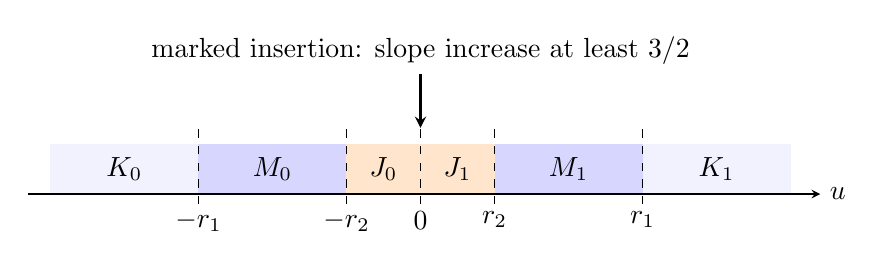
\begin{tikzpicture}[x=.94cm,y=.8cm,>=stealth]
 \fill[blue!5] (-5,0) rectangle (-3,.8);
 \fill[blue!16] (-3,0) rectangle (-1,.8);
 \fill[orange!20] (-1,0) rectangle (1,.8);
 \fill[blue!16] (1,0) rectangle (3,.8);
 \fill[blue!5] (3,0) rectangle (5,.8);
 \draw[->] (-5.3,0)--(5.4,0) node[right] {$u$};
 \foreach \x in {-3,-1,0,1,3} {\draw[dashed] (\x,-.16)--(\x,1.05);}
 \node at (-4,.4) {$K_0$};
 \node at (-2,.4) {$M_0$};
 \node at (-.5,.4) {$J_0$};
 \node at (.5,.4) {$J_1$};
 \node at (2,.4) {$M_1$};
 \node at (4,.4) {$K_1$};
 \node[below] at (-3,-.12) {$-r_1$};
 \node[below] at (-1,-.12) {$-r_2$};
 \node[below] at (0,-.12) {$0$};
 \node[below] at (1,-.12) {$r_2$};
 \node[below] at (3,-.12) {$r_1$};
 \draw[->,thick] (0,1.9)--(0,1.05);
 \node[above,align=center] at (0,1.9) {marked insertion: slope increase at least $3/2$};
\end{tikzpicture}
\caption{The two radial scales, with $r_i=6\log a_i$ and $a_1\ge a_2$.
The central region suppresses both sets of strict roots and is compared
with $J_t$. The next region suppresses only the first set and is compared
with $M_t$; the exterior is compared with $K_t$. The transitions have
width $O(\delta\log k)$ in the proof. The diagram is schematic and does
not depict the exceptional case in which the middle intervals disappear.}
\label{fig:radial-regions}
\end{figure}


\paragraph{Cancellation of the larger scale.}
Each side of the central insertion has length
\((m'-1)D=6\log k-T+O(1)\).
The paired decay is therefore \(k^{-9/8+O(\delta)+O(\varepsilon)}\).
The two intermediate regions have combined length at most
\(12\log(a_1/a_2)+O(T+D)\).  Their rate \(5/288\) contributes
\((a_1/a_2)^{5/24}\).  Since \(a_1\asymp N\) and
\(a_2\asymp k\), all the estimates together give
\[
 \limsup_{u_*\to\infty}\limsup_{P\to\infty}
      \frac{|\mathcal T(P,u_*)|}{\mathcal S}
 \le k^{-9/8}(N/k)^{5/24}\ k^{O_D(\delta)+O_{C_0}(\varepsilon)+o(1)}.
\]
Fixed multiplicative constants are absorbed into the exponent loss.
Equation~\eqref{c4:normalized-two-mark-comparison} now restores the lattice normalization at a cost
\(N^{-5/24+o(1)}\).  Its dependence on the total size cancels:
\[
 k^{-9/8}(N/k)^{5/24}N^{-5/24}=k^{-4/3}.
\]
The condition \(N\le k^{C_0}\) converts all residual \(o(1)\) powers of
\(N\) into \(o(1)\) powers of \(k\).  We first keep \(D\) fixed, then
let \(\delta,\varepsilon\) decrease to zero.  This proves
\eqref{c4:H-bound}, with the stated uniform exponent slack.
\end{proof}

\section{Two prescribed edges and the polygon second moment}\label{c4:metric-consequences}

The analytic estimate is now complete. We identify its normalization
with a positive sum of physical polygons, then sum over displacements
between the two marked edges. Tilted cuts let us treat every displacement
except three lattice directions; those exceptional pairs are controlled
by the first length moment.

\subsection{A tilted cut and its positive two-edge mass}

Use the site order $(P,L,T,R)$ of \eqref{c4:Pair-sum}. Choose a pattern
of $k=a+b$ sites, with $a$ unshifted sites $(z=Q,x=q)$ and $b$ shifted
sites $(z=1,x=1)$, where $1\le b\le a$. Repeat this pattern $m\ge3$
times, with $N=mk$ even, and mark its first and $(k+1)$-st sites.
The marks have the same type, and $L$ is the shorter block between them.

We realize this array at auxiliary parameter $Q^{-1}$ in the ordinary
honeycomb lattice. Tile the plane by rhombi with side vectors $d_j,v$,
where
\[
 h=(\sqrt3,0),\qquad v=(\sqrt3/2,3/2),\qquad
 d_j=\begin{cases}h-v,&z_j=Q,\\h,&z_j=1.\end{cases}
\]
Their lower corners are $\sum_{i<j}d_i+nv$, with $n\in\mathbb Z$ and
the pattern extended in both column directions. Split each rhombus
along its shorter diagonal into two elementary triangles, put a
trivalent vertex at each centroid, and put ports at the outer side
midpoints. At $z_j=1$ the two vertices group bottom-left and right-top
ports; at $z_j=Q$ they group bottom-right and left-top ports. These are
exactly the physical local weights: the resulting dual graph is the
ordinary honeycomb, with weight $x_*$ per visited vertex
\cite{GlazmanManolescu2017,ZhouBatchelor1997}.
The displacement of one pattern is
\[
 d=a(h-v)+bh,
\]
and the cylinder identifies points differing by $md$. The marked edges
cross the cut at the bottom ports of the two marked sites in a fixed row.

\begin{proposition}[Physical meaning of the two-mark scalar]
\label{prop:two-mark-positive}
For this finite-width cylinder,
\begin{equation}
 \mathscr H=
 \sum_{\text{cylinder polygons using both marked edges}}
                              x_*^{|\gamma|}.                         \label{c4:Geom-2}
\end{equation}
The sum includes both contractible and winding polygons, with each
unoriented polygon counted once.
\end{proposition}

\begin{proof}
We first identify the two vacuum factors with physical half-cylinder
states. With twist $\eta=-i$, the no-defect matching transfer is
nonnegative and kills all closed loops. Its powers on the empty state
increase, as for the straight cut. They are bounded as well: each
remaining arc lifts to a planar arch below the zigzag cut and can be
closed by a fixed cap on the other side. Such a cap can be drawn in one
diagram row because bottom-to-bottom turns and horizontal passes have
positive weights for both column types. It joins distinct lifted stubs,
so closing gives a simple polygon through a fixed edge. The total
weight of these polygons is finite by \eqref{c4:Tail}. At fixed width
there are only finitely many endpoint choices for each matching; their
fixed cap lengths therefore bound its coefficient.

Every matching is reachable, by building its arcs from longer to shorter
intervals, using positive top-to-top turns and straight passes. The
rank-one convergence argument in Section~\ref{c4:cylinder} now applies.
Its normalized fixed vector is $\Psi(z)$: the polynomial fixed-vector
identity supplies it, and \eqref{c4:Pair-Pf} ensures regularity at these
sites. For inverse sites and auxiliary $Q^{-2}$ the two column types
are interchanged. The crossed transpose identity on charge zero thus
puts the same physical rows above the cut, with inverse twist and limit
$\Psi(z^{-1})^t$.

It remains to compute the phase of each finite-height diagram.
For an arc with endpoints $j<l$, in either half, its factor is
$q^{s_j}$ with $s_l=-s_j$. For a lower wrapping arc this follows from
\[
 q^{-s_j}\eta^{-s_j}=q^{s_j}.
\]
For upper arcs, use upward-positive spins and inverse twist: traversal
from the left endpoint at positive spin has turn $-2$ in square-diagram
quarter-turn units, with a rightward seam crossing for a wrap. This
gives the same endpoint rule. The pairings are noncrossing in cyclic,
hence chord, order. We may therefore redraw them as semicircles below
and above a horizontal line, with $P$ the leftmost slot. This redraw
computes phases separately for each original diagram. It preserves
connectivity; distinct cylinder diagrams retain their own physical
weights and are not identified, even if their redrawings coincide.

The two half-diagrams have matching spins except at $P,T$, where they
flip. A cycle cannot contain just one flip, so the two marks belong to
one alternating loop. Their prescribed signs orient its two paths
uniquely from $T$ to $P$, with opposite vertical arrival tangents at $P$.
Every other component is a freely oriented Jordan loop disjoint from
the marked component. It cannot separate $P$ from $T$, so its algebraic
intersection with the interval $P<j<T$ is zero. Thus it contributes zero
to $S_L$ in either orientation. Its two turn phases are $-i$ and $i$,
and cancel. Only the marked loop can survive.

For completeness, we compute its phase using the two oriented paths.
If $\gamma$ is either path, rounded to have a continuous unit tangent,
its signed turn satisfies
\[
 W(\gamma)=\Delta\arg(\gamma(t)-T)
                +\Delta\arg(P-\gamma(t)),
\]
with tangent limits at the endpoints. To obtain equality in lifted
arguments, consider the normalized secant
\[
 \frac{\gamma(t)-\gamma(s)}{|\gamma(t)-\gamma(s)|},
                    \qquad 0\le s<t\le1.
\]
Simplicity keeps the off-diagonal secants nonzero, and the regular
rounding gives a continuous extension to the closed ordered-time
triangle, with the unit tangent on the diagonal. A continuous argument
lift on that triangle compares the diagonal with its other two sides, giving
the displayed identity.

Both paths stay strictly to the right of $P$ before arrival. Their
$P-\gamma$ argument changes therefore sum to zero, since the arrival
tangents are opposite. For $\gamma-T$, cut the argument on the negative
horizontal axis. The two initial vertical arguments are opposite, as
are the limiting arguments at $P-T$ from the two half-planes. Every
intermediate cut crossing occurs at a slot $P<j<T$ and contributes
$-2\pi s_j$ to the lifted change. Consequently
\[
 W(\gamma_1)+W(\gamma_2)=-2\pi S_L.
\]
The arc phases have product $\exp(-i(W(\gamma_1)+W(\gamma_2))/4)
=\eta^{-S_L}$, canceling the insertion $\eta^{S_L}$. The marked loop
therefore has coefficient one. Taking the increasing finite-height
limits proves \eqref{c4:Geom-2} and its convergence.
\end{proof}

We now apply Theorem~\ref{c4:thm-two-mark} to these physical arrays.
Let $\iota=1$ if the first pattern site is unshifted and $\iota=0$ if it is
shifted. Omitting the marked sites gives the exact sector counts
\[
 \begin{aligned}
 (a_2,d_2)&=(a-\iota,b-1+\iota),\\
 (a_1,d_1)&=((m-1)a-\iota,(m-1)b-1+\iota).
 \end{aligned}
\]
Since $a\ge k/2$, we have $a_2\asymp k$, $a_1\asymp N$, and
$a_1\ge a_2$, with uniform comparison constants as $k\to\infty$.
Both ratios $d_i/a_i$ differ from $b/a\in[0,1]$ by $O(1/k)$,
uniformly including $b=1$. Hence, for fixed $C_0$ and $N\le k^{C_0}$,
\begin{equation}
                        |\mathscr H|\le k^{-4/3+o(1)}.                \label{c4:Geom-1}
\end{equation}
The exponent slack is uniform over these patterns: a failure for any
fixed positive slack at arbitrarily large $k$ would give a sequence
satisfying every hypothesis of Theorem~\ref{c4:thm-two-mark} and
contradict its conclusion.

\paragraph{Summing the marked displacements.}
Return to the plane translation classes used in \eqref{c4:Tail}.  Write
\(\ell(\gamma)=|\gamma|\) and \(w(\gamma)=x_*^{\ell(\gamma)}\).
\begin{proposition}[Polygon second length moment]\label{c4:prop-polygon-second-moment}
For unoriented simple polygons of the unit-edge honeycomb lattice,
counted modulo translations by \(\mathbb Z h+\mathbb Z v\),
\begin{equation}
                   \sum_{\operatorname{diam}\gamma\le r}|\gamma|^2 w(\gamma)
                             \le r^{2/3+o(1)}.                         \label{c4:Geom-3}
\end{equation}
as \(r\to\infty\), with Euclidean diameter and critical weight
\(w(\gamma)=x_*^{|\gamma|}\).
\end{proposition}

\begin{proof}
We first restrict to a diameter shell
$r/2\le\operatorname{diam}\gamma\le r$. On one fixed sublattice, a
polygon has $\ell(\gamma)/2$ vertices. Partition them by their missing
incident edge, which has three possible types, and let $m$ be the size
of a largest class. Then $m\ge\ell(\gamma)/6$. Let
$\mathcal P(\gamma)$ be the set of all ordered pairs on the chosen
sublattice with the same missing edge type, including diagonal pairs.
It contains the $m^2$ ordered pairs from the largest class, so
\[
             \ell(\gamma)^2\le36m^2\le36\lvert\mathcal P(\gamma)\rvert.
\]
We bound this last pair count by separating short, collinear, and
remaining displacements. Diagonal pairs belong to the short class.

For each first vertex, there are \(O(r)\) lattice vertices at distance
less than \(\sqrt r\).  There are also \(O(r)\) vertices within distance
\(r\) on the three triangular-grid lines through that vertex.  Thus the
pairs with short or collinear displacement contribute at most
\(C r\ell(\gamma)\) per polygon.  Their total shell contribution is
\[
 Cr\sum_{\operatorname{diam}\gamma\ge r/2}\ell(\gamma)w(\gamma)
       =r^{1/3+o(1)},
\]
by \eqref{c4:Tail}.  This is smaller than the required shell bound.

For every remaining pair, translate its first vertex to a fixed vertex
of the chosen sublattice and denote its displacement by \(d\).  A
honeycomb symmetry, followed if necessary by reflection, puts it in the
form
\[
 d=a(h-v)+bh,\qquad a,b\in\mathbb Z_{>0},\qquad b\le a.
\]
The strict positivity follows from having removed the three boundary
directions.  Set \(k=a+b\); then \(k\asymp|d|\), uniformly in the
direction.  The two vertices have the same missing edge type, so they
also share both occupied edge types.  Of these two types, at least one
is perpendicular to one of the two side steps \(h-v,h\).  Sum over the
bounded number of such choices, and start a pattern with that step.
Use \(a\) copies of \(h-v\) and \(b\) copies of \(h\) in the pattern.
Place its first port at the midpoint of the chosen occupied edge at the
first vertex.  Repetition puts the corresponding port at displacement
\(d\), in slot \(k+1\).  Both marked sites have the same type, as required
by the two-mark estimate.

Choose an even integer \(m\ge3\) so that \(N=mk\asymp r\) and
\(|md|>2r\).  Since \(k\gtrsim\sqrt r\), this choice has
\(3k\le N\le k^{C_0}\) for a fixed \(C_0\), after enlarging it to absorb
bounded constants.  Every counted polygon has diameter at most \(r\),
so its projection to this cylinder is injective.  Fixing the first marked
edge recovers its unique plane lift.  In particular, the anchored
polygons at displacement \(d\) count exactly the ordered vertex-pair
choices over translation classes; no factor proportional to the period
is introduced or lost.

Equations~\eqref{c4:Geom-1} and \eqref{c4:Geom-2} consequently bound the
mass for this displacement and edge choice by
\(Ck^{-4/3+o(1)}\), uniformly under the polynomial-width restriction.
For any fixed \(\varepsilon>0\), absorb the uniform exponent loss into
\(k^{\varepsilon}\).  There are \(O(t^2)\) lattice displacements in each
dyadic annulus \(t\le |d|<2t\), and hence
\[
 \sum_{\sqrt r\lesssim |d|\le r}|d|^{-4/3+\varepsilon}
   \le C_\varepsilon
      \sum_{\sqrt r/ C\le 2^j\le 2r}
            (2^j)^{2/3+\varepsilon}
   \le C_\varepsilon r^{2/3+\varepsilon}.
\]
Together with the exceptional-pair estimate this proves the same bound
for the shell.  Sum the shells below \(r\), including the finite
small-diameter contribution.  The resulting geometric series has the
same exponent.  Since \(\varepsilon>0\) was arbitrary, this proves
\eqref{c4:Geom-3}.
\end{proof}

\section{Length cutoffs and open paths}\label{sec:cutoff-laws}

The analytic work is complete. We now use only the positive polygon estimates.

\begin{proof}[Proof of Corollary~\ref{cor:length-cutoffs}]
Use the functions $A$, $P$ and $M_2$ of Theorem~\ref{thm:polygon-tails}, whose bounds have now been proved. All sums below use the same positive polygon weights, and all exponent estimates hold as their argument tends to infinity. We prove

\[
F(n):=\sum_{L\ge n}w=n^{-3/2+o(1)},\qquad
 Q(n):=\sum_{L\ge n}Lw=n^{-1/2+o(1)}.
\]

First consider a length bin $n\le L<2n$ and split it at $D=n^{3/4}$. On its small-diameter part,

\[
\sum w\le n^{-2}M_2(n^{3/4})=n^{-3/2+o(1)}.
\]

On its large-diameter part,

\[
\sum w\le A(n^{3/4})=n^{-3/2+o(1)}.
\]

Multiplying these bounds by $2n$ gives a length-weighted bin bound $n^{-1/2+o(1)}$. Summing the bins $[2^j n,2^{j+1}n)$, $j\ge0$, gives

\[
F(n)\le n^{-3/2+o(1)},\qquad Q(n)\le n^{-1/2+o(1)}.
\]

To justify the infinite sum, first bound every $o(1)$ by an arbitrary fixed positive exponent loss, small enough that both geometric series converge, and then let that loss tend to zero.

For the reverse bounds fix $\delta>0$ and put $R=n^{3(1+\delta)/4}$. The length-weighted mass at diameter at least $R$ is

\[
P(R)=n^{-(1+\delta)/2+o(1)}.
\]

Its contribution from $L<n$ is at most

\[
nA(R)=n^{-1/2-3\delta/2+o(1)},
\]

which is negligible compared with $P(R)$. Its contribution from $L\ge n^{1+2\delta}$ is at most the already proved upper bound

\[
Q(n^{1+2\delta})\le n^{-1/2-\delta+o(1)},
\]

also negligible. Consequently the remaining polygons, with

\[
n\le L<n^{1+2\delta},\qquad D\ge R,
\]

carry length-weighted mass at least $n^{-(1+\delta)/2+o(1)}$. This is a lower bound for $Q(n)$. Dividing it by $n^{1+2\delta}$ gives

\[
F(n)\ge n^{-3/2-5\delta/2+o(1)}.
\]

Letting $\delta$ decrease to zero proves both claimed tail exponents.

Now condition on $L\ge n$. It suffices to prove the claim for $0<\epsilon<3/4$, since any larger tolerance follows from a smaller one. Fix such an $\epsilon$. For the unrooted law, the probability of an excessively large diameter is bounded by

\[
\frac{A(n^{3/4+\epsilon})}{F(n)}
       \le n^{-2\epsilon+o(1)}.
\]

The probability of an excessively small diameter is bounded by

\[
\frac{n^{-2}M_2(n^{3/4-\epsilon})}{F(n)}
       \le n^{-2\epsilon/3+o(1)}.
\]

Both vanish. Under the length-weighted law the corresponding bounds are

\[
\frac{P(n^{3/4+\epsilon})}{Q(n)}
       \le n^{-2\epsilon/3+o(1)},\qquad
 \frac{n^{-1}M_2(n^{3/4-\epsilon})}{Q(n)}
       \le n^{-2\epsilon/3+o(1)}.
\]

The second inequality uses $L\le L^2/n$ on the conditioning event. Thus $D=n^{3/4+o(1)}$ in probability under either law.

Finally condition the length-weighted law on $D\ge R$. Lengths below $R^{4/3-\epsilon}$ have conditional mass at most

\[
\frac{R^{4/3-\epsilon}A(R)}{P(R)}
       \le R^{-\epsilon+o(1)}.
\]

Lengths above $R^{4/3+\epsilon}$ have conditional mass at most

\[
\frac{Q(R^{4/3+\epsilon})}{P(R)}
       \le R^{-\epsilon/2+o(1)}.
\]

This proves $L=R^{4/3+o(1)}$ in probability.

The same conclusions hold with the length cutoff replaced by a power-separated window $[n,n^{1+\delta})$ for any fixed $\delta>0$, because the mass above its upper endpoint is negligible compared with the mass above $n$. Nothing in this proof estimates the mass at one exact length. That additional question requires a local estimate or a separate conditioning argument.
\end{proof}

\subsection{Open paths with fixed nearby endpoints}\label{sec:open-cutoffs}

For plane SAWs between the two vertices of a prescribed nearest-neighbor
bond, adding the bond closes every walk except the one-edge walk into
a polygon. This is
an exact correspondence with polygons containing the fixed edge, up to
the constant length and weight adjustment. For restrictions invariant
under honeycomb symmetries, the fixed-edge polygon mass is one third of
the length-weighted translation-class sum: symmetry equates the three
edge-type totals, and translation within a type enumerates the edges
of each class. Thus these open walks have the typical diameter law under
a large length cutoff and the typical length law under a large diameter
cutoff proved above for length-weighted polygons.

The half-plane walks of Corollary~\ref{cor:boundary-neighbor-mean} use a
different correspondence. Their bounded-change cap injection transfers
\eqref{c4:Geom-3} as an upper bound, in addition to the two diameter tails
already obtained there. Applying the same positive-tail argument gives
length-tail exponent $-3/2+o(1)$ under their critical edge weights,
and typical diameter $n^{3/4+o(1)}$ conditional on length at least $n$.
This is a length-cutoff assertion; it does not assert typical length
conditional only on large diameter under the unrooted weight.

\section{Boundary paths and guide corridors}\label{sec:boundary}
\subsection{Flat boundary estimates: the cylinder loss}\label{c4:boundary-loss}

Our aim is to obtain spatial estimates for critical paths whose endpoints
lie on straight lattice cuts. A port is the midpoint of an edge crossing
such a cut. A path between ports visits vertices in the open domain, and
its weight is
\[
                     w(\gamma)=x_*^{L(\gamma)},\qquad
                x_*=(2+\sqrt2)^{-1/2},
\]
where $L(\gamma)$ counts visited vertices. Thus gluing at a port multiplies
weights exactly. In this section all arch masses use this convention.
Distances along a straight cut are measured in port spacings; Euclidean
and lattice distances differ only by fixed factors.

Let $h_n$ be the total weight of half-plane paths from a fixed boundary
port to the port $n>0$ spacings to its right. We shall prove
\begin{theorem}[Flat boundary arches]\label{a:flat-boundary}\label{thm:boundary-arches}
There are absolute constants $c,C>0$ such that, for every integer $n\ge1$,
\begin{equation}\label{c4:BA}
 \sum_{n\ge1}h_n=h_*:=\frac1{2\cos(3\pi/8)},\qquad
 c n^{-5/4}\le h_n\le C n^{-5/4},\qquad
 h_n[\operatorname{diam}\le Cn]\ge c n^{-5/4}.
\end{equation}
The total mass from a fixed port to any other port of its boundary line,
restricted to paths of diameter greater than $R$, is at most $CR^{-1/4}$
for $R\ge1$.
\end{theorem}
The exponent $5/4$ agrees with the boundary prediction from the
conjectural scaling picture of Lawler, Schramm and Werner, recorded
in~\cite[Section~4]{DuminilCopinSmirnov2012}.
The proof separates two questions. First we compute how much arch mass
is lost when the half-plane is wrapped onto a cylinder of circumference
$N$. This loss is of order $N^{-1/4}$. Then a three-root boundary identity
converts that loss into pointwise estimates and spatial confinement.

\subsubsection{An exact expression for the cylinder arch mass}
We use the $p=1$ vacuum constructed in Section~\ref{c4:vacua}, at
$q=Q^2=e^{i\pi/4}$ and twist $\eta=-i=q^{-2}$. Only even
circumferences are needed here. The polynomial tensor $V_N$ is the raw
vacuum; its empty component is $D=D_1$, and the physical stationary
state is $V_N/D$.

For an arc at ordered endpoints $i<j$, the link-map coefficient is
$q^{s_i}$ for either winding class. Thus the link diagrams may be read
as noncrossing diagrams in a disk. Write the component of the raw
$V_N$ supported just at $i,j$ as $q^{s_i}T_{ij}$, where $s_j=-s_i$.
Define the normalized scalar
\[
 F_N:=D^{-1}\sum_{i<j}z_i z_jT_{ij},\qquad t_i=z_i^2,
 \qquad \mathbf t=(t_i)_i.
\]
We shall prove the rational identity
\begin{equation}
 F_N=h_*\left[\sum_i t_i+\mathbf t^t\mathcal K^{-1}\mathbf1\right],
 \qquad
 \mathcal K_{ij}=\frac{t_i^2-t_j^2}{t_i^2+\sqrt2t_it_j+t_j^2}.
 \label{c4:BC}
\end{equation}
The main step is to prove that $F_N$ is symmetric in the site variables.
A null identity for the vacuum gives this symmetry; the even Pfaffian
formula of Section~\ref{c4:pair-denominator} then determines the scalar
by interpolation.

\paragraph{A covariant raising operator.}
Put $\kappa=Q^6$ and $K|s\rangle=\kappa^s|s\rangle$. Let $e$ raise
spin by one, with coefficients $Q^{-3},1,0$ from $-,0,+$, respectively,
and set
\[
 \mathcal E(z)=\sum_j z_jK_1\cdots K_{j-1}e_j.
\]
Charge conservation and the local identity
\[
 B(r)(r e\otimes I+K\otimes e)
       =(e\otimes I+r K\otimes e)B(r)
\]
make $\mathcal E$ covariant under exchange. To check the local identity,
use the tensors of Section~\ref{c4:local-tensors}. After multiplication
by $r^2g(x)$, $r=e^{ix}$, every entry of its difference is a polynomial
of degree at most five. It vanishes at $r=1,Q^3$; at the second point,
\[
 (e\otimes I+Q^3K\otimes e)C=0,\qquad
 C^t(Q^3e\otimes I+K\otimes e)=0.
\]
The negatives of these points are also roots by spin parity, since
conjugating $e$ by spin parity negates it. The constant term vanishes:
the limiting weighted swap intertwines $K\otimes e$ with $e\otimes I$
because $\xi\kappa=1$, and the extra term supported on
$|+,-\rangle\langle+,-|$ contributes zero on both sides. The reversed
swap at infinity similarly intertwines $e\otimes I$ with $K\otimes e$,
so the degree-five coefficient vanishes. The remaining degree-four
polynomial has the five roots just listed and is zero.

\paragraph{The null identity.}
We claim that $\mathcal E(z)^2V_N=0$. This tensor exchanges covariantly
and rotates with trivial twist. Indeed, for two raises with site
multiplicities $n_i$ summing to two, the order-dependent input phase is
\[
 \kappa^{\sum_i n_i\sum_{j<i}s_j};
\]
for distinct raised sites there is also the constant $1+\kappa$.
Left rotation subtracts $2s_1$ from the exponent on charge-zero inputs,
which is compensated by $\eta^{s_1}=\kappa^{2s_1}$.

At an adjacent positive fusion $z_j=Q^3z_i$, the inserted $C$ is neutral
and is killed by its local two-site raising sum. Induction on the
remaining sites therefore proves the null identity on this slice,
starting with the empty list (the one-site vacuum is killed as well).
Exchange and rotation give vanishing at both pair ratios
$t_j=q^{\pm3}t_i$ for any two sites. After stripping the output-spin
factors, every entry has degree at most $N-1$ in each $t_i$:
an extra power of $t_i$ can arise only from input spin $-$, whose
vacuum degree bound is $N-2$. The $2(N-1)$ pair roots prove the claim
for $N\ge2$.

\paragraph{Symmetry of the arc scalar.}
Take the component of this null identity with output $+,+$ at $1,2$
and vacancies elsewhere. For $2<l<m$, let $Z_{lm}$ be the raw diagram
weight with just the arcs $1m,2l$; equivalently it is the corresponding
$++--$ coefficient divided by $q^2$. Enumerating the raised sites and
dividing by $1+\kappa$ gives
\[
 0=D z_1z_2-h_*(t_1+t_2)T_{12}
   +\sum_{l>2}z_l(Q^{11}z_2T_{1l}+Q^5z_1T_{2l})
   +\sum_{2<l<m}z_lz_mZ_{lm}.
\]
For example, a double raise contributes $Q^{-3}/(1+\kappa)$ times its
diagonal spectral and prefix factors. Two exterior raises require
input $++--$ and multiply its arc phase by $\kappa^3Q^{-6}$.

On exchanging sites $1,2$, the coefficients change by
\[
 \begin{aligned}
 T_{12}&\longmapsto UD+wT_{12},\\
 \binom{T_{1l}}{T_{2l}}&\longmapsto
       (uI+v\,\mathrm{Swap})\binom{T_{1l}}{T_{2l}},\\
 T_{lm}&\longmapsto T_{lm}+UZ_{lm}.
 \end{aligned}
\]
In the last formula, closing $12$ kills a loop, while the nested arcs
join. The change of $DF_N$ is consequently $U$ times the displayed
null component: the needed local scalar equalities, with
$z_1/z_2=e^{ix}$, are
\[
 (v-1)e^{\pm ix}+u=-UQ^{\pm3},\qquad
 (1-w)z_1z_2=Uh_*(t_1+t_2),
\]
which follow by sine addition. Rotation preserves $F_N$, so all
adjacent exchanges preserve it. Thus $DF_N$ is symmetric and
polynomial in the $t_i$ before division by $D$.

\paragraph{Determination by pair fusion.}
The even Pfaffian formula for $D$ in Section~\ref{c4:pair-denominator}
shows that $D\,\mathbf t^t\mathcal K^{-1}\mathbf1$ is symmetric
polynomial of degree at most $N$ in each variable. Here the Pfaffian
cofactors clear kernel poles with the prefactor, and alternation gives
the required Vandermonde divisibility. The polynomial
$D(F_N-h_*\sum_i t_i)$ has the same degree bound.

Place a fused pair adjacent with $t_j=q^3t_i$. The vacuum prescription
makes $F_N$ equal its value on the shorter list plus
$Q^3t_i=h_*(t_i+t_j)$. Meanwhile $\mathcal K_{ij}$ has a pole, with
unrelated entries regular, so its inverse contraction reduces to that
on the shorter list. Symmetry gives the reversed pair ratio too.
Inductively, the difference between the two sides of
\eqref{c4:BC}, after clearing $D$, therefore vanishes at
$2(N-1)>N$ pair nodes for $N\ge4$. The initial case is
$F_2=h_*^{-1}t_1t_2/(t_1+t_2)$, from the two-site vacuum.
This proves \eqref{c4:BC}.

\subsubsection{The size of the homogeneous correction}
The exact formula reduces the cylinder loss to one scalar. Write
\(m_N\) for the homogeneous limit of \(\mathbf t^t\mathcal K^{-1}\mathbf1\). For \(N=2l\),
\begin{equation}
                         -m_N\asymp N^{3/4}.                       \label{c4:BM}
\end{equation}
In log-coordinates the kernel is \(\sinh w/(\cosh w+1/\sqrt2)\), \(w=\log(t_i/t_j)\); its derivative is the cosine transform of the positive even weight
\(\rho(k)=k\cosh(\pi k/4)/\sinh(\pi k)\) on \(\mathbb R\) by the integral used above for \eqref{c4:Pair-Pf}. Take derivative bases in each variable at confluence (equivalently change rows and columns and both contracted vectors by factorial-scaled divided differences before taking the limit). Ordering evens then odds from orders \(0,\ldots,N-1\), the kernel matrix becomes \(\left(\begin{smallmatrix}0&-H\\ H&0\end{smallmatrix}\right)\), \(H_{ab}=(-1)^{a+b}\int k^{2(a+b)}\rho(k)dk,\ 0\le a,b<l\), invertible. The two vectors become all ones and the order-zero unit vector. Hence \(-m_N=\mathcal P_{l-1}(-1,0)\) for the reproducing kernel of polynomials of degree \(\le l-1\) in \(s=k^2\) under \(\rho(k)dk\).

Here are details of this kernel's size. Put \(A_0=3/4\), and compare even probability weights \(\sigma_{1/2},\sigma_1\) proportional to \(1/\cosh(\pi A_0 k)\), \(k/\sinh(\pi A_0 k)\) respectively. The ratio \(\rho/\sigma_1\) is uniformly bounded above and below and decreasing with \(s\), proportional to \(1+\sinh(2u)/\sinh(4u)\), \(u=\pi |k|/4\). The ratio \(\rho/\sigma_{1/2}\) is increasing, proportional to \(u/(\tanh u+\tanh(3u))\). The diagonal kernel \(\mathcal P_{l-1}(0,0)\) is comparable to its \(\sigma_1\) counterpart by the extremal evaluation norm. And \(\mathcal P_{l-1}(s,0)/\mathcal P_{l-1}(0,0)=p(s)/p(0)\) with \(p\) monic orthogonal of degree \(l-1\) for \(s\rho\), by reproducing. At \(s=-1\) this last ratio is bounded below by that for \(s\sigma_1\) and above by that for \(s\sigma_{1/2}\).

We use the classical Markov monotonicity principle for zeros under an increasing weight ratio~\cite{Markoff1886}, and give the derivative argument in the present normalization. The zeros of a monic orthogonal polynomial on \(s>0\) are positive simple by the sign-change test. They all shift increasingly when tilting by an increasing positive ratio \(r(s)\), so the product \(\prod_j(1+1/s_j)=p(-1)/p(0)\) decreases. To see this differentiate along weights \(d\mu_\tau=r(s)^\tau d\mu_0\) (moments and coefficients are smooth here), at a zero \(s_j\) putting \(h_j=p/(s-s_j)\). For any polynomial \(f\) of degree below \(\deg p\), \(\int f h_j\) is \(f(s_j)/h_j(s_j)\) times \(\int h_j^2\) by orthogonality. Differentiating \(\int p h_j=0\) thus gives
\[
 s'_j \int h_j^2\,d\mu_\tau
   =\int (s-s_j)h_j(s)^2(\log r(s)-\log r(s_j))\,d\mu_\tau .
\]
Decreasing ratios similarly reverse the shift.

The comparison polynomials are the Meixner--Pollaczek polynomials $P_d^{(\lambda)}(3k/4;\pi/2)$ in their standard generating-function normalization~\cite[Equation~18.23.7]{DLMF}. We give the orthogonality and norm computation for the probability measures used here.

For \(\sigma_\lambda,\lambda=1/2,1\), orthogonal polynomials \(g_d(k)\) are the coefficients of \(u^d\) in
\[
 (1+u^2)^{-\lambda}\exp(2A_0 k\arctan u),
\]
with squared norms \((2\lambda)_d/d!\) (rising factorial). In fact the moment generating function of \(A_0 k\) at \(y\) is \(\cos(y/2)^{-2\lambda}\): for the hyperbolic secant integrate \(e^{yz}/\cosh(\pi z)\) shifting by \(i\) across \(i/2\); its self-convolution gives density proportional to \(z/\sinh(\pi z)\) by the tanh addition identity. Integrating the product of two generating functions thus gives \((1-uv)^{-2\lambda}\) near zero. These polynomials have the indicated degrees with fixed parity. For \(\lambda=1\), \(g_{2a}(0)=(-1)^a\); thus the diagonal kernel at zero for even degrees through \(2l-2\) is of order \(\log(2+l)\). For \(s\sigma_\lambda\) the desired orthogonal polynomial is proportional to \(g_{2l-1}(k)/k\). At \(k=i\), \(g_d(i)\) has modulus of order \((1+d)^{A_0+\lambda-1}\) at large degrees, from the coefficients of \((1+iu)^{A_0-\lambda}(1-iu)^{-A_0-\lambda}\). Indeed after removing \(i^d\) and dividing by \((A_0+\lambda)_d/d!\), the convolution tends to \(2^{A_0-\lambda}\) since the binomial series of the first factor at 1 converges, and the second sequence is increasing with fixed-shift ratios tending to 1 (summation by parts). At zero,
\[
 |g'_{2l-1}(0)|=2A_0\sum_{a=0}^{l-1}
        \frac{(\lambda)_a}{a!}\frac1{2(l-1-a)+1}
       \asymp l^{\lambda-1}\log(2+l)
\]
by splitting the sum at halfway (the rising-factorial estimates follow by logarithms). Thus both comparisons give normalized ratio of order \(l^{A_0}/\log(2+l)\). This proves \eqref{c4:BM}.

\subsubsection{Recovering the half-plane mass}
At homogeneous sites \(F_N/N\) is the summed arch weight from a specified port on the half-infinite cylinder to ports at strictly positive lifted displacement, by translation, the link fixed-vector identification and counting both lifts (negative endpoints have equal total by reversal/translation). Reflection can put the half-plane above its line. These are exactly the retained arches from that source in the plane half-plane with endpoint to the right, when projecting to a simple arch between distinct ports on the cylinder. Necessarily the span between ends in spacings is \(<N\) by interlacing. The plane total on that side is \(\le h_*\) by the single boundary estimate from the transfer argument. Since \(F_N/N=h_*(1+m_N/N)\), the plane total must be \(h_*\), and the deleted mass for even \(N\) is
\begin{equation}
             d_N\asymp N^{-1/4}.                                   \label{c4:BD}
\end{equation}
Set $X_n=\sum_{j>n}h_j$. An arch whose endpoint displacement
is at least the cylinder period cannot be retained. Consequently
$X_n\le Cn^{-1/4}$, first by comparison with an even period comparable to
$n$, and then for every $n\ge1$. At this stage this is only an upper
bound: a path can be deleted by meeting a translate even when its
endpoint displacement is small. The next argument controls this
additional mechanism.

\subsection{The three-root boundary identity and plane geometry}\label{c4:boundary-geometry}

The cylinder calculation has supplied the tail upper bound. To obtain a
matching lower bound we need to control intersections of two arches with
noninterlacing endpoints. For this purpose we use a boundary identity in
which one of three rooted branches is distinguished. Its local
cancellation is the same honeycomb parafermionic mechanism as the
single-root identity~\cite{DuminilCopinSmirnov2012}.

Domains below are convex lattice-cut domains as in the earlier boundary argument. Put \(\beta=3/8,\ \phi=\pi\beta\). Order boundary ports counterclockwise with outward normal angle lifts \(\theta_j\) (all angle lifts may also be shifted by a common constant). Write \(H(j,d)\) for point-to-point boundary arch weight. For ordered roots \(j_1<j_2<j_3\), if \(j\) is one root and \(a,b\) the other two, put
\[
 P_{jd;ab}=H(j,d)H(a,b)-Z(jd;ab)
\]
with \(Z\) the mutually disjoint two-arch weight (zero if partners coincide with the other arc's ports). Then in finite domains
\begin{equation}
\begin{gathered}
 \sum_{d\ne j}e^{i\beta\theta_d-i\phi\operatorname{sgn}(d-j)}H(j,d)=e^{i\beta\theta_j},\\
 S_j=\sum_{d\ne j}e^{i\beta\theta_d-i\phi\operatorname{sgn}(d-j)}P_{jd;ab},\\
 (S_{j_1},S_{j_2},S_{j_3})=S_{j_1}(1,q,q^2).
\end{gathered}\label{c4:BW}
\end{equation}
The real coefficients after removing the root phase are in \([\cos\phi,1]\).

Here is a direct proof by active-prefix propagation. An unblocked prefix at a vertex distributes its weight with phases \(e^{\pm i\beta\pi/3}\) to its extensions through that vertex at weight \(x_*\) each, by \(2x_*\cos(\beta\pi/3)=1\). Start with phase \(e^{i\beta\theta_j}\). Exit at \(d\) accumulates additional turn \(\theta_d-\theta_j-\pi\operatorname{sgn}(d-j)\), by closing simply along the counterclockwise boundary. Prefixes blocked on themselves (first attempting re-entry into a visited vertex) cancel in pairs: they return by the unused third edge and one reverses the simple loop, keeping the prefix up to that vertex's first arrival. The prefix approaches from outside the loop. Thus the two additional turns through second arrival are \(\pm4\pi/3\) (loop internal turns \(\pm5\pi/3\), first launch turn \(\mp\pi/3\)), giving opposite phases. This gives the single identity. Next propagate with an already present regular arc between \(a,b\). Self-block still cancels. Blocks on that regular arc give three disjoint branches to the blocking vertex, in cyclic order of the roots, with mass independent of which branch was active (central vertex weighted once via the regular arc). Between consecutive roots in increasing order, the turns \(W,W'\) of their branches up to arrival obey \(W-\pi/3-W'=\theta_{j'}-\theta_j-\pi\), by concatenating towards the second root with turn \(-\pi/3\) at the vertex. So the block vector has successive phase ratio \(e^{2\pi i\beta/3}=q\). Subtracting the disjoint exit contributions from the starting weight (single identity times the regular arc mass) identifies this vector summed over blocks as the \(S\)-vector.

These equations pass to the flat half-plane, wedges, and slabs used here by exhausting with convex lattice hexagon cutoffs. Indeed exit on the cutoff has mass tending to zero for a fixed root, even in its whole supporting half-plane, by the positive real single identity and saturation of the flat total proved in \eqref{c4:BD}. Fixed companion arch weights are bounded and all sums absolutely convergent; the limiting remaining phases use the same order of sides as on large cutoffs. On a flat half-plane take the boundary left to right. For three roots there let \(D_j^\pm\) be the sums of deficits in \(S_j\) without phases, over \(d>j\) and \(d<j\) respectively (\(+\) for \(>\)). Then for each pair of consecutive roots in the triple,
\[
              D_{j'}^-=D_j^+,\qquad D_{j'}^+=\sqrt2 D_j^+-D_j^- .
\]
This follows comparing the two real coordinates along \(e^{i\phi},e^{-i\phi}\) in \eqref{c4:BW}. Applied to \(0,n,n+1\) (horizontal units of port spacing), all partners to the right for free root \(n\) interlace or coincide, so \(D_n^+=h_* h_{n+1}=D_{n+1}^-\le h_* h_n\). Thus \(h_n\) is decreasing.

\subsubsection{Collision mass between separated boundary intervals}
Since weights are positive, the deficit $P_{uv;xy}$ is exactly the product
mass of pairs that are not mutually vertex-disjoint. This remains true
when their endpoints interlace: in that case disjoint pairs do not exist.
We shall prove the noninterlaced-interval collision bound
\begin{equation}
 L(n):=\sum_{d>c>n}P_{0 n;cd}\le(\sqrt2-1)X_n^2 .               \label{c4:BL}
\end{equation}
Separate partner locations into $M=(0,n)$ and $R=(n,\infty)$, and put
\[
 \Pi(E,F)=\sum_{A\in E,\ B\in F}P_{0A;nB},\qquad
 \begin{array}{ll}
 p=\Pi(R,R),&v=\Pi(M,R),\\
 g=\Pi(R,M),&w=\Pi(M,M).
 \end{array}
\]
Also write $H_M=h_*-X_n-h_n$ and $t_0=\sqrt2-1$.
We sum the three-root relations over two families of triples.

First take $(0,n,c)$ with $c\in R$. Summing $D_0^+=D_n^-$ gives
\[
 p+v+h_*h_n=g+h_nX_n+X_n^2.
\]
The partners on opposite exterior sides in the right-hand sum
interlace, so their deficits are their full product masses.
The sums of $D_n^+$ and $D_c^+$ are $p$ and $L(n)$, respectively;
the other three-root relation therefore gives
\[
 L(n)=t_0p-v-h_*h_n.
\]

Next take $(0,c,n)$ with $c\in M$. Reflection makes the sums of
$D_c^-$ and $D_c^+$ equal; call their common value $J$. The sums of
$D_0^+$ and $D_0^-$ are $g+w+h_nH_M$ and $v$, respectively, again
using reflection. Hence
\[
 J=g+w+h_nH_M,\qquad v=t_0J.
\]
Substitution into the first family of equalities yields
\[
 p-J=X_n^2-w-t_0J-(2H_M+h_n)h_n.
\]
Every subtracted term is nonnegative. Thus
$L(n)=t_0(p-J)-h_*h_n\le t_0X_n^2$, proving \eqref{c4:BL}.

\subsubsection{A matching arch tail and pointwise decay}
Consider \eqref{c4:BD} at a large even period $m$. Let
$d_m^{\rm small}$ be the deleted mass with endpoint
$1\le n\le\epsilon m$. Each such arch $\gamma$ collides with a
horizontal translate $\gamma+pm$ for some $p\ge1$; fix one
$p=p(\gamma)$ deterministically. Otherwise its cylinder projection
would remain simple. Joining at an intersection gives a simple
crosscut in their union from $n$ to $pm$, above the base and no higher
than the maximum height of $\gamma$.

Take a second independent arch of the same deleted small-endpoint
class, with endpoint $k$, and shift its source to $\delta$. If
$n<\delta<\delta+k<pm$ and its height is at least that of $\gamma$,
it must meet this crosscut: the region cut off against the base has
interior strictly below the crosscut's maximum height. Thus it shares
a vertex with $\gamma$ or $\gamma+pm$. There are at least $cm$
allowed integer shifts when $\epsilon<1/4$ and $m$ is large.
By exchange of the two independent arches, the required height
ordering holds on at least half the product mass.

Charge intersections with $\gamma$ to the corresponding terms of
$L(n)$. For intersections with $\gamma+pm$, shift the second arch
back by $pm$; both of its endpoints then lie left of zero.
Reflection about $n/2$, with reversal of the first arch, puts these
pairs into the reflected version of the same collision sum.
For each fixed first arch, $p(\gamma)$ is fixed and
$\delta\mapsto\delta-pm$ is injective. The charged pair retains
that first arch, so varying $p$ between first arches causes no
additional multiplicity. Summing and using $X_n\le Cn^{-1/4}$ gives
\[
       m(d_m^{\rm small})^2\le C\sum_{n\le\epsilon m} L(n)
          \le C(\epsilon m)^{1/2}.
\]
Thus $d_m^{\rm small}\le C\epsilon^{1/4}m^{-1/4}$. Choose a fixed
$\epsilon>0$ so small that this is less than half the lower bound for
$d_m$ in \eqref{c4:BD}. All remaining deleted paths have endpoint greater
than $\epsilon m$, whence
\[
 X_{\lfloor\epsilon m\rfloor}\ge d_m-d_m^{\rm small}
                         \ge c m^{-1/4}.
\]
Comparison with even $m$ gives $X_n\asymp n^{-1/4}$ for every $n$.
To extract a pointwise estimate, monotonicity first gives
\[
 \lfloor n/2\rfloor h_n
       \le\sum_{j=\lceil n/2\rceil}^{n}h_j
       \le X_{\lceil n/2\rceil-1}\le Cn^{-1/4}
\]
for large $n$. Conversely, choose a fixed $A>1$ so large that
$X_n-X_{\lfloor An\rfloor}\ge c n^{-1/4}$. Then
\[
 c n^{-1/4}\le\sum_{j=n+1}^{\lfloor An\rfloor}h_j
                  \le An\,h_{n+1}.
\]
Absorbing bounded values of $n$ proves $h_n\asymp n^{-5/4}$.
This controls where an arch ends. We next control where it travels.

\subsubsection{Horizontal and vertical excursions}
We first bound horizontal excursion. Let \(U_r\) denote summed arch mass from a given source in its flat half-plane reaching absolute tangential displacement at least \(r\). Endpoints of such order already cost \(O(r^{-1/4})\). Use spacing units, and consider just endpoints \(0<n\le r/4\), excursions to the right reaching \(r\). In each such \(\gamma\) choose a far point of coordinate \(x\ge r\) at a vertex, so reflection across this vertical axis preserves the honeycomb and its boundary ports. Indeed in port-spacing units the vertex coordinates are $i+j/2$ and $i+j/2+1/2$; twice the chosen coordinate is integral, and reflection preserves both sublattices. Take a second independent arch in that class reaching at least the first arch's maximum height, start it at integer \(\delta\) with \(|\delta-x|\le r/8\), and also consider the mirror image of this shifted arch across the chosen vertical axis. Both pairs of endpoints are strictly to the right of \(n\). At least one variant intersects \(\gamma\): up to first reaching the specified height the shifted arch forms a bottom-to-top barrier in the corresponding closed horizontal strip. The chosen point lies on a barrier or to the right of at least one of the two mirrored barriers, while \(\gamma\) starts left of both. Thus by \eqref{c4:BL} again, \(r\) times the square of this class mass costs at most \(C\sum_{n\le r/4} L(n)\) (shifts and their mirrors counted separately for each first arch, reversing orientation as needed). The leftward case is identical with barriers left of both ends, and negative endpoints follow by symmetry. This proves \(U_r\le C r^{-1/4}\).

We next bound the normal-height excursion mass. Let $Y_r$ be the total
weight of arches from a fixed port in its supporting half-plane that
reach normal height at least $r$. Endpoints are free on the boundary
line, and weights still count visited vertices. We work in Euclidean
units; fixed lattice rounding is absorbed into constants.

Take an upward-open wedge $\mathcal W$ of angle $2\pi/3$. In
counterclockwise boundary order its successive side tangents have
angles $-\pi/6$ and $\pi/6$. Choose ports $a$ on the left side and $c$
on the right side, each at distance in $[.25r,.30r]$ from the apex.
For either source, the total wedge mass to the other side is
$O(r^{-1/4})$. Indeed, a normal tube of width a sufficiently small
constant times $r$ from that source stays in the wedge indefinitely.
In the supporting half-plane, an own-side arch lost on restricting to
the wedge must leave this tube. Its mass is at most the already bounded
horizontal excursion mass. Comparing the positive real single-root
identities in the wedge and half-plane therefore bounds the new
opposite-side exits by $Cr^{-1/4}$.

We use this cross-mass bound in the three-root identity. Write
$I_1,I_2,I_3,I_4$ for the successive open boundary intervals obtained
by splitting the left side at $a$ and the right side at $c$. Thus the
boundary order runs down the left side through $I_1,a,I_2$, then up
the right side through $I_3,c,I_4$. Put
\[
 M_{ij}=\sum_{v\in I_i,\ w\in I_j}P_{av;cw},
\]
where the deficits are taken in $\mathcal W$, and write $H(a,c)$ for
the wedge arch mass between the two roots. All entries of $M$ are
nonnegative. With $f(k)=e^{i\pi k/16}$ applied entrywise, put
\[
 A=f(5,-7,-5,-5),\qquad C=f(5,5,7,-5),\qquad R=f(4,8,8,4).
\]
For a third root $z\in I_u$, Equation~\eqref{c4:BW} gives
$S_c=R_uS_a$, with partner phases $C$ and $A$. Summing over $z$ gives
\[
 \sum_j C_jM_{uj}-R_u\sum_i A_iM_{iu}=O(H(a,c)).
\]
The error consists of omitted coincident partners at $a$ or $c$;
their product masses are bounded by the uniformly finite row totals.

The entries with $i=3,4$ and $j=1,2$ have total $O(r^{-1/2})$,
because both arches then cross to the opposite side and their product
is bounded by the two cross-mass totals. For the other entries, take
the dot product of the real parts of the four equations with
$(10,7,-1,-2)$ and of the imaginary parts with $(0,6,0,0)$. The
resulting coefficient matrix is, to within $1/10$ entrywise,
\[
 \begin{pmatrix}
  7.51&8.04&1.12&5.17\\
  .56&.84&8.23&.56\\
  -10.36&-9.71&.64&1.41\\
  -10.92&-10.26&.44&.85
 \end{pmatrix}.
\]
The exact lower bound used here follows directly from the phase
formula. If $a_i,c_j,r_j$ are the displayed integer phase indices and
$\alpha,\nu$ are the real and imaginary multipliers, the coefficient
of $M_{ij}$ is
\[
 \alpha_i\cos\frac{\pi c_j}{16}
 +\nu_i\sin\frac{\pi c_j}{16}
 -\alpha_j\cos\frac{\pi(r_j+a_i)}{16}
 -\nu_j\sin\frac{\pi(r_j+a_i)}{16}.
\]
The half-angle identities show that every coefficient outside the
lower-left $2\times2$ block is at least $2/5$. Positivity of the
entries, together with the bound on that exceptional block, yields
\[
                \sum_{i,j}M_{ij}\le
                   C\bigl(r^{-1/2}+H(a,c)\bigr).
\]
For fixed $a$, the allowed interval for $c$ contains order $r$ ports.
Its total $H(a,c)$ mass is at most $Cr^{-1/4}$ by the cross-mass bound.
We may therefore choose an allowed $c$ with
$H(a,c)\le C r^{-5/4}$.

It remains to put height excursions into this deficit estimate.
Fix a sufficiently small constant $\epsilon>0$. Let $\mathcal E_a$
be the own-half-plane arches from $a$ that reach normal height $r$
and whose points all have tangential displacement less than
$\epsilon r$ from $a$. Define $\mathcal E_c$ in the same way on the
other side, and let $e_a,e_c$ be their raw masses. By symmetry and
the definition of $U_{\epsilon r}$, writing $x_+=\max\{x,0\}$,
\[
             e_a,e_c\ge (Y_r-U_{\epsilon r})_+.
\]
The two narrow normal tubes lie in $\mathcal W$, so these arches are
wedge arches ending on their own sides. The inward normal rays from
$a$ and $c$ cross at normal heights between $.4r$ and $.6r$ on each
ray. Their tubes of tangential half-width $2\epsilon r$ have an overlap
parallelogram. A path in $\mathcal E_a$, being confined to the
narrower tube and reaching height $r$, contains a subpath across one
pair of opposite sides of this parallelogram. A path in
$\mathcal E_c$ crosses the other pair. To see each crossing, follow
the signed tangential coordinate relative to the other normal ray.
At the source and at the first point of normal height $r$, this
coordinate lies on opposite sides of the other wider tube, because
the ray crossing occurs between heights $.4r$ and $.6r$ and the path
stays in its narrower tube. Continuity gives the required subpath.
The two side pairs alternate,
so the two subpaths intersect. In the planar honeycomb embedding
such an intersection includes a shared vertex.

Every pair from $\mathcal E_a\times\mathcal E_c$ is therefore counted
by the deficit for its two endpoints. Those endpoints belong to
unique intervals among the $I_i$, and hence
\[
 (Y_r-U_{\epsilon r})_+^2
       \le e_ae_c
       \le \sum_{i,j}M_{ij}
       \le C\bigl(r^{-1/2}+r^{-5/4}\bigr).
\]
Since $U_{\epsilon r}\le C_\epsilon r^{-1/4}$ for the fixed
$\epsilon$, this proves $Y_r\le C r^{-1/4}$.
Finally, if an arch from a fixed source has diameter greater than
$R$, some point of it is at distance greater than $R/2$ from the
source, up to a bounded port offset. Its tangential displacement or
normal height is then at least a fixed multiple of $R$. The bounds
for $U$ and $Y$ give the raw all-endpoint diameter tail
$O(R^{-1/4})$, with bounded $R$ absorbed into the constant.

\subsubsection{Confinement at a prescribed endpoint}
The radial tail controls the total mass removed by a large truncation.
A finite-domain monotonicity identity will distribute the mass left in
that truncation to each prescribed endpoint. This is the final step in
Theorem~\ref{a:flat-boundary}. In any finite lattice-cut convex truncation with flat side containing \(b<a_1<a_2\) in counterclockwise order there, \(a_1,a_2\) adjacent, cut the ordered list just after \(a_2\), writing \(\theta_A\) for their common angle. In \eqref{c4:BW}, rewrite \(S_{a_i}\) as the single-identity product minus the disjoint terms. Free root \(a_2\) can have a disjoint partner only \(x<b\); free \(a_1\) only \(b<x<a_1\) by noninterlacing, where \(\theta_x=\theta_A\). Thus taking the imaginary part after multiplying \(S_{a_2}=q S_{a_1}\) by \(e^{i\phi-i\beta\theta_A}\) gives
\[
 \sin\phi\,[H(b,a_1)-H(b,a_2)]
     =\sum_{x<b}\sin(\beta(\theta_x-\theta_A+2\pi))Z(ba_1;xa_2)\ge0
\]
since \(q e^{2i\phi}=-1\) and by convexity. Now truncate around a given flat source \(b\) at sufficiently large constant times \(n\), containing that size half-neighborhood up to bounded rounding. The just-proved radial tail and \(h_j\asymp j^{-5/4}\) leave mass \(\gtrsim n^{-1/4}\) to same-side endpoints \(b+j,\ j\in[n,2n]\). Monotonicity along the side in this truncation yields \eqref{c4:BA}, increasing the diameter constant for bounded \(n\) as needed.

\subsection{Slab and corridor estimates}\label{c4:corridors}

We now pass from arches with both endpoints on one cut to bridges between
two parallel cuts. We first bound their total and pointwise mass, then
retain a comparable total mass inside a prescribed narrow corridor.

Fix a lower port and an integer height $h\ge1$. In the slab and corridor
coordinates below, measure both coordinates in units of the distance
between consecutive parallel cuts; thus $h$ counts those gaps.
A bridge visits only vertices of the open slab and ends at a port of its
upper cut. Write $\mathcal B_h$ for this set of bridges. Let $B_h(x)$ be
its total critical mass at signed horizontal
displacement $x$, and let $B_h=\sum_xB_h(x)$. The horizontal variable lies
in the fixed displacement lattice of the chosen cuts. We set
$B_0(x)=\mathbf1_{\{x=0\}}$ when using convolution.

The vanishing of the critical strip bridge mass was proved
in~\cite{BeatonEtAl2014}; a polynomial upper bound was later obtained
in~\cite{KrachunPanagiotis2026}. The bounds below identify its decay
up to constant factors and retain a comparable mass inside the
prescribed corridors.

\begin{theorem}[Spatial bridge estimates]\label{a:bridge-spatial}\label{thm:slab-corridors}
For all $h\ge1$ and every allowed horizontal displacement $x$,
\begin{equation}\label{a:bridge-estimates}
 c h^{-1/4}\le B_h\le C h^{-1/4},\qquad
 B_h(x)\le C h^{-5/4},\qquad
 B_h[\operatorname{diam}>Mh]\le C(Mh)^{-1/4}\quad(M\ge1).
\end{equation}
Let $g:[0,1]\to\mathbb R$ be a continuous piecewise linear function with
$g(0)=0$, and fix $\varepsilon>0$. The bridge mass restricted to the
corridor
\[
 \left\{(x,y):0\le y\le h,\quad
                  |x-hg(y/h)|\le\varepsilon h\right\}
\]
is at least $c(g,\varepsilon)h^{-1/4}$ for all sufficiently large
admissible $h$. The starting port is fixed and the terminal port is free.
For a compact family of such graphs in the uniform topology, the constant
and the lower threshold can be chosen uniformly.
\end{theorem}
The same conclusions hold after a lattice symmetry. The weights still
count visited vertices, so no endpoint factor appears when bridges are
joined at ports.

All cuts can be taken on straight lines of the triangular grid dual to the honeycomb (so portals are at edge midpoints, including for convex wedges and lattice-hexagon truncations). Write \(t=3/8,\ \phi=\pi t\). We use the preceding flat boundary estimates \(h_n\asymp n^{-5/4}\), \(\sum_{n>0}h_n=1/(2\cos\phi)\), radial arch tail \(O(R^{-1/4})\), and the confined lower bound \(h_n[\operatorname{diam}\le C n]\ge c n^{-5/4}\), from any port in its half-plane. Recall that in convex domains the single boundary identity has all positive real coefficients \(\in[\cos\phi,1]\) after removing the root phase, determined by the boundary normals; in particular same flat side gets \(\cos\phi\). It and the three-port deficit identity pass to wedges (angle \(\pi/3\) or \(2\pi/3\)) and slabs by exhaustion: the weight of free arms escaping via a truncating hexagon at distance of order \(R\) is \(O(R^{-1/4})\) per root. Indeed compare with the same truncation of its own half-plane, where this follows by the single identity and flat radial tail; fixed accompanying arcs have uniformly bounded weight.

\subsubsection{Total mass and diameter tightness}
Slab total bridge weight \(B_h\) from a bottom port across \(h\) levels is \(\le C h^{-1/4}\), by the single identity comparing to the full half-plane (the loss of same-side arches). Its portion of diameter \(>M h\) is \(O((M h)^{-1/4})\) by subtracting the identity in a slab truncated by the hexagon (both bottom and top losses are positive). For lower bounds, in a wedge from a port at distance comparable to \(k\) from the apex on one side, mass of walks to the other side is \(\asymp k^{-1/4}\), still with lower bound for diameter \(\le C k\). Indeed all own-side endpoints beyond the apex are lost from the half-plane, whereas a fixed-radius fraction of a \(k\)-neighborhood at the port stays in the wedge on its half-plane side; compare the single identities as before. Truncation loses at most \(C'(C k)^{-1/4}\). Summing such cross weights over ports at distances in \([k,2k]\) on one side gives \(\gtrsim k^{3/4}\); by reversal and the upper bound, ports on the other side within distance \(\delta k\) of the apex cost at most \(C(\delta k)^{3/4}\). Take \(\delta>0\) small. Cutting the wedge by a parallel to the first side \(h\) levels inward, for \(k\) a sufficiently large fixed multiple of \(h\), deletes those targets further than \(\delta k\). Thus by the single identities the new top exits, of weight at most \(B_h\) per source, compensate the lost weight with coefficients bounded positively. This gives \(B_h\gtrsim h^{-1/4}\).

\subsubsection{A bound uniform in the upper endpoint}
For the pointwise upper bound fix opposite roots \(a,c\) (bottom, top). In boundary order the four open classes labeled successively \(1,2,3,4\) are the bottom split at \(a\) (order left to right) and the top split at \(c\) (right to left), normal angles \(-\pi/2,\pi/2\). Write \(P_{av;cw}\) for the deficit, product of the two arch weights minus their joint disjoint weight, and \(M_{ij}=\sum_{v\in i,w\in j}P_{av;cw}\). Put \(F(k)=e^{i\pi k/16}\) entrywise, \(A=F(3,-9,-3,-3)\), \(C=F(3,3,9,-3)\), \(r=F(4,8,8,4)\). The three-root identity at \(a,c,z\) has integrated complex deficits \(S_j\) for each choice of free root, i.e. the sum over its partner with factors \(\exp(it\theta_{\rm partner}\pm i\phi)\) (plus before the root); for increasing roots these \(S\)'s are in ratio \(1:q:q^2,\ q=e^{i\pi/4}\). Thus for \(z\in u\), \(S_c=r_u S_a\). Summing,
\[
 \sum_j C_j M_{uj}-r_u\sum_i A_i M_{iu}=O(H(a,c)),
\]
where \(H(a,c)\) is the point-to-point bridge weight; the errors are omitted coincident partners \(a\) or \(c\) weighted by products, bounded using the uniformly finite row totals. These equations bound all entries by \(O(B_h^2+H(a,c))\). Indeed exceptions \(i=3,4,\ j=1,2\) already cost \(B_h^2\); take the dot product with \((2,2,-2,-7)\) on the real parts and \((0,2,-3,0)\) on imaginary parts. The coefficient of $M_{ij}$ is given by the same explicit trigonometric
formula used in the wedge, with the present phase indices and
multipliers. Every coefficient outside the lower-left $2\times2$ block
exceeds $1/2$. Half-angle substitution proves this finite list of
inequalities; thus the nonnegative entries have total
$O(B_h^2+H(a,c))$. For a third root $z$ on the bottom, positivity after removal of its
root phase makes $|S_z|$ comparable to the sum of its deficits. Place
$a$ at horizontal coordinate zero and choose $z$ in a bottom interval of
length comparable to $\delta h$ to the left of $a$, and its partner $w$
in such an interval to the right. Here $\delta>0$ is a sufficiently small
fixed constant. The endpoints of $zw$ and $ac$ interlace, so their
deficit is the full product. The confined arch bound gives mass
$c h^{-5/4}$ for each pair $(z,w)$ inside the slab: its diameter is at
most $C\delta h<h$. There are order $h^2$ such pairs. Consequently
\[
 \sum_z |S_z|\ge c_1 h^{3/4}H(a,c).
\]
For each triple the three-root identity gives $|S_z|=|S_c|$.
The previous entry bound, with the omitted endpoint terms restored,
therefore gives
\[
 c_1h^{3/4}H(a,c)\le C_1\bigl(B_h^2+H(a,c)\bigr).
\]
For large $h$ absorb the last term into the left side and use
$B_h^2\le Ch^{-1/2}$. This proves $H(a,c)\le Ch^{-5/4}$ uniformly in
$c$; the uniformly bounded row sums cover the finitely many smaller
heights.

\subsubsection{Corridors in a fixed normal direction}
We first confine bridges around the upward normal. It is important here
to remove the multiplicity caused by choosing intermediate cuts; merely
multiplying layer masses would count the same bridge many times.

Choose a large fixed integer $m$, and let each of the $m-1$ intermediate
seams vary in a short lattice interval around its height $jh/m$. These
intervals are disjoint, have lengths comparable to $h/m$, and ensure
that every successive gap is comparable to $h/m$. The diameter estimate
and the lower bound for $B_t$ show that, for a sufficiently large fixed
$C_2$, bridges across a gap $t$ with diameter at most $C_2t$ have mass at
least $c t^{-1/4}$. Reflection lets us retain at least half this mass with
endpoint displacement directed toward the vertical axis. At every seam
the endpoint is then within $C_3h/m$ of that axis, and each intervening
piece stays within $C_4h/m$. Choosing $m$ sufficiently large places the
concatenation in the desired corridor. The interiors of its pieces lie
in disjoint open layers, so the concatenation is self-avoiding.

Let $K(\gamma)$ be the number of allowed choices of the $m-1$ marked
seams in an output bridge. Summing over the seams and then over the
layer bridges yields
\[
 \sum_\gamma w(\gamma)K(\gamma)
       \ge c_m h^{m-1-m/4}.
\]
To bound the multiplicity we use only the total bridge upper bound.
Write $N(\gamma)$ for the number of internal cuts crossed exactly once.
For every fixed integer $s\ge0$ (with $N^0=1$),
\begin{equation}\label{a:renewal-cut-moment}
 \sum_{\gamma\in\mathcal B_h}w(\gamma)N(\gamma)^s
                         \le C_s h^{-1/4+3s/4}.
\end{equation}
Indeed, after ordering $j\le s$ distinct marked cuts, splitting the path
at them produces $j+1$ bridges of positive heights summing
to $h$. Summing their intermediate endpoints is bounded by the product
of their total bridge masses. One height is at least $h/(j+1)$, hence contributes at most
$C_jh^{-1/4}$. Summing each of the other heights up to $h$ contributes
at most $\sum_{t\le h}B_t\le Ch^{3/4}$. The bounded number of orderings
and coincidences gives \eqref{a:renewal-cut-moment}. Every marked seam
of the construction is crossed once, so $K\le N^{m-1}$.
Cauchy--Schwarz now gives the mass of its unmarked outputs as at least
\[
 \frac{\bigl(c_mh^{m-1-m/4}\bigr)^2}
      {C_mh^{-1/4+3(2m-2)/4}}=c'_m h^{-1/4}.
\]
This proves the corridor lower bound for the normal direction.

The same argument concatenates any fixed finite list of directions for
which corridor lower bounds have already been obtained. For a convex
combination of two slopes, use sufficiently fine but fixed alternating
layers in the corresponding proportions. The polygonal staircase stays
within the desired tolerance of the intermediate slope; choose each
constituent tolerance smaller than the remaining tolerance. Applying
this separately to the finitely many linear pieces gives piecewise
linear guides, with small relative perturbations of the seams allowed.
It remains to obtain sufficiently many slopes.

\subsubsection{Changing the cut normal}
Let \(n,n'\) be upward unit cut normals at angle \(\pi/3\), and suppose narrow corridors have weight \(\gtrsim h^{-1/4}\) in slabs normal to \(n'\) for a forward direction with projected height on \(n\) equal to \(\alpha>0\) per unit height on \(n'\). We transfer that forward direction to a slab on \(n\) of physical height \(H\). Take two internal parallel \(n'\)-cuts. Choose a starting port \(x_1\) of the first at \(n\)-height in \([\delta H,2\delta H]\); separate the second cut by a physical \(n'\)-height \(D\) with \(\alpha D/H\in[1-5\delta,1-4\delta]\). Between them use the directed corridor bridge from \(x_1\) with very small tolerance compared to \(\delta\); its endpoint \(x_2\) is now within \([c\delta H,C\delta H]\) in height distance from the top and the corridor stays inside the outer slab. Join \(x_1\) to the bottom in the wedge before the first cut and above the bottom, and \(x_2\) to the top after the second cut and below the top. Junction masses are \(\gtrsim H^{-1/4}\) each with diameters \(\le C_3\delta H\), by the wedge estimates. Pieces cannot intersect by the tilted cuts. Taking \(\delta\) sufficiently small depending on the desired outer tolerance and slopes confines all this to the required guide corridor relative to the bottom endpoint.

\begin{figure}[htbp]
\centering
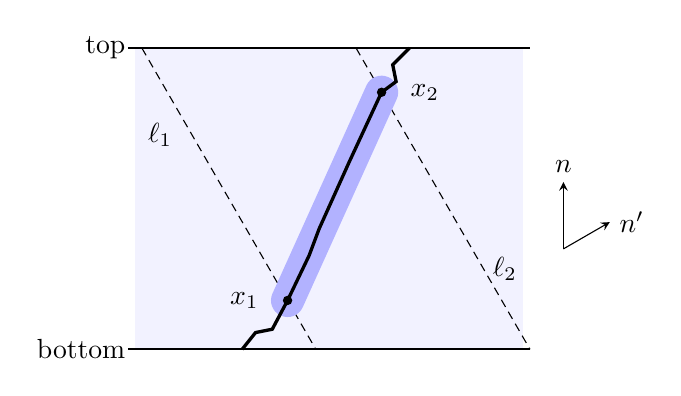
\begin{tikzpicture}[scale=.85,>=stealth]
 \fill[blue!5] (-1.5,0) rectangle (4.3,4.5);
 \draw[thick] (-1.6,0)--(4.4,0);
 \draw[thick] (-1.6,4.5)--(4.4,4.5);
 \node[left] at (-1.5,0) {bottom};
 \node[left] at (-1.5,4.5) {top};
 \coordinate (xone) at ({1.2-.73/sqrt(3)},.73);
 \coordinate (xtwo) at ({4.4-3.84/sqrt(3)},3.84);
 \draw[densely dashed] ({1.2-4.5/sqrt(3)},4.5)--(1.2,0);
 \draw[densely dashed] ({4.4-4.5/sqrt(3)},4.5)--(4.4,0);
 \draw[blue!30,line width=12pt,line cap=round]
        (xone)--(xtwo);
 \draw[very thick] (.1,0)--(.3,.25)--(.55,.3)--(xone);
 \draw[very thick] (xone)--(1.1,1.4)--(1.25,1.8)--(1.7,2.8)--(xtwo);
 \draw[very thick] (xtwo)--(2.4,4)--(2.35,4.25)--(2.6,4.5);
 \fill (xone) circle (2pt) node[left,xshift=-7pt] {$x_1$};
 \fill (xtwo) circle (2pt) node[right,xshift=7pt] {$x_2$};
 \draw[->] (4.9,1.5)--(4.9,2.5) node[above] {$n$};
 \draw[->] (4.9,1.5)--({4.9+.8*sqrt(3)/2},1.9) node[right] {$n'$};
 \node[left] at (-.8,3.2) {$\ell_1$};
 \node[right] at (3.7,1.2) {$\ell_2$};
\end{tikzpicture}
\caption{Changing the cut normal. The middle bridge follows a narrow
corridor between the tilted cuts $\ell_1,\ell_2$; the exterior pieces lie in separate
wedges. Each marked cut is crossed once. The diagram is schematic: the
thick lines indicate the three path pieces, not individual lattice edges.}
\label{a:tilted-corridor}
\end{figure}

Count the three-piece constructions modulo translations along the
bottom cut. In this quotient, the first crossing port $x_1$ has only
finitely many lattice residues at each permitted height, and there
are order $H$ such heights. Independently, the permitted interval
for $D$ contains order $H$ spacings. For each such port and gap, the
product of the three piece masses is at least a constant times
$H^{-3/4}$. Translate each resulting bottom endpoint to the prescribed root, retaining the two tilted cuts as
marks. The output with those marks recovers the crossing ports and
all three pieces, so this translation is bijective on the quotient.
If $K(\gamma)$ denotes the number of resulting marked representations
of the rooted output $\gamma$, then
\[
 \sum_\gamma w(\gamma)K(\gamma)\ge cH^{5/4}.
\]

For the second moment, take two representations of one output and
order their $k\le4$ distinct tilted cuts. The first is one of the
two first cuts and the last is one of the two second cuts; their
crossing ports therefore remain at distances comparable to $\delta H$
from the bottom and top, respectively. The rooted path starts before
every marked cut and finishes after every marked cut. Since each is
crossed exactly once, the crossings occur in the cut order, and the
intervening pieces stay in their open tilted slabs.

Again count modulo bottom translations. There are $O(H)$ choices
of the first crossing-port orbit. Reverse the first exterior piece:
its bottom endpoint is then free, and the wedge row bound sums that
endpoint with mass at most $CH^{-1/4}$. The last wedge has the same
uniform bound on its retained top-distance band. The original
junction diameters are $O(\delta H)$ and each original middle gap
is $O(H)$, so every spacing between consecutive cuts in the combined
list is at most $CH$. For each fixed spacing, intermediate crossing
ports are already summed by the total bridge mass $B_t$. Summing
positive spacings therefore costs at most
\[
 \sum_{1\le t\le CH}B_t\le C'H^{3/4}
\]
per internal layer. Keep the last-port distance restriction until
applying its uniform wedge bound, and drop the remaining restrictions
for an upper bound. Thus the contribution from $k$ distinct cuts is
at most
\[
 CH\,(H^{-1/4})^2(H^{3/4})^{k-1}
                      =CH^{-1/4+3k/4}.
\]
There are only finitely many ways to assign these cuts to the two
ordered mark pairs, including coincident cuts. Consequently
\[
 \sum_\gamma w(\gamma)K(\gamma)^2\le CH^{11/4}.
\]
Cauchy--Schwarz removes the marks and leaves total mass at least
\[
 \frac{(cH^{5/4})^2}{CH^{11/4}}=c'H^{-1/4}.
\]
All seam choices use their lattice spacings, which agree in physical
units by symmetry. Bounded rounding inside fixed positive relative
intervals changes only the constants.

From the straight corridor and this step we have guides at \(\pm60^\circ\) to any normal, hence also between them by mixtures. Transferring again from the appropriate tilted normal now covers any slope strictly forward on the original one. Concatenation as above gives the piecewise linear form. For uniformity, fix the tolerance $\varepsilon$ and cover the compact
family by finitely many uniform balls of radius $\varepsilon/3$ centered
at its graphs. Carry out the construction for each center with tolerance
$\varepsilon/3$, and take the minimum of the finitely many lower-bound
constants and the maximum of their lower height thresholds. Each
resulting corridor lies in the $\varepsilon$-corridor of any graph in its ball. This proves Theorem~\ref{a:bridge-spatial}.

\begin{thebibliography}{99}
\addcontentsline{toc}{section}{\refname}
\small
\setlength{\itemsep}{2pt}
\bibitem{BeatonEtAl2014}
N.~R. Beaton, M.~Bousquet-M\'elou, J.~de Gier, H.~Duminil-Copin and A.~J. Guttmann.
The critical fugacity for surface adsorption of self-avoiding walks on
the honeycomb lattice is $1+\sqrt2$.
\emph{Communications in Mathematical Physics} \textbf{326} (2014), 727--754.
\href{https://doi.org/10.1007/s00220-014-1896-1}{doi:10.1007/s00220-014-1896-1}.

\bibitem{DuminilCopinSmirnov2012}
H.~Duminil-Copin and S.~Smirnov.
The connective constant of the honeycomb lattice equals $\sqrt{2+\sqrt2}$.
\emph{Annals of Mathematics} \textbf{175} (2012), 1653--1665.
\href{https://doi.org/10.4007/annals.2012.175.3.14}{doi:10.4007/annals.2012.175.3.14}.

\bibitem{Frenkel1985}
I.~B. Frenkel,
\emph{Representations of Kac--Moody algebras and dual resonance models},
in \emph{Applications of Group Theory in Physics and Mathematical Physics}
(Chicago, 1982), Lectures in Applied Mathematics \textbf{21},
American Mathematical Society, Providence, RI, 1985, 325--353.
\href{https://cpb-us-w2.wpmucdn.com/campuspress.yale.edu/dist/2/3739/files/2021/06/frenkel_representations_kac_moody.pdf}{Author's copy}.

\bibitem{FrenkelKac1980}
I.~B. Frenkel and V.~G. Kac,
\emph{Basic representations of affine Lie algebras and dual resonance models},
Invent. Math. \textbf{62} (1980), 23--66.
\href{https://doi.org/10.1007/BF01391662}{doi:10.1007/BF01391662}.

\bibitem{GarbaliNienhuis2017Ground}
A.~Garbali and B.~Nienhuis.
The dilute Temperley--Lieb $O(n=1)$ loop model on a semi infinite strip:
the ground state.
\emph{Journal of Statistical Mechanics: Theory and Experiment} (2017), 043108.
\href{https://doi.org/10.1088/1742-5468/aa6a30}{doi:10.1088/1742-5468/aa6a30}.
\href{https://arxiv.org/abs/1411.7020}{arXiv:1411.7020}.

\bibitem{GarbaliNienhuis2017Sum}
A.~Garbali and B.~Nienhuis.
The dilute Temperley--Lieb $O(n=1)$ loop model on a semi infinite strip:
the sum rule.
\emph{Journal of Statistical Mechanics: Theory and Experiment} (2017), 053102.
\href{https://doi.org/10.1088/1742-5468/aa6bc3}{doi:10.1088/1742-5468/aa6bc3}.
\href{https://arxiv.org/abs/1411.7160}{arXiv:1411.7160}.

\bibitem{GlazmanManolescu2017}
A.~Glazman and I.~Manolescu.
Self-avoiding walk on $\mathbb Z^2$ with Yang--Baxter weights:
universality of critical fugacity and 2-point function.
\emph{Annales de l'Institut Henri Poincar\'e, Probabilit\'es et Statistiques}
\textbf{56} (2020), 2281--2300.
\href{https://doi.org/10.1214/19-AIHP1024}{doi:10.1214/19-AIHP1024}.

\bibitem{GrimmPearce1993}
U.~Grimm and P.~A.~Pearce.
Multi-colour braid--monoid algebras.
\emph{Journal of Physics A: Mathematical and General} \textbf{26} (1993), 7435--7460.
\href{https://doi.org/10.1088/0305-4470/26/24/018}{doi:10.1088/0305-4470/26/24/018}.
\href{https://arxiv.org/abs/hep-th/9303161}{arXiv:hep-th/9303161}.

\bibitem{HammersleyWelsh1962}
J.~M.~Hammersley and D.~J.~A.~Welsh.
Further results on the rate of convergence to the connective constant of
the hypercubical lattice.
\emph{Quarterly Journal of Mathematics} \textbf{13} (1962), 108--110.
\href{https://doi.org/10.1093/qmath/13.1.108}{doi:10.1093/qmath/13.1.108}.

\bibitem{Klich2002}
I. Klich,
\emph{Full counting statistics: An elementary derivation of Levitov's formula},
2002.
\href{https://arxiv.org/abs/cond-mat/0209642v1}{arXiv:cond-mat/0209642v1}.

\bibitem{KrachunPanagiotis2026}
D.~Krachun and C.~Panagiotis.
Quantitative sub-ballisticity of self-avoiding walk on the hexagonal lattice.
\emph{Annals of Probability} \textbf{54} (2026), 1109--1125.
\href{https://doi.org/10.1214/24-AOP1730}{doi:10.1214/24-AOP1730}.

\bibitem{LawlerSchrammWerner2004}
G.~F. Lawler, O.~Schramm and W.~Werner.
On the scaling limit of planar self-avoiding walk.
In \emph{Fractal geometry and applications: a jubilee of Beno\^it Mandelbrot},
Part~2, Proceedings of Symposia in Pure Mathematics \textbf{72}, Part~2,
American Mathematical Society, Providence, RI, 2004, 339--364.
\href{https://arxiv.org/abs/math/0204277}{arXiv:math/0204277}.

\bibitem{Markoff1886}
A. Markoff,
\emph{Sur les racines de certaines \'equations. Seconde note},
Mathematische Annalen \textbf{27} (1886), 177--182.
\href{https://doi.org/10.1007/BF01452056}{doi:10.1007/BF01452056}.

\bibitem{Nienhuis1982}
B.~Nienhuis.
Exact critical point and critical exponents of $O(n)$ models in two dimensions.
\emph{Physical Review Letters} \textbf{49} (1982), 1062--1065.
\href{https://doi.org/10.1103/PhysRevLett.49.1062}{doi:10.1103/PhysRevLett.49.1062}.

\bibitem{DLMF}
NIST Digital Library of Mathematical Functions,
Version 1.2.8, 15 September 2026,
Sections~18.19 and~18.23.
\url{https://dlmf.nist.gov/18.23}.

\bibitem{Segal1981}
G. Segal,
\emph{Unitary representations of some infinite dimensional groups},
Comm. Math. Phys. \textbf{80} (1981), 301--342.
\href{https://doi.org/10.1007/BF01208274}{doi:10.1007/BF01208274}.

\bibitem{ZhouBatchelor1997}
Y.~K.~Zhou and M.~T.~Batchelor.
Critical behaviour of the dilute $O(n)$, Izergin--Korepin and dilute
$A_L$ face models: Bulk properties.
\emph{Nuclear Physics B} \textbf{485} (1997), 646--664.
\href{https://doi.org/10.1016/S0550-3213(96)00654-2}{doi:10.1016/S0550-3213(96)00654-2}.
\href{https://arxiv.org/abs/cond-mat/9611156}{arXiv:cond-mat/9611156}.

\end{thebibliography}
\end{document}
